%% ==========================================================================
%%  SUPERPOSITION, CONTRACTION, AND THE GEOMETRY OF MOTION
%%  A Textbook on Tangent-Space Methods for Nonlinear Dynamics and Control
%% ==========================================================================
\documentclass[10pt,letterpaper,openany]{book}

%% ---------- Page geometry ----------
\usepackage[margin=1in,headheight=14pt]{geometry}

%% ---------- Fonts and encoding ----------
\usepackage[T1]{fontenc}
\usepackage[utf8]{inputenc}
\usepackage{lmodern}
\usepackage{microtype}

%% ---------- Mathematics ----------
\usepackage{amsmath,amssymb,amsthm,mathtools,bm}

%% ---------- Graphics and figures ----------
\usepackage{graphicx}
\usepackage{tikz}
\usetikzlibrary{arrows.meta,calc,decorations.markings,positioning}

%% ---------- Tables ----------
\usepackage{booktabs}
\usepackage{listings}
\usepackage{tcolorbox}
\tcbuselibrary{theorems, breakable, skins}
\usepackage{../geometry_of_motion}
\usepackage{array}
\gomdeclarealgorithms

%% ---------- Lists ----------
\usepackage{enumitem}

\gomapplylistingstyle

%% ---------- Headers and footers ----------
\usepackage{fancyhdr}
\pagestyle{fancy}
\fancyhf{}
\fancyhead[LE]{\small\itshape\leftmark}
\fancyhead[RO]{\small\itshape\rightmark}
\fancyfoot[C]{\thepage}
\renewcommand{\headrulewidth}{0.4pt}

%% ---------- Colors ----------
\usepackage{xcolor}
\definecolor{chapblue}{RGB}{0, 70, 130}
\definecolor{accentred}{RGB}{180, 40, 40}
\definecolor{softgray}{RGB}{245, 245, 245}
\definecolor{trajgreen}{RGB}{30, 130, 60}
\definecolor{darkgold}{RGB}{160, 120, 20}
\definecolor{purplehaze}{RGB}{100, 40, 140}

%% ---------- Hyperlinks ----------
\usepackage[hidelinks,bookmarksnumbered]{hyperref}
\usepackage{imakeidx}
\makeindex[intoc, title=Index]
\hypersetup{
  pdftitle={Tangent-Space Methods for Nonlinear Control and Biomechanics},
  pdfsubject={Tangent-space methods for nonlinear dynamics and control},
  pdfkeywords={contraction theory, tangent hyperplanes, superposition,
               affine systems, LQR, DDP, Riccati, biomechanics, robotics}
}

%% ---------- Colored boxes for remarks, intuition, etc. ----------

\newtcolorbox{intuitionbox}[1][]{%
  colback=blue!5!white,
  colframe=blue!60!black,
  fonttitle=\bfseries,
  title={Geometric Intuition},
  #1
}



\newtcolorbox{warningbox}[1][]{%
  colback=red!5!white,
  colframe=red!60!black,
  fonttitle=\bfseries,
  title={Common Misconception},
  #1
}

\newtcolorbox{designbox}[1][]{%
  colback=orange!5!white,
  colframe=orange!60!black,
  fonttitle=\bfseries,
  title={Design Implication},
  #1
}

\newtcolorbox{axiombox}[1][]{%
  colback=violet!5!white,
  colframe=violet!60!black,
  fonttitle=\bfseries,
  title={#1},
}








\newtcbtheorem[number within=chapter]{laymansbox}{In Plain Language}{
  colback=green!5!white, colframe=green!50!black,
  fonttitle=\bfseries, separator sign={.~},
  breakable
}{laymans}

\makeatletter
\theoremstyle{plain}
\@ifundefined{theorem}{\newtheorem{theorem}{Theorem}[chapter]}{}
\@ifundefined{proposition}{\newtheorem{proposition}[theorem]{Proposition}}{}
\@ifundefined{lemma}{\newtheorem{lemma}[theorem]{Lemma}}{}
\@ifundefined{corollary}{\newtheorem{corollary}[theorem]{Corollary}}{}

\theoremstyle{definition}
\@ifundefined{definition}{\newtheorem{definition}[theorem]{Definition}}{}
\@ifundefined{example}{\newtheorem{example}[theorem]{Example}}{}
\@ifundefined{assumption}{\newtheorem{assumption}[theorem]{Assumption}}{}

\theoremstyle{remark}
\@ifundefined{remark}{\newtheorem{remark}[theorem]{Remark}}{}
\makeatother

%% ---------- Notation Concordance — Volume I ----------
%% This volume uses tangent-space notation conventions:
%%   Vectors:    bold italic via \vec{} (redefined to \bm{})  e.g. \x = \vec{x}
%%   Reals:      \R  (alias for \Reals — both available via geometry_of_motion.sty)
%%   Lie groups: \SO, \SE are parameterless — caller writes \SO(3), \SE(3) explicitly
%%   Transpose:  \T (sans-serif T)
%%   Matrices:   \mat{A} = \mathbf{A}
%%
%% Key differences from other volumes:
%%   - Uses \x, \q, \uvec shorthand (not \state, \control)
%%   - Uses \mat{} wrapper instead of bare \mathbf{}
%%   - \SO, \SE do NOT include (3) — write \SO(3) at the call site
%%
%% See geometry_of_motion.sty for the canonical fallback definitions.
%% ─────────────────────────────────────────────────────

%% ---------- Custom commands ----------
\renewcommand{\R}{\mathbb{R}}
\newcommand{\N}{\mathbb{N}}
\renewcommand{\dd}{\mathrm{d}}

\DeclareMathOperator*{\argmin}{arg\,min}
\DeclareMathOperator*{\argmax}{arg\,max}

\renewcommand{\norm}[1]{\left\lVert #1 \right\rVert}
\newcommand{\abs}[1]{\left\lvert #1 \right\rvert}
\renewcommand{\inner}[2]{\left\langle #1,\, #2 \right\rangle}
\renewcommand{\T}{\mathsf{T}}   % transpose
\newcommand{\trace}{\operatorname{tr}}
\newcommand{\diag}{\operatorname{diag}}
\newcommand{\rank}{\operatorname{rank}}
\renewcommand{\SO}{\mathrm{SO}}
\renewcommand{\SE}{\mathrm{SE}}
\newcommand{\ad}{\mathrm{ad}}
\newcommand{\E}{\mathbb{E}}

%% Bold vectors and matrices
\renewcommand{\vec}[1]{\bm{#1}}
\renewcommand{\mat}[1]{\mathbf{#1}}
\newcommand{\x}{\vec{x}}
\newcommand{\q}{\vec{q}}
\newcommand{\uvec}{\vec{u}}
\newcommand{\y}{\vec{y}}
\newcommand{\dx}{\delta\vec{x}}
\newcommand{\du}{\delta\vec{u}}
\newcommand{\dq}{\delta\vec{q}}
\newcommand{\xx}{\mathbf{x}\mathbf{x}}
\newcommand{\uu}{\mathbf{u}\mathbf{u}}
\newcommand{\xu}{\mathbf{x}\mathbf{u}}

%% Operators
\DeclareMathOperator{\Span}{span}
\DeclareMathOperator{\sym}{sym}
\DeclareMathOperator{\skewpart}{skew}
\renewcommand{\dt}{\dd t}

%% ---------- Chapter style ----------
\usepackage{titlesec}
\titleformat{\chapter}[display]
  {\normalfont\huge\bfseries}
  {\chaptertitlename\ \thechapter}{20pt}{\Huge}
\titlespacing*{\chapter}{0pt}{-20pt}{30pt}

% Reserve space for multi-digit chapter/section numbers in the contents.
\makeatletter
\renewcommand*{\l@section}{\@dottedtocline{1}{1.5em}{3.6em}}
\renewcommand*{\l@subsection}{\@dottedtocline{2}{5.1em}{4.2em}}
\makeatother

%% ==========================================================================
\hypersetup{colorlinks=true, linkcolor=chapblue, filecolor=magenta, urlcolor=chapblue, citecolor=accentred}

\begin{document}
\hypersetup{pageanchor=false}

%% ---------- Title page ----------
\begin{titlepage}
\centering
\vspace*{2cm}

{\Huge\bfseries Tangent-Space Methods for\\[6pt]
Nonlinear Control and Biomechanics\par}

\vspace{1.5cm}

{\Large\itshape Tangent-Space Methods for Nonlinear\\[4pt]
Dynamics and Control\par}

\vspace{3cm}


\vspace{2cm}

{\large\itshape
A unified treatment of how first-order dynamics,\\[4pt]
contraction metrics, and optimal control\\[4pt]
share a common geometric foundation.\par}

\vfill

{\large Draft Edition --- \today\par}
\end{titlepage}

%% ---------- Front matter ----------
\frontmatter
\hypersetup{pageanchor=true}

%% Epigraph / Dedication
\thispagestyle{empty}
\vspace*{\fill}
\begin{center}
\begin{minipage}{0.7\textwidth}
\centering
\itshape
A derivative isolates first-order response. A finite prediction must also account
for nonlinear remainders, numerical error, and the limits of the physical model.
\end{minipage}
\end{center}
\vspace*{\fill}
\newpage

%% Preface
\chapter{Preface}

This book studies how nearby motions respond to changes in preparation, input and physical parameters. First variations belong to tangent spaces and obey linear equations about a specified nominal trajectory. This allows their responses to be combined while retaining the coupling between coordinates. Predicting finite changes in the full nonlinear motion requires an additional accuracy assessment.

The mathematical derivative is an exact first-order object when it exists. Computing it numerically, integrating a differential equation and optimizing a local surrogate introduce separate approximations. Taylor remainders depend on the represented field, direction and scaling; they are not generally intrinsic manifold curvature. These distinctions are necessary when an elegant geometric argument is used to explain a measured golf swing or a humanoid maneuver.

The chapters connect variational dynamics, metrics, contraction analysis, local optimal control and the interpretation of drift and input contributions. Each supplies a different part of the investigation. An affine partition does not identify muscle activity, a local optimizer does not certify a global optimum, and a smooth calculation must be extended when contact events alter the motion.

The treatment is aimed at graduate students and practicing engineers who have encountered linearization, Lyapunov stability, and optimal control as separate topics and want to see them unified. We assume familiarity with linear algebra, multivariable calculus, and ordinary differential equations. Differential geometry is introduced as needed, always paired with physical intuition.

Physical questions motivate the calculations. Worked models, counterexamples and numerical checks distinguish mathematical identities from finite predictions and empirical claims. The reader should know which quantity a calculation explains, which assumptions it needs, and what independent evidence would test its application.

A complete model needs explicit states, units, reference frames, actuator conventions, feasible contacts and a measurable task. The foundations chapter establishes these requirements and the distinction between flow sensitivity and geometric transport. Later chapters develop the additional structure needed for stability, optimization and biomechanical interpretation.

\vspace{1cm}
\hfill\textit{September 2026}

%% Table of contents
\tableofcontents
\chapter*{Nomenclature}
\addcontentsline{toc}{chapter}{Nomenclature}
\markboth{Nomenclature}{Nomenclature}

\section*{General Conventions}
\begin{itemize}
    \item Scalars are lowercase or Greek letters (e.g., $m, t, \theta$).
    \item Vectors are bold lowercase (e.g., $\mathbf{x}, \mathbf{u}, \mathbf{q}$).
    \item Matrices are bold uppercase (e.g., $\mathbf{A}, \mathbf{B}, \mathbf{M}, \mathbf{J}$).
    \item Expected values and sets are denoted by blackboard bold or script (e.g., $\mathbb{E}, \mathcal{S}$).
\end{itemize}

These are default conventions; each chapter declares its model, frames, and
any local reuse of symbols. The mechanical entries below use $n$ independent,
regular local configuration coordinates and $\mathbf{v}=\dot{\mathbf{q}}$.
This convention is local: it does not identify every configuration manifold
with a Euclidean space or apply unchanged to redundant representations.

\section*{State and Kinematics}
\begin{description}
    \item[$\mathbf{q} \in \mathbb{R}^n$] Configuration coordinates in the declared local chart.
    \item[$\dot{\mathbf{q}} \in \mathbb{R}^n$] Coordinate rates; the generalized velocities under the local convention above.
    \item[$\ddot{\mathbf{q}} \in \mathbb{R}^n$] Second time derivatives of these coordinates, not necessarily Cartesian point accelerations.
    \item[$\mathbf{x} \in \mathbb{R}^{n_x}$] State-vector representation with $n_x$ components; commonly $\mathbf{x} = [\mathbf{q}^T, \dot{\mathbf{q}}^T]^T$ locally, with actuator or internal states added when needed. Redundant state representations also retain their constraints.
    \item[$\mathbf{u} \in \mathbb{R}^m$] Control input vector (e.g., joint torques, muscle activations).
    \item[$\boldsymbol{\tau} \in \mathbb{R}^n$] Generalized forces conjugate to $\mathbf{q}$, with power $\boldsymbol{\tau}^T\dot{\mathbf{q}}$; components need not all be joint torques.
    \item[$t \in \mathbb{R}$] Time.
\end{description}

More generally, write $\mathbf{q}\in\mathbb{R}^{n_q}$ for a configuration
representation and $\mathbf{v}\in\mathbb{R}^{n_v}$ for generalized velocities,
with $\dot{\mathbf{q}}=\mathbf{N}(\mathbf{q})\mathbf{v}$ on the admissible domain.
A unit quaternion has four components with a norm constraint, while angular
velocity has three components in a declared frame. Configuration rates and
generalized velocities therefore need not have the same dimension. See
\href{https://underactuated.mit.edu/multibody.html}{Tedrake's multibody notes}
for this representation convention. Constraints and any time-dependent
kinematics must be included in the chosen model.

\section*{Inertia and Dynamics}
\begin{description}
    \item[$\mathbf{M}(\mathbf{q})$] Mass (inertia) matrix. It is symmetric positive definite for independent regular velocities with strictly positive modeled kinetic energy for every nonzero velocity. Constrained, redundant, massless, or singular representations require their own treatment.
    \item[$\mathbf{C}(\mathbf{q}, \dot{\mathbf{q}})$] Coriolis/centrifugal matrix; $\mathbf{C}\dot{\mathbf{q}}$ is the generalized velocity-product force in the local mechanical equation. The matrix factorization is not unique.
    \item[$\mathbf{g}(\mathbf{q})$] Generalized gravity term; its sign follows the side of the mechanical equation on which the chapter places it.
    \item[$\mathbf{J}(\mathbf{q})$] Coordinate Jacobian of a time-independent task map $\mathbf{p}(\mathbf{q})$, so $\dot{\mathbf{p}}=\mathbf{J}\dot{\mathbf{q}}$ in the stated coordinates and frames.
\end{description}

With $\dot{\mathbf{q}}=\mathbf{N}\mathbf{v}$, the corresponding velocity Jacobian is
$\mathbf{J}_v=\mathbf{J}_q\mathbf{N}$. Force components must change with the velocity convention:
$\boldsymbol{\tau}_v=\mathbf{N}^T\boldsymbol{\tau}_q$ gives
$\boldsymbol{\tau}_v^T\mathbf{v}=\boldsymbol{\tau}_q^T\dot{\mathbf{q}}$.
Thus the same club-point motion and mechanical power must result from
consistently paired kinematic and force representations.

\section*{Control and Optimization}
For the indexed entries, declare a discrete update
$\mathbf{x}_{k+1}=F_k(\mathbf{x}_k,\mathbf{u}_k)$ and a nominal pair
$(\bar{\mathbf{x}}_k,\bar{\mathbf{u}}_k)$. Its derivatives are evaluated at
that pair. These are derivatives of the full update, including the chosen
sampling or numerical integration rule, not of zero-input drift alone.
\begin{description}
    \item[$\mathbf{A}_k = D_x F_k$] State Jacobian of the declared discrete update at the nominal pair.
    \item[$\mathbf{B}_k = D_u F_k$] Input Jacobian of that update at the same pair.
    \item[$V(\mathbf{x})$ or $\mathcal{V}$] Value function or Lyapunov function.
    \item[$\mathbf{Q}$] State penalty matrix in LQR/DDP.
    \item[$\mathbf{R}$] Control penalty matrix in LQR/DDP.
    \item[$\mathbf{K}$] Feedback gain matrix ($\delta\mathbf{u} = -\mathbf{K}\delta\mathbf{x}$).
    \item[$\boldsymbol{\gamma}$] A curve with a declared parameter; a timed state trajectory $\boldsymbol{\gamma}(t)$ fixes an initial state and input law. A solution map $\phi(t;t_0,\mathbf{x}_0)$ instead retains dependence on initial time and state, for a fixed evolution law on its domain of existence.
\end{description}

Continuous-time chapters define their Jacobians from the full differential
equation. Some use $f(\mathbf{x},\mathbf{u},t)$ for that full right-hand side;
the autonomous $f(\mathbf{x})$ below denotes only the declared zero-input drift.
Neither convention makes a discrete input Jacobian equal to the continuous
one without accounting for the sampling interval and evolution.

\section*{Affine Control and Counterfactuals}
\begin{description}
    \item[$f(\mathbf{x})$] Drift vector field: complete autonomous evolution of the declared effective plant when $\mathbf{u} = \mathbf{0}$.
    \item[$G(\mathbf{x})$] Input (control) matrix field mapping control inputs to state derivatives.
    \item[$\dot{\mathbf{x}} = f(\mathbf{x}) + G(\mathbf{x})\mathbf{u}$] Control-affine system equations of motion.
    \item[$\mathbf{x}^{\mathrm{ZTCF}}(t)$] Forward Zero-Torque Counterfactual trajectory under $\mathbf{u}(t) \equiv \mathbf{0}$.
    \item[$\mathbf{a}_{\mathrm{ZVCF}}(\mathbf{q}, \mathbf{z})$] Instantaneous Zero-Velocity Counterfactual acceleration with velocity and declared control set to zero.
    \item[$\mathrm{DCR}_{W,\mathcal{U}}(\mathbf{x})$] Drift-Control Ratio in a declared acceleration or task-projected space:
    \[
      \mathrm{DCR}_{W,\mathcal{U}}(\mathbf{x})
      =\frac{\|W \mathbf{a}_{\mathrm{drift}}\|_2}{\sup_{\mathbf{u}\in\mathcal{U}}\|W B_a \mathbf{u}\|_2 + \varepsilon}.
    \]
\end{description}

\section*{Biomechanics and Motor Control}
\begin{description}
    \item[{$a_i \in [0, 1]$}] Muscle activation level.
    \item[$\ell_i^M$] Muscle fiber length.
    \item[$v_i^M$] Muscle fiber contraction velocity.
    \item[$\ell_i^{MT}$] Musculotendon unit length.
    \item[$\mathbf{F}_{\text{muscle}}$] Force generated by muscles.
    \item[$\mathbf{W}$] Muscle synergy matrix (weights).
    \item[$\mathbf{c}(t)$] Muscle synergy activation vector over time.
\end{description}

\section*{Geometry and Manifolds}
\begin{description}
    \item[$SE(3)$] Special Euclidean group of rigid body motions.
    \item[$SO(3)$] Special Orthogonal group of 3D rotations.
    \item[$\mathfrak{se}(3)$] Lie algebra of $SE(3)$, space of spatial twists (velocities).
    \item[$\mathcal{M}$] A smooth manifold.
    \item[$T_{\mathbf{x}}\mathcal{M}$] Tangent space at point $\mathbf{x}$.
\end{description}


%% ---------- Main matter ----------
\mainmatter

%% Include chapters
\chapter[Foundations: Tangent Spaces and Exactness]{Foundations:\\Tangent Spaces and Exactness}
\label{ch:foundations}

\begin{laymansbox}{Zooming in on the Map}{tangent_patch}
A tangent vector describes the direction and rate of a change at one state. A derivative
describes how that change affects another quantity. These are exact mathematical objects
when the required derivatives exist. Using them to predict a finite change is a further
step, whose accuracy must be checked. For a golfer or humanoid robot, that distinction
lets us ask precise questions about sensitivity without pretending that a whole swing
is linear or that a computed derivative validates the underlying physical model.
\end{laymansbox}

\section{Motivation: Why Geometry Matters for Control}

A configuration specifies an arrangement; a state must additionally contain the information
needed to predict its evolution under specified inputs. Joint angles alone do not determine
the next instant of a swing. Joint rates, muscle activation, shaft deformation and modal
rates can all matter. Contact mode and constitutive assumptions determine which states
and forces are admissible. Geometry supplies the language for representing these objects
and comparing nearby motions consistently.

For a homogeneous linear equation $\dot x=A(t)x$, combinations of solutions are solutions.
For $\dot x=A(t)x+B(t)u$, the corresponding initial conditions and inputs must also be
combined. Adding two responses to the same nonzero input generally doubles that forcing.
For a nonlinear system, trajectories expressed in Euclidean coordinates can still be
added algebraically, but the result generally does not solve the same dynamics; on a
general manifold, adding states has no intrinsic definition.

First variations obey a different rule. If $x(t,\epsilon)$ is a differentiable family of
solutions, then $\delta x(t)=\partial_\epsilon x(t,\epsilon)|_{\epsilon=0}$ belongs to the
tangent space at the nominal state. The equation for this derivative is linear in
$\delta x$ and the input variation. Its solutions superpose about the \emph{same} nominal
trajectory. Off-diagonal coefficients still couple wrist, shoulder, shaft and other
coordinates: linear superposition does not mean those coordinates evolve independently.

\begin{figure}[htbp]
\centering
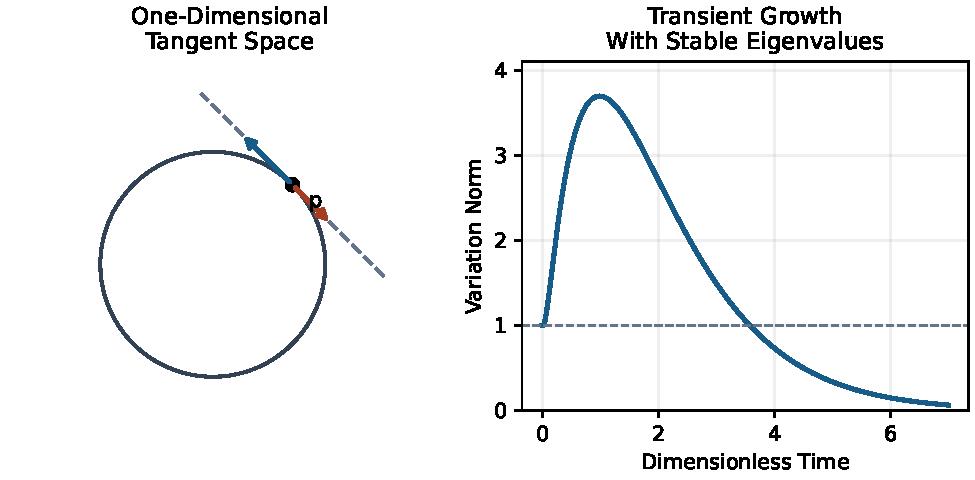
\includegraphics[width=\linewidth]{../figures/foundations_tangent_gain.pdf}
\caption{Tangent Vectors and Finite-Time Amplification. Left: A One-Dimensional Circle Has a Tangent Line. Right: A Stable Linear System Can Amplify a Variation Before It Decays.}
\label{fig:foundations:tangent-gain}
\end{figure}

A tangent space of an $n$-dimensional smooth manifold is $n$-dimensional. A curve has a
tangent line, not a two-dimensional tangent plane. For an embedded surface, a translated
tangent plane can touch the surface at a regular point, but is not a finite patch contained
in it. Corners, intersecting branches and other nonsmooth sets require additional care.
For an abstract manifold, no surrounding Euclidean space or literal touching plane is
required. The figure is an embedded illustration, not the definition.

\section{From the Scalar Derivative to a State-Space Model}

For a scalar function, differentiability at $x_0$ means the limit
\begin{equation}
f'(x_0)=\lim_{h\to0}\frac{f(x_0+h)-f(x_0)}{h}
\label{eq:ch1:derivative-limit}
\end{equation}
exists. Its tangent line is the affine graph
\begin{equation}
y-f(x_0)=f'(x_0)(x-x_0).
\label{eq:ch1:tangent-line}
\end{equation}
The derivative is a linear map on displacements; the tangent-line function includes an
offset. In several variables the analogous statement is
\begin{equation}
f(\bar x+\delta x)=f(\bar x)+Df(\bar x)\delta x+o(\|\delta x\|).
\label{eq:ch1:frechet-heuristic}
\end{equation}
This defines differentiability at a point. It does not by itself assert continuity of the
derivative nearby. A $C^1$ map has continuous first derivatives; $C^2$ has continuous
second derivatives; smooth, without further qualification, normally means $C^\infty$.
We state the finite regularity actually needed below.

The numerical components in these equations depend on coordinates. Differentiability is
preserved by compatible differentiable charts with differentiable inverses. An arbitrary
smooth parameterization need not be a valid coordinate change: $z=x^3$ has zero derivative
at zero and its inverse is not differentiable there. The chain rule makes the derivative
an intrinsic map between tangent spaces; it does not make every displayed matrix or scalar
slope independent of the chart.

There is no conflict between calling a derivative an exact first-order object and calling
its use for a finite displacement an approximation. These are standard complementary
statements. Analytical differentiation, automatic differentiation of implemented code,
finite differences and numerical integration have different computational errors. None
of them establishes that an assumed muscle, contact or shaft model matches a person.

\section{Smooth Dynamical Systems}

In a local chart consider
\begin{equation}
\dot x=F(x,u,t),\qquad x\in\mathbb R^n,\quad u\in\mathbb R^m.
\label{eq:ch1:dynamics}
\end{equation}
On a manifold, $F(x,u,t)\in T_x\mathcal M$. Time-independent examples below omit $t$.
The mechanical state space may be a tangent bundle, with additional activation or internal
variables. It must not be confused with the smaller configuration manifold.

\begin{assumption}[Regularity on a Fixed Mode]\label{ass:smoothness}
On an open neighborhood of the nominal trajectory and admissible perturbations, assume
$F$ is continuous in time and $C^1$ in state and input, with continuous derivatives.
Use a finite interval on which nearby solutions exist in this neighborhood. Assume $C^2$
in the perturbed arguments for the quadratic Taylor bounds below.
\end{assumption}

These are sufficient working conditions, not the weakest possible ones. Local Lipschitz
regularity in state gives local uniqueness under the usual time regularity assumptions;
continuous first derivatives provide it locally. Piecewise continuous prescribed inputs
can also be handled interval by interval. If a feedback law is used, differentiate the
closed-loop field, including the derivative of the law where it exists.

Regular holonomic constraints can define a smooth reduced manifold. Fixed sticking contacts
can admit smooth constrained equations while the contact remains feasible and its Jacobian
has constant rank. Thus a hard constraint does not automatically destroy differentiability.
Touchdown, slip, liftoff, saturation boundaries and impacts require checking mode-specific
regularity and the transition law. These events are central to golf and humanoid mechanics,
so the smooth calculation must have an explicit boundary of application.

\section{The Fréchet Derivative: Definition and Computation}

\subsection{Definition and Uniqueness}

At fixed $(\bar x,\bar u,t)$, the state Jacobian\index{Jacobian} is
\begin{equation}
A=D_xF(\bar x,\bar u,t)\in\mathbb R^{n\times n},
\label{eq:ch1:jacobian-A}
\end{equation}
provided a linear map $A$ satisfies
\begin{equation}
F(\bar x+\delta x,\bar u,t)=F(\bar x,\bar u,t)+A\delta x+r(\delta x),
\label{eq:ch1:frechet}
\end{equation}
with
\begin{equation}
\lim_{\delta x\to0,\,\delta x\ne0}\frac{\|r(\delta x)\|}{\|\delta x\|}=0.
\label{eq:ch1:frechet-limit}
\end{equation}
The limit is over all approaches, not a selected finite set of directions. Norms must be
declared; fixed norms are equivalent for existence of the derivative in finite dimensions,
but numerical magnitudes and condition numbers depend on scaling.

\begin{proposition}[Uniqueness of the Fréchet Derivative]\label{prop:frechet-unique}
There is at most one such linear map $A$.
\end{proposition}
\begin{proof}
If $A$ and $A'$ both satisfy the condition, subtract their expansions to obtain
\begin{equation}
(A-A')\delta x=r'(\delta x)-r(\delta x)=o(\|\delta x\|).
\label{eq:ch1:diff-matrices}
\end{equation}
For fixed $v\ne0$ set $\delta x=sv$ with $s>0$. Then
\[
\|(A-A')v\|\leq
\left(\frac{\|r'(sv)\|+\|r(sv)\|}{s\|v\|}\right)\|v\|\longrightarrow0.
\]
The left side is independent of $s$, hence is zero. This holds for every $v$, so $A=A'$.
\end{proof}

\subsection{Directional Derivatives and Uniformity}

The directional limit
\begin{equation}
D_vF(\bar x)=\lim_{s\to0}\frac{F(\bar x+sv)-F(\bar x)}{s}
\label{eq:ch1:gateaux}
\end{equation}
equals $Av$ when the Fréchet derivative exists. The term Gâteaux derivative is often
reserved for a directional-derivative map that is linear in $v$; even that condition need
not give the uniform remainder required here. For example, define the scalar function
\[
h(x,y)=\begin{cases}x^4y/(x^6+y^2),&(x,y)\ne(0,0),\\0,&(x,y)=(0,0).
\end{cases}
\]
The inequality $2|x^3y|\leq x^6+y^2$ gives $|h(x,y)|\leq|x|/2$, proving continuity
at the origin. Along any fixed ray $(x,y)=s(a,b)$, $h(sa,sb)/s\to0$; this is immediate
when $b=0$ and follows from an $s^2$ factor when $b\ne0$. All directional derivatives
therefore form the zero linear map. But along $y=x^3$, $h=x/2$, and for $x>0$
\[
\frac{|h(x,x^3)|}{\sqrt{x^2+x^6}}=\frac{1}{2\sqrt{1+x^4}}\longrightarrow\frac12.
\]
The function is not Fréchet differentiable there. Testing several directions numerically
cannot replace the assumptions or proof of a uniform limit.

\subsection{The Input Jacobian and Joint Perturbations}

The input Jacobian\index{Jacobian} is
\begin{equation}
B=D_uF(\bar x,\bar u,t)\in\mathbb R^{n\times m},
\label{eq:ch1:jacobian-B}
\end{equation}
and satisfies
\begin{equation}
F(\bar x,\bar u+\delta u,t)=F(\bar x,\bar u,t)+B\delta u+o(\|\delta u\|).
\label{eq:ch1:frechet-u}
\end{equation}
Joint differentiability yields the combined derivative $[A\ B]$ and a joint remainder in
$(\delta x,\delta u)$. Separate derivatives at one point alone do not guarantee this.
For a control-affine field $F=f(x,t)+G(x,t)u$, $B=G(\bar x,t)$, whereas
\[
A=D_xf(\bar x,t)+\sum_i\bar u_iD_xg_i(\bar x,t).
\]
Dropping the second term would omit state-dependent input transmission. Exact affinity in
joint torque also does not imply affinity in muscle excitation: activation dynamics and
force-length-velocity laws intervene between those inputs.

\section{Worked Example: A Dimensioned Pendulum}

Use a point mass $m$ on a massless rigid rod of length $\ell$, angle $\theta$ from downward
vertical, gravity $g$, applied torque $u$ and viscous torque $-c\omega$. Moment balance about
the fixed pivot gives
\begin{equation}
\dot\theta=\omega,\qquad m\ell^2\dot\omega=-mg\ell\sin\theta-c\omega+u.
\label{eq:ch1:pendulum-dyn}
\end{equation}
Here $u$ is in N\,m, $c$ in N\,m\,s/rad and $I=m\ell^2$ in kg\,m$^2$. For a distributed
pendulum replace $I$ by its pivot inertia and $m\ell$ in gravity torque by mass times
pivot-to-center-of-mass distance. The point-mass state field is
\begin{equation}
F(x,u)=\begin{pmatrix}\omega\\-(g/\ell)\sin\theta-(c/I)\omega+u/I\end{pmatrix}.
\label{eq:ch1:pendulum-f}
\end{equation}
At a static equilibrium, $\bar\omega=0$ and $\bar u=mg\ell\sin\bar\theta$. At any state,
not only an equilibrium, the derivatives are
\begin{equation}
A=\begin{pmatrix}0&1\\-(g/\ell)\cos\bar\theta&-c/I\end{pmatrix},
\label{eq:ch1:pendulum-A}
\end{equation}
\begin{equation}
B=\begin{pmatrix}0\\1/I\end{pmatrix}.
\label{eq:ch1:pendulum-B}
\end{equation}
These coefficients expose distinct effects: geometry changes the gravity derivative;
damping changes the rate derivative; inertia scales torque authority. A high existing
angular rate does not reduce $B$ in this model.

For an illustrative numerical case, set $m=1$kg, $\ell=1$m, $g=10$m/s$^2$,
$c=0.1$N\,m\,s/rad and $\bar\theta=\pi/6$. Then $I=1$kg\,m$^2$, $\bar u=5$N\,m and
$A_{21}=-5\sqrt3$ s$^{-2}$, evaluated without rounding in the residual calculation.
For an angle perturbation $d$ with unchanged rate and torque, the only nonzero residual is
\[
r_\omega(d)=-10[\sin(\pi/6+d)-\sin(\pi/6)-\cos(\pi/6)d]
=2.5d^2+\frac{5\sqrt3}{6}d^3+O(d^4).
\]
At $d=0.01$rad, the true acceleration change is approximately $-0.086351099093$rad/s$^2$,
the first-order change is $-0.086602540378$rad/s$^2$, and the residual is
$0.000251441285$rad/s$^2$. The ratio $r_\omega/d^2$ approaches $2.5$ s$^{-2}$ (radians treated as dimensionless), while
$r_\omega/d\to0$. Mixing a rounded matrix with high-precision field evaluations can
create a spurious first-order error at small $d$.

\begin{table}[htbp]
\centering
\caption{Pendulum Residuals With an Unrounded Analytic Jacobian}
\label{tab:foundations:pendulum}
\begin{tabular}{@{}rrrr@{}}
\toprule
$d$ (rad) & $r_\omega$ (rad/s$^2$) & $r_\omega/d$ (s$^{-2}$) & $r_\omega/d^2$ (s$^{-2}$/rad) \\
\midrule
$0.1$ & $0.02642183$ & $0.2642183$ & $2.642183$ \\
$0.01$ & $0.0002514413$ & $0.02514413$ & $2.514413$ \\
$0.001$ & $2.501443\times10^{-6}$ & $0.002501443$ & $2.501443$ \\
$0.0001$ & $2.500144\times10^{-8}$ & $0.0002500144$ & $2.500144$ \\
\bottomrule
\end{tabular}
\end{table}

Angles, angular rates and forces are different physical quantities. A Euclidean norm of
their raw numerical coordinates silently chooses units and relative weights. A declared
scale matrix $S$ defines dimensionless variations $S^{-1}\delta x$; a positive-definite
metric $W$ defines $\|\delta x\|_W^2=\delta x^TW\delta x$. The scalar ratios above use
only angle and angular-acceleration components, with their units retained.

\section{Tangent Spaces as Vector Spaces}
\index{Tangent Space}\index{Manifold}

\subsection{Curves, Charts, and Derivations}
\label{def:tangent-space}
Let $p$ lie in a smooth $n$-manifold $\mathcal M$ and let $\psi$ be a chart near $p$.
Two curves through $p$ represent the same tangent vector if
\begin{equation}
\left.\frac{d}{ds}\psi(\gamma_1(s))\right|_0
=\left.\frac{d}{ds}\psi(\gamma_2(s))\right|_0.
\label{eq:ch1:curve-equivalence}
\end{equation}
The chain rule makes this equivalence independent of the compatible chart. If two curve
classes have chart velocities $a,b$, their sum has chart velocity $a+b$, represented
locally by $\psi^{-1}(\psi(p)+s(a+b))$. Scalar multiplication is constructed similarly.
This is not concatenation of two finite curves. These operations make $T_p\mathcal M$
a vector space. Vectors at different base points need a specified identification before
they can be compared or added.

A tangent vector also acts on a smooth scalar function $h$ as
\begin{equation}
v_p(h)=\left.\frac{d}{ds}h(\gamma(s))\right|_0.
\label{eq:ch1:tangent-derivative}
\end{equation}
This action is linear in $h$ and obeys $v_p(hk)=h(p)v_p(k)+k(p)v_p(h)$, the Leibniz
rule. Conversely a derivation at $p$ is determined by its action on local coordinate
functions and corresponds to a unique tangent vector. For a map $H:\mathcal M\to\mathcal N$,
its derivative $dH_p:T_p\mathcal M\to T_{H(p)}\mathcal N$ maps curve velocities by composition.

\subsection{Coordinate Representation Along a Trajectory}

A vector field is a section $F:\mathcal M\to T\mathcal M$, not an ordinary map back into
$\mathcal M$. Its coordinate Jacobian is not generally an intrinsic endomorphism of
$T_p\mathcal M$. A connection can define a covariant derivative, and at an equilibrium
the linearization does define an intrinsic tangent endomorphism. Along a moving trajectory,
the coordinate dependence must be handled explicitly.

For a time-independent $C^2$ diffeomorphism $z=\phi(x)$, put $T(t)=D\phi(\bar x(t))$. Then
\begin{equation}
\delta z=T(t)\delta x,
\label{eq:ch1:tangent-transform}
\end{equation}
so differentiating in time gives
\begin{equation}
A_z=TAT^{-1}+\dot TT^{-1},\qquad B_z=TB.
\label{eq:ch1:jacobian-transform}
\end{equation}
Even though $\phi$ has no explicit time argument, its derivative can vary along the
trajectory: $\dot T=D^2\phi(\bar x)[\dot{\bar x},\,\cdot\,]$. Thus time independence
of a chart does not imply $\dot T=0$. At a fixed equilibrium, or for a constant linear
coordinate map, the extra term vanishes and $A_z$ is similar to $A$. An explicitly
time-dependent chart includes its partial time derivative in $\dot T$ as well.

For example, $\dot x=1$ on $\mathbb R$ has $A_x=0$. With $z=e^x>0$, the same motion
satisfies $\dot z=z$ and $A_z=1$. A fixed $\delta x$ becomes $\delta z=e^{\bar x(t)}\delta x$.
There is no new physical instability. The metric representing the original ruler is
$W_z=z^{-2}$, so $\delta z^2W_z=\delta x^2$. Coordinate-dependent instantaneous eigenvalues
must not be treated as invariant measures of sensitivity.

\section{Residuals: Approximation Error and Nonlinear Information}

At fixed input and time define
\begin{equation}
r(d)=F(\bar x+d)-F(\bar x)-Ad.
\label{eq:ch1:residual-def}
\end{equation}
For $C^2$ fields on a neighborhood containing the line segment, apply the fundamental theorem
of calculus twice to obtain
\[
r(d)=\int_0^1(1-s)D^2F(\bar x+sd)[d,d]\,ds.
\]
The norm on the Hessian is the induced bilinear operator norm for the declared domain and
range norms. Consequently
\begin{equation}
\|r(d)\|\leq\frac12\sup_{0\leq s\leq1}\|D^2F(\bar x+sd)\|\,\|d\|^2.
\label{eq:ch1:residual-bound}
\end{equation}
The integral form avoids assuming that one common intermediate point represents every
component of a vector-valued remainder. A locally Lipschitz derivative also supplies a
quadratic bound. Bare differentiability gives only $o(\|d\|)$; for example $h(x)=|x|^{3/2}$
has derivative zero at zero and a remainder of order $|x|^{3/2}$, not $x^2$.

The residual is an error of the finite Taylor approximation and useful information about
the represented field. It is not automatically a physical-model discrepancy, measurement
noise, numerical integration error or intrinsic manifold curvature. Those contributions
need separate comparisons. A large residual can signal that a chosen local prediction is
inadequate at the tested displacement; calling it geometry does not remove that limitation.

\subsection{Quadratic Bounds and Cubic Leading Terms}

For
\begin{equation}
f(x)=\sin x,
\label{eq:ch1:sin-example}
\end{equation}
the derivative at zero is one and
\begin{equation}
r(d)=\sin d-d=-d^3/6+O(d^5).
\label{eq:ch1:sin-residual}
\end{equation}
Thus $r/d^3\to-1/6$ and $r/d^2\to0$. The residual is both $O(d^3)$ and $O(d^2)$ on
a bounded small neighborhood: the cubic statement is sharper, not incompatible with the
quadratic upper bound. For $\cos x$ at zero, $r(d)=\cos d-1=-d^2/2+O(d^4)$.

\begin{table}[htbp]
\centering
\caption{A Cubic Leading Residual Also Satisfies a Quadratic Bound}
\label{tab:ch1:sin-residual}
\begin{tabular}{@{}rrrr@{}}
\toprule
$d$ & $\sin d-d$ & $r/d^2$ & $r/d^3$ \\
\midrule
$0.1$ & $-0.0001665834$ & $-0.01665834$ & $-0.1665834$ \\
$0.01$ & $-1.666658\times10^{-7}$ & $-0.001666658$ & $-0.1666658$ \\
$0.001$ & $-1.666667\times10^{-10}$ & $-0.0001666667$ & $-0.1666667$ \\
$0.0001$ & $-1.666667\times10^{-13}$ & $-1.666667\times10^{-5}$ & $-0.1666667$ \\
\bottomrule
\end{tabular}
\end{table}

For a fixed direction $v$, a $C^2$ map has $r(sv)/s^2\to D^2F(\bar x)[v,v]/2$.
A nonzero Hessian need not act nontrivially in every direction, and an operator-norm bound
need not be attained. A vanishing second derivative alone does not establish cubic order
without appropriate higher regularity. At very small steps floating-point subtraction
can obscure either limit; use a step range and an independent series or identity.

\subsection{Why This Is Not Intrinsic Curvature}

The line with metric $dx^2$ is intrinsically flat. The field $\dot x=x^2$ on that line has
$r(d)=d^2$, so a nonzero Taylor residual does not require intrinsic curvature. Conversely,
a zero vector field on a curved sphere has zero residual in every coordinate chart. A
Hessian of coordinate field components changes under nonlinear coordinate changes and
is not the Riemann curvature tensor.

Curvature requires a connection; the Riemannian metric supplies a particular torsion-free,
metric-compatible connection. Its curvature measures path dependence of parallel transport
around infinitesimal loops. Topology, the bending of an embedding, curvature of a chosen
metric and derivatives of the dynamical field are different structures. The distinctions
matter when a posture change, a coordinate singularity or a rapid motion is called a
``high-curvature region'' without specifying which quantity was calculated.

\begin{table}[htbp]
\centering
\caption{Different Quantities Require Different Comparisons}
\label{tab:ch1:perspectives}
\begin{tabular}{@{}>{\raggedright\arraybackslash}p{.22\linewidth}>{\raggedright\arraybackslash}p{.36\linewidth}>{\raggedright\arraybackslash}p{.34\linewidth}@{}}
\toprule
Quantity & Meaning & Assessment \\
\midrule
Taylor residual & Finite field change minus its first-order prediction & Perturbation-size and direction study \\
Flow sensitivity & Derivative of a solution map & Variational equation and nonlinear trajectories \\
Intrinsic curvature & Curvature of a declared connection & Metric/connection calculation \\
Numerical error & Computed result minus the mathematical model result & Step refinement and independent solution \\
Physical discrepancy & Model prediction versus observations & Measurement uncertainty and independent validation \\
\bottomrule
\end{tabular}
\end{table}

\section{Manifold Examples: Rotations, Poses, and Joint Angles}

\subsection{SO(3): Rotations and Attitude Kinematics}

The rotation group is
\begin{equation}
\mathrm{SO}(3)=\{R\in\mathbb R^{3\times3}:R^TR=I,\ \det R=1\}.
\label{eq:ch1:SO3-def}
\end{equation}
Differentiate $R^TR=I$ along a curve to get $R^T\delta R+(\delta R)^TR=0$. Therefore
\begin{equation}
T_I\mathrm{SO}(3)=\mathfrak{so}(3)=\{S:S^T=-S\},
\label{eq:ch1:so3-tangent}
\end{equation}
and
\begin{equation}
T_R\mathrm{SO}(3)=\{RS:S\in\mathfrak{so}(3)\}.
\label{eq:ch1:SO3-tangent-at-R}
\end{equation}
This space has dimension three. The ambient matrix $RS$ need not be skew; multiplying
by $R^T$ identifies it with a skew matrix at the identity. That identification is called
left trivialization. Matrix commutators represent Lie brackets of the corresponding
left-invariant vector fields, not arbitrary vector fields without qualification.

If $R$ maps body coordinates to space coordinates and $\omega_b$ is body angular velocity,
\begin{equation}
\dot R=R[\omega_b]_\times,
\label{eq:ch1:attitude-kinematics}
\end{equation}
where
\begin{equation}
[\omega]_\times=\begin{pmatrix}0&-\omega_3&\omega_2\\\omega_3&0&-\omega_1\\-\omega_2&\omega_1&0\end{pmatrix}.
\label{eq:ch1:skew-symmetric}
\end{equation}
At fixed $R$, the input derivative acts on an angular-velocity variation as
\begin{equation}
D_{\omega_b}\dot R[\delta\omega_b]=R[\delta\omega_b]_\times.
\label{eq:ch1:attitude-jacobian}
\end{equation}
For simultaneous attitude and velocity variations, write $\delta R=R[\eta]_\times$.
Differentiating this identity and the kinematic equation gives
\[
[\dot\eta]_\times=[\eta]_\times[\omega_b]_\times-[\omega_b]_\times[\eta]_\times
+[\delta\omega_b]_\times,
\qquad \dot\eta=-[\omega_b]_\times\eta+\delta\omega_b.
\]
The resulting equation is linear in variations while retaining rotating-frame coupling.
It is kinematics; torque-to-angular-acceleration dynamics additionally require inertia,
external moments and any constraints.

Rotation matrices satisfy redundant constraints; unit quaternions satisfy a unit-norm
constraint and double-cover rotations. The equality of the rotations represented by $q$
and $-q$ is not a local singularity. Euler charts can be singular, and a chosen principal
logarithm has a branch cut at half turns, while $\mathrm{SO}(3)$ itself remains smooth.
A smooth positive-definite Riemannian metric does not degenerate at a particular rotation.
Compactness already prevents one global chart of $\mathrm{SO}(3)$ onto an open subset
of $\mathbb R^3$; the hairy-ball theorem on $S^2$ is not the reason to cite here.

\subsection{SE(3): Rigid-Body Poses and Twists}

A pose and its Lie algebra have the forms
\begin{equation}
T=\begin{pmatrix}R&p\\0&1\end{pmatrix}\in\mathrm{SE}(3),
\label{eq:ch1:SE3-def}
\end{equation}
\begin{equation}
\widehat\xi=\begin{pmatrix}[\omega]_\times&v\\0&0\end{pmatrix}\in\mathfrak{se}(3).
\label{eq:ch1:se3-tangent}
\end{equation}
The tangent space at $T$ is $T\mathfrak{se}(3)$, not the identity algebra itself.
For body and space twists,
\begin{equation}
\dot T=T\widehat\xi_b=\widehat\xi_sT,\qquad
\widehat\xi_b=T^{-1}\dot T,\quad\widehat\xi_s=\dot TT^{-1}.
\label{eq:ch1:SE3-kinematics}
\end{equation}
Consequently $v_b=R^T\dot p$, $\omega_s=R\omega_b$ and
$v_s=\dot p-\omega_s\times p$. The space-twist linear component is not generally the
velocity $\dot p$ of the moving body origin. State the six-vector ordering; here it is
$(\omega,v)$, with corresponding changes required for $(v,\omega)$ conventions.
These identities follow directly by matrix multiplication and agree with the
Modern Robotics twist convention \cite{ModernRoboticsTwistsFoundations}.

Plücker line coordinates describe a line with additional algebraic conditions; a general
twist additionally allows pitch and pure translation. Identifying every tangent vector
with an unspecified set of Plücker coordinates hides these distinctions. For the club,
one must declare both the reference point of the linear velocity and the frame of its
components before combining it with body-segment velocities or wrenches.

\subsection{A Double Pendulum: Topology and Dynamics}

For two unrestricted planar revolute coordinates,
\begin{equation}
\mathcal Q=S^1\times S^1=\mathbb T^2,\qquad
T\mathcal Q\simeq\mathbb T^2\times\mathbb R^2.
\label{eq:ch1:double-pend-manifold}
\end{equation}
Each configuration tangent space is two-dimensional; the position-velocity state manifold
is four-dimensional. Joint limits and contacts may restrict it. Intervals such as
$[0,2\pi)$ are representatives with identified endpoints, not a single smooth chart
across the seam. Unwrapped real angles can be useful lifted coordinates as long as
periodic equivalence is handled when comparing configurations.

For a concrete dynamics model, take massless links $\ell_1,\ell_2$, endpoint masses $m_1,m_2$
and absolute angles from downward vertical. Define $\Delta=\theta_1-\theta_2$ and
$b=m_2\ell_1\ell_2$. Differentiate the endpoint positions to obtain
\[
K=\tfrac12(m_1+m_2)\ell_1^2\dot\theta_1^2
+\tfrac12m_2\ell_2^2\dot\theta_2^2+b\cos\Delta\,\dot\theta_1\dot\theta_2,
\]
\[
V=-(m_1+m_2)g\ell_1\cos\theta_1-m_2g\ell_2\cos\theta_2.
\]
The Lagrangian\index{Lagrangian Mechanics} equations give
\begin{equation}
M(q)\ddot q+c(q,\dot q)+\nabla V(q)=Q,
\label{eq:ch1:double-pend-dyn}
\end{equation}
with
\[
M=\begin{pmatrix}(m_1+m_2)\ell_1^2&b\cos\Delta\\b\cos\Delta&m_2\ell_2^2\end{pmatrix},
\quad c=\begin{pmatrix}b\sin\Delta\,\dot\theta_2^2\\-b\sin\Delta\,\dot\theta_1^2\end{pmatrix}.
\]
For positive masses and lengths,
$\det M=m_2\ell_1^2\ell_2^2(m_1+m_2\sin^2\Delta)>0$.
Generalized forces $Q$ must match these absolute angles. If actuator torques are $\tau_1$
at the base and $\tau_2$ at the relative elbow, virtual work gives
$Q=(\tau_1-\tau_2,\tau_2)^T$, before adding dissipative loads. Ignoring this transformation
would change the physical interpretation of the input Jacobian.

The abstract torus admits the flat metric $d\theta_1^2+d\theta_2^2$: its local metric
coefficients are constant and its curvature tensor vanishes. A doughnut-shaped embedding
in three-space carries a different induced metric; the mechanical kinetic metric $M(q)$
is another choice. Torus topology therefore does not mean intrinsic curvature is nonzero.
Neither nonlinear pendulum motion nor inertial coupling requires that identification.
Large potential gradients alone do not establish large Taylor residuals of the state field.

\section{Variational Evolution and Transport}
\label{sec:transport}\index{Kinematics}

\subsection{The Derivative of the Flow}

Let $\varphi_{t,t_0}$ be the local solution map for a fixed nominal input. For a fixed
finite interval satisfying the regularity assumptions, its differential maps between
the tangent spaces at the initial and final states. In coordinates,
\begin{equation}
\varphi_{t,t_0}(x_0+d)=\varphi_{t,t_0}(x_0)+\Phi(t,t_0)d+o(\|d\|).
\label{eq:ch1:perturbed-traj}
\end{equation}
Differentiate the ODE with respect to a family parameter to obtain
\begin{equation}
\dot{\delta x}=A(t)\delta x+B(t)\delta u,\qquad
\dot\Phi=A(t)\Phi,\quad\Phi(t_0,t_0)=I.
\label{eq:ch1:variational-eq}
\end{equation}
Variation of constants gives
\begin{equation}
\delta x(t)=\Phi(t,t_0)\delta x(t_0)+\int_{t_0}^t\Phi(t,s)B(s)\delta u(s)\,ds.
\label{eq:ch1:dx-solution}
\end{equation}
This is an exact identity for the first variation. It is not an exact finite difference
between arbitrary trajectories. Its physical interpretation depends on the complete
nominal state, input, parameters and contact mode used to compute $A$ and $B$.
The composition law for flow derivatives is $\Phi(t,s)\Phi(s,t_0)=\Phi(t,t_0)$.
For time-varying $A$, $\exp(\int A\,dt)$ is generally not the solution unless the relevant
matrices commute; integration remains necessary.

Under the previous coordinate change,
\[
\Phi_z(t,t_0)=T(t)\Phi_x(t,t_0)T(t_0)^{-1}.
\]
This is not generally a similarity transform because the endpoint bases differ.
For a periodic orbit's return map with matched coordinates, Floquet multipliers have a
specific stability interpretation. A general finite-time transition matrix instead calls
for endpoint norms and singular-value or task-specific analysis.

\subsection{Parallel Transport Is a Different Map}

Given a connection with Christoffel symbols $\Gamma^k_{ij}$, a parallel vector field
$w$ along a curve $x(t)$ satisfies
\[
\dot w^k+\Gamma^k_{ij}(x)\dot x^i w^j=0.
\]
Levi-Civita parallel transport preserves the chosen Riemannian inner product. The flow
derivative generally stretches and contracts perturbations. On the Euclidean line with
$\dot x=ax$, the connection coefficients vanish, parallel transport preserves $w$, and
the flow derivative multiplies a variation by $e^{a(t-t_0)}$. No intrinsic curvature is
needed for that amplification. With a torsion-free connection, a flow variation satisfies
$\nabla_{\dot x}\delta x=\nabla_{\delta x}F$; parallel transport would instead set the
left side to zero. These equations make the difference explicit.

\subsection{Finite Prediction Error and Numerical Integration}

For a nearby solution with the same input, let $e=x-\bar x$ and let
$\eta=\Phi(t,t_0)e(t_0)$. Then $w=e-\eta$ obeys
\[
\dot w=A(t)w+r(e(t)),\qquad
w(t)=\int_{t_0}^t\Phi(t,s)r(e(s))\,ds.
\]
If $\|\Phi(t,s)\|\leq K e^{\alpha(t-s)}$ and $\|r(e)\|\leq C\|e\|^2/2$ in the
common valid region, then
\[
\|w(t)\|\leq\frac{KC}{2}\int_{t_0}^t e^{\alpha(t-s)}\|e(s)\|^2\,ds.
\]
Local residual size and subsequent amplification both matter. The interval of useful
prediction may shrink when variations grow; a pointwise derivative supplies no uniform
long-time accuracy guarantee.

An exact integral identity is not an exact quadrature algorithm. Euler integration of
$\dot x=ax$ gives $x_{k+1}=(1+ah)x_k$ rather than $e^{ah}x_k$, even on a flat line.
Discretization error therefore exists without curvature or Taylor error in the vector
field. Numerical studies should separately test derivative accuracy, time-step refinement,
nonlinear perturbation size and physical-model discrepancy.

\section{Local Optimal Control: What DDP and iLQR Approximate}

For a discretized dynamics map $x_{k+1}=f_k(x_k,u_k)$, form a quadratic local model of
$Q_k=\ell_k+V_{k+1}\circ f_k$. Let $z=(x,u)$. Applying the chain rule twice gives
\[
Q_{zz}=\ell_{zz}+f_z^TV_{xx}^{+}f_z+\sum_a V_{x_a}^{+}(f_a)_{zz}.
\]
Full DDP retains the last term from second derivatives of dynamics; the usual iLQR
approximation omits it. Both truncate local cost-to-go expansions. If $Q_{uu}$ is
positive definite, the unconstrained quadratic subproblem gives
\[
\delta u=k+K\delta x,\qquad k=-Q_{uu}^{-1}Q_u,\quad K=-Q_{uu}^{-1}Q_{ux}.
\]
Solving this subproblem is not solving the original nonlinear problem exactly. A forward
rollout evaluates candidate controls with the nonlinear dynamics, using a line search or
trust-region mechanism and appropriate regularization. On a manifold, a retraction or
other declared local update returns tangent increments to the configuration space;
$\Phi$ alone does not perform that update. Constraints require an appropriate constrained
subproblem, active-set treatment, penalty or other explicit formulation. The distinctions
agree with the iLQR/DDP discussion in Tedrake's trajectory-optimization notes
\cite{TedrakeTrajectoryFoundations}.

For golf, a converged optimizer provides a candidate within its cost, actuator bounds,
equipment model and contact assumptions. It need not find a global optimum, and it does
not show that a golfer implements the same algorithm. A small linearized residual does
not establish physiological plausibility, robustness to unmodeled disturbances or safe
loads. Repeated nonlinear rollout and independent evidence remain part of the argument.

\section{Lie Brackets and Reachable Motion}
\label{rem:ch1:lie-brackets}

For $C^1$ vector fields use the convention
\[
[f,g]=Dg\,f-Df\,g.
\]
The bracket measures the leading effect of exchanging short flows; higher-order brackets
need correspondingly greater regularity. It can be nonzero for linear fields, so it is
not a measure reserved for nonlinear coefficients. For a smooth driftless system
$\dot q=\sum_i g_i(q)u_i$, a bracket-generating family with controls allowing both signs
near zero provides local controllability through small alternating motions. This statement
requires the control-set and smoothness assumptions; input directions alone describe
instantaneous velocities, whereas their iterated effects concern finite reachable motion
\cite{ModernRoboticsControllabilityFoundations}.

With drift, full Lie rank is not by itself a small-time local controllability certificate.
For example $\dot x=1,\dot y=u$, $|u|\leq1$, has drift and input spanning the plane.
The set reachable within time $T$ has interior, but no state with $x<x_0$ is reachable
forward in time. Accessibility and bidirectional local control differ. A golf model's
torque limits, activation, unilateral ground contact and short remaining horizon all
restrict realizable maneuvers. Brackets cannot establish them away.

\section{Mode Changes and Boundaries of Differentiability}

\subsection{Friction, Constraints, and Switching}

For one-dimensional tangential contact with normal load $N\geq0$, ideal dry friction has
\[
F_t\in[-\mu_sN,\mu_sN]\quad(v_t=0),\qquad
F_t=-\mu_kN\,\operatorname{sign}(v_t)\quad(v_t\ne0).
\]
During sticking, the required force is selected together with the other dynamics and must
remain within the static bound. It is not zero because $\operatorname{sign}(0)=0$.
Multidirectional friction uses a cone or disk and a slip-direction law. A compliant
one-sided penalty $V=k\max(0,d)^2/2$ is $C^1$ but its force generally has a derivative
jump at $d=0$; it must not be called smooth merely because the potential is quadratic
on each side. Regular bilateral constraints and feasible fixed contact modes remain
different cases.

A function can be differentiable at a point while its derivative is discontinuous nearby;
loss of $C^1$ alone does not prove failure of every point derivative. A discontinuous
field at a point cannot be differentiable there. At a switching surface examine the
actual one-sided fields and transition law. For prescribed switching times, propagate
variations on successive intervals; state-triggered timing needs additional sensitivity.

Bang-bang means that the input takes boundary values, often with finitely many switches.
Chattering refers to increasingly rapid switching; Zeno means infinitely many discrete
events in finite time. Sliding motion in a Filippov model is governed by a differential
inclusion on a switching surface. These are distinct concepts, and none makes an
unjustified smooth averaged model automatically valid.

\subsection{Event Time and the Saltation Update}

Suppose a nominal solution crosses a differentiable guard $g(x,t)=0$ transversely, then
resets by $x^+=R(x^-,t)$. Write the before/after fields as $F^-,F^+$ and assume nearby
solutions follow the same event sequence. Differentiating the guard gives
\[
\delta t=-\frac{g_x\delta x^-}{g_t+g_xF^-}.
\]
At the shifted event, the reset-state variation is
$R_x(\delta x^-+F^-\delta t)+R_t\delta t$. Bring it to the same post-event clock time by
subtracting $F^+\delta t$. Hence
\[
\delta x^+=\Xi\delta x^-,\qquad
\Xi=R_x+\frac{(F^+-R_xF^--R_t)g_x}{g_t+g_xF^-}.
\]
This is the saltation matrix. The timing term is essential even for an identity reset
when the vector fields change. For $\dot x=1$ before crossing zero and $\dot x=2$ afterward,
$R_x=1$ but $\Xi=2$: an earlier crossing creates extra time at the faster speed. The
derivation and transversality limits follow the treatment of Kong and colleagues
\cite{Kong2023saltation}.

Grazing, simultaneous events, a changed contact sequence or Zeno accumulation can invalidate
this derivative or require generalized sensitivities. A rigid impact model can change
velocity discontinuously while its mode configurations remain smooth. If collision is
instead resolved with compliant dynamics, the needed regularity and time resolution
must be assessed for that model. The distinction changes which endpoint sensitivity
is appropriate for a club-ball or foot-ground event.

\begin{table}[htbp]
\centering
\caption{Mode-Specific Analysis and Transition Requirements}
\label{tab:ch1:scope}
\begin{tabular}{@{}>{\raggedright\arraybackslash}p{.26\linewidth}>{\raggedright\arraybackslash}p{.31\linewidth}>{\raggedright\arraybackslash}p{.35\linewidth}@{}}
\toprule
Situation & Within a Mode & At Its Boundary \\
\midrule
Regular constrained motion & Reduced or constrained derivative & Check rank and contact feasibility \\
Prescribed finite switches & Piecewise variational propagation & Apply any reset derivative \\
State-triggered event & Smooth variational equation & Guard timing and saltation update \\
Sticking/sliding friction & Use the feasible mode law & Check inclusion and mode change \\
Grazing or simultaneous events & Valid away from event ambiguity & May need generalized sensitivities \\
Zeno accumulation & Analyze individual finite intervals & Specify continuation after accumulation \\
\bottomrule
\end{tabular}
\end{table}

\section{What the Foundations Establish}

Five working principles replace any implication that local geometry removes approximation:
\begin{enumerate}[itemsep=3pt,topsep=4pt]
\item \textbf{Derivatives Have a Precise Domain.} State differentiability, coordinates, units,
input convention and the complete nominal state before interpreting a Jacobian.
\item \textbf{First Variations Superpose About One Trajectory.} The linear equation retains
coupling; finite trajectories generally do not superpose.
\item \textbf{Residuals Quantify a Declared Approximation.} Their rates depend on regularity,
direction and scaling; they are not intrinsic curvature or a measurement of biological control.
\item \textbf{Flow Sensitivity and Geometric Parallel Transport Differ.} Specify the map,
endpoint rulers and event corrections used to compare perturbations.
\item \textbf{Computation Requires Error Control.} Derivative estimation, time integration,
local optimization and physical-model validation answer distinct questions.
\end{enumerate}

Chapter~\ref{ch:variational} develops the variational equation;
Chapter~\ref{ch:contraction} introduces metrics and contraction;
Chapter~\ref{ch:optimal-control} develops local optimization. These tools become more useful
when their assumptions and finite prediction errors are visible. They do not need a claim
of universal exactness to justify their role in analyzing human or robotic motion.

\section{The Golf Swing: From State Variations to Delivery}

\subsection{A Complete State and a Measurable Task}

Represent configuration, generalized velocity, shaft modes and their rates, and any required
muscle or tissue internal states. Let $u$ mean the chosen actuator input and keep its
bounds and activation dynamics explicit. A wrist-angle perturbation must respect the joint
definition, while a rotation variation must respect $\mathrm{SO}(3)$ rather than add arbitrary
matrix entries. Contact-consistent perturbations may need both position and velocity
constraints. A change of recorded coordinates should not change the physical conclusion.

For a fixed-time output $y=h(x(T))$, the first-order prediction is
\[
\delta y=h_x\Phi(T,t_0)\delta x_0+
\int_{t_0}^T h_x\Phi(T,s)B(s)\delta u(s)\,ds.
\]
This connects preparation, later input transmission, coupled evolution and delivery.
Possible outputs include clubface orientation in a specified frame, contact-point velocity,
or shaft deformation. A ball-flight output also requires an impact and flight model.
If delivery is sampled at first contact instead of a fixed time, its derivative includes
$h_xF^-\delta t$ and any explicit $h_t\delta t$; a post-impact output additionally uses
the reset and subsequent evolution. A common-clock comparison and a common-event comparison
can answer different questions.

\subsection{Drift Magnitude Is Not a Residual or an Authority Test}

For $F=f+Gu$, a drift-to-realized-control ratio $\|f\|/\|Gu\|$ concerns two vectors at a
specified state, in a specified norm. It is not the remainder $r(d)$, a Hessian, or an
endpoint sensitivity. In $\dot x=1000+u$ with $u=1$, that ratio is 1000 while the Taylor
residual is exactly zero. In $\dot x=x^2+u$ at $x=0,u=1$, the ratio is zero while the
state residual is $d^2$. Neither ratio implies how much a feasible input can change a
particular task at impact. Available input capacity, its direction and the remaining
time must be evaluated separately.

Quadratic velocity terms may become large in a downswing, but their residual depends on
which variables are perturbed, by how much, and under which scaling. Low speed does not
guarantee linear behavior in angle or contact; high speed does not guarantee loss of
feedback effectiveness. Those are model-and-data questions. Recompute the trajectory
sensitivities and validate finite perturbations rather than assigning a universal
control-dominated or drift-dominated phase from a conceptual diagram.

\subsection{Forgiving Directions, Coupling, and Uncertainty}

Even a stable linear system can transiently amplify error. In dimensionless coordinates take
\[
A=\begin{pmatrix}-1&10\\0&-1\end{pmatrix},\qquad
\Phi(1,0)=e^{-1}\begin{pmatrix}1&10\\0&1\end{pmatrix}.
\]
Both eigenvalues of $\Phi$ equal $e^{-1}<1$, but a unit variation $(0,1)^T$ grows in norm
to $\sqrt{101}/e\simeq3.697$, and the largest singular value is about $3.715$. Eigenvalues
alone therefore do not identify forgiving swing directions. For endpoint metrics $W_0,W_T$,
the worst norm gain is the largest singular value of
$W_T^{1/2}\Phi W_0^{-1/2}$. For a task, use the corresponding output Jacobian and metric.
Lyapunov exponents\index{Lyapunov Stability} concern long-time limits with further existence
and coordinate-boundedness conditions, not a substitute for this finite swing calculation.

If $K$ is the derivative from a declared uncertain parameter vector to delivery, then
$\Sigma_y\simeq K\Sigma_pK^T$ propagates small-error covariance in the selected local
coordinates. Correlations between joint, shaft and timing errors can reinforce or cancel
at first order. A null direction of $K$ is locally invisible to that output, not evidence
of no physical motion or no muscular cost. One output usually cannot identify a unique
history of torques and activation.

A defensible investigation therefore defines the complete model and task; reconstructs
a nominal motion with uncertainty; computes derivatives in compatible coordinates;
tests decreasing finite perturbations and numerical step sizes; checks contact feasibility;
and compares predicted delivery changes with independent interventions or observations.
Only then can it assess which aspects of preparation and coordination are forgiving for
the chosen outcome. This connects the geometry to a testable golf argument without
turning a local identity into a universal coaching prescription.

\section{Exercises}

\begin{enumerate}[itemsep=3pt,topsep=4pt]
\item \textbf{A Multivariable Derivative.} Compute $Df$ for $f(x,y)=(x^2y,\sin(xy))$
at $(1,\pi)$. Evaluate residuals for $(d,d)$ at $d=0.1,0.01,0.001$. Derive the limit
of the residual vector divided by $d^2$ and account for $\|(d,d)\|^2=2d^2$.
\item \textbf{Rates of Remainder Decay.} Compute the leading residuals of $e^x$, $\sin x$,
$\tan x$ and $|x|^{3/2}$ at zero. Which have quadratic bounds? Explain why $f''(0)=0$
alone does not establish cubic order. Compare analytical derivatives with a fixed
finite-difference estimate across a decreasing step sequence.
\item \textbf{Uniformity.} Verify continuity and all zero directional derivatives of
$h=x^4y/(x^6+y^2)$ at the origin, and use $y=x^3$ to disprove Fréchet differentiability.
\item \textbf{Dimensioned Pendulum.} Derive the equilibrium input and $A,B$ for the
point-mass model. Reproduce the residual table using exact coefficients. Then set
$m=2$kg and $\ell=3$m and explain why interpreting $u$ as angular acceleration changes $B$.
\item \textbf{Equilibrium Versus Moving State.} In the dimensionless undamped model
$\dot\theta=\omega,\dot\omega=-\sin\theta$, compare $(0,0)$, $(\pi,0)$ and $(0,1)$.
Which are equilibria? Compute the instantaneous Jacobians, and explain why the matrix at
the third point does not by itself determine stability of its moving trajectory.
\item \textbf{Rotation Variations.} Differentiate $R^TR=I$, derive $T_R\mathrm{SO}(3)$,
and derive $\dot\eta=-[\omega_b]_\times\eta+\delta\omega_b$. Explain the difference
between a tangent matrix at $R$ and its left-trivialized algebra element.
\item \textbf{Twist Reference Points.} Multiply out $T^{-1}\dot T$ and $\dot TT^{-1}$.
For a body rotating in place about its own fixed origin $p\ne0$, compute $v_b$ and $v_s$.
Explain why the nonzero space-twist component does not imply translation of that origin.
\item \textbf{Torus and Mechanics.} Show that constant angular metric coefficients give
zero Christoffel symbols and curvature locally on the abstract torus. Derive the two-link
mass matrix, velocity bias and generalized actuator loads from kinetic energy and virtual work.
\item \textbf{A Moving Chart.} Transform $\dot x=1$ by $z=e^x$. Derive $A_z$, $\Phi_z$
and the transformed metric. Identify the missing term in an attempted similarity-only rule.
\item \textbf{Different Transport Maps.} Compare parallel transport, the flow derivative,
and Euler integration for $\dot x=ax$ on a Euclidean line. State which operations are
exact mathematical maps and which computed approximations require a step-size study.
\item \textbf{DDP and iLQR.} Differentiate $Q=\ell+V^+\circ f$ twice. Identify the
dynamics-Hessian term omitted in iLQR. Explain why a positive-definite local control Hessian
and a solved Riccati recursion do not certify a global optimum of the nonlinear problem.
\item \textbf{Accessibility and Control.} Describe the reachable set within time $T$ for
$\dot x=1,\dot y=u$, $|u|\leq1$. Explain why full spanning by drift and input does not
allow a return to every nearby point in arbitrarily short time.
\item \textbf{Friction and Events.} A contact needs 3N of static friction and has
$\mu_sN=5$N. Determine whether sticking is admissible and why sign(0) is inappropriate.
Derive the saltation factor for the speed-one/speed-two crossing example.
\item \textbf{Transient Amplification.} Compute the eigenvalues and singular values of
the triangular example's $\Phi(1,0)$. Compare full-state gain with gain in the first
coordinate alone, then explain how endpoint units and error covariance affect a golf interpretation.
\item \textbf{A Golf Sensitivity Study.} Choose one delivery quantity, a complete state,
an input definition, an admissible perturbation and a comparison event. Specify the
derivative calculation, finite-perturbation tests, uncertainty model and independent evidence
needed before using it to support a technique claim. Distinguish drift magnitude, Taylor
residual, input capacity and output sensitivity in the proposed analysis.
\end{enumerate}

\section{Python Implementations}

The companion implements a dimensioned pendulum, a rectangular central-difference
Jacobian and a residual table. Coordinate-specific positive steps make their units
explicit. Central differences typically have $O(h^2)$ truncation error for sufficiently
regular fields, with roundoff and function-evaluation error amplified by division by $h$.
An arbitrarily tiny step is not automatically better. The routine is a diagnostic, not a
test that proves differentiability. The source is
\texttt{src/tools/foundations\_examples.py}.

\noindent\begin{minipage}{\linewidth}
\begin{lstlisting}[language=Python,basicstyle=\ttfamily\small]
import numpy as np
from src.tools.foundations_examples import (
    central_jacobian, pendulum_field, residual_table,
)

parameters = (1.0, 1.0, 10.0, 0.1)
state = np.array([np.pi / 6, 0.0])


def field(x: np.ndarray) -> np.ndarray:
    return pendulum_field(x, 5.0, parameters)


analytic = np.array([[0.0, 1.0],
                     [-10 * np.cos(state[0]), -0.1]])
for step in [1e-2, 1e-3, 1e-4, 1e-5]:
    estimated = central_jacobian(field, state,
                                 np.full(2, step))
    print(step, np.max(np.abs(estimated - analytic)))
sizes = np.array([0.1, 0.01, 0.001, 0.0001])
changes = np.column_stack((sizes, np.zeros(4)))
print(residual_table(field, analytic, state, changes))
\end{lstlisting}
\end{minipage}

Use the analytic Jacobian for the residual-order experiment: substituting a fixed inaccurate
matrix adds $(A-\widehat A)d$, which can dominate the true quadratic or cubic remainder.
The table uses a pure angle variation, avoiding mixed-unit norms. For a phase portrait,
plot the dimensioned field in $(\theta,\omega)$, label angle and rate axes, and distinguish
the undamped center from an asymptotically stable damped equilibrium. A phase portrait
depicts state velocities, not all tangent directions or a proof of contraction.

\chapter{Variational Dynamics and the Moving Frame}
\label{ch:variational}

Two swings can pass through almost the same pose and then produce different impact conditions. The difference may come from velocity, retained muscle or shaft states, contact conditions, or a changed command. Variational dynamics asks a precise local question: along a declared reference motion, how does a small change in state or input change a later outcome? It provides the derivative of a model prediction. It does not identify the golfer's neural strategy from motion alone.

The distinction between a derivative and a finite intervention is central. The derivative obeys an exact linear equation. A finite change in a nonlinear swing generally does not. This chapter derives both the linear equation and its approximation error, develops the state transition matrix, and connects them to control authority, adjoint gradients and numerical computation. A moving frame can simplify the representation, but it does not remove physical sensitivity or guarantee stability.

\section{First Variation Along a Feasible Motion}

\subsection{State, Input and Reference}

Work in a regular local state chart and write
\begin{equation}
\dot x=F(x,u)=f(x)+G(x)u,
\qquad x\in\mathbb R^n,\quad u\in\mathbb R^m.
\label{eq:ch2:affine}
\end{equation}
The input port must be specified: generalized torque, motor voltage and muscle excitation define different plants and retained states. A mechanical state commonly includes position and velocity; actuator activation, current or shaft deformation may add further states. Contact constraints must already be resolved in the chart or treated with an appropriate constrained formulation. The smooth results below hold within a fixed valid mode, not automatically through impact, slip or a coordinate singularity.

On a fixed finite interval $[t_0,T]$, let $\bar u(t)$ be bounded and piecewise continuous, and let the feasible reference satisfy
\begin{equation}
\dot{\bar x}=F(\bar x,\bar u).
\label{eq:ch2:nominal}
\end{equation}
If a proposed reference does not satisfy this equation, its defect is an additional forcing in the error dynamics. A planned curve and its timing are not made feasible simply by calling them nominal. Assume the state derivatives used below exist and are bounded on a tube containing the compared trajectories. State and input norms require chosen scales: adding radians, metres and activation units in an unscaled Euclidean norm has no invariant physical meaning.

\subsection{A Family of Nearby Solutions}

Introduce a scalar family parameter $\varepsilon$, an initial direction $\xi_0$, and a bounded piecewise-continuous input direction $v(t)$:
\begin{equation}
x_\varepsilon(t_0)=\bar x(t_0)+\varepsilon\xi_0,
\qquad u_\varepsilon(t)=\bar u(t)+\varepsilon v(t).
\end{equation}
Define the first variation $\xi(t)=\partial_\varepsilon x_\varepsilon(t)|_{\varepsilon=0}$. Differentiating the differential equation and initial condition gives
\begin{equation}
\dot\xi=A(t)\xi+B(t)v,
\qquad \xi(t_0)=\xi_0,
\label{eq:ch2:variational}
\end{equation}
where, writing the columns of $G$ as $g_j$,
\begin{equation}
A=Df(\bar x)+\sum_{j=1}^m\bar u_j Dg_j(\bar x),
\qquad B=G(\bar x).
\label{eq:ch2:AB-def}
\end{equation}
Every term in $A$ is an $n\times n$ matrix. Its action is $A\xi=Df\,\xi+(DG[\xi])\bar u$; no unspecified tensor contraction is needed. The reference command affects state sensitivity even though the original dynamics are affine in the declared input. A state-feedback comparison $u=\pi(x,t)$ instead differentiates the closed-loop field and adds $G D_x\pi$ to this Jacobian.

Equation~\eqref{eq:ch2:variational} is exact for the derivative $\xi$. Under the stated local smoothness and boundedness conditions,
\begin{equation}
x_\varepsilon(t)=\bar x(t)+\varepsilon\xi(t)+O(\varepsilon^2)
\end{equation}
uniformly on a fixed finite interval for sufficiently small $\varepsilon$. The constant depends on the interval, derivatives and amplification along the reference. This statement does not promise that one linear model remains accurate for every perturbation or indefinitely near an unstable trajectory. If the reference input lies on a bound, a two-sided family may be infeasible; then only admissible one-sided directions have a physical intervention interpretation.

\subsection{The Taylor Remainder and Its Mixed Term}

For a twice continuously differentiable vector field $h$ and a state displacement $e$, the exact first-order remainder is
\begin{equation}
h(\bar x+e)=h(\bar x)+Dh(\bar x)e+
\int_0^1(1-s)D^2h(\bar x+se)[e,e]\,ds.
\label{eq:ch2:f-taylor}
\end{equation}
There is no extra factor of one-half outside this integral. The integral of $1-s$ already equals one-half. For the scalar check $h(x)=x^2$, its second derivative is 2 and the integral returns exactly $e^2$.

Let $F_0(x,t)=f(x)+G(x)\bar u(t)$. The finite error $e=x-\bar x$ under a finite input increment $w=u-\bar u$ satisfies
\begin{equation}
\dot e=Ae+Bw+\rho(t,e,w),
\end{equation}
with the exact forcing remainder
\begin{equation}
\begin{split}
\rho(t,e,w)={}&\int_0^1(1-s)D_x^2F_0(\bar x+se,t)[e,e]\,ds\\
&+[G(\bar x+e)-G(\bar x)]w.
\end{split}
\label{eq:ch2:residual-hessian}
\end{equation}
If $\|D_x^2F_0\|\le H$ and $\|DG\|\le L_G$ on the relevant segments, then
\begin{equation}
\|\rho\|\le\tfrac12H\|e\|^2+L_G\|e\|\,\|w\|.
\end{equation}
The mixed state/input term cannot be dropped merely because $e$ is small. For example, at any fixed reference pair in $F(x,u)=x^2+(1+x)u$, the exact remainder is $e^2+ew$. Joint perturbations $e,w=O(\varepsilon)$ make both terms second order. Input affinity removes a pure $w^2$ term at frozen state; it does not remove state/input coupling along a trajectory.

\section{The State Transition Matrix}

\subsection{Definition and Composition}

For piecewise continuous $A(t)$, define the state transition matrix by
\begin{equation}
\partial_t\Phi(t,s)=A(t)\Phi(t,s),\qquad\Phi(s,s)=I.
\label{eq:ch2:stm-ode}
\end{equation}
Each column is the homogeneous solution from one coordinate basis vector, so $\xi(t)=\Phi(t,s)\xi(s)$ when $v=0$. The matrix is itself a solution of a matrix initial-value problem. Its coordinate representation changes if the basis or state scaling changes.

On an interval where the linear equation exists, uniqueness gives
\begin{equation}
\Phi(t,r)\Phi(r,s)=\Phi(t,s),
\qquad \Phi(t,s)^{-1}=\Phi(s,t).
\label{eq:ch2:semigroup}
\end{equation}
For the first identity, both products propagate the same arbitrary initial vector and solve the same initial-value problem. For the second, set the endpoint equal to the start in the composition identity. These are identities for the exact fundamental solution, including backward propagation on the common interval. A numerically tiny singular value can make inversion inaccurate even though the exact matrix remains nonsingular.

For constant $A$, $\Phi(t,s)=\exp(A(t-s))$. In a time-varying system, $\exp(\int_s^t A(r)dr)$ is not generally the answer. A sufficient condition for that simplification is pairwise commutation of the matrices at different times.

\subsection{Liouville's Identity}

Jacobi's determinant derivative, for invertible $\Phi$, reads
\begin{equation}
\frac{d}{dt}\det\Phi=\det\Phi\,\operatorname{tr}(\Phi^{-1}\dot\Phi)
=\det\Phi\,\operatorname{tr}A.
\end{equation}
The trace is unchanged by similarity. Equivalently, the adjugate is $\operatorname{adj}\Phi=(\det\Phi)\Phi^{-1}$, without an inverse transpose. This derivative identity is distinct from the matrix determinant lemma for a rank-one update. Integrating the scalar equation gives
\begin{equation}
\det\Phi(t,s)=\exp\left(\int_s^t\operatorname{tr}A(r)\,dr\right)>0.
\label{eq:ch2:liouville}
\end{equation}
It is a valuable independent check on a computed STM, but a correct determinant alone does not establish that its individual entries or singular directions are correct.

\section{Time Ordering and the Peano--Baker Series}

The matrix initial-value problem is equivalent to the Volterra equation
\begin{equation}
\Phi(t,s)=I+\int_s^t A(r)\Phi(r,s)\,dr.
\end{equation}
Repeated substitution produces a sum of ordered products. With $\Phi_0=I$ and $\Phi_{k+1}(t,s)=\int_s^t A(r)\Phi_k(r,s)dr$,
\begin{equation}
\Phi(t,s)=I+\int_s^t A(r_1)dr_1+
\int_s^t\int_s^{r_1}A(r_1)A(r_2)\,dr_2dr_1+\cdots.
\label{eq:ch2:peano-baker}
\end{equation}
Later times occur on the left. This is a time-ordered sum, not an unrestricted average over all matrix permutations. If $\|A(r)\|\le L$ in an induced norm and $0\le t-s\le\Delta$, integration over the ordered simplex gives
\begin{equation}
\|\Phi_k(t,s)\|\le\frac{(L\Delta)^k}{k!}.
\end{equation}
The exponential majorant proves absolute and uniform convergence on this bounded interval. Passing to the integral equation identifies the sum with its unique solution. More generally, local integrability of $\|A\|$ suffices; the short treatment by \href{https://arxiv.org/abs/1011.1775}{Baake and Schlaegel} supplies that version.

A direct check makes order tangible. Apply $A_1=\begin{pmatrix}0&1\\0&0\end{pmatrix}$ for one unit of time and then $A_2=\begin{pmatrix}0&0\\1&0\end{pmatrix}$ for one unit. Each squares to zero, so
\begin{equation}
\Phi(2,0)=(I+A_2)(I+A_1)=\begin{pmatrix}1&1\\1&2\end{pmatrix}.
\end{equation}
Reversing the intervals gives $\begin{pmatrix}2&1\\1&1\end{pmatrix}$. Neither ordering is recovered by pretending the two generators commute. The Magnus representation organizes a local logarithm $\Phi=\exp\Omega$ using integrals and commutators; a truncated Magnus series needs its own convergence and error analysis. An exact infinite representation and a finite numerical approximation are different claims.

\section{Variation of Constants and Outcome Sensitivity}

\subsection{Derivation of the Forced Solution}

Write $\xi(t)=\Phi(t,t_0)c(t)$. Differentiation cancels the homogeneous terms and yields $\dot c=\Phi(t_0,t)B(t)v(t)$. Integration and composition give
\begin{equation}
\xi(t)=\Phi(t,t_0)\xi_0+
\int_{t_0}^t\Phi(t,s)B(s)v(s)\,ds.
\label{eq:ch2:duhamel}
\end{equation}
This is exact for the variational equation. Numerical integration and quadrature introduce additional errors. The first term propagates the initial variation; the second propagates each infinitesimal input contribution from its application time to the observation time. Initial-state effects and input effects superpose within this one linear problem.

For a differentiable fixed-time output $y=h(x(T))$, define $C_T=Dh(\bar x(T))$. Then
\begin{equation}
\delta y=C_T\Phi(T,t_0)\xi_0+
\int_{t_0}^T K(T,s)v(s)\,ds,
\qquad K(T,s)=C_T\Phi(T,s)B(s).
\end{equation}
The output kernel, not $B$ or $\Phi$ alone, determines the first-order effect on the chosen task. Clubface orientation, normal clubhead velocity and strike location select different output rows. Their coordinates and units must be declared, and orientation differences require a valid local orientation chart.

Earlier inputs are not always more influential. In a scalar stable model $\dot\xi=-a\xi+v$, $a>0$, the terminal kernel is $e^{-a(T-s)}$, so equal short input increments applied later have greater terminal-state influence. For a double integrator, the position kernel is $T-s$ while the velocity kernel is 1. The same actuator and horizon therefore yield different timing sensitivities for different tasks. Coupling, constraints and actuator dynamics can rotate and filter these effects further.

\subsection{Impact Time Is an Additional Variable}

Golf impact is often an event rather than a fixed clock time. Suppose a smooth scalar guard $g(x,t)=0$ is crossed transversely at $T$, so $g_xF+g_t\ne0$. A fixed-time state variation $\xi(T)$ shifts the event by
\begin{equation}
\delta T=-\frac{g_x\xi(T)}{g_xF+g_t}.
\end{equation}
For a pre-impact output $h(x(T),T)$, its event variation is
\begin{equation}
\delta y=h_x\xi(T)+(h_xF+h_t)\delta T.
\end{equation}
All derivatives are evaluated on the reference event. Parameter-dependent guards add their direct parameter terms. A reset or collision map requires its derivative and the appropriate event-time correction; grazing contact can invalidate this smooth sensitivity. A calculation at a fixed nominal impact time must not silently stand in for sensitivity of the actual collision outcome.

\section{Finite Error and the Limits of Linear Prediction}

Let $z$ solve $\dot z=Az+Bw$ with the same initial displacement as the finite nonlinear error $e$. Their difference $d=e-z$ obeys
\begin{equation}
\dot d=Ad+\rho(t,e,w),\qquad d(t_0)=0,
\qquad d(t)=\int_{t_0}^t\Phi(t,s)\rho(s,e(s),w(s))\,ds.
\label{eq:ch2:residual-integral}
\end{equation}
The nonlinear forcing $\rho$ is not the entire derivative difference $\dot e-\dot z$: that difference also contains $Ad$. Combining the exact identity with the remainder bound gives
\begin{equation}
\|d(t)\|\le\int_{t_0}^t\|\Phi(t,s)\|
\left[\tfrac12H\|e(s)\|^2+L_G\|e(s)\|\|w(s)\|\right]ds.
\end{equation}
For $\|\Phi(t,s)\|\le K$ on the comparison interval, and suprema $E=\sup\|e\|$, $U=\sup\|w\|$, this is bounded by $K(t-t_0)(HE^2/2+L_GEU)$. Stability by itself does not imply $K\le1$ in an arbitrary norm; stable nonnormal systems can amplify errors transiently.

Twice continuous differentiability on a compact tube suffices for this quadratic bound. A cubic bound after subtracting the quadratic Taylor polynomial requires stronger control of the Hessian, such as a Lipschitz Hessian. The finite-error estimate concerns nonlinear derivatives in the chosen chart; it is not necessarily intrinsic manifold curvature. Even a scalar system on a flat line can have a nonzero remainder.

Re-linearizing can improve a local prediction, but it does not alone prove quadratic convergence of an optimizer. Newton and suitable SQP/DDP convergence results require the relevant second-order information, regularity, nondegeneracy and sufficiently accurate steps near an appropriate solution. Constraints, regularization, line searches and omitted second derivatives affect the rate. iLQR and DDP should not inherit a universal $2^{-2^k}$ error law from the Taylor remainder. Nonlinear rollout and gradient verification remain necessary.

\section{Discrete Flow and Its Derivative}

\subsection{Zero-Order-Held Inputs}

For a fixed interval $h>0$, let $\varphi_h(x_k,u_k)$ denote the nonlinear solution at its endpoint with initial state $x_k$ and held input $u_k$. It satisfies
\begin{equation}
\varphi_h(x_k,u_k)=x_k+
\int_{t_k}^{t_k+h}F(x(s),u_k)\,ds.
\end{equation}
The trajectory inside the integral is the corresponding nonlinear solution. Drift is retained. Continuous input affinity does not imply that $\varphi_h$ is affine in the held input: $\dot x=xu$ gives $\varphi_h(x,u)=xe^{uh}$.

Along the held-input reference, integrate
\begin{equation}
\dot X=AX,\quad X(t_k)=I,
\qquad \dot U=AU+B,\quad U(t_k)=0.
\end{equation}
Then $A_k=D_x\varphi_h=X(t_k+h)$ and $B_k=D_u\varphi_h=U(t_k+h)$, or equivalently
\begin{equation}
A_k=\Phi(t_k+h,t_k),\qquad
B_k=\int_{t_k}^{t_k+h}\Phi(t_k+h,s)B(s)\,ds.
\label{eq:ch2:discrete-jacobians}
\end{equation}
These are exact derivatives of the exact flow. Freezing $A,B$ at the beginning of a nonlinear interval is an additional approximation. Differentiating a numerical step gives derivatives of that numerical map; for a fixed Runge--Kutta grid, differentiating its stages consistently agrees with applying those stages to the augmented sensitivity equations.

\subsection{A Singular-Safe Linear Formula}

For constant linear $A,B$, the block exponential gives
\begin{equation}
\exp\left(h\begin{pmatrix}A&B\\0&0\end{pmatrix}\right)
=\begin{pmatrix}A_d&B_d\\0&I\end{pmatrix},
\qquad A_d=e^{Ah}.
\label{eq:ch2:AB-discrete-formula}
\end{equation}
Here $B_d=\int_0^h e^{As}B\,ds$. Only when $A$ is invertible may it also be written $A^{-1}(e^{Ah}-I)B$; even then, explicitly forming an inverse or subtracting nearly equal matrices may be unattractive numerically. The block formula handles an integrator. For $A=\begin{pmatrix}0&1\\0&0\end{pmatrix}$ and $B=(0,1)^T$,
\begin{equation}
A_d=\begin{pmatrix}1&h\\0&1\end{pmatrix},\qquad
B_d=\begin{pmatrix}h^2/2\\h\end{pmatrix}.
\end{equation}
The discrete transition from $k$ to $\ell$ is $A_{\ell-1}\cdots A_k$, with the earliest interval on the right. Exact smooth-flow Jacobians are invertible; arbitrary discrete maps and coarse numerical approximations need not share that property.

\section{A Checked Pendulum Example}
\label{sec:ch2:pendulum-example}

\subsection{Model and Analytic Transition}

Use a point mass $m$ on a massless rod of length $\ell$, a fixed pivot, no damping, and angle $\theta$ measured from downward vertical. Positive pivot torque $\tau$ increases $\theta$:
\begin{equation}
\ddot\theta=-\frac g\ell\sin\theta+\frac{\tau}{m\ell^2}.
\end{equation}
At the downward zero-torque equilibrium, with state $(\theta,\dot\theta)$,
\begin{equation}
A=\begin{pmatrix}0&1\\-\omega_0^2&0\end{pmatrix},
\quad B=\begin{pmatrix}0\\1/(m\ell^2)\end{pmatrix},
\quad \omega_0=\sqrt{g/\ell}.
\end{equation}
Since $A^2=-\omega_0^2I$, separating even and odd exponential terms gives
\begin{equation}
\Phi(t,0)=\begin{pmatrix}
\cos(\omega_0t)&\sin(\omega_0t)/\omega_0\\
-\omega_0\sin(\omega_0t)&\cos(\omega_0t)
\end{pmatrix}.
\label{eq:ch2:pend-stm}
\end{equation}
Differentiation verifies $\dot\Phi=A\Phi$, and its determinant is 1. The eigenvalues are $\pm i\omega_0$. This undamped linear oscillator is stable, not asymptotically stable. Stability of the nonlinear downward equilibrium can be established separately with its local energy minimum. Purely imaginary linear eigenvalues alone do not settle a general nonlinear system's stability.

\subsection{Numbers, Units and Impulse Interpretation}

For this illustrative calculation set $m=1$ kg, $\ell=1$ m and rounded $g=10$ m/s$^2$, distinct from the 9.81 convention in other chapters. The small-amplitude period is $2\pi/\sqrt{10}=1.986918$ s. The following values are generated by the program below and independently checked against a matrix-exponential implementation.

\begin{center}
\small
\begin{tabular}{lllll}
\toprule
$t$ (s) & $\Phi_{11}$ & $\Phi_{12}$ (s) & $\Phi_{21}$ (1/s) & $\Phi_{22}$ \\
\midrule
0.25 & 0.703441 & 0.224760 & -2.247601 & 0.703441 \\
0.50 & -0.010342 & 0.316211 & -3.162109 & -0.010342 \\
\bottomrule
\end{tabular}
\end{center}

The upper-right STM entry converts initial angular velocity to angle and has units of seconds; the lower-left has reciprocal-second units. A matrix norm that mixes these coordinates needs an explicit scale. For initial displacement $(0.1\,\mathrm{rad},0)^T$, the first-order response at 0.5 s is given below. It is not an exact finite-amplitude nonlinear pendulum trajectory.

\begin{center}
\small
\begin{tabular}{lll}
\toprule
Variation & $\delta\theta$ (rad) & $\delta\dot\theta$ (rad/s) \\
\midrule
Initial Angle & -0.001034 & -0.316211 \\
Torque Impulse & 0.224760 & 0.703441 \\
\bottomrule
\end{tabular}
\end{center}

The second row assumes zero initial variation and an ideal torque impulse at 0.25 s with angular impulse $J_\tau=1$ N m s. The jump is $\Delta\dot\theta=J_\tau/(m\ell^2)$, and the linear response at 0.5 s is $\Phi(0.25,0)B J_\tau$. The Dirac distribution has units of 1/s, so its coefficient is torque times time, not torque. The application time 0.25 s is not a quarter of the stated period; that quarter is approximately 0.49673 s. A finite actuator pulse must also satisfy amplitude, rate and retained actuator-state limits. A unit impulse illustrates a linear response calculation and is not evidence for an executable muscle command.

\section{Parameter Sensitivity and Adjoint Gradients}

\subsection{Forward Sensitivities}

Let $\dot x=F(x,u(t,p),p,t)$ with $p\in\mathbb R^r$. All partial derivatives below hold the other arguments fixed. With fixed initial time,
\begin{equation}
S=\frac{\partial x}{\partial p},\qquad
\dot S=F_x S+F_p+F_u u_p,\qquad S(t_0)=\frac{\partial x_0}{\partial p}.
\end{equation}
The direct-control term vanishes only when the prescribed input is independent of $p$. If the control is state feedback, first form the closed-loop field and differentiate its state and parameter dependence. Variation of constants adds both the propagated initial sensitivity and the integral of the direct forcing. Assuming a zero initial sensitivity without declaring it can reverse an optimization conclusion.

For a differentiable observable $h(x(T),p)$ at fixed $T$, the derivative is $h_xS(T)+h_p$. A maximum over time or a minimum distance can be nonsmooth when the active extremum changes or ties. Event-defined quantities require the event-time calculation above. Sensitivity is a local derivative, not a replacement for nonlinear simulation across an arbitrary parameter range.

\subsection{Derivation of the Adjoint}

For a scalar objective at fixed $t_0,T$,
\begin{equation}
J(p)=\psi(x(T),p)+\int_{t_0}^T L(x,u,p,t)\,dt,
\end{equation}
define the column adjoint as the derivative of remaining cost with respect to the current state under the specified future input policy. With an open-loop prescribed input, it satisfies
\begin{equation}
-\dot\lambda=F_x^T\lambda+L_x,
\qquad \lambda(T)=\psi_x.
\label{eq:ch2:adjoint}
\end{equation}
Here $L_x$ and $\psi_x$ are column gradients. To verify the signs, differentiate $\lambda^TS$:
\begin{equation}
\frac{d}{dt}(\lambda^TS)=-L_x^TS+\lambda^T(F_p+F_uu_p).
\end{equation}
Substitute this identity into the direct derivative of $J$ and integrate. In row-gradient form,
\begin{equation}
\begin{split}
\frac{dJ}{dp}={}&\psi_p+\lambda(t_0)^TS(t_0)\\
&+\int_{t_0}^T\left[L_p+\lambda^TF_p+
(L_u^T+\lambda^TF_u)u_p\right]dt.
\end{split}
\label{eq:ch2:grad-adjoint}
\end{equation}
The terminal plus sign follows from this convention. An alternative Hamiltonian convention can change signs consistently; changing only the terminal sign breaks the identity. With $T=T(p)$, add $(\psi_x^TF+L)T_p$ at the endpoint, and add direct $\psi_tT_p$ if the terminal cost explicitly depends on time. Variable initial times and event resets require their corresponding boundary terms.

The adjoint is advantageous when there are many parameters but few scalar objectives. Its state dimension is $n$, while forward sensitivity uses $nr$ entries; parameter-gradient accumulation still has a cost. Backward evaluation also needs the forward trajectory, through storage, dense output or checkpointing. Reconstructing an unstable reverse-time trajectory without stored information can be inaccurate.

\subsection{A Boundary-Term Check}

In nondimensional variables, take $\dot x=px$, $x(0)=p$, and $J=\tfrac12x(T)^2+\int_0^T\tfrac12x(t)^2dt$, with fixed $T$. The exact solution is $x(t)=pe^{pt}$ and $S(t)=e^{pt}(1+pt)$. The adjoint obeys $-\dot\lambda=p\lambda+x$, $\lambda(T)=x(T)$. Its gradient is
\begin{equation}
\frac{dJ}{dp}=\lambda(0)+\int_0^T\lambda(t)x(t)\,dt.
\end{equation}
The $\lambda(0)$ term is required because $dx(0)/dp=1$. The accompanying program checks this against finite differences of the independently integrated objective at $p=0.4$, $T=0.7$. Agreement over a useful finite-difference step range checks the implementation; arbitrarily tiny steps can instead expose subtractive cancellation.

\subsection{Discrete Adjoint and Backpropagation}

For $x_{k+1}=f_k(x_k,p)$ and $J=\psi(x_N,p)+\sum_k L_k(x_k,p)$, with input dependencies included in $f_k,L_k$,
\begin{equation}
\lambda_N=\psi_x,\qquad
\lambda_k=(D_xf_k)^T\lambda_{k+1}+(L_k)_x.
\end{equation}
The parameter gradient adds $\psi_p$, the initial-state term and $\sum_k[(L_k)_p+\lambda_{k+1}^T D_pf_k]$. This is reverse-mode differentiation of the implemented discrete graph. It need not equal a separately discretized continuous adjoint at finite step size. Automatic differentiation differentiates the operations and branches actually executed; it does not certify the physical model, smoothness of contact events or an adaptive solver's gradient accuracy.

\section{Volume, Distance and Stability Are Different}

\subsection{Which Divergence?}

For the same prescribed reference input applied to neighboring initial states, Liouville's formula describes infinitesimal coordinate volume. Its divergence is that of $F_0=f+G\bar u$, so
\begin{equation}
\operatorname{tr}A=\operatorname{div}f+
\sum_j\bar u_j\operatorname{div}g_j.
\end{equation}
Feedback changes the field and its divergence. For a finite region, integrate the local Jacobian determinant over the initial region; one reference determinant is not generally the exact factor for the whole region. A nonconstant volume density also changes the geometric volume formula. Hamiltonian Liouville preservation refers to the canonical symplectic volume, not every unweighted position/velocity chart.

Negative trace along an interval makes its infinitesimal coordinate-volume ratio less than 1. A bound $\operatorname{tr}A\le-c<0$ gives the uniform rate $e^{-c(t-s)}$; strict negativity alone need not give a uniform exponential rate. Volume decrease does not imply distance contraction or stability: $A=\operatorname{diag}(1,-2)$ has determinant factor $e^{-t}$ while the first direction grows as $e^t$.

For a damped pendulum $\ddot\theta+c\dot\theta+(g/\ell)\sin\theta=\tau/(m\ell^2)$ with $c$ in 1/s, the trajectory Jacobian has lower-left entry $-(g/\ell)\cos\bar\theta(t)$ and trace $-c$. The volume factor is $e^{-c(t-s)}$, including near the unstable upright equilibrium. Damping and shrinking phase volume do not make that equilibrium stable.

\subsection{Growth in a Declared Metric}

For an unforced variation in a fixed scaled Euclidean chart,
\begin{equation}
\frac{d}{dt}\|\xi\|^2=\xi^T(A^T+A)\xi.
\end{equation}
The skew part cancels from this instantaneous quadratic derivative, although its rotation of directions influences later exposure to stretching. With input, add $2\xi^TBv$. The norm is a perturbation measure, not automatically mechanical energy. For a positive metric $P(t)$,
\begin{equation}
\frac{d}{dt}(\xi^TP\xi)=\xi^T(\dot P+A^TP+PA)\xi
\end{equation}
in the homogeneous problem. A uniformly positive and uniformly bounded metric and an inequality $\dot P+A^TP+PA\preceq-2\alpha P$, $\alpha>0$, establish exponential decay for this variational system. Extending a differential inequality to a nonlinear contraction claim requires a suitable domain, metric regularity and comparison between trajectories there.

Frozen eigenvalues are insufficient for general LTV stability. To verify this explicitly, let
\begin{equation}
D=\begin{pmatrix}-1&4\\0&-1\end{pmatrix},\quad
\Omega=\begin{pmatrix}0&1\\-1&0\end{pmatrix},\quad
R(t)=e^{\Omega t},\quad A(t)=R(t)DR(t)^T.
\end{equation}
Every frozen $A(t)$ has eigenvalues $-1,-1$. But $\eta=R(t)^T\xi$ satisfies $\dot\eta=(D-\Omega)\eta$, whose eigenvalues are $-1\pm\sqrt3$. One direction grows exponentially. This smooth example separates instantaneous spectra from the propagated dynamics. Even a constant Hurwitz matrix can produce transient growth in a chosen Euclidean norm if it is nonnormal.

\section{Control Authority Over a Horizon}

At one instant, $Bv$ is an increment in the state derivative. It is not an instantaneous finite state displacement. Its column space describes possible derivative directions only with unrestricted signed input directions; actual actuator bounds restrict that set. A fully actuated mechanical system with $d$ configuration coordinates often has $2d$ states and a rank-$d$ input matrix. Thus $\operatorname{rank}B<n$ by itself does not define mechanical underactuation. Underactuation concerns independent generalized-force authority relative to the mechanical degrees of freedom.

For unrestricted square-integrable inputs in an LTV model, the terminal controllability Gramian is
\begin{equation}
W(T,t_0)=\int_{t_0}^T\Phi(T,s)B(s)B(s)^T\Phi(T,s)^T\,ds.
\end{equation}
For any $a$, $a^TWa=\int\|B^T\Phi^Ta\|^2ds\ge0$. Positive definiteness means no terminal direction is orthogonal to all propagated channels and is equivalent to full finite-horizon controllability of this linear problem. It does not guarantee bounded-input feasibility or global nonlinear controllability. For a positive input-cost matrix $R_u$, replace $BB^T$ by $BR_u^{-1}B^T$; this makes the chosen effort weighting explicit.

For the unit double integrator over length $T>0$,
\begin{equation}
W=\begin{pmatrix}T^3/3&T^2/2\\T^2/2&T\end{pmatrix},
\qquad \det W=T^4/12>0.
\end{equation}
Its rank-one instantaneous channel can influence both terminal position and velocity through propagation. Yet as the horizon shortens, some corrections become expensive. With $|u|\le u_{\max}$ and zero initial error, $|\delta q(T)|\le u_{\max}T^2/2$ and $|\delta v(T)|\le u_{\max}T$. Controllability rank alone hides these practical limits.

Singular values require state and input scaling. For a full-column-rank $B$, $\kappa_2(B^TB)=\kappa_2(B)^2=(\sigma_{\max}(B)/\sigma_{\min}(B))^2$. Redundant columns make $B^TB$ singular even when useful output authority remains. Neither a large condition number nor a low rank alone proves saturation for a specified task. Evaluate the desired output change, feasible channel set, horizon, uncertainties and retained actuator dynamics together. The finite-horizon kernel supplies a disciplined way to investigate earlier preparation versus later correction in the swing; it supplies no universal timing prescription without a validated model and measured boundary conditions.

\section{Moving Frames and Geometric Meaning}

Let $\xi=E(t)\eta$, with a differentiable invertible basis matrix $E$. Then
\begin{equation}
\dot\eta=\left(E^{-1}AE-E^{-1}\dot E\right)\eta+E^{-1}Bv.
\end{equation}
The basis-rate term is essential. Setting $E=\Phi(t,t_0)$ eliminates the homogeneous coefficient, but the basis itself then carries all the original stretching and can become ill-conditioned. This coordinate choice is not a physical stabilization mechanism.

The STM is the derivative, or tangent pushforward, of the specified flow with respect to initial state. It need not be parallel transport for the kinetic metric or any Levi-Civita connection. On the Euclidean line, $\dot x=ax$ gives a flow derivative $e^{a(t-s)}$, whereas Euclidean parallel transport preserves a vector's length. A connection must be specified before making a parallel-transport claim. Under a smooth coordinate change $y=\chi(x)$, the same flow derivative has matrix $D\chi(\bar x(t))\Phi(t,s)D\chi(\bar x(s))^{-1}$. Finite subtraction on a manifold is chart-dependent; tangent vectors and finite displacements should not be interchanged without that declaration.

\section{Reliable Numerical Computation}
\label{sec:ch2:numerical-stm}

\subsection{Integrating What the Task Requires}

Integrating the full STM adds $n^2$ state variables. A dense product $A\Phi$ costs $O(n^3)$ per right-hand-side evaluation, plus the cost of obtaining $A$. If only a few initial directions are needed, propagate an $n\times r$ sensitivity block instead. If only a few scalar output gradients are needed, an adjoint may be preferable. Sparse products, Jacobian-vector products and matrix-exponential actions can avoid forming dense matrices. No single method is uniformly cheapest across dimensions, structures, output requests and tolerances.

Analytic derivatives and automatic differentiation should be checked against independent directional differences where feasible. A derivative can faithfully differentiate the wrong force law. Integrate the reference state and sensitivities consistently, use scales appropriate to each block, refine tolerances or the time step, and compare the final task output and derivative. The \href{https://underactuated.mit.edu/lqr.html}{MIT trajectory-linearization treatment} connects these derivatives to local trajectory feedback while keeping the reference feasible.

\subsection{Matrix Exponentials and Conditioning}

For constant coefficients, scaling and squaring approximates $e^Z$ through
\begin{equation}
e^Z\approx\left[r_m(2^{-s}Z)\right]^{2^s},
\qquad r_m=N_m/D_m.
\end{equation}
Modern algorithms choose a diagonal $[m/m]$ Padé degree and scaling according to error estimates, then solve the matrix-polynomial system rather than forming its denominator inverse. The \href{https://doi.org/10.1137/09074721X}{Al-Mohy--Higham analysis} explains how unnecessary scaling can worsen rounding error. A fixed $[7/8]$ rule and threshold are not a general guarantee of machine accuracy. Backward error, conditioning of the matrix-exponential problem and roundoff together determine forward accuracy; consult the numerical library's documented algorithm and verify the application.

For a dense fixed-degree approximant, polynomial evaluation and a solve have cubic scaling, with additional cubic work for each squaring. Constants, selected degree, structure and reuse matter. An adaptive ODE solver's cost depends on accepted and rejected steps, not simply the number of requested output samples. For time-varying coefficients, repeatedly applying frozen exponentials also introduces a time-discretization error.

\subsection{Stiffness Is Not the Same as Loss of Information}
\label{sec:ch2:stability}

Stiffness is a numerical stability restriction relative to the solution and accuracy sought. Widely separated decaying modes can create it; an eigenvalue ratio is a diagnostic in some problems, not a universal definition. An explicit solver may need a short step for stability after the fast transient is already small. Suitable implicit methods address that restriction, but do not restore information lost through extreme expansion or contraction.

For $A=\operatorname{diag}(-1,-1000)$, $\Phi=\operatorname{diag}(e^{-t},e^{-1000t})$ has condition number $e^{999t}$ in these scaled coordinates. In contrast, $\Phi=e^{-100t}I$ has condition number 1 even when every entry is very small. The smallest singular value falling below an absolute machine-epsilon threshold is not by itself a singularity criterion. Relative singular-value separation, absolute error scales, underflow and the intended operation all matter. Inversion or recovery of suppressed directions can be unreliable long before a forward output of interest becomes unusable.

\subsection{QR Propagation With Correct Product Order}

Suppose $\Phi_k=Q_kR_k$ and a computed interval propagator is $P_k$. Form $Y=P_kQ_k$ and factor $Y=Q_{k+1}S_k$. Then
\begin{equation}
\Phi_{k+1}=P_k\Phi_k=Q_{k+1}S_kR_k,
\qquad R_{k+1}=S_kR_k.
\end{equation}
The new triangular factor multiplies on the left. During the interval, one propagates $Y$ with $\dot Y=AY$ from an orthonormal starting basis; $Y$ is not orthonormal between QR steps. The accumulated $R$ carries the stretching and is not promised to remain bounded or well-conditioned. QR can stabilize basis propagation and support logarithmic growth diagnostics, but reconstructing the full product can still overflow, underflow or lose relative information. Keep scaled factors or checkpointed short transitions when appropriate. Restarting a local transition does not magically recover information already lost from the original long-horizon map.

\section{Structure-Preserving Integration}

\subsection{Symplectic Structure and Energy}

For an autonomous unforced canonical Hamiltonian system, the exact flow preserves its Hamiltonian and symplectic form. A symplectic numerical map satisfies $(D\Psi_h)^T\mathbb J D\Psi_h=\mathbb J$ and hence preserves canonical volume. Volume preservation alone is weaker in dimensions above two. A generic explicit RK4 method is not symplectic, but implicit midpoint and Gauss Runge--Kutta methods are symplectic under their defining assumptions; \href{https://www.unige.ch/~hairer/poly_geoint/week2.pdf}{Hairer's symplectic-integration lectures} derive these examples.

For separable $H(q,p)=T(p)+V(q)$, kick-drift symplectic Euler gives
\begin{equation}
p_{k+1}=p_k-h\nabla V(q_k),\qquad
q_{k+1}=q_k+h\nabla T(p_{k+1}).
\end{equation}
It preserves symplectic structure in exact arithmetic but does not conserve the original energy exactly or remain stable for every step. For the unit oscillator with state order $(q,p)$, its matrix is
\begin{equation}
S_h=\begin{pmatrix}1-h^2&h\\-h&1\end{pmatrix},
\qquad \det S_h=1,\quad\operatorname{tr}S_h=2-h^2.
\end{equation}
When $0<h<2$, its eigenvalues lie on the unit circle and it preserves the positive quadratic $\tfrac12(q^2+p^2-hqp)$. At $h>2$ one eigenvalue has magnitude greater than 1, so energy can grow without bound despite symplecticity. At $h=2$ the repeated eigenvalue needs its Jordan structure checked. Long-time near-energy conservation requires suitable small-step, regularity and bounded-trajectory assumptions; it is not an all-time, all-step guarantee.

Numerical energy error need not drift monotonically or always produce an outward spiral. A short downswing is not an automatic accuracy certificate, and independently restarted parameter sweeps do not accumulate integration time merely because many runs are executed. Check force balance, convergence and task outputs at the actual time scales. Forced, dissipative or impact dynamics need their own work and jump balances rather than an inappropriate energy-conservation test.

\subsection{Rotations and Variational Integrators}

For a body-to-space rotation $R$ and body-resolved angular velocity $\omega_b$, $\dot R=R\widehat\omega_b$, where $\widehat\omega_b z=\omega_b\times z$. A frozen-velocity update $R_{k+1}=R_k\exp(h\widehat\omega_{b,k})$ stays on $SO(3)$ in exact arithmetic and is first order for general time-varying velocity. Space-resolved velocity uses left multiplication. Higher order needs appropriate stage and noncommutativity treatment; simply integrating three angular components and exponentiating does not automatically supply it. Floating-point matrix products can still require monitoring of orthogonality. Euler-angle chart singularities and quaternion normalization drift are different issues.

A discrete action $\sum_k L_d(q_k,q_{k+1})$, varied with fixed endpoints, gives
\begin{equation}
D_2L_d(q_{k-1},q_k)+D_1L_d(q_k,q_{k+1})=0.
\end{equation}
For a regular discrete Lagrangian these equations define a local map. Its discrete Legendre transforms $p_k=-D_1L_d(q_k,q_{k+1})$ and $p_{k+1}=D_2L_d(q_k,q_{k+1})$ place it in canonical phase space, where the unforced map is symplectic. Momentum preservation follows for symmetries actually retained by the discrete Lagrangian; see \href{https://lagrangeweb.web.engr.illinois.edu/var_int/}{West's variational-integrator account}. Forced, constrained and nonsmooth extensions require their corresponding formulations. Differentiating a symplectic map preserves its tangent symplectic identity in canonical coordinates, but does not guarantee faster optimization or make a generic position/velocity Jacobian canonically symplectic.

\section{Reproducible Checks}

The standalone Python program uses NumPy and SciPy. Its functions expose the pendulum transition, singular-safe ZOH sensitivity, ordered QR product, scalar remainder, boundary-sensitive adjoint and symplectic-Euler matrix. The published table values are generated from it. Independent tests compare its pendulum result with matrix-exponential and ODE calculations, its QR result with direct noncommuting products, its ZOH result with a polynomial solution and its adjoint with finite differences of a separately integrated objective.

\begin{lstlisting}[language=Python]
# Variational chapter example
import numpy as np
from scipy.integrate import quad
from scipy.linalg import expm

GRAVITY_M_S2 = 10.0
LENGTH_M = 1.0
MASS_KG = 1.0


def pendulum_stm(time: float) -> np.ndarray:
    """Downward point-mass pendulum, state (angle, angular velocity)."""
    frequency = np.sqrt(GRAVITY_M_S2 / LENGTH_M)
    cosine, sine = np.cos(frequency * time), np.sin(frequency * time)
    return np.array([[cosine, sine / frequency], [-frequency * sine, cosine]])


def zoh(matrix: np.ndarray, channel: np.ndarray, interval: float) -> tuple[np.ndarray, np.ndarray]:
    """Exact linear held-input blocks, including singular state matrices."""
    states, inputs = channel.shape
    augmented = np.zeros((states + inputs, states + inputs))
    augmented[:states, :states] = matrix
    augmented[:states, states:] = channel
    result = expm(interval * augmented)
    return result[:states, :states], result[:states, states:]


def qr_product(intervals: list[np.ndarray]) -> tuple[np.ndarray, np.ndarray]:
    """Finite illustrative product; accumulated factors can be ill-conditioned."""
    if not intervals:
        raise ValueError("Supply at least one square interval propagator")
    orthogonal = np.eye(intervals[0].shape[0])
    triangular = orthogonal.copy()
    for interval in intervals:
        orthogonal, factor = np.linalg.qr(interval @ orthogonal)
        triangular = factor @ triangular
    return orthogonal, triangular


def joint_remainder(displacement: float, increment: float) -> float:
    """Exact remainder for F(x,u)=x*x+(1+x)*u at a frozen pair."""
    return displacement**2 + displacement * increment


def scalar_adjoint_gradient(parameter: float, terminal: float) -> float:
    """x'=p*x, x(0)=p; half squared terminal and running state cost."""

    def state(time: float) -> float:
        return float(parameter * np.exp(parameter * time))

    def adjoint(time: float) -> float:
        forced = quad(
            lambda moment: np.exp(parameter * (moment - time)) * state(moment),
            time,
            terminal,
        )[0]
        return float(np.exp(parameter * (terminal - time)) * state(terminal) + forced)

    return adjoint(0.0) + quad(lambda time: adjoint(time) * state(time), 0.0, terminal)[0]


def symplectic_euler_matrix(step: float) -> np.ndarray:
    """Unit oscillator, kick then drift, state (q,p)."""
    return np.array([[1 - step**2, step], [-step, 1]])


initial_response = pendulum_stm(0.5) @ np.array([0.1, 0.0])
impulse_response = pendulum_stm(0.25) @ np.array([0.0, 1.0 / (MASS_KG * LENGTH_M**2)])
if __name__ == "__main__":
    for time in [0.25, 0.5]:
        print(time, pendulum_stm(time))
    print("Initial response:", initial_response)
    print("Impulse response:", impulse_response)
    print("Adjoint gradient:", scalar_adjoint_gradient(0.4, 0.7))
\end{lstlisting}

\section{What This Establishes for the Swing}

Variational analysis connects preparation and correction through a specified trajectory, retained state, input port and output. Earlier effort may establish velocities or elastic and activation states that shape later motion. A later input can still affect some impact variables while having little authority over others. Constraint reactions can redirect acceleration without supplying total mechanical work; actuator dynamics can delay or filter a command. These mechanisms enter the reference dynamics and its derivatives, rather than being inferred from a single speed peak.

To investigate a proposed release mechanism, first declare the model and event, then identify measured and inferred states, compute the appropriate finite-horizon output sensitivities, impose feasible inputs and uncertainties, and check representative finite nonlinear interventions. Compare those predictions with data that distinguish competing mechanisms. A locally sensitive direction does not prove human causation, and a locally insensitive output does not prove that earlier muscular work was irrelevant. The mathematical tools sharpen the research question while keeping model evidence separate from observations of a golfer.

\section*{Exercises}

\begin{enumerate}
\item \textbf{A Joint Taylor Check.} For $F(x,u)=x^2+(1+x)u$, derive the exact finite-error equation about a feasible reference. Compare equal scaling of state/input perturbations with a fixed finite input change as the state displacement tends to zero.
\item \textbf{Ordered Propagation.} Compute both orders of the two nilpotent interval generators above. Compare with $\exp(A_1+A_2)$ and identify the commutator term responsible for the discrepancy.
\item \textbf{A Moving Stable Spectrum.} Differentiate $\Phi(t,0)=R(t)\exp((D-\Omega)t)$ for the rotating example and verify its initial condition. Show that one solution grows although every frozen eigenvalue is negative.
\item \textbf{Pendulum Limits.} Using $m=\ell=1$ and $g=10$, compare the nonlinear pendulum and first variation from angles 0.1, 0.05 and 0.025 rad over 0.5 s. State the norm and integration tolerance; investigate the special odd-symmetry error order at this equilibrium.
\item \textbf{Bounded Pulses.} Replace the ideal torque impulse by a rectangular pulse with the same angular impulse. Vary duration and enforce a declared torque limit. Separate the short-pulse approximation from actuator feasibility.
\item \textbf{The Initial-State Gradient.} Reproduce the scalar adjoint check with $x(0)=p$, then repeat with fixed $x(0)$. Identify the changed boundary term and verify gradients across several finite-difference steps.
\item \textbf{A Short-Horizon Task.} Derive the double-integrator Gramian and amplitude bounds. Compare the achievable terminal position and velocity corrections as $T$ decreases; explain why full rank does not imply a uniformly easy correction.
\item \textbf{Volume Versus Distance.} For $A=\operatorname{diag}(1,-2)$, compute the determinant, singular values and response from each coordinate direction. Repeat for a damped pendulum at its upright equilibrium.
\item \textbf{A QR Product.} Implement the interval factorization and compare the correct left accumulation with the reversed order using noncommuting propagators. Monitor reconstruction error and factor magnitudes as the horizon grows.
\item \textbf{Symplecticity Versus Stability.} Verify the unit-oscillator symplectic identity and modified quadratic for symplectic Euler. Compare $h=0.5$, 2 and 3, including the repeated-eigenvalue case. Do not infer stability from determinant 1.
\item \textbf{A Golf Output Contract.} Choose one pre-impact outcome, declare its units, frame, event and retained actuator states, and write its first-order input kernel. Describe the measurements needed to test a timing claim and a finite intervention that could falsify it.
\end{enumerate}

\chapter{Superposition: From Linear to Affine}
\label{ch:superposition}

A golfer's effort, posture, motion, contact with the ground, and flexible equipment act together. The useful question is not whether one of these explains the swing by itself. It is which mathematical operation allows their effects to be separated, what is held fixed during that operation, and what must be recomputed when the motion changes. This chapter develops that distinction from mechanics, then connects it to energy transfer, constraints, actuator limits, accessibility, and feedback control.

The central result is exact but deliberately local in state: in a declared mechanical model with a fixed contact mode and forces affine in the chosen inputs, input-induced acceleration increments add at the same position and velocity. Entire trajectories generally do not. An instantaneous decomposition can identify how a net joint moment contributes to acceleration now; it cannot, by itself, identify the muscle that supplied that moment, the work done over a downswing, or the result of changing a golfer's movement strategy.

\section{Three Meanings of Addition}

\subsection{Tangent Vectors and First Variations}

At a point on a smooth configuration or state manifold, tangent vectors form a vector space. Their addition is exact. A finite change between two postures, however, is not intrinsically a tangent vector, and vectors attached to different postures cannot be added without a specified identification or transport. Coordinates provide a local representation; they do not make nonlinear geometry disappear.

For a smooth dynamical system, the first variation about a specified reference trajectory satisfies a linear differential equation. Perturbations of that variational equation superpose. Their relationship to finite perturbed trajectories is generally an approximation whose error must be controlled. Thus, exact vector-space algebra and a first-order approximation to a finite response are compatible statements, not competing descriptions.

\subsection{Exact Input Increments at One State}

\begin{theorem}[Fixed-State Input Superposition]
\label{thm:ch3:superposition}
Let $F(x,u)=f_0(x)+G(x)u$ on a smooth mode, with $u\in\mathbb R^m$. At a fixed $x$, the total derivative is affine in $u$, while its increment is linear:
\begin{equation}
\Delta F_x(u):=F(x,u)-F(x,0)=G(x)u.
\end{equation}
\end{theorem}
Consequently,
\begin{equation}
F(x,u_1+u_2)=F(x,u_1)+F(x,u_2)-F(x,0).
\label{eq:ch3:decomposition}
\end{equation}
The zero-input anchor is counted once. For any real coefficients, $\Delta F_x(\alpha u_1+\beta u_2)=\alpha\Delta F_x(u_1)+\beta\Delta F_x(u_2)$. These are algebraic identities wherever the model is defined; a combined input outside the feasible set remains a mathematical evaluation rather than an executable command. Affine interpolation of total derivatives uses coefficients summing to one.

The anchor also depends on the input definition. Zero net joint torque, zero motor voltage, and zero muscle excitation are different interventions. Muscle activation, tendon tension, shaft deflection, and other stored states can retain forces after a command is set to zero. We will use zero applied generalized effort unless another port is explicitly introduced. Known gravity, passive forces, prescribed external loads, and the active constraint model remain present.

\subsection{Finite Trajectories and the Evolving Baseline}

Write $x[u](t)$ for the trajectory from one common initial state under an input history $u$. In a shared coordinate chart, the appropriate baseline comparison is
\begin{equation}
\epsilon(t)=x[u_1+u_2](t)-x[u_1](t)-x[u_2](t)+x[0](t).
\end{equation}
Nonlinear dynamics generally give $\epsilon\ne0$. The zero-input trajectory evolves; it is not generally the initial state or the zero vector. The trajectories sample different $f_0$ and $G$, possibly different contacts, and eventually different domains. There can be exceptional input pairs for which this defect vanishes, including symmetry-related responses of a pendulum. One such pair neither proves a general superposition theorem nor disproves nonlinearity.

For a realizable reference $(\bar x(t),\bar u(t))$, the first variation is
\begin{equation}
\delta\dot x=A(t)\delta x+G(\bar x(t))\delta u,
\qquad A=D_x f_0(\bar x)+\sum_j\bar u_jD_xG_j(\bar x).
\end{equation}
Omitting the derivatives of the input directions gives the wrong linearization when the reference effort is nonzero and $G$ varies with posture. A reference that does not satisfy the dynamics also introduces a residual forcing. In a golf analysis, each of these choices affects the meaning of an estimated sensitivity.

\section{Mechanical Origins of the Affine Map}
\label{sec:ch3:control-affine}

\subsection{Kinetic Energy and a Regular Mass Matrix}

Use $n$ independent local coordinates $q$, with $v=\dot q$, and $N_b$ rigid bodies. For a stationary base, each center-of-mass velocity and angular velocity depends linearly on $v$. Express an angular velocity and its inertia tensor in the same frame, with the inertia taken about that body's center of mass. Then
\begin{equation}
T=\frac12\sum_{i=1}^{N_b}\left(m_i\|J_{v,i}v\|^2+
 (J_{\omega,i}v)^TI_{C,i}(J_{\omega,i}v)\right)
 =\frac12v^TM(q)v,
\label{eq:ch3:kinetic-energy}
\end{equation}
where
\begin{equation}
M=\sum_i\left(m_iJ_{v,i}^TJ_{v,i}+J_{\omega,i}^TI_{C,i}J_{\omega,i}\right).
\label{eq:ch3:mass-matrix-explicit}
\end{equation}
This matrix is symmetric and positive semidefinite. It is positive definite when every nonzero admissible generalized velocity produces positive modeled kinetic energy. Independent regular coordinates and a nondegenerate inertial model supply that property. Massless unconstrained freedoms, redundant coordinates, or singular charts require additional treatment. The number of bodies need not equal the number of coordinates. Quaternion coordinates also require a kinematic map $\dot q=N(q)v$ instead of identifying all coordinate rates with independent velocities.

\subsection{Force, Acceleration, and Connection Coefficients}

For the independent-coordinate model, let $U(q)$ be potential energy, $D(q,v)v$ a dissipative force with $v^TDv\ge0$, and $Q_e(q,v,t)$ a prescribed external generalized force. The equation is
\begin{equation}
M\dot v+c(q,v)+\nabla U+Dv=B(q)u+Q_e.
\label{eq:ch3:manipulator}
\end{equation}
Here $B$ maps the chosen efforts to generalized forces. It need not be square. Velocity-dependent or time-dependent $B$ also preserves frozen-state input affinity, provided it does not depend on $u$. Unknown contact reactions are not arbitrary prescribed loads; they will be solved with constraints below.

The Euler--Lagrange equations give the velocity-product force
\begin{equation}
c_i=\sum_{j,k}\Gamma_{ijk}v_jv_k,
\qquad
\Gamma_{ijk}=\frac12\left(\partial_jM_{ik}+\partial_kM_{ij}-\partial_iM_{jk}\right).
\label{eq:ch3:christoffel-formula}
\end{equation}
These are Christoffel symbols of the first kind. The second-kind coefficients $\Gamma^i{}_{jk}=\sum_\ell(M^{-1})_{i\ell}\Gamma_{\ell jk}$ act at acceleration level. Adding $\Gamma^i{}_{jk}v_jv_k$ directly to $M\dot v$ mixes those levels. One consistent choice is $C_{ij}=\sum_k\Gamma_{ijk}v_k$, so that $Cv=c$ and $\dot M-2C$ is skew symmetric. The matrix $C$ is not unique, whereas the mechanically specified vector $c$ is fixed.

With no potential gradient, damping, or applied nonconstraint force, the free equation is $\ddot q^i+\Gamma^i{}_{jk}\dot q^j\dot q^k=0$: a geodesic of the kinetic metric. A gravity-driven swing is not such a free geodesic merely because commanded torque is zero. For background on the force-level derivation, see the \href{https://modernrobotics.northwestern.edu/nu-gm-book-resource/8-1-lagrangian-formulation-of-dynamics-part-2-of-2/}{Modern Robotics Lagrangian dynamics transcript}.

Solving the regular equation gives
\begin{equation}
a_0=M^{-1}(Q_e-c-\nabla U-Dv),\qquad H=M^{-1}B,\qquad \dot v=a_0+Hu.
\label{eq:ch3:forward-dynamics}
\end{equation}
Thus $f_0=\begin{bmatrix}v\\a_0\end{bmatrix}$ and $G=\begin{bmatrix}0\\H\end{bmatrix}$. The retained external load stays in $a_0$. This derivation establishes affinity for the declared effort variables; it does not imply that an arbitrary electrical, neural, or software command enters affinely.

\subsection{Virtual Work Explains the Force Map}

If $\delta p_i=J_{v,i}\delta q$ and the infinitesimal body rotation is $\delta\theta_i=J_{\omega,i}\delta q$, virtual work gives
\begin{equation}
\delta W=\sum_i(F_i^T\delta p_i+N_i^T\delta\theta_i)
 =Q^T\delta q,\qquad
Q=\sum_i(J_{v,i}^TF_i+J_{\omega,i}^TN_i).
\label{eq:ch3:generalized-force-def}
\end{equation}
All forces, moments, velocities, and lever arms must use compatible points and frames. Generalized forces are dual to generalized velocities: their pairing is power. At fixed geometry this mapping is linear in physical wrenches. If a wrench is nonlinear in a chosen command, the Jacobian transpose does not remove that nonlinearity. Ideal stationary constraint reactions do no virtual work on allowed displacements; this is why they disappear under a valid reduction, not why their numerical values are independent of actuation.

\section{One Arm, Three Consistent Formulations}

\subsection{A Fully Specified Uniform-Rod Model}

Consider two uniform planar rods with lengths $l_1,l_2>0$, masses $m_1,m_2>0$, fixed proximal endpoint, and center-of-mass inertias $I_{C,i}=m_il_i^2/12$. Let $q_1$ be counterclockwise from the horizontal and $q_2$ the relative elbow angle. Therefore the absolute angles are $q_1$ and $q_1+q_2$, and angular velocities are $v_1$ and $v_1+v_2$. These conventions determine every trigonometric sign below. Gravity is the Cartesian vector $(0,-g)$.

Set $e(\theta)=(\cos\theta,\sin\theta)^T$. The centers are
\begin{equation}
p_{C,1}=\frac{l_1}{2}e(q_1),\qquad
p_{C,2}=l_1e(q_1)+\frac{l_2}{2}e(q_1+q_2).
\end{equation}
Differentiating these positions and adding the rotational energies gives, with $\beta=m_2l_1l_2/2$, $d=m_2l_2^2/3$, and $a=m_1l_1^2/3+m_2l_1^2+d$,
\begin{equation}
M=\begin{bmatrix}a+2\beta\cos q_2&d+\beta\cos q_2\\d+\beta\cos q_2&d\end{bmatrix},
\qquad
c=\beta\sin q_2\begin{bmatrix}-2v_1v_2-v_2^2\\v_1^2\end{bmatrix}.
\end{equation}
The potential and its gradient are
\begin{equation}
U=g\left[\left(\frac{m_1l_1}{2}+m_2l_1\right)\sin q_1+
\frac{m_2l_2}{2}\sin(q_1+q_2)\right],
\end{equation}
\begin{equation}
\nabla U=g\begin{bmatrix}
(m_1l_1/2+m_2l_1)\cos q_1+(m_2l_2/2)\cos(q_1+q_2)\\
(m_2l_2/2)\cos(q_1+q_2)
\end{bmatrix}.
\end{equation}
At a horizontal posture gravity therefore gives a clockwise tendency. A sine formula associated with angles measured from the downward vertical cannot be inserted without changing the coordinate convention. Both joint accelerations appear in each coupled balance; a single-link inertia about the base cannot silently replace the two-link mass matrix.

The determinant is
\begin{equation}
\det M=\frac{m_1m_2l_1^2l_2^2}{9}
 +m_2^2l_1^2l_2^2\left(\frac13-\frac14\cos^2q_2\right)>0.
\end{equation}
Together with $d>0$, this verifies positive definiteness for this model, including aligned rods. A task Jacobian can lose rank at alignment while $M$ remains invertible. A condition number, unlike positive definiteness, also depends on parameter values and the scaling chosen for coordinates.

Writing $h=\beta\sin q_2$, a compatible Coriolis matrix is
\begin{equation}
C=\begin{bmatrix}-hv_2&-h(v_1+v_2)\\hv_1&0\end{bmatrix}.
\end{equation}
Direct multiplication recovers $c$, and $v^Tc=\tfrac12v^T\dot Mv$. The factor of one half in $\beta$ comes from the second rod's center-of-mass distance. Treating its entire mass as a point at the tip would define a different model and different coefficients.

\subsection{Newton--Euler Balances Recover the Same Efforts}

Let $F_{12}$ be the elbow force on rod 2, $F_{01}$ the base force on rod 1, and $\tau_2$ the counterclockwise actuator moment on rod 2, with reaction $-\tau_2$ on rod 1. The base moment is $\tau_1$. Define $\rho_1=p_{C,1}$ and $\rho_2=p_{C,2}-l_1e(q_1)$. For any proposed joint acceleration, differentiating the center positions gives their Cartesian accelerations, including velocity-product terms. Force balance requires
\begin{equation}
F_{12}=m_2(a_{C,2}-g_{\rm vec}),\qquad
F_{01}=m_1(a_{C,1}-g_{\rm vec})+F_{12}.
\end{equation}
With planar cross products interpreted as signed moments, the center-of-mass moment balances give
\begin{equation}
\tau_2=I_{C,2}(\ddot q_1+\ddot q_2)+\rho_2\times F_{12},
\end{equation}
\begin{equation}
\tau_1=I_{C,1}\ddot q_1+\tau_2+
\rho_1\times F_{01}+(l_1e(q_1)-\rho_1)\times F_{12}.
\end{equation}
Eliminating the internal forces yields $\tau=M\ddot q+c+\nabla U$. Conversely, solving that equation and substituting into these body balances must recover the applied torques. The runnable example is tested in precisely this way, using independently differentiated Cartesian positions. This checks geometry, inertia, gravity signs, and coupling rather than merely evaluating the same mass-matrix formula twice.

These equations used inertial-frame derivatives. In axes rotating with a body, translational balance at its center is $F=m(\dot v_C^b+\omega^b\times v_C^b)$, and rotational balance is $N_C=I_C\dot\omega^b+\omega^b\times(I_C\omega^b)$. A dot on body components alone omits the transport term. Origins away from the center require the corresponding inertia and acceleration transformations.

\subsection{Spatial Vectors Preserve the Same Constraints}

In body axes at the center of mass, use an angular-first twist $V=(\omega,v_C^b)$ and wrench $W=(N_C,F)$. The pairing $W^TV$ is power. With $[z]_\times w=z\times w$,
\begin{equation}
\mathcal I=\operatorname{diag}(I_C,mI_3),\qquad
\operatorname{ad}_V=\begin{bmatrix}[\omega]_\times&0\\{}[v_C^b]_\times&[\omega]_\times\end{bmatrix},
\qquad W=\mathcal I\dot V-\operatorname{ad}_V^T\mathcal I V.
\end{equation}
The lower block contains $m(\dot v_C^b+\omega\times v_C^b)$, exactly the force balance above. Wrench transformations are dual to twist transformations; using one transformation for both would generally corrupt power.

For a connected stationary-base chain, stack the body twists as $V=\mathcal J(q)v$. Then $\dot V=\mathcal J\dot v+\dot{\mathcal J}v$, and the assembled kinetic metric is $M=\mathcal J^T\mathcal I\mathcal J$. Project the body balances with the dual map $\mathcal J^T$, retaining their bias terms and joint compatibility. Ideal internal reactions cancel in this projection. Inverting each free body's spatial inertia without enforcing the joints instead simulates disconnected bodies. Generalized actuator efforts also do not uniquely specify an arbitrary collection of free-body wrenches.

Newton--Euler, Lagrange, and spatial-vector methods are consequently different organizations of the same model. Agreement requires the same geometry, inertias, loads, coordinate conventions, and constraints. Their agreement is a verification opportunity, not three independent physical explanations of the swing.

\section{Power, Work, and Intersegment Transfer}

The actuation power is
\begin{equation}
P_u=(Bu)^Tv=u^Ty,\qquad y=B^Tv,
\label{eq:ch3:power-superposition}
\end{equation}
not generally $u^Tv$. At fixed state, $P_u=\sum_j u_jy_j$. If $B=I$, each input is a joint torque and each output its corresponding relative angular velocity. Contributions can be negative: an actuator may absorb mechanical energy while the total motion continues to speed up elsewhere.

For $E=T+U$, differentiating before substituting the dynamics is essential:
\begin{equation}
\dot E=v^TM\dot v+\frac12v^T\dot Mv+(\nabla U)^Tv
=u^TB^Tv+v^TQ_e-v^TDv.
\label{eq:ch3:energy-passivity}
\end{equation}
The cancellation uses $v^Tc=\tfrac12v^T\dot Mv$, with a positive sign. Coriolis and centrifugal terms are not a dissipative sink. Calling $-(c+\nabla U)^Tv$ the total energy rate misses the changing kinetic metric. Gravity exchanges kinetic and potential energy, whereas damping removes mechanical energy in this model.

For the arm, a shared elbow point has the same velocity on both rods. The equal and opposite elbow forces therefore have equal and opposite powers in the combined balance, while each rod can gain or lose energy through that boundary. The actuator moment pair contributes
\begin{equation}
\tau_2(v_1+v_2)-\tau_2v_1=\tau_2v_2.
\end{equation}
The base force acts at a stationary point and has zero power; the base actuator contributes $\tau_1v_1$. Summing the two rod energy balances gives $\dot E=\tau_1v_1+\tau_2v_2$. On individual rods, joint force power and joint moment power both matter. Their division depends on the chosen subsystem boundary and wrench reference point; a consistent total balance does not.

This is the connection to proximal-to-distal sequencing. Proximal slowing and distal speeding are kinematic observations. Demonstrating transfer requires a segment energy balance with boundary force and moment powers, external work, and any elastic storage. A shaft can temporarily store energy while hands and clubhead change speed. A net wrist moment cannot uniquely identify individual muscle forces or co-contraction. The mechanical accounting can support a proposed mechanism, but the timing pattern alone is not its proof.

Finite channel work is $W_j=\int u_j(t)y_j(t)\,dt$. Along one recorded trajectory these integrals sum exactly. After an intervention changes one channel, all the velocities and possibly the feasible contacts change. Differences between two such experiments are therefore not obtained by adding the original channel works or integrating independent acceleration contributions along their own trajectories.

\section{Constraints Preserve an Affine Map Within a Regular Mode}

\subsection{Reaction Forces Depend on the Input}

For a stationary holonomic constraint $\phi(q)=0$ with full-row-rank $J=\partial\phi/\partial q$, admissible velocities satisfy $Jv=0$ and accelerations satisfy $J\dot v=-\kappa$, where $\kappa=\dot Jv$. The configuration manifold is a set of positions; its tangent space is the allowed velocity space at one position. Accelerations form an affine set because of the curvature term. General rolling constraints need not integrate to a configuration equation and must not be classified as holonomic without checking integrability.

Use the reaction convention
\begin{equation}
M\dot v=r+Bu+J^T\lambda,\qquad r=Q_e-c-\nabla U-Dv.
\end{equation}
Together with the acceleration constraint this is the regular saddle-point system
\begin{equation}
\begin{bmatrix}M&-J^T\\J&0\end{bmatrix}
\begin{bmatrix}\dot v\\\lambda\end{bmatrix}
=\begin{bmatrix}r+Bu\\-\kappa\end{bmatrix}.
\label{eq:ch3:DAE-system}
\end{equation}
Let $W=JM^{-1}J^T$ and $P=I-M^{-1}J^TW^{-1}J$. The solution is
\begin{equation}
\dot v=PM^{-1}r-M^{-1}J^TW^{-1}\kappa+PM^{-1}Bu,
\end{equation}
\begin{equation}
\lambda=-W^{-1}\left(\kappa+JM^{-1}r+JM^{-1}Bu\right).
\end{equation}
Thus the constrained acceleration remains affine in effort, but its slope is $PM^{-1}B$, and its anchor includes curvature. The reactions vary with $u$. Holding their values fixed while changing effort generally violates the constraint. $P$ is a projection orthogonal in the mass metric, not necessarily in the Euclidean metric.

For a particle of mass $m$ constrained to a circle of radius $R$, take $\phi=(q^Tq-R^2)/2$. Then $J=q^T$ and $\kappa=v^Tv$. At $q=(R,0)$ with tangential speed $s$, the radial acceleration must be $-s^2/R$, even with zero applied force. An additional radial force changes the reaction; an additional tangential force changes the tangential acceleration. This elementary example makes both the offset and the input-dependent reaction visible.

\subsection{Reduced Coordinates and Contact Feasibility}

In a local configuration chart $q=\psi(z)$, let $N=D\psi$ and $w=\dot z$. Then $v=Nw$ and $\dot v=N\dot w+\dot Nw$. Projection gives
\begin{equation}
(N^TMN)\dot w=N^T(r+Bu-M\dot Nw).
\label{eq:ch3:reduced-dynamics}
\end{equation}
Dropping $\dot Nw$ removes the geometry-induced acceleration. An arbitrary null-space basis for a velocity constraint may instead define quasi-velocities; it does not automatically define integrable coordinates $z$.

Stationary ideal reactions have zero total power because $\lambda^TJv=0$. For $\phi(q,t)=0$, the velocity condition is $Jv=-\phi_t$, so reaction power is $-\lambda^T\phi_t$: a moving boundary can supply or absorb energy. Its acceleration equation also needs the corresponding time derivatives.

Ground contact adds inequalities: a normal reaction cannot pull a unilateral surface together, and tangential reactions must satisfy the selected friction law. The affine expression is usable only while its solved reactions remain admissible in the assumed mode. Lift-off, slip, impact, or a change of constraint rank requires the appropriate new equations. A golf swing model with permanently fixed feet must justify that assumption over the analyzed interval; the projection is not a substitute for that check.

\section{A Pendulum Example That Can Be Reproduced}

\subsection{Frozen-State Arithmetic}

Use a point mass $m=1$ kg at the end of a massless rod of length $l=1$ m, a frictionless fixed pivot, and $g=9.81$ m/s$^2$. Here, unlike the uniform-rod arm, $q$ is measured counterclockwise from the downward vertical. The pivot inertia is $I=ml^2=1$ kg m$^2$, and
\begin{equation}
I\ddot q=-mgl\sin q+\tau,\qquad
E=\frac12I\dot q^2+mgl(1-\cos q),\qquad \dot E=\tau\dot q.
\label{eq:ch3:pendulum-eom}
\end{equation}
This is a teaching model, not a fitted golf swing. Its standard phase-space and energy structure are described in the \href{https://underactuated.mit.edu/pend.html}{MIT Underactuated Robotics pendulum chapter}.

At the same state with $q=\pi/6$, the baseline acceleration is $-4.905$ rad/s$^2$. Torques of $5$, $2.5$, and $7.5$ N m give respectively $0.095$, $-2.405$, and $2.595$ rad/s$^2$. The identity is
\begin{equation}
2.595=0.095+(-2.405)-(-4.905).
\end{equation}
The incremental gain is $\partial\ddot q/\partial\tau=1/I$, with units (rad/s$^2$)/(N m). The ratio of total acceleration to total torque is not that gain when gravity contributes an offset. A torque $\tau_g=mgl\sin q$ cancels gravity at the current angle. Maintaining this cancellation as the pendulum moves requires updating the torque, and the actuator's work still appears in the energy balance.

The gravitational contribution is bounded by $g/l=9.81$ rad/s$^2$ in magnitude. This simple bound and the sign convention are useful checks on every numerical row before discussing its physical meaning.

\subsection{Trajectories Under Constant Torques}

Start every experiment at $q(0)=\dot q(0)=0$ and hold its torque constant. The program below integrates with fourth-order Runge--Kutta steps no larger than $0.001$ s. Table values are rounded to six decimals. Halving the step and comparing with an independently implemented adaptive DOP853 integration both change the sampled state by less than $2\times10^{-10}$ in the stated SI coordinates for the listed inputs and times. These are checks of this example, not universal error bounds for the algorithm.

For $\tau=5$ N m:

\begin{center}
\small
\begin{tabular}{rrrr}
\toprule
$t$ (s) & $q$ (rad) & $\dot q$ (rad/s) & $\ddot q$ (rad/s$^2$) \\
\midrule
0.00 & 0.000000 & 0.000000 & 5.000000 \\
0.25 & 0.148434 & 1.126321 & 3.549201 \\
0.50 & 0.508441 & 1.613248 & 0.224337 \\
1.00 & 1.109439 & 0.456624 & -3.784356 \\
1.50 & 0.867969 & -1.319704 & -2.485204 \\
2.00 & 0.133555 & -1.077419 & 3.693713 \\
\bottomrule
\end{tabular}
\end{center}

At $t=1$ s the pendulum is still moving in the positive direction but has negative angular acceleration. At $t=1.5$ s both its velocity and acceleration are negative; the constant positive torque is then absorbing energy. Torque sign, acceleration sign, velocity sign, and power sign answer different questions. The same distinction prevents incorrect interpretations of joint moment or segment deceleration in a swing.

The zero-torque trajectory stays at the downward equilibrium. The odd equation and symmetric initial state imply exactly $q[-5]=-q[5]$ and $\dot q[-5]=-\dot q[5]$. Therefore the pair $5,-5$ happens to satisfy trajectory addition. To exhibit a nonzero defect, compare the nonsymmetric pair $5,2.5$ with their sum $7.5$:

\begin{center}
\small
\begin{tabular}{rrrrr}
\toprule
$t$ (s) & $q[5]$ & $q[2.5]$ & $q[7.5]$ & $\epsilon_q$ \\
\midrule
0.00 & 0.000000 & 0.000000 & 0.000000 & 0.000000 \\
0.25 & 0.148434 & 0.074215 & 0.222663 & 0.000014 \\
0.50 & 0.508441 & 0.253779 & 0.764851 & 0.002631 \\
1.00 & 1.109439 & 0.520651 & 1.844183 & 0.214093 \\
1.50 & 0.867969 & 0.293486 & 2.561097 & 1.399642 \\
2.00 & 0.133555 & 0.003088 & 3.981019 & 3.844375 \\
\bottomrule
\end{tabular}
\end{center}

The angle and defect entries in this second table are radians on the same unwrapped coordinate. At two seconds the combined input has carried the mass beyond $\pi$, while the two smaller-input trajectories have returned near the lower posture. Adding those two positions misses nearly $3.8444$ radians. The underlying cause is the different gravitational acceleration sampled along each history, not a failure of forces to add at a fixed state. An angle can be wrapped for display, but wrapping each trajectory independently before subtraction changes this comparison and can create discontinuities.

For any one constant torque, integrating $\dot E=\tau\dot q$ gives
\begin{equation}
\frac12\dot q(t)^2+9.81(1-\cos q(t))-\tau q(t)=0
\end{equation}
for these initial conditions. The numerical residual is below $2\times10^{-10}$ J at the sampled times. The work term uses the unwrapped angle; a constant torque performs work on every revolution. Relative error against a zero baseline is undefined, so the tables report absolute differences rather than assigning a misleading zero percent.

\section{Passivity, Dissipation, and Contraction Are Different Claims}

\subsection{An Energy Inequality at a Declared Port}

A system with input $u$ and output $y$ is passive on a stated domain if it has a nonnegative storage function $S$ satisfying
\begin{equation}
S(x(t))-S(x(0))\le\int_0^t u(s)^Ty(s)\,ds
\label{eq:ch3:passivity}
\end{equation}
for admissible trajectories. A storage bounded below can be shifted by a constant to be nonnegative. Equality describes a lossless system and can hold away from equilibrium. Positive dissipation is a stronger property than passivity; neither should be substituted for the other. See the definitions and pendulum example in \href{https://www.egr.msu.edu/~khalil/NonlinearControl/Slides-Full/Lect_12.pdf}{Khalil's passivity lecture}.

For the mechanical model, $S=E-E_{\min}$ is available when energy has a lower bound on the domain. The effort port is $(u,B^Tv)$. A nonzero external load $Q_e$ must be included as another power port, or its power must be accounted for separately. Omitting it can falsely classify an externally driven subsystem as passive or active. The dissipative assumption is $v^TDv\ge0$; a general appeal to thermodynamics does not establish that an arbitrary fitted matrix satisfies it.

Bounded input does not imply bounded energy. A unit free mass driven by the constant unit force has $\dot q=t$, $q=t^2/2$, and $E=t^2/2$ from rest. It is lossless with $\dot E=u\dot q$, yet its energy grows without bound. Adding viscous drag bounds the limiting speed under constant force, but position can still drift without bound. A storage that controls velocity alone cannot bound every state variable. Bounded-state and asymptotic-convergence conclusions require suitable storage growth, dissipation or feedback, existence of solutions, and often an invariance or detectability argument.

For a well-posed negative feedback interconnection of two passive systems, choose $u_1=r-y_2$ and $u_2=y_1$ with compatible port dimensions. Their inequalities sum to $\dot S_1+\dot S_2\le r^Ty_1$ because internal power cancels. This is the interconnection guarantee. To conclude convergence to a particular equilibrium, one must additionally show that the zero-dissipation invariant set contains only the desired motion in the relevant domain. Algebraic loops, unmodeled delays, saturation, and incompatible ports need their own analysis.

\subsection{Port-Hamiltonian Structure and Its Limits}

In canonical mechanical coordinates $z=(q,p)$, $p=M(q)v$, the Hamiltonian is
\begin{equation}
\mathcal H(q,p)=\frac12p^TM(q)^{-1}p+U(q).
\end{equation}
With symmetric positive-semidefinite viscous damping and no omitted external port, one representation is
\begin{equation}
\dot z=(\mathcal J-\mathcal R)\nabla\mathcal H+\mathcal G u,
\quad \mathcal J=\begin{bmatrix}0&I\\-I&0\end{bmatrix},\quad
\mathcal R=\begin{bmatrix}0&0\\0&D\end{bmatrix},\quad
\mathcal G=\begin{bmatrix}0\\B\end{bmatrix}.
\label{eq:ch3:port-hamiltonian}
\end{equation}
Since $\mathcal J$ is skew symmetric and $\mathcal R$ is positive semidefinite,
\begin{equation}
\dot{\mathcal H}=-(\nabla\mathcal H)^T\mathcal R\nabla\mathcal H+u^Ty,
\qquad y=\mathcal G^T\nabla\mathcal H=B^Tv.
\end{equation}
This representation exposes power exchange and dissipation. Generalized coordinates and momenta cannot be swapped with $(q,v)$ while retaining the same constant canonical matrix unless the transformation is handled correctly. Nor does arbitrary control-affine dynamics automatically possess this physical Hamiltonian and passive port.

Even a positive-definite dissipation matrix in a more general port-Hamiltonian representation does not alone imply $\dot{\mathcal H}\le-\alpha\mathcal H$ with a uniform $\alpha>0$. For a scalar example, take $\mathcal H=x^4/4$, $\mathcal R=1$, and $\dot x=-x^3$. Then $\dot{\mathcal H}=-x^6$ and $-\dot{\mathcal H}/\mathcal H=4x^2$, which approaches zero near the equilibrium. A uniform exponential bound needs an additional relationship between energy and its dissipative gradient.

\subsection{A Differential Certificate Must Be Checked Separately}

Contraction concerns separation of nearby trajectories under the same specified input or closed-loop law. For $\dot x=F(x,t)$ and $A=D_xF$, a sufficient differential certificate on a suitable forward-invariant domain is a smooth metric $P(x,t)$ with uniform positive bounds and
\begin{equation}
\dot P+A^TP+PA\preceq-2\lambda P,\qquad \lambda>0.
\end{equation}
Here $\dot P=\partial_tP+\sum_kF_k\partial_{x_k}P$ is the derivative along the flow. The inequality makes $\delta x^TP\delta x$ decay; domain and path conditions are then needed to translate this into a statement about distances between trajectories. An energy derivative along one trajectory is a different calculation. For a feedback law, $A$ must include the derivative of the feedback, and robustness needs a quantified perturbation margin in the same metric.

A damped pendulum is passive at its torque--angular-velocity port, yet its upright equilibrium has linearization
\begin{equation}
A_{\rm up}=\begin{bmatrix}0&1\\g/l&-d/I\end{bmatrix}.
\end{equation}
Its determinant is $-g/l<0$, so one eigenvalue is positive. Damping does not make a domain containing that equilibrium uniformly contracting. The energy Hessian also has a negative angular entry at the upright posture and cannot serve there as a positive-definite contraction metric. Multiple stationary solutions provide another obstruction to uniform incremental convergence on a domain containing them all.

Passivity is therefore useful for power accounting and interconnection, while contraction can certify incremental convergence when its full conditions hold. Neither gives a blanket preference for preserving or cancelling a particular term in a golf controller. A model-based strategy must be evaluated against its actual tracking objective, feasible effort, sensing, uncertainty, and contact assumptions.

\section{Actuator Limits and the Choice of Input}

\subsection{Feasible Sets Do Not Erase Affinity}

At a fixed state, allowed inputs $u\in\mathcal U(x)$ produce the acceleration set
\begin{equation}
\mathcal A(x)=a_0(x)+H(x)\mathcal U(x).
\end{equation}
State-dependent limits change this set, not the affine formula itself. If each scalar channel is independently bounded, $\mathcal U=\mathcal U_1\times\cdots\times\mathcal U_m$, then $H\mathcal U$ is the Minkowski sum of the individual sets $H_j\mathcal U_j$. Coupled electrical power limits, muscle-sharing constraints, or contact feasibility may restrict the allowed combinations; summing independently maximized contributions can then predict an unattainable acceleration.

\subsection{Voltage, Current, and Torque}

For an idealized fixed-field DC motor, with armature inductance $L$, resistance $R$, positive torque constant $k_t$, and back-EMF constant $k_e$,
\begin{equation}
L\dot i=V-Ri-k_e\omega,\qquad \tau_m=k_t i.
\end{equation}
These are the electrical and torque relations in the \href{https://ctms.engin.umich.edu/CTMS/?example=MotorSpeed&section=SystemModeling}{University of Michigan DC motor model}. Torque and back-EMF constants have different units even when their numerical SI values coincide for consistent ideal conventions.

If electrical transients can be neglected, the algebraic approximation is
\begin{equation}
\tau_m=\frac{k_t}{R}V-\frac{k_tk_e}{R}\omega.
\end{equation}
With symmetric voltage limits $|V|\le V_{\max}$, its torque interval at a fixed speed is
\begin{equation}
\frac{k_t}{R}(-V_{\max}-k_e\omega)
\le\tau_m\le
\frac{k_t}{R}(V_{\max}-k_e\omega).
\label{eq:ch3:motor-saturation}
\end{equation}
It is generally offset rather than symmetric about zero. Intersect it with $[-k_ti_{\max},k_ti_{\max}]$ when a current limit is imposed. These are ideal steady electrical feasibility bounds; thermal limits, available regenerative operation, drive switching, and finite current slew can impose further restrictions. Torque at the load also depends on rotor acceleration, friction, and gearing. For a rigid ideal gear ratio $N=\omega_m/\omega_{\rm load}$, motor inertia contributes $N^2J_m$ at the load coordinate. The \href{https://modernrobotics.northwestern.edu/nu-gm-book-resource/8-9-actuation-gearing-and-friction/}{Modern Robotics actuation transcript} explains this reflected-inertia effect.

Keeping current as a state instead of eliminating it gives a voltage-affine extended model. At a frozen $(q,v,i)$, voltage initially changes $\dot i$; it does not instantly replace the existing electromagnetic torque. Similarly, zero excitation in a muscle model can leave activation and elastic tension nonzero. An additional actuator state may preserve command affinity while changing the immediate input directions and the meaning of zero-input motion. Whether it does so must be checked from the chosen actuator equations.

\subsection{Nonsmoothness Is a Separate Modeling Issue}

During sliding, a simple dry-friction law has resisting torque $-\tau_c\operatorname{sgn}(\dot q)$. This is nonsmooth in velocity but does not itself make applied torque enter nonlinearly. At zero velocity, static friction is a reaction in an interval such as $[-\tau_s,\tau_s]$, selected by force balance and the stick/slip conditions; defining $\operatorname{sgn}(0)=0$ does not reproduce stiction. Smooth approximations may help a numerical method but alter the near-zero behavior and must be validated for the intended time scale.

Saturation composed with a raw command generally makes the raw-command map piecewise affine rather than globally affine. Nonlinear transmission, muscle recruitment, contact switching, or hysteresis can introduce other departures. State the port, state variables, and mode first, then determine which identity survives. Calling every practical limitation a failure of superposition hides the specific assumption that needs repair.

\section{Lie Brackets, Coupling, and Reachability}

\subsection{The Order of Motions Can Matter}

For smooth vector fields, use the convention
\begin{equation}
[f,g](x)=DG(x)f(x)-Df(x)G(x).
\label{eq:ch3:lie-bracket}
\end{equation}
Comparing short flow compositions in opposite orders produces a second-order difference involving this bracket, with a sign determined by the chosen composition order. This describes how the directions change as the state changes. It does not mean that any signed field, especially the uncontrolled drift, is physically reversible on demand.

For second-order mechanics $f=(v,a_0(q,v))$ and a configuration-dependent input field $g_j=(0,h_j(q))$,
\begin{equation}
[f,g_j]=\begin{bmatrix}-h_j\\D_qh_j\,v-D_va_0\,h_j\end{bmatrix}.
\end{equation}
The bracket has a configuration component, not merely an acceleration in an unactuated coordinate. Even a fully actuated $n$-coordinate system has at most $n$ immediate input directions in a $2n$-dimensional state space; time integration connects acceleration to velocity and position. For the normalized undamped pendulum, $f=(v,-\sin q)$ and $g=(0,1)$ give $[f,g]=(-1,0)$, so $g$ and $[f,g]$ span the two state directions without any intersegment inertia coupling.

\subsection{Accessibility Is Not Controllability}

For smooth driftless systems with reversible controls containing a neighborhood of zero, a bracket-generating distribution yields local connectivity through admissible motions under the hypotheses of the Chow--Rashevskii theorem. The \href{https://lavalle.pl/planning/node835.html}{LaValle driftless-system discussion} states the setting explicitly. Input bounds and a nonreversible drift require a different conclusion. Accessibility concerns the interior of reachable sets; it does not assert that every nearby state can be reached in arbitrarily short time. Fixed-time accessibility is another distinct property.

A simple illustration is $\dot x_1=u$, $\dot x_2=x_1^2$. Its drift and control brackets span both directions, but $x_2$ never decreases along a physical trajectory, even with both signs of $u$ available. Starting at the origin, nearby points with negative $x_2$ are unreachable. This is the counterexample in \href{https://lavalle.pl/planning/node836.html}{LaValle's treatment of systems with drift}. Algebraic rank alone does not remove that one-way restriction.

For a golf mechanism, a proposed transfer into an unactuated shaft mode must be established from the actual inertia, elastic coupling, forcing, and boundary conditions. Coupling can arise from a spring even with a diagonal mass matrix. Conversely, an off-diagonal mass entry or a named bracket is not evidence that a particular sequencing maneuver is feasible, beneficial, or robust over a finite downswing. Reachability, energy availability, contact feasibility, and the terminal clubhead objective must be checked together.

\section{Feedback Linearization Has a Local Domain of Validity}

For a smooth single-input system $\dot x=f(x)+G(x)u$ with scalar output $y=h(x)$, a constant relative degree $r$ on a neighborhood requires $L_gL_f^kh=0$ there for $k=0,\ldots,r-2$, and $b(x)=L_gL_f^{r-1}h\ne0$. Then
\begin{equation}
y^{(r)}=L_f^rh+b(x)u,\qquad
u=\frac{\nu-L_f^rh}{b(x)}
\label{eq:ch3:linearizing-feedback}
\end{equation}
gives $y^{(r)}=\nu$ while the feedback and local coordinate transformation remain valid. A decoupling coefficient can vanish elsewhere, the resulting effort can exceed a limit, and the trajectory can leave the coordinate domain. The cancellation is exact for the specified model; its performance under model error requires separate analysis.

If $r<n_x$, the output chain leaves internal states. Their dynamics when the output and its derivatives are held at zero are the zero dynamics. Local asymptotic stability of those dynamics is the usual minimum-phase condition for this construction. Unstable zero dynamics obstruct stable exact tracking in the corresponding regime; they do not say that every trajectory diverges or that every finite-horizon strategy is impossible. If $r=n_x$, there is no internal subsystem to classify. A multi-input version additionally requires a nonsingular decoupling matrix and a compatible vector relative degree.

For the pendulum output $q$, $r=2=n_x$ and $\tau=mgl\sin q+I\nu$ gives $\ddot q=\nu$. This does not erase gravitational work from the physical system; the actuator supplies the compensating moment. If torque is bounded, only the corresponding range of $\nu$ is feasible at each angle. Tracking a clubhead output in a flexible multibody model is more demanding because internal modes and task singularities can remain after output linearization.

Feedback linearization is a design construction; contraction is a property that a resulting system may or may not possess. They can be used together. A linear time-invariant closed-loop system with a Hurwitz matrix, obtained by exact full-state linearization, has a quadratic contraction metric in its linear coordinates, which can be pulled back locally through a valid transformation. Uniform bounds and the physical domain still need checking. There is no general theorem that one approach is preferable because it preserves a term called drift.

\section{What This Establishes for the Golf Swing}

The instantaneous analysis begins with a common measured or simulated state, a declared effort port, a physically consistent inertial model, and an admissible contact mode. Within that model, each effort increment has an exact acceleration contribution. Contributions may act in coordinates far from the actuated joint because the mechanism couples them. The anchor retains gravity, motion-dependent effects, elastic forces, and any declared external loads; it is not synonymous with effortless or purely passive human motion.

To explain a finite swing, propagate the coupled equations after an intervention and report how the state, reaction forces, power flows, and flexible storage change. A useful argument then has several linked pieces: an induced acceleration describes the immediate mechanical effect; a segment power balance tests the proposed energy pathway; a trajectory calculation tests its accumulated effect; and a feasible-input and contact analysis tests whether the maneuver can occur. Impact and ball flight require their own downstream models before a clubhead change can be interpreted as a distance or accuracy benefit.

None of these mathematical tools independently validates a coaching cue. Net moments estimated from inverse dynamics depend on kinematic differentiation, inertial parameters, external loads, and measurement uncertainty. Muscle-level interpretations require additional physiological information. A rigorous presentation makes the model-based conclusion precise, compares it with observations, and states what alternative mechanisms remain consistent with the evidence.

\section{Reproducible Verification}

The following NumPy-only program generates the two pendulum tables and the uniform-rod matrices used in the independent verification tests. It needs no site-specific package. Arrays use SI units and the angle conventions stated in the function documentation. The integration is for the smooth constant-torque pendulum only; it is not an impact or stick/slip solver.

\begin{lstlisting}[language=Python]
# Superposition chapter example
import numpy as np


def rod_arm(
    q: np.ndarray,
    velocity: np.ndarray,
    lengths: np.ndarray,
    masses: np.ndarray,
    gravity: float = 9.81,
) -> tuple[np.ndarray, np.ndarray, np.ndarray]:
    """Return M, c, and the left-side gravity vector for two uniform rods.

    q[0] is counterclockwise from horizontal; q[1] is the relative elbow angle.
    The proximal endpoint is fixed. SI units are used throughout.
    """
    l1, l2 = lengths
    m1, m2 = masses
    q1, q2 = q
    v1, v2 = velocity
    beta = m2 * l1 * l2 / 2
    distal = m2 * l2**2 / 3
    base = m1 * l1**2 / 3 + m2 * l1**2 + distal
    coupling = beta * np.cos(q2)
    mass = np.array([[base + 2 * coupling, distal + coupling],
                     [distal + coupling, distal]])
    c = beta * np.sin(q2) * np.array([-2 * v1 * v2 - v2**2, v1**2])
    gravity_vector = gravity * np.array([
        (m1 * l1 / 2 + m2 * l1) * np.cos(q1) + m2 * l2 / 2 * np.cos(q1 + q2),
        m2 * l2 / 2 * np.cos(q1 + q2),
    ])
    return mass, c, gravity_vector


def pendulum_trace(
    torque: float, times: np.ndarray, max_step: float = 0.001
) -> np.ndarray:
    """Integrate the unit-mass, unit-length pendulum from rest at q=0.

    Columns are q (rad), velocity (rad/s), acceleration (rad/s^2).
    Times must increase strictly from zero; the angle remains unwrapped.
    """
    times = np.asarray(times, dtype=float)
    if (times.ndim != 1 or times.size == 0 or times[0] != 0
            or not np.all(np.isfinite(times)) or np.any(np.diff(times) <= 0)):
        raise ValueError("Times must increase strictly from zero")
    if not np.isfinite(max_step) or max_step <= 0 or not np.isfinite(torque):
        raise ValueError("Use finite torque and a positive finite step")

    def rhs(state: np.ndarray) -> np.ndarray:
        return np.array([state[1], torque - 9.81 * np.sin(state[0])])

    state = np.zeros(2)
    result = np.empty((times.size, 3))
    result[0] = [0, 0, torque]
    for index in range(1, times.size):
        duration = times[index] - times[index - 1]
        steps = int(np.ceil(duration / max_step))
        step = duration / steps
        for _ in range(steps):
            k1 = rhs(state)
            k2 = rhs(state + step * k1 / 2)
            k3 = rhs(state + step * k2 / 2)
            k4 = rhs(state + step * k3)
            state += step * (k1 + 2 * k2 + 2 * k3 + k4) / 6
        result[index] = [*state, rhs(state)[1]]
    return result


times = np.array([0.0, 0.25, 0.5, 1.0, 1.5, 2.0])
trajectories = {u: pendulum_trace(u, times) for u in (0.0, 2.5, 5.0, -5.0, 7.5)}
trajectory_defect = trajectories[7.5] - trajectories[5.0] - trajectories[2.5] + trajectories[0.0]
# Inspect trajectories[5.0] and trajectory_defect to reproduce the tables.
\end{lstlisting}

\section{Exercises}

\begin{enumerate}
\item \textbf{A Baseline Counted Once.} At $q=\pi/6$ in the unit pendulum, verify the frozen-state identity for torques $5$, $2.5$, and $7.5$ N m. Repeat it about a nonzero reference torque $\tau_*$ using increments $\delta\tau$. Explain why total acceleration divided by torque is not the incremental gain.
\item \textbf{One Model in Two Formulations.} Derive the uniform-rod mass matrix from the center velocities and center-of-mass rotational energies. Recover the two torque equations from the separate body balances. Show that the determinant is positive for all angles when both lengths and masses are positive.
\item \textbf{Conditioning Requires a Scale.} Use $l=(0.8,0.6)$ m and $m=(1.4,0.5)$ kg, with both angles in radians. Compute the spectral condition number of $M$ over $q_2\in[-\pi,\pi]$ and refine any candidate maximum. Recompute after scaling one coordinate by ten. Distinguish physical regularity from numerical conditioning.
\item \textbf{Velocity-Product Power.} At $q=(0.4,-0.7)$ rad and $v=(2.1,-0.8)$ rad/s, verify $v^Tc=\tfrac12v^T\dot Mv$ using a centered directional difference of $M$. Explain why a nonzero value is consistent with zero dissipation.
\item \textbf{An Affine Constraint Set.} For $m=2$ kg, $R=2$ m, $q=(2,0)$ m, and $v=(0,3)$ m/s, compute acceleration and reaction under zero force and under $(4,6)$ N, without gravity. Verify the radial acceleration and show that the reaction changes with input.
\item \textbf{A Trajectory Defect.} Reproduce both pendulum tables, halve the integration step, and check constant-torque work--energy balance. Explain the $5,-5$ symmetry exception and why the $5,2.5$ pair is a more informative comparison. State the angle convention and avoid relative error against a zero reference.
\item \textbf{A Local Nonlinear Counterexample.} Solve $\dot x=x^2+u$ from $x(0)=0$ for positive constant $u$, restricting attention to times before the earliest finite-time blow-up. Compare the inputs $1$, $2$, and $3$. Verify fixed-state input affinity despite the nonzero trajectory defect.
\item \textbf{A Passive but Unstable Posture.} Derive the damped pendulum's torque-port storage inequality after choosing an energy offset. Compute the upright linearization and energy Hessian. Identify which conclusion prevents global contraction on a domain containing that posture.
\item \textbf{Motor Feasibility.} Let $R=2$ ohm, $k_t=0.1$ N m/A, $k_e=0.1$ V s/rad, $V_{\max}=24$ V, and $i_{\max}=10$ A. Find the quasistatic torque interval at $\omega=100$ rad/s. Explain why voltage has no instantaneous effect on torque when current is retained as a state.
\item \textbf{Bracket Rank and One-Way Motion.} Compute $[f,g]$ for the normalized pendulum. For $\dot x_1=u$, $\dot x_2=x_1^2$, compute enough brackets to span the plane and explain why negative $x_2$ remains unreachable from the origin. State why an actuation matrix alone cannot settle the reachability of an unspecified underactuated model.
\item \textbf{Cancellation With a Bound.} For a pendulum with $|\tau|\le\tau_{\max}$, derive the feasible interval of virtual acceleration $\nu$ under gravity-compensating feedback. State the relative degree and whether internal zero dynamics exist for the angle output.
\item \textbf{A Testable Swing Argument.} Propose a model-based test of the claim that proximal slowing transfers energy to the club. Specify subsystem boundaries, measured quantities, joint force and moment powers, shaft storage, external work, uncertainty, and the intervention used to distinguish transfer from simultaneous active work. Identify what the instantaneous acceleration decomposition can and cannot establish.
\end{enumerate}

The next chapter connects these frozen-state decompositions to induced acceleration analysis in biomechanics. The correspondence is strongest when the inertial model, force channels, constraints, and definition of the zero-input anchor are made explicit in both formulations.

\chapter{Induced Acceleration Analysis: Superposition in the Biomechanics Literature}
\label{ch:iaa_biomechanics}

\begin{laymansbox}{Connecting Two Languages}{iaa_parallel}
The preceding chapter develops a local fact: at one state, a fixed mechanical operator maps generalized forces to acceleration increments. Biomechanics uses this fact in \textbf{induced acceleration analysis} (IAA). The connection helps explain why a shoulder moment can affect wrist acceleration and why a large joint moment need not increase clubhead speed. This chapter connects the literature to the mathematics, including the conditions under which two apparently similar force ledgers answer the same question.
\end{laymansbox}

\begin{axiombox}[Normative Attribution Record]
A publishable attribution must identify the model and revision; engine, solver, and revision; generalized coordinates and reference frame; output point; mass matrix; constraint handling; contact model and mode; complete force partition; residual treatment; and numerical tolerance with closure error. Its identifiability contract must state the measurements or assumptions supporting each term. An algebraic term does not by itself identify anatomical source, neural intent, necessity, sufficiency, or intervention effect. Missing fields make a result \textbf{unsupported or unqualified}; an unavailable cross-engine state is reported that way rather than treated as solver parity.

Under a constant invertible change $q=Tz$, the same dynamics use $M_z=T^\mathsf{T}M_qT$ and $Q_z=T^\mathsf{T}Q_q$: component values change even though $T\ddot z=\ddot q$. If $Q=Q_A+Q_B$, then $Q=(Q_A+r)+(Q_B-r)$: residual reassignment changes both terms while preserving their sum. These counterexamples block unique attribution. An intervention must separately re-solve constraints and contact and declare what is held fixed.
\end{axiombox}

\section{Historical Context and Motivation}
\label{sec:iaa_history}

The review by \cite{ZajacGordon1989} is an early reference for relating muscle forces to motion in multi-articular systems. A muscle produces moments where it crosses joints; the coupled mechanics can transmit an acceleration response to other coordinates. That response need not be nonzero at every joint or in every posture. The force map, inertial geometry, constraints and selected output together determine it.

The literature includes walking \cite{Zajac2002,Zajac2003,Neptune2001,Kepple1997}, throwing \cite{Hirashima2007control,Hirashima2008kinetic,HirashimaOhtsuki2008}, postural coupling \cite{Challis2011}, and clinical movement models \cite{RileyKerrigan1999,Caruthers2016}. These applications differ in how forces are estimated, how the body is supported, and what acceleration is reported. They demonstrate uses of a common calculation, not interchangeable human models or a single established control strategy.

Inverse dynamics supplies net generalized forces only after measurements, external loads and model assumptions have been specified. To assign terms to individual muscles requires additional force estimates, such as an optimization solution or an activation-driven model. IAA applies the forward operator to those terms. It does not supply the missing force-identification evidence.

\section{The Formal Framework}
\label{sec:iaa_formal}

\subsection{Equations of Motion and the Forward Problem}

Use independent coordinates $q$ and velocities $v=\dot q$ in a regular local chart. For an unconstrained model write
\begin{equation}
M(q)\ddot q+C(q,v)v+g(q)=Q_u+Q_p+Q_e+Q_r.
\label{eq:ch3b:eom}
\end{equation}
Here $g$ is the gravitational potential gradient; $Q_u$ is applied actuation, $Q_p$ passive constitutive force, $Q_e$ other specified external load, and $Q_r$ a declared residual. Each retained force belongs in exactly one category. The mass matrix is positive definite when the kinetic-energy metric is regular in these coordinates. Underactuation does not by itself make it singular. Constraints and non-coordinate velocities require the extensions below.

The acceleration solve is
\begin{equation}
\ddot q=M^{-1}(Q_u+Q_p+Q_e+Q_r-Cv-g).
\label{eq:ch3b:forward}
\end{equation}
Define $Q_v=-Cv$ and $Q_g=-g$ without changing the meaning of $g$. Then the right-hand-side force convention used in many IAA accounts becomes
\begin{equation}
\ddot q=M^{-1}Q,\qquad
Q=Q_u+Q_p+Q_e+Q_r+Q_v+Q_g.
\label{eq:ch3b:biomech_convention}
\end{equation}
The plus signs join signed vectors; they do not imply positive acceleration, positive work or a beneficial effect. Numerical implementations solve a factored linear system rather than explicitly constructing $M^{-1}$.

\subsection{Induced Acceleration Decomposition}

At the same state, choose a complete partition $Q=\sum_k Q_k$. Linearity gives
\begin{equation}
\ddot q=\sum_k a_k,\qquad a_k=M^{-1}Q_k.
\label{eq:ch3b:iaa_decomp}
\end{equation}
This equation is a closed accounting identity for that partition. A muscle-force estimate $F_i$ needs its generalized moment-arm vector $r_i(q)$, giving $Q_i=r_iF_i$. A net joint moment, a multi-articular muscle force and an applied grip wrench are different input channels. Their mapped terms cannot be relabeled as one another.

The familiar direct/remote distinction is particularly simple for an unconstrained unit coordinate-torque channel: entries of the corresponding column of $M^{-1}$ give its acceleration response. For a multi-articular actuator, several columns combine through $r_i$. A positive moment at a joint can coexist with a negative acceleration there because of other entries in the same actuator vector.

\subsection{Compatibility With Control-Affine Superposition}
\label{thm:iaa_equivalence}

For $Q=Q_0(q,v)+B(q,v)u$ and $x=(q,v)$, the complete state equation is
\[
\dot x=
\underbrace{\begin{bmatrix}v\\M^{-1}Q_0\end{bmatrix}}_{f(x)}
+\underbrace{\begin{bmatrix}0\\M^{-1}B\end{bmatrix}}_{G(x)}u.
\]
The kinematic block $v$ belongs to drift. All retained autonomous forces belong to $Q_0$, not just inertial velocity terms and gravity. Distributing the lower block over a declared force partition proves instantaneous closure; it does not prove unique attribution or trajectory superposition. With fixed equality constraints, replace the lower drift block by $PQ_0+a_c$ and the lower input block by $PB$, as derived below.

Input choice matters. If excitation $u$ drives an activation state $a$ through $\dot a=(u-a)/T$ and a unit-mass coordinate obeys $\ddot q=a$, changing $u$ at fixed $a$ produces no immediate acceleration jump. Starting from $a=0$ with unit excitation gives $a(t)=1-e^{-t/T}$ for constant $T>0$. A direct force input would act in the acceleration equation immediately. Both descriptions can be control-affine while having different states and input columns. More elaborate actuator laws must be inspected before affinity in excitation is claimed.

\section{Instantaneous Effects, Cumulative Effects, and the Drift Field}
\label{sec:iaa_inst_cum}

\subsection{Instantaneous Effects}

At a fixed state and within a feasible unchanged mode, changing an applied force by $\Delta Q$ changes acceleration by $M^{-1}\Delta Q$, or $P\Delta Q$ in the constrained case. This is a precisely defined model intervention on an applied-force channel. Removing a muscle, suppressing excitation, or changing a controller can additionally alter passive mechanics, internal states or contact. Those are different experiments.

\subsection{Cumulative Effects}

The throwing literature uses cumulative effects to describe velocity-dependent terms that reflect motion established earlier \cite{Hirashima2008kinetic,Hirashima2011application}. Current velocity also depends on the initial state, gravity, external loads and other forces. Position changes the mass matrix, moment arms and gravitational terms. Thus history matters through the evolving state, not through an exclusive storage of prior muscle action inside $Q_v$.

There is nevertheless a useful exact integral along one nominal trajectory when velocity is absolutely continuous over the interval:
\[
v(t_1)-v(t_0)=\sum_k\int_{t_0}^{t_1}a_k(q(t),v(t),t)\,dt.
\]
Include any constraint baseline in this sum exactly once. Across impulsive impacts, also add the velocity jumps from the declared impact law; an ordinary acceleration integral between events omits those jumps. These signed integrals account for velocity change in the chosen coordinates. They are not trajectories generated by simulating each force alone: changing a force generally changes the state at which every other term is evaluated. In a trajectory sensitivity calculation, this interaction appears through
\[
\delta\dot x=\bigl(Df(x)+\sum_k u_k DG_k(x)\bigr)\delta x+G(x)\delta u
\]
along a prescribed nominal input history. Feedback adds the derivatives of the specified policy. Contact events need their own sensitivity treatment.

Different histories can also reach the same state. For the dimensionless double integrator $\ddot q=u$, initially at rest at zero, both $u=0$ and $u=6t^2-6t+1$ over $0\le t\le1$ finish with $q=\dot q=0$. Their motions and inputs differ in between. The current drift therefore cannot reconstruct a unique previous force history.

\subsection{Mapping to the Drift-Control Decomposition}

The literature's instantaneous applied-force terms correspond to the acceleration block of $G(x)u$ only when the force and control maps match. Its velocity-dependent terms can occupy part of the acceleration block of $f(x)$. Gravity, passive forces, internal-state dynamics and constraint curvature can occupy other parts. Zero applied input need not mean zero muscle force, zero joint loading or motion determined only by velocity-dependent effects.

This distinction preserves the useful investigation: earlier inputs can establish a posture and velocity from which later motion develops favorably. To establish an improvement, compare feasible input histories or policies for a declared task, not just the magnitudes of two terms at one instant. A large drift term says nothing by itself about the remaining authority to redirect the club, the effort already spent preparing the state, or robustness to error.

\section{Applications of Induced Acceleration Analysis}
\label{sec:iaa_applications}

\subsection{Walking: The Zajac--Neptune Framework}

The two-part walking review \cite{Zajac2002,Zajac2003} connects dynamics with muscle coordination. A concrete example is \cite{Neptune2001}, whose simulation examined walking at 1.5 m/s. Its support and progression outputs were vertical and horizontal \emph{trunk} acceleration, while swing initiation concerned energy delivered to the leg before toe-off. These definitions should not be silently changed to whole-body center-of-mass acceleration.

In that model, both soleus and gastrocnemius supported the trunk during single stance and pre-swing. Their energetic roles differed with phase: late-stance soleus output chiefly accelerated the trunk forward, whereas gastrocnemius supplied energy to the leg for swing initiation. The reported earlier-stance roles were not identical to these later roles. Consequently, ``soleus supports, gastrocnemius swings'' is an incomplete account of the paper.

The example also distinguishes two calculations. Acceleration attribution uses the forward dynamics and a specified output. Energy accounting uses power at consistent mechanical boundaries; generalized applied power is $Q_k^{\mathsf T}v$, and rigid-body interface power is $F\cdot v_P+\tau_P\cdot\omega$ at a common point $P$. An acceleration contribution alone is neither a power nor an energy-transfer measurement. Net joint power also does not separate individual muscle and tendon work.

\subsection{Overarm Throwing: The Hirashima Framework}

The 2007 study used nonorthogonal torque decomposition \cite{Hirashima2007control}; the 2008 coupled IAA study used three fast throws from each of six baseball players \cite{Hirashima2008kinetic}. The latter model had four segments and thirteen degrees of freedom, including trunk translation. Its generalized load vector contained three forces and ten moments, not thirteen anatomical muscle torques. These method and output distinctions matter when comparing the papers.

The 2008 analysis reported larger proximal joint-load contributions and larger distal velocity-dependent contributions for selected motions. It separated velocity terms into specified kinematic components and integrated acceleration terms along the reconstructed motion. Those operations provide a model-bounded account, not a unique muscle history or a measured golf mechanism.

Its methodological criticism concerned interaction terms that still contained other unknown joint accelerations. Treating such terms as independently specified inputs obscures the simultaneous coupled solve. The problem is not Newton--Euler equations written segment by segment: those equations are valid when solved consistently. Nor is discarding off-diagonal entries of $M$ equivalent to discarding off-diagonal entries of $M^{-1}$; in general $1/M_{ii}\ne(M^{-1})_{ii}$. The review by \cite{HirashimaOhtsuki2008} provides related discussion, but neither citation establishes a general prohibition on nominal acceleration integrals.

\subsection{Postural Control and the Induced Acceleration Index}

\cite{Challis2011} introduced an induced-acceleration index and reported a more-than-twelvefold directional difference for its quiet-standing model. That statement remains attached to the study's index and normalization. To explain why a normalized ratio can be asymmetric, define our own two-coordinate quantity explicitly. Let $H=M^{-1}$ and perturb only the first generalized moment. Then
\[
R_{1\to2}=\left|\frac{\Delta\ddot q_2}{\Delta\ddot q_1}\right|
=\left|\frac{H_{21}}{H_{11}}\right|
=\left|\frac{M_{21}}{M_{22}}\right|.
\]
This result follows from the unforced second row, $M_{21}\Delta\ddot q_1+M_{22}\Delta\ddot q_2=0$. The reciprocal $1/M_{22}$ is not the inverse-matrix element $H_{22}$. For several unforced coordinates, replace scalar division by a block solve. With constraints, use the feasible constrained response instead. The ratio requires a nonzero denominator and is dimensionless only for commensurate coordinates with specified scaling.

A synthetic angular-coordinate example, with $M$ in kg m$^2$, is
\[
M=\begin{bmatrix}4&1\\1&1\end{bmatrix},\qquad
H=\frac13\begin{bmatrix}1&-1\\-1&4\end{bmatrix}.
\]
Moments $(3,0)$ and $(0,3)$ N m produce acceleration increments $(1,-1)$ and $(-1,4)$ rad/s$^2$. The normalized ratios are $1$ and $1/4$, yet the equal-torque cross responses are the same: $H_{12}=H_{21}=-1/3$. Directional index asymmetry therefore does not contradict symmetric mobility or prove a preferred neural strategy. A multi-articular force channel producing generalized moments $(1,2)$ N m instead gives $(-1/3,7/3)$ rad/s$^2$, illustrating why a muscle channel is not a single matrix entry. These are manufactured mechanics examples, not fitted human parameters.

\subsection{Clinical Applications}

In \cite{RileyKerrigan1999}, ten stroke participants with stiff-legged gait were compared with ten healthy controls. Subject-specific models gave differing hip-, knee- and ankle-related terms, and summed knee acceleration was compared with kinematic estimates. These model-reported patterns motivate individual hypotheses; the study does not establish that IAA-guided treatment improved outcomes.

\cite{Caruthers2016} used static optimization to estimate muscle forces before calculating induced accelerations in sit-to-stand simulations of young, healthy adults. It reported forward center-of-mass contributions from gluteus maximus and upward/forward contributions from soleus, with an opposing quadriceps contribution to the specified forward output. ``Opposing'' here refers to that output component; it does not mean the quadriceps are unnecessary for standing up.

Electrical-stimulation cycling is another modeling application \cite{Schutte1993}. Its design questions involve stimulation and ergometer configuration. A model prediction about one configuration is distinct from a demonstrated rehabilitation benefit. Across these applications, estimating a plausible force distribution, reproducing motion and predicting a useful intervention are separate validation targets.

\section{Methodological Considerations}
\label{sec:iaa_methods}

\subsection{Ground Contact and Constraint Forces}

Rigid constrained support and deformable contact require different computations. For independent equality constraints in a smooth fixed mode, write
\[
M\ddot q=Q+A^{\mathsf T}\lambda,\qquad A\ddot q=b.
\]
For stationary holonomic constraints, $A$ is the constraint Jacobian and $b=-\dot A v$ at a position- and velocity-compatible state. Assuming positive-definite $M$ and full row rank of $A$, define
\[
\begin{aligned}
W&=AM^{-1}A^{\mathsf T},\\
\lambda&=W^{-1}(b-AM^{-1}Q),\\
P&=M^{-1}-M^{-1}A^{\mathsf T}W^{-1}AM^{-1},\\
a_c&=M^{-1}A^{\mathsf T}W^{-1}b.
\end{aligned}
\]
The resulting ledger is $\ddot q=\sum_k PQ_k+a_c$. Count the baseline once: source increments satisfy $APQ_k=0$, while $Aa_c=b$. Adding complete isolated-force solves would repeat the curvature acceleration. $P$ is an inverse-inertia operator, not generally an idempotent Euclidean projection. Dependent constraints need a declared rank treatment instead of inverting singular $W$.

For an algebraic illustration, use the synthetic matrix above, $A=(1,1)$ and $b=2$. The homogeneous responses to $(3,0)$ and $(0,3)$ are $(1,-1)$ and $(-1,1)$, while $a_c=(0,2)$. Their sum is $(0,2)$, not $(0,4)$. The latter answer would count the baseline twice. This example checks accounting, not a particular contact geometry.

For unilateral ground contact, reaction sign and friction limits must also hold. A unit mass on a horizontal floor with upward applied force $F$ requires normal reaction $\lambda=9.81-F$ N to stay at rest. Above $F=9.81$ N, that solution requires adhesion; ordinary nonadhesive contact releases. A frozen sticking operator remains an algebraic map but no longer describes the feasible motion.

A compliant contact law can instead supply a force determined by deformation and velocity at the state. Its reaction may change only after a perturbation evolves the state. A finite-step force-removal experiment therefore needs its duration, integration scheme, contact law and comparison output; it is not automatically the same as $P\Delta Q$. The contact methods and attribution conventions are part of the analysis discussed by \cite{Silverman2014}. Measured ground loads used as prescribed inputs must not also be counted as separately solved reactions.

\subsection{Physical Outputs and Coordinate Changes}

For a physical point $p(q)$ expressed in a fixed inertial frame, let $J=\partial p/\partial q$. Its acceleration ledger is
\[
\ddot p=\sum_k JPQ_k+Ja_c+\dot Jv.
\]
The last term accounts for the changing direction and leverage of the kinematic map. A clubhead moving at constant angular speed on a circle has inward acceleration even when the angular acceleration is zero. The acceleration component along the point velocity changes its speed; the perpendicular component changes direction. For nonzero speed $s$, $\dot s=\dot p^{\mathsf T}\ddot p/s$. At rest that unit-tangent expression is undefined.

A constant invertible coordinate change $q=Tz$ transforms $M_z=T^{\mathsf T}M_qT$, $Q_z=T^{\mathsf T}Q_q$, $A_z=A_qT$ and $J_z=J_qT$. Consistently transformed force increments give the same physical point response. Coordinate dependence of components does not make physical predictions arbitrary. For a nonlinear chart $q=h(z)$, include $\ddot q=Dh\,\ddot z+\dot{(Dh)}\dot z$. The transport term belongs once in the transformed baseline. This chapter uses $v=\dot q$; quaternion and other generalized-speed formulations require their explicit velocity map.

\subsection{Model Dependence}

Algebraic closure checks whether the declared terms sum correctly. It does not prove that the forces, inertia or contact model are accurate. A small force error can have a large acceleration effect in a low-inertia direction: with dimensionless $M=\operatorname{diag}(1,0.001)$, a force perturbation $(0,0.001)$ changes acceleration by $(0,1)$ even though both solves close exactly. Parameter perturbations, measurement uncertainty and conditioning must be assessed separately, with units or a scaling metric stated for mixed coordinates.

Reintegrating estimated forces is useful numerical verification. Agreement is weaker evidence for anatomical force attribution when the same measured kinematics generated the forces through inverse dynamics. Stronger physical tests reserve independent measurements or interventions and report prediction error, contact consistency and sensitivity to alternative plausible models. For muscle attribution, a successful trajectory fit still leaves the force-estimation assumptions to test.

\section{Synthesis: Two Communities, One Mathematical Structure}
\label{sec:iaa_synthesis}

The connection between IAA and affine control is productive when it makes the investigation more precise. Posture changes the mechanical operator; prior inputs help establish that posture and motion; contact changes the admissible response; actuator dynamics determine how commands become force; and the output map decides whether a contribution changes clubhead speed, direction or another task variable. None of these roles can be inferred from the name of one term alone.

A golf comparison should first choose a common physical output and an inclusive golfer--club or club-only boundary. Then state the measured quantities, inferred forces, constraint mode and residuals; check signed ledger closure; and vary plausible parameters and input policies. If the question is energy transfer, add power and storage balances. If it is steering authority, impose actuator and contact limits. If it is human effort or injury, additional physiological outputs and independent evidence are necessary. Walking and throwing studies guide the questions and methods; they do not supply golf-specific answers.

\begin{warningbox}
\textbf{Keep Three Questions Separate.} A frozen-state ledger describes how declared terms combine now. Its nominal integrals account for a change along one trajectory. A forward intervention predicts a changed trajectory under specified inputs, state and contact rules. Each is useful, but evidence for one does not automatically establish the others.
\end{warningbox}

\chapter{Contraction Theory and Metric Certificates}
\label{ch:contraction}
\label{laymans:shrinking_mistakes}
\index{Lyapunov Stability}
\index{Jacobian}
\index{Contraction Analysis}

Contraction asks how differences between solutions evolve under the same specified dynamics. In a golf model, that question is incomplete until we identify the state, the feedback policy, the perturbation, the comparison clock and the delivery outcome. Two swings can approach the same geometric path while arriving at different times; two clubheads can arrive similarly while internal joint states differ. Full-state, same-time contraction is one precise and demanding property among these possibilities.

The useful promise is conditional: a verified differential inequality can bound an entire family of perturbations without simulating every initial condition. The work is to establish that inequality over an appropriate domain, connect its metric to physical units, and show that the implemented controller and contact events satisfy its assumptions. A positive stiffness, a negative instantaneous eigenvalue or a visually repeatable motion is not that certificate.

\section{Historical Context and the Shift to Trajectory Stability}

\subsection{From Lyapunov Point Stability to Trajectory Convergence}

Lyapunov stability means that sufficiently small initial errors remain small. Asymptotic stability adds convergence; exponential stability adds a uniform exponential estimate. Lyapunov methods can analyze equilibria, moving reference trajectories, invariant sets and pairs of solutions. Contraction therefore does not repair an inability of Lyapunov theory to address motion. It provides a differential route to an incremental property: convergence of trajectories to one another.

For example, $\dot x=-x^3$ has an asymptotically stable equilibrium, with solution $x(t)=x_0/\sqrt{1+2x_0^2t}$. Its decay is not uniformly exponential near zero. Conversely, $\dot x=-x+t$ contracts between solutions at rate one although its solutions grow approximately like $t-1$. Relative convergence and absolute boundedness are separate questions. These distinctions matter when a nominal movement is intentionally fast and far from an equilibrium.

Controllability asks which states can be reached by choosing inputs. Contraction asks how solutions approach under specified dynamics. They are not a general mathematical duality: $\dot x=-x$ contracts without any control input, whereas the controllable integrator $\dot x=u$ preserves offsets under a common open-loop input. Control contraction metrics connect these questions through feedback design under additional hypotheses.

\subsection{The Lohmiller--Slotine Framework (1998)}

Lohmiller and Slotine \cite{LohmillerSlotine1998} develop convergence analysis using differential displacements and a changing metric. Their construction also explains why a differential coordinate transformation need not integrate to a global coordinate change. We use that framework while stating the domain and physical-distance assumptions explicitly below.

\subsection{Demidovich and Earlier Constant-Metric Conditions}

Earlier convergence work includes constant-metric Jacobian conditions associated with Demidovich. The identity-metric condition is a particularly transparent sufficient case, not the entirety of that historical work. The modern control and transverse-contraction papers place these results within a longer development of incremental stability; no claim that one paper originated every version of the idea is needed for our argument.

\subsection{Connection to Modern Research}

Contraction can support tracking, synchronization, observer analysis and verified controller synthesis. Each application changes what is compared. An observer compares estimated and actual states under an observation model; synchronization compares subsystems under their coupling; a controller compares a feasible reference with the controlled motion. A learned metric is a candidate mathematical certificate until its residual and domain have been verified. None of these constructions alone identifies the objective used by a nervous system.

\section{From Equilibrium Stability to Trajectory Stability}

Fix a physical state representation and time coordinate. If angular positions, angular velocities and activation states are mixed, first specify their scales. For dimensionless coordinates $\xi=D^{-1}x$, a metric $M_x$ becomes $M_\xi=D^T M_xD$. Euclidean error and matrix condition numbers depend on this choice. A certificate should report its physical interpretation, rather than compare a metre with a radian per second as if their raw numbers were interchangeable.

We compare solutions under a common vector field. If $u=\pi(x,t)$ is the implemented policy, the field is $F(x,t)=f(x,t)+G(x,t)\pi(x,t)$ and its Jacobian includes the policy derivative. If instead a measured torque trace is replayed as an open-loop signal, that produces a different variational system. Both are legitimate experiments, but they answer different questions about robustness.

\section{The Contraction Condition}
\label{laymans:metric_tensor_reminder}

Consider the generally nonautonomous system
\begin{equation}
\dot x=f(x,t),\qquad x\in\mathcal D\subseteq\mathbb R^n.
\label{eq:ch4:system}
\end{equation}
Assume the field is sufficiently smooth in $x$, with unique solutions existing for the time interval considered. A tangent perturbation obeys
\begin{equation}
\dot{\delta x}=A(x,t)\delta x,\qquad A=D_xf.
\label{eq:ch4:variational}
\end{equation}
For a smooth symmetric positive-definite metric $M(x,t)$, define
\begin{equation}
V(x,\delta x,t)=\delta x^T M(x,t)\delta x.
\label{eq:ch4:lyapunov-perturbation}
\end{equation}
The product rule gives exactly three terms:
\begin{equation}
\dot V=\dot{\delta x}^{\,T}M\delta x+\delta x^T\dot M\delta x+
\delta x^TM\dot{\delta x}
=\delta x^T(A^TM+MA+\dot M)\delta x,
\label{eq:ch4:Vdot}
\end{equation}
where the material derivative follows the complete field:
\begin{equation}
\dot M=\partial_tM+\sum_i f_i\partial_{x_i}M.
\label{eq:ch4:Mdot}
\end{equation}

\begin{definition}[Differential Contraction at Rate $\lambda$]
\label{def:ch4:contraction}
A metric certifies differential contraction at rate $\lambda>0$ on a stated domain and interval when
\begin{equation}
A^TM+MA+\dot M\preceq-2\lambda M
\label{eq:ch4:contraction-LMI}
\end{equation}
holds throughout them. The order is the positive-semidefinite matrix order: $H\preceq0$ means $z^THz\leq0$ for every vector $z$.
\end{definition}

The rate has units of inverse time. The factor two applies to squared length; length decays at rate $\lambda$. The inequality is linear in an unknown metric for a fixed field and fixed rate, but jointly choosing the rate and metric introduces the product $\lambda M$.

\section{Complete Proof of Exponential Convergence}

\begin{theorem}[From Transported Curves to Finite Distance]
\label{thm:ch4:convergence}
Suppose $\mathcal D$ is path-connected and forward invariant, the flow is forward complete there, and the contraction inequality holds along all its trajectories. Define $d_{M,t}$ as the infimum of metric lengths of piecewise smooth curves contained in $\mathcal D$. Then
\begin{equation}
d_{M,t}(x_1(t),x_2(t))\leq e^{-\lambda(t-t_0)}
d_{M,t_0}(x_1(t_0),x_2(t_0)).
\label{eq:ch4:geodesic-decay}
\end{equation}
If additionally $\mathcal D$ is Euclidean convex and
\begin{equation}
0<\underline m I\preceq M(x,t)\preceq\overline m I<\infty
\label{eq:ch4:metric-bounds}
\end{equation}
uniformly, then
\begin{equation}
\|x_1(t)-x_2(t)\|\leq\sqrt{\overline m/\underline m}\,
e^{-\lambda(t-t_0)}\|x_1(t_0)-x_2(t_0)\|.
\label{eq:ch4:euclidean-decay}
\end{equation}
On a finite interval, the same argument gives only the corresponding finite-interval guarantee.
\end{theorem}

\begin{proof}
Choose any admissible initial curve $c_0(s)$, $0\leq s\leq1$, joining the initial states. Transport every point by the same flow: $c(s,t)=\phi_{t,t_0}(c_0(s))$. Forward invariance keeps this entire curve in the certified domain. Its tangent $w=\partial_sc$ satisfies
\begin{equation}
\partial_tw=A(c(s,t),t)w.
\label{eq:ch4:tangent-evolution}
\end{equation}
This identity belongs to the transported curve; it is generally false for a newly minimizing geodesic independently recomputed at every time.

Set
\begin{equation}
V(s,t)=w(s,t)^TM(c(s,t),t)w(s,t).
\label{eq:ch4:geodesic-V}
\end{equation}
The product rule and the hypothesis yield
\begin{equation}
\partial_tV(s,t)\leq-2\lambda V(s,t),
\label{eq:ch4:Vdot-bound}
\end{equation}
and scalar integration gives
\begin{equation}
V(s,t)\leq e^{-2\lambda(t-t_0)}V(s,t_0).
\label{eq:ch4:gronwall-result}
\end{equation}
Integrating its square root over $s$ bounds the transported length:
$L_t(c)\leq e^{-\lambda(t-t_0)}L_{t_0}(c_0)$.
The shortest possible final length is no greater than this particular final length. Taking the infimum over initial curves proves the distance bound, without requiring a minimizing geodesic to exist.

For completeness, if an initial minimizing curve is parameterized at constant speed on $[0,1]$, its speed is its length, so
\begin{equation}
w(s,t_0)^TM(c_0(s),t_0)w(s,t_0)=d_{M,t_0}^2(x_1,x_2),
\label{eq:ch4:unit-tangent}
\end{equation}
not generally one. Curve energy $\int_0^1V\,ds$ equals squared length only at constant speed, and the transported curve need not remain minimizing or constant-speed.

Finally, every connecting curve has metric length at least $\sqrt{\underline m}\|x_1-x_2\|$. The straight initial segment, available by Euclidean convexity, has length at most $\sqrt{\overline m}\|x_1(t_0)-x_2(t_0)\|$. Combining these bounds proves the stated physical estimate. In a nonconvex domain the intrinsic-distance result still applies, but an upper bound involving the initial Euclidean chord needs an additional path-length comparison.
\end{proof}

A changing ruler must not hide physical expansion. For $\dot x=x$ and $M(t)=e^{-4t}$, the differential inequality holds with $\lambda=1$, even though physical errors grow as $e^t$. The missing lower metric bound explains the discrepancy. Its scalar condition number is always one, so a condition-number bound alone cannot replace uniform scale bounds.

\section{The Identity Metric: Symmetric Jacobian Condition}

For $M=I$,
\begin{equation}
\operatorname{sym}(A)=\tfrac12(A+A^T)\preceq-\lambda I.
\label{eq:ch4:symmetric-condition}
\end{equation}
Negative real parts of the eigenvalues of a fixed matrix imply asymptotic linear stability, but not contraction in the identity metric. For time-varying matrices, instantaneous eigenvalues alone do not even establish asymptotic stability. The symmetric part measures instantaneous Euclidean length growth; the full variational flow determines accumulated finite-time amplification.

More generally, the sharp signed local rate is $-\tfrac12\lambda_{\max}(H,M)$, where $H=A^TM+MA+\dot M$ and $\lambda_{\max}(H,M)$ is the largest generalized eigenvalue. It is a diagnostic at a point until a uniform bound is established on the required domain. Negative values mean that this metric allows instantaneous expansion.

\section{Worked Example: A Simple Linear System}
\label{sec:ch4:example}

\subsection{Problem Setup}

In scaled coordinates, consider
\begin{equation}
\dot x=Ax,\qquad A=\begin{bmatrix}-2&1\\0&-3\end{bmatrix}\ \mathrm{s}^{-1}.
\label{eq:ch4:example-system}
\end{equation}
For a constant metric the required inequality is
\begin{equation}
A^TM+MA\preceq-2\lambda M.
\label{eq:ch4:example-LMI}
\end{equation}

\subsection{Checking the Symmetric Jacobian}

Here $\operatorname{sym}(A)=[[-2,1/2],[1/2,-3]]$, with eigenvalues $(-5\pm\sqrt2)/2$. Therefore the identity metric certifies
$\lambda_I=(5-\sqrt2)/2\simeq1.792893\ \mathrm{s}^{-1}$.
The eigenvalues of $A^T+A$ are twice those values. Its positive off-diagonal entries do not invalidate negative definiteness: the condition concerns the entire quadratic form, not the sign of each entry.

\subsection{Finding the Contraction Metric via the Lyapunov Equation}
\index{Contraction Metric}

For $M=[[a,b],[b,c]]$, direct multiplication gives
\begin{equation}
A^TM+MA=\begin{bmatrix}-4a&a-5b\\a-5b&2b-6c\end{bmatrix}.
\end{equation}
In the chosen numerical units, solving $A^TM+MA=-I$ gives
$M=[[1/4,1/20],[1/20,11/60]]$.
Its eigenvalues are $(13\pm\sqrt{13})/60$, so its sharp rate is
$\lambda_M=30/(13+\sqrt{13})\ \mathrm{s}^{-1}$.
The metric $M_*=[[1,1],[1,2]]$ instead gives $A^TM_*+M_*A+4M_*=[[0,0],[0,-2]]$, attaining rate $2\ \mathrm{s}^{-1}$. A larger constant-metric rate is impossible along the eigenvector whose solution decays exactly as $e^{-2t}$.

Multiplying a metric by a positive scalar does not change its certified rate. For an unknown metric, fix $\lambda$, impose positive metric bounds or a normalization, and solve a feasibility problem. Searching rates by bisection is distinct from calling a joint optimization in $(M,\lambda)$ one LMI. Nonlinear domain certification and controller constraints require further work.

\section{Partial Contraction: Hierarchical Structure}
\label{sec:ch4:partial}

\subsection{When Not All Directions Contract}

Partial contraction methods establish convergence toward a specified property or subspace, often through an auxiliary contracting system. A contracting subsystem is not automatically a fully contracting system. For example, $\dot q=v$, $\dot v=-\gamma(v-u(t))$ damps velocity differences, but solutions with equal velocities and different initial positions retain their position offset forever.

\subsection{The Hierarchical Contraction Theorem}

For a triangular variational system, write
\begin{equation}
A=\begin{bmatrix}A_{11}&A_{12}\\0&A_{22}\end{bmatrix}.
\label{eq:ch4:block-jacobian}
\end{equation}
Choose block factors $M_i=\Theta_i^T\Theta_i$ whose total derivatives follow the full field. In transformed tangent coordinates,
\begin{equation}
F=(\dot\Theta+\Theta A)\Theta^{-1}
=\begin{bmatrix}F_{11}&C\\0&F_{22}\end{bmatrix},\qquad
C=\Theta_1A_{12}\Theta_2^{-1}.
\label{eq:ch4:cascade-jacobian}
\end{equation}
The coupling $C$ has already been transformed; it should not receive a second metric transformation.

\begin{theorem}[A Weighted Cascade Certificate]
\label{thm:ch4:partial}
Suppose uniformly $\operatorname{sym}(F_{ii})\preceq-\lambda_iI$, with $\lambda_i>0$, and $\|C\|\leq k$. For a target $0<\lambda<\min(\lambda_1,\lambda_2)$, choose
\begin{equation}
M_\theta=\begin{bmatrix}M_1&0\\0&\theta M_2\end{bmatrix},\qquad
\theta>\frac{k^2}{4(\lambda_1-\lambda)(\lambda_2-\lambda)}.
\label{eq:ch4:block-metric}
\end{equation}
This metric certifies differential contraction at least at rate $\lambda$. Finite-distance conclusions retain the earlier domain and metric-bound assumptions.
\end{theorem}

Indeed, the off-diagonal transformed block becomes $C/\sqrt\theta$. The excess over the desired decay is bounded by the scalar two-block quadratic form with diagonal entries $-(\lambda_1-\lambda)$, $-(\lambda_2-\lambda)$ and off-diagonal entry $k/(2\sqrt\theta)$. The displayed inequality makes it negative definite. Increasing $\theta$ weights the second block more heavily and reduces its normalized coupling into the first.

For
\begin{equation}
\dot x_1=-x_1+4x_2,\qquad\dot x_2=-x_2,
\label{eq:ch4:cascade-counterexample}
\end{equation}
the identity metric has signed local rate $-1$, despite both eigenvalues being $-1$. With $M=\operatorname{diag}(1,25)$ the rate is $0.6$. The exact flow includes $4te^{-t}$, so a rate-one estimate with a finite uniform prefactor is impossible for all time. Rates below one are available; the minimum diagonal rate need not be attained.

For initial error $\delta x(0)=(0,1)^T$, the Euclidean error is $e^{-t}\sqrt{1+16t^2}$, which rises above its initial value after a short initial decline, while the metric error divided by its own initial value is $e^{-t}\sqrt{25+16t^2}/5$. The latter stays below $e^{-0.6t}$. Normalizing each curve by its own initial norm makes the comparison legible without pretending the two rulers measure the same numerical length.


\begin{figure}[htbp]
\centering
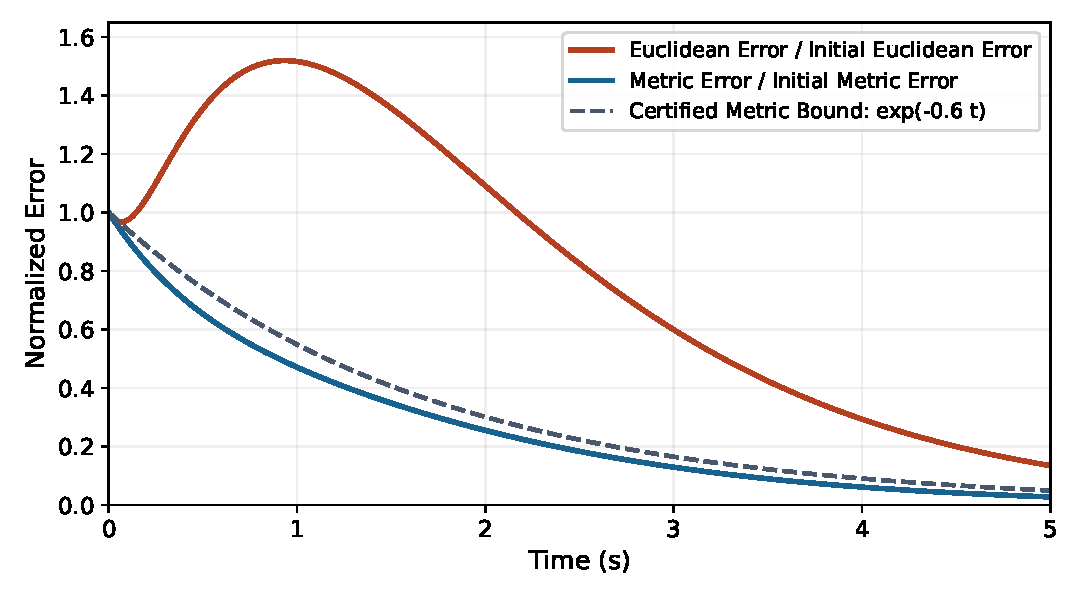
\includegraphics[width=0.88\linewidth]{../figures/contraction_cascade.pdf}
\caption{Transient Euclidean Growth and Certified Metric Decay for the Same Cascade. Each Norm Is Divided by Its Own Initial Value; the Metric Is $\operatorname{diag}(1,25)$.}
\label{fig:contraction_cascade}
\end{figure}

An illustrative cascade is
\begin{equation}
\dot q=-\alpha q+v,\qquad\dot v=-\gamma(v-u(t)),\qquad\alpha,\gamma>0.
\label{eq:ch4:mech-example}
\end{equation}
Here $v$ is an auxiliary driving state, not literally $\dot q$ when $\alpha\ne0$. Its cascade certificate needs the target-rate-dependent weight above. Setting $\alpha=0$ recovers the offset-preserving integrator, which cannot be uniformly exponentially contracting in a uniformly nondegenerate full-state metric. A mechanical linkage's kinematic ordering alone does not establish this triangular dynamical structure.

\section{Control Contraction Metrics: Design and Duality}
\label{sec:ch4:ccm}

\subsection{Feedback Design Under Contraction}

Consider
\begin{equation}
\dot x=f(x,t)+G(x,t)u,\qquad G=[g_1,\ldots,g_m].
\label{eq:ch4:controlled-system}
\end{equation}
The differential system is $\dot{\delta x}=A(x,u,t)\delta x+G\delta u$, with
$A=D_xf+\sum_i u_iD_xg_i$.
For a differential feedback $\delta u=-K(x,u,t)\delta x$,
\begin{equation}
A_{\mathrm{diff}}=A-GK.
\label{eq:ch4:closed-loop-jacobian}
\end{equation}
This is not the instruction $u=-K\delta x$ for a finite state. If a smooth implemented feedback is already known, use its actual derivative. Conversely, constructing a matrix field $K$ does not guarantee that it is the Jacobian of a single feedback function; integration along state-space paths provides a more general construction.

The differential feedback condition is
\begin{equation}
\dot M+(A-GK)^TM+M(A-GK)+2\lambda M\preceq0,
\label{eq:ch4:CCM-nonlinear}
\end{equation}
where $\dot M=\partial_tM+\partial_{f+Gu}M$. Both the input-dependent Jacobian and the metric's derivative along the controlled field are required.

\subsection{The Dual Formulation: Inverse Metric}

Differentiate $MW=I$ to obtain $\dot W=-W\dot MW$. Congruence of the preceding inequality by $W$, with $Y=KW$, gives
\begin{equation}
-\dot W+AW+WA^T-GY-Y^TG^T+2\lambda W\preceq0.
\label{eq:ch4:W-space-LMI}
\end{equation}
The derivative is $-\dot W$, the rate term is $+2\lambda W$, and the stabilizing input terms carry minus signs for our convention $\delta u=-K\delta x$. A source using $\delta u=K\delta x$ has the corresponding plus signs. A congruence preserves the matrix order, not its raw eigenvalues.

\subsection{Pointwise LMI for Feedback Synthesis}

For
\begin{equation}
\dot x=A(t)x+G(t)u,
\label{eq:ch4:LTV-system}
\end{equation}
one may choose $Y=\tfrac12\rho G^T$, obtaining
\begin{equation}
-\dot W+AW+WA^T-\rho GG^T+2\lambda W\preceq0,\qquad
K=\tfrac12\rho G^TW^{-1}.
\label{eq:ch4:pointwise-LMI}
\end{equation}
At fixed $\lambda$, this is linear in the unknown functions $W$ and $\rho$. It is a differential matrix inequality over time, not unrelated algebraic tests that may be solved independently at each instant. The multiplier $\rho$ creates feedback authority in actuated directions; it is not automatically a penalty or bound on physical effort.

For nonlinear systems, one useful sufficient construction imposes the stronger conditions
\begin{align}
-\partial_tW-\partial_fW+(D_xf)W+W(D_xf)^T
-\rho GG^T+2\lambda W&\prec0,\\
\partial_{g_i}W-(D_xg_i)W-W(D_xg_i)^T&=0\quad\text{for every }i.
\end{align}
The equalities cancel the terms proportional to arbitrary input values. Together with a smooth uniformly bounded positive metric and the complete-space/solution hypotheses, these conditions support the control contraction metric construction of Manchester and Slotine \cite{ManchesterSlotine2017}. They are sufficient conditions, not a claim that every stabilizable system must satisfy this particular parameterization.

The associated gain $K(x,t)=\tfrac12\rho(x,t)G(x,t)^TM(x,t)$ is independent of $u$. Given a feasible reference $(x_*,u_*)$ and a curve $c(s)$ joining $x_*$ to $x$, construct a path of controls by
$u(s)=u_*-\int_0^sK(c(r),t)c_r(r)\,dr$.
Transporting that curve with its controls, or recomputing suitable geodesics in a sampled/continuous construction under the theorem's conditions, converts differential contraction into finite tracking. Path existence, solution existence and controller regularity are part of the result. A domain restriction or an actuator limit must be incorporated explicitly; the unconstrained theorem does not certify saturation, muscle activation limits or unilateral ground contact.

\subsection{Computational Approaches}

For polynomial data, a domain certificate can require $M-\underline mI$ and the negative contraction residual to be positive-semidefinite through sum-of-squares representations, with suitable polynomial multipliers for the domain. The residual must include the desired $2\lambda M$ margin and all material derivatives. Such certificates are sufficient and may be conservative; failure of a selected polynomial degree does not prove that no smooth metric exists.

A neural parameterization may use $M=L(x,t)^TL(x,t)+\varepsilon I$, with $L\in\mathbb R^{p\times n}$ and $\varepsilon>0$. A vector-valued $L\in\mathbb R^p$ alone does not produce the required $n\times n$ matrix. A positive floor ensures positivity, but upper bounds and a certified contraction residual remain necessary. Optimizer convergence is not a proof of either.

Sampling is useful for finding and falsifying candidates. It is not automatically conservative between samples. For a symmetric residual $H$, suppose every point is within distance $h$ of a sample and a verified operator-norm Lipschitz constant is $L_H$. A sampled margin $\lambda_{\max}(H)\leq-\eta$ extends across that coverage only if $L_Hh<\eta$, with the region, boundaries, inputs and times all covered. This follows from the eigenvalue perturbation bound. Without such an argument, report sampled feasibility as sampled feasibility.

\section{Discrete-Time Contraction}
\label{sec:ch4:discrete}

\subsection{Discrete Contraction Condition}

Consider the actual implemented map
\begin{equation}
x_{k+1}=\Phi_k(x_k),\qquad J_k=D_x\Phi_k.
\label{eq:ch4:discrete-system}
\end{equation}
Assume the smooth map sends its certified path-connected domain into the next certified domain. A sequence of metrics satisfying
\begin{equation}
0<\underline mI\preceq M_k(x)\preceq\overline mI
\label{eq:ch4:discrete-metric-bounds}
\end{equation}
and
\begin{equation}
J_k(x)^TM_{k+1}(\Phi_k(x))J_k(x)\preceq\rho^2M_k(x),\qquad0<\rho<1,
\label{eq:ch4:discrete-contraction-condition}
\end{equation}
gives the following result.

\begin{theorem}[Discrete Distance Contraction]
\label{thm:ch4:discrete-contraction}
Under these domain and differential inequalities,
\begin{equation}
d_{M_k}(x_k^{(1)},x_k^{(2)})\leq\rho^k d_{M_0}(x_0^{(1)},x_0^{(2)}).
\label{eq:ch4:discrete-geodesic-decay}
\end{equation}
With a Euclidean-convex initial domain, the physical bound is
\begin{equation}
\|x_k^{(1)}-x_k^{(2)}\|\leq\sqrt{\overline m/\underline m}\,
\rho^k\|x_0^{(1)}-x_0^{(2)}\|.
\label{eq:ch4:discrete-euclidean-decay}
\end{equation}
\end{theorem}

To prove it, map an entire connecting curve: $c_{k+1}(s)=\Phi_k(c_k(s))$. Its tangent obeys $\partial_sc_{k+1}=J_k(c_k)\partial_sc_k$. The metric length shrinks by at least $\rho$; take infima and iterate. An arbitrary finite difference does not equal one endpoint Jacobian times the previous difference. Even $\Phi(x)=\tfrac12\tanh x$ illustrates this distinction while remaining globally contractive in the identity metric.

For sample period $\Delta t$, the equivalent length-decay rate is $-\log\rho/\Delta t$. An exact flow map of a continuously contracting system inherits the corresponding factor, but a numerical integrator need not. For $\dot x=-ax$, explicit Euler gives $1-a\Delta t$, which contracts only when $0<a\Delta t<2$. A digital controller must be checked as its actual sampled map, including held inputs and computation delays.

\subsection{Connection to Riccati Analysis}

For a stabilizing discrete LQR design, substitution into the Riccati equation gives
$A_c^TPA_c=P-Q-K^TRK$.
If $P\succ0$ and $Q+K^TRK\succeq(1-\rho^2)P$, this is a contraction certificate for the implemented closed loop. A semidefinite dissipation may require a multi-step argument instead of strict one-step decay. There is no universal theorem that contraction gives tighter guarantees than Riccati analysis; the latter can supply a particular metric, and both must be interpreted with their hypotheses and measured quantity.

\section{Numerical Example: Van der Pol Oscillator}
\label{sec:ch4:vdp}

\subsection{System Description}

The unforced Van der Pol system is
\begin{equation}
\dot x_1=x_2,\qquad\dot x_2=-x_1+\epsilon(1-x_1^2)x_2,\qquad\epsilon>0,
\label{eq:ch4:vdp-system}
\end{equation}
with
\begin{equation}
A=\begin{bmatrix}0&1\\-1-2\epsilon x_1x_2&\epsilon(1-x_1^2)\end{bmatrix}.
\label{eq:ch4:vdp-jacobian}
\end{equation}
No feedback input appears in this equation. It has an unstable equilibrium at the origin and an attracting nonconstant periodic orbit. Two solutions at different phases on that orbit cannot converge to each other at the same clock time. Full contraction on a domain containing the complete orbit is therefore impossible in a uniformly nondegenerate metric.

\subsection{Metric Synthesis via Parameterization}

For a diagonal candidate
\begin{equation}
M(x_1)=\operatorname{diag}(m_1(x_1),m_2(x_1)),
\label{eq:ch4:vdp-metric-ansatz}
\end{equation}
write $H=A^TM+MA+\dot M+2\lambda M$. Its entries are
\begin{align}
H_{11}&=m_1'(x_1)x_2+2\lambda m_1,\label{eq:ch4:vdp-cc-11}\\
H_{22}&=2\epsilon(1-x_1^2)m_2+m_2'(x_1)x_2+2\lambda m_2,\label{eq:ch4:vdp-cc-22}\\
H_{12}&=H_{21}=m_1+(-1-2\epsilon x_1x_2)m_2.\label{eq:ch4:vdp-cc-12}
\end{align}
The condition is $H\preceq0$, not componentwise inequalities on its off-diagonal entries. In two dimensions this requires $H_{11}\leq0$, $H_{22}\leq0$ and $\det H\geq0$. If $m_1$ is a positive constant, $H_{11}=2\lambda m_1>0$ for every positive requested rate. That alone disproves this entire candidate class for full contraction, at every point.

\subsection{Solution Strategy}

The formerly proposed example
\begin{equation}
M(x_1)=\operatorname{diag}\bigl(1,1.2(1+1.5x_1^2)\bigr),\quad
\epsilon=0.5,\quad\lambda=0.3
\label{eq:ch4:vdp-metric-solution}
\end{equation}
is retained only as a falsification exercise. At the origin its residual is
\begin{equation}
H(0)=\begin{bmatrix}0.6&-0.2\\-0.2&1.92\end{bmatrix}\not\preceq0.
\label{eq:ch4:vdp-check}
\end{equation}
Its velocity weight increases with $|x_1|$, not toward the origin. No successful optimizer or experimentally measured rate is claimed. The diagonal obstruction is stronger than a finite grid of violations.

The appropriate orbital question allows phase alignment. Transverse contraction tests decay only for nonzero tangent directions satisfying $\delta x^TMf=0$, with the associated field/metric derivatives and domain conditions. Manchester and Slotine's transverse framework \cite{ManchesterSlotineTransverse2013} requires a compact, smoothly path-connected, strictly forward-invariant set and appropriate regularity; an absence of equilibria distinguishes a nontrivial cycle from an equilibrium limit. It establishes convergence after a time reparameterization, not same-time tracking of a prescribed phase. We do not assert that the rejected diagonal candidate satisfies a transverse certificate.

A periodic orbit or multiple equilibria can obstruct a claimed global full-contraction domain. An invariant set of positive dimension by itself does not: the whole line is invariant under $\dot x=-x$ and the system contracts. An infeasible numerical search should be investigated using the actual obstruction, domain, metric class and solver residual.

\section{Robustness Margins From Contraction}

\subsection{Disturbance Attenuation via Contraction Rate}

First use a state-independent metric $M(t)$ to make the additive-disturbance claim precise. Compare the nominal $\dot x_0=f(x_0,t)$ with
\begin{equation}
\dot x_d=f(x_d,t)+d(t),\qquad\|d(t)\|\leq D.
\label{eq:ch4:perturbed-system}
\end{equation}
Assume both solutions and their connecting segments remain in a Euclidean-convex certified domain, the nominal Jacobian inequality holds throughout it, and the metric has the uniform bounds above. Integrating $f(x_d,t)-f(x_0,t)$ along the segment gives, for $r=\sqrt{(x_d-x_0)^TM(t)(x_d-x_0)}$, the upper derivative bound $D^+r\leq-\lambda r+\sqrt{\overline m}D$. It also holds at $r=0$ in the upper-derivative sense.

\begin{theorem}[Nominal-to-Perturbed Error Bound]
\label{thm:ch4:disturbance-rejection}
Under the preceding assumptions, with $\tau=t-t_0$,
\begin{equation}
\|x_d(t)-x_0(t)\|\leq\sqrt{\overline m/\underline m}\left[
e^{-\lambda\tau}\|x_d(t_0)-x_0(t_0)\|+
\frac{D}{\lambda}(1-e^{-\lambda\tau})\right].
\label{eq:ch4:ultimate-bound}
\end{equation}
Consequently, if the assumptions continue for all time,
\begin{equation}
\limsup_{t\to\infty}\|x_d(t)-x_0(t)\|\leq
\sqrt{\overline m/\underline m}\,D/\lambda.
\label{eq:ch4:ultimate-bound-steady}
\end{equation}
\end{theorem}

The proof is integration of the scalar comparison inequality, followed by the metric bounds. For two disturbed trajectories, replace $D$ by a bound on $\|d_1-d_2\|$, which may be $2D$ if each disturbance is separately bounded by $D$. A common additive disturbance cancels in the difference when the metric is state-independent. For a state-dependent metric, its material derivative changes with the disturbance; a nominal drift-only certificate does not automatically cover that change.

\subsection{Practical Implications}

Increasing a verified rate reduces this error bound when the forcing bound and metric comparison remain fixed. Controller changes can alter all three, including the disturbance generated by noisy measurements. A bounded error relative to a growing nominal trajectory is not a bounded state. Neither this inequality nor the contraction condition alone is a general guarantee that a stronger feedback gain is beneficial or feasible.

\section{Incremental Input-to-State Stability (ISS)}

\subsection{ISS vs. Contraction}

Input-to-state stability bounds the state by a decaying function of initial error and a gain of the input magnitude, relative to an appropriate zero-input equilibrium. Bounded-input/bounded-state behavior is only part of that statement. Incremental ISS instead bounds the difference between two solutions by their initial difference and input difference. Differential ISS is a tangent-level formulation; finite-distance conclusions require integration and geometry.

\begin{proposition}[A Uniform Input-Family Certificate]
\label{prop:ch4:contraction-iss}
For $\dot x=f(x,t)+G(x,t)u$, assume the contraction inequality, including $A=D_xf+\sum_i u_iD_xg_i$ and $\dot M=\partial_tM+\partial_{f+Gu}M$, holds uniformly for a convex admitted input set. Assume the input-interpolated trajectories and connecting curves stay in the certified domain, and $\|M^{1/2}G\|\leq\overline G_M$. Then
\begin{equation}
\|x_1(t)-x_2(t)\|\leq\sqrt{\overline m/\underline m}e^{-\lambda\tau}
\|x_1(t_0)-x_2(t_0)\|+
\frac{\overline G_M}{\lambda\sqrt{\underline m}}(1-e^{-\lambda\tau})
\sup_{s\in[t_0,t]}\|u_1(s)-u_2(s)\|,
\label{eq:ch4:diff-ISS-bound}
\end{equation}
provided the initial chord comparison is valid as above.
\end{proposition}

To see the input term, interpolate $u(s,t)=(1-s)u_1(t)+su_2(t)$ along a transported family. Its tangent dynamics acquire $G\partial_su$; Cauchy--Schwarz bounds the metric-length derivative by $-\lambda$ times length plus $\overline G_M\|u_2-u_1\|$. Integrate over the path and time. If only a Euclidean bound $\|G\|\leq\overline G$ is known, use $\overline G_M\leq\sqrt{\overline m}\,\overline G$. Omitting this metric factor changes the bound under a harmless rescaling of the ruler.

This proposition makes the required uniformity explicit. Contraction of one unforced field is not by itself incremental ISS of every controlled field. Ordinary ISS and contraction also have no unconditional implication ordering when their reference, input class and domains differ.

\section{Extended Lyapunov Comparison}

\subsection{Unified Perspective}

\begin{table}[htbp]
\centering\small
\begin{tabular}{@{}p{0.23\linewidth}p{0.68\linewidth}@{}}
\toprule
Property & What the Stated Property Establishes\\
\midrule
Lyapunov stability & Small initial errors remain small near the specified solution or set.\\
Asymptotic stability & Stability and eventual convergence; an exponential rate need not exist.\\
Exponential stability & A bound with a uniform exponential factor relative to the specified solution.\\
Incremental stability & A relationship between solution pairs, with the common inputs or differing inputs specified.\\
Contraction certificate & A differential metric inequality that integrates to pairwise convergence under the domain and metric assumptions.\\
\bottomrule
\end{tabular}
\caption{Distinct Stability Properties and Their Comparison Objects}
\label{tbl:ch4:lyapunov-contraction}
\end{table}

\subsection{Formal Relationships}

\begin{proposition}[An Equilibrium as the Comparison Solution]
\label{prop:ch4:contraction-lyapunov}
If an equilibrium $x_*$ lies in the forward-invariant contraction domain with the required metric/path bounds, using $x_2(t)=x_*$ gives exponential attraction and stability relative to that domain. A suitable finite-distance Lyapunov function is
\begin{equation}
\mathcal V(x,t)=d_{M,t}(x,x_*)^2,
\label{eq:ch4:induced-lyapunov}
\end{equation}
which decays at least as $e^{-2\lambda\tau}$. At nonsmooth distance points interpret the statement through the finite-time inequality or upper derivative.
\end{proposition}

In general $\mathcal V$ is not $(x-x_*)^TM(x)(x-x_*)$. For a concrete counterexample, let $z=\phi(x)=x+0.8\sin x$, so $0.2\leq\phi'(x)\leq1.8$, and define $\dot x=-\phi(x)/\phi'(x)$. In $z$ coordinates this is $\dot z=-z$, so $M(x)=\phi'(x)^2$ is a uniformly bounded contraction metric. The squared distance to zero is $\phi(x)^2$. The endpoint surrogate $x^2\phi'(x)^2$ has derivative
$2x\phi'(x)[\phi'(x)+x\phi''(x)]\dot x$, which is positive at $x=2$. The distinction is a real failure of the proposed Lyapunov argument, not a notational preference.

\section{Contraction in Biomechanical Systems}

\subsection{What Impedance Can Establish}

Mechanical impedance describes force response to motion; a contraction metric measures tangent-state error in a dynamical model. They are related through the equations of motion, but are different objects. Franklin and colleagues' arm-reaching experiment \cite{Franklin2003Stiffness} found direction-specific stiffness adaptation under unstable interactions, including changes not explained by altered net joint torque. This is evidence about an experimental task and measured mechanical response, not evidence that a golfer implements an optimal Riemannian metric.

Consider the explicitly simplified joint model
$I\ddot q+b\dot q+kq=\tau(t)$, with constant $I,b,k>0$ and a common torque input. For state $(q,v)$ its difference Jacobian is $A=[[0,1],[-k/I,-b/I]]$. This constant matrix is Hurwitz, so a positive solution of an appropriate Lyapunov equation supplies a full-state contraction metric. That is a model calculation; it does not require identifying the metric with muscle stiffness or joint inertia.

Mechanical error energy $E=\tfrac12(k\delta q^2+I\delta v^2)$ has derivative $\dot E=-b\delta v^2$. At nonzero position error and zero velocity error this derivative is zero, so this particular energy does not establish strict instantaneous contraction in every state direction. A different full-state metric can include position--velocity cross terms.

Nor does greater stiffness necessarily increase the asymptotic decay rate. In the underdamped constant model the eigenvalue real part is $-b/(2I)$, independent of $k$. Excessive damping can introduce a slow overdamped mode. Changing coactivation can alter stiffness, damping, activation state, metabolic cost and sensory response together; a verified comparison must use the resulting complete dynamics and admissible inputs.

Reflex delays require delayed-state or augmented-state analysis; they are not generally a static subtraction $GK$ that automatically improves a rate. Nonlinear muscle force--length--velocity relations, tendon compliance and state-dependent moment arms also change the Jacobian. The preceding two-state model is a transparent teaching example, not a complete neuromusculoskeletal certificate or a clinical prescription.

\subsection{Partial Contraction in Sequential Motion}

The torso--arm--club chain defines kinematic relationships. Its dynamics generally couple the links in both directions through the mass matrix, interaction forces and contact constraints. Applying a cascade theorem requires an actual triangular representation or a justified approximation with quantified residual coupling. Segment size, muscular strength and the order of speed peaks do not supply those hypotheses or their contraction rates.

Repeatable club delivery may coexist with substantial variation in redundant joint states. That motivates task-space or transverse questions rather than automatically demanding global contraction of every coordinate. However, a projected error that happens to shrink on measured trials is not yet a certificate for all perturbations: the hidden states can feed back into the output later.

\subsection{Contraction and the Drift-Dominated Phase}

Whether a phase is drift-dominated must be assessed in a specified model and with a declared comparison of accelerations, work or finite-horizon control authority. Rapid motion and large Coriolis terms do not by themselves establish negligible muscular influence. In a conservative passive model, energy and phase information can persist; inertial coupling redistributes motion without necessarily dissipating all perturbations.

For a specified policy and nominal swing, integrate $\dot\Phi=A_{\mathrm{cl}}(t)\Phi$, $\Phi(t_0)=I$. At a fixed terminal time, an output $y=h(x(t_f))$ has first-order sensitivity $\delta y=D h\,\Phi(t_f,t_0)\delta x_0$. This expression joins geometry, inertia, the torque/contact policy and the perturbation history. A contraction bound can upper-bound part of that map, but its usefulness depends on metric conditioning and output sensitivity. A merely contracting state metric does not optimize clubhead speed or ball-flight accuracy.

Impact is often state-triggered. Then the event-time derivative and reset/contact sensitivity enter the outcome map; a flow-only certificate need not survive the event. A useful research test specifies perturbation directions, measurement uncertainty, a feasible controller and an outcome such as clubface orientation or impact location, then compares predicted response bounds with held-out perturbations. Separate trials should retain their own noise and participant structure. This is a route to testing the robustness hypothesis, not a deduction of expert strategy from a sequence plot.

\section{Stochastic Contraction}

\subsection{Systems With Brownian Perturbations}

For an It\^o model
\begin{equation}
dx=f(x,t)\,dt+\sigma(x,t)\,dW_t,
\label{eq:ch4:sde}
\end{equation}
state which noise is shared between the compared solutions. A common-noise comparison asks whether different initial states synchronize under the same random forcing. Independent-trial repeatability is a different quantity. Pham, Tabareau and Slotine \cite{PhamTabuadaSlotine2009} explicitly analyze independent Wiener processes using state-independent metrics and a bounded diffusion trace.

\subsection{The Stochastic Contraction Condition}

The following state-independent-metric version has an elementary generator proof. Assume well-posed solutions with the integrability needed for It\^o's formula and finite second moments, initial states independent of future noise, a common metric $M(t)$ with uniform positive bounds, and the deterministic contraction inequality globally. Suppose
$\operatorname{tr}(\sigma(x,t)^TM(t)\sigma(x,t))\leq C$
uniformly. Compare two solutions driven by independent Wiener processes and set $V=(x_1-x_2)^TM(t)(x_1-x_2)$.

\begin{theorem}[Independent-Noise Mean-Square Bound]
\label{thm:ch4:stochastic-contraction}
With $\tau=t-t_0$, the preceding assumptions imply
\begin{equation}
\mathbb E[V(t)]\leq e^{-2\lambda\tau}\mathbb E[V(t_0)]
+\frac{C}{\lambda}(1-e^{-2\lambda\tau}).
\label{eq:ch4:stochastic-bound}
\end{equation}
\end{theorem}

The drift contribution is at most $-2\lambda V$, by the same segment argument used for deterministic forcing. It\^o's formula adds two diffusion traces, one for each independent solution, totaling at most $2C$. Thus $\frac{d}{dt}\mathbb E V\leq-2\lambda\mathbb E V+2C$ and scalar integration proves the claim. A general state-dependent metric introduces additional stochastic derivative terms and needs a separate theorem; the deterministic material derivative is not enough.

\subsection{Connection to Uncertainty Propagation}

For the scalar Ornstein--Uhlenbeck process $dx=-ax\,dt+\sigma\,dW$, $a>0$, the solution is
$x(t)=e^{-a\tau}x(t_0)+\sigma\int_{t_0}^te^{-a(t-s)}dW_s$.
The It\^o isometry gives three distinct conclusions:
\begin{itemize}
\item One trial with deterministic initial state has variance $\sigma^2(1-e^{-2a\tau})/(2a)$ and stationary variance $\sigma^2/(2a)$.
\item Two independent trials have mean-square difference $e^{-2a\tau}\mathbb E[(x_1(t_0)-x_2(t_0))^2]+\sigma^2(1-e^{-2a\tau})/a$.
\item With the same additive noise realization, the difference is exactly $e^{-a\tau}(x_1(t_0)-x_2(t_0))$; the noise cancels and there is no pairwise additive floor.
\end{itemize}
These statements do not extend unchanged to multiplicative common noise. For $dx=-ax\,dt+bx\,dW$, the mean-square difference under common noise evolves as $e^{(-2a+b^2)\tau}\mathbb E[\delta x(t_0)^2]$. It grows when $b^2>2a$, even though the deterministic drift contracts.

From the metric bound, an asymptotic upper bound on root-mean-square Euclidean separation is $\sqrt{C/(\lambda\underline m)}$. Expected distance is no larger than RMS distance by Jensen's inequality, but need not equal it or attain this upper bound. An observer claim additionally needs its actual error dynamics, sensor noise and observability assumptions. There is no blanket guarantee that a contracting observer outperforms an extended Kalman filter, or that increasing feedback lowers noise-driven error when the gain itself injects measurement noise.

\section{Contraction Tubes and Funnel Control}

\subsection{The Contraction Tube}

For a feasible nominal solution $\bar x(t)$, define
\begin{equation}
\mathcal T_r(t)=\{x\in\mathcal D:d_{M,t}(x,\bar x(t))\leq r\}.
\label{eq:ch4:tube}
\end{equation}
With certified scalar comparison $D^+d_{M,t}\leq-\lambda d_{M,t}+d$, the radius
\begin{equation}
r(t)=r_0e^{-\lambda\tau}+\frac d\lambda(1-e^{-\lambda\tau})
\end{equation}
bounds solutions beginning in $\mathcal T_{r_0}(t_0)$, while the entire tube stays inside the certified domain. It starts at $r_0$ and approaches $d/\lambda$. With $d=0$ it shrinks exponentially. Here $d$ is a bound on forcing in metric-length units, not automatically the raw magnitude of torque or a Euclidean disturbance.

If $M$ is state-independent, these metric balls are ellipsoids in the chosen coordinates, with semi-axis lengths $r/\sqrt{\mu_i(M)}$. A state-dependent metric generally gives curved distance balls. Its endpoint matrix describes a local approximation, not an exact global ellipsoid. A condition number describes relative axis shape; absolute scale and the selected radius determine size.

\subsection{Funnel Control}

A prescribed positive boundary $\varphi(t)$ can contain a contracting distance when the initial distance is inside it and
$\dot\varphi(t)+\lambda\varphi(t)\geq d$.
At a potential first boundary crossing this condition makes the outward distance derivative no larger than the boundary derivative. In the unforced case it reduces to $\lambda\geq-\dot\varphi/\varphi$. Strict containment needs an appropriate strict initial margin and regularity; the tube and control must remain feasible throughout.

This comparison is not a general funnel-controller design theorem. A gain that diverges near a boundary may violate torque, activation, contact or sampling limits and may not be suitable for the plant's relative degree or internal dynamics. A certified funnel in a golf model must include those restrictions. Its radius at impact can bound a specified state error, but a bound on ball flight requires the separate impact/output map and its uncertainty.

\section{Reproducible Numerical Checks}

The following program runs from the repository root with NumPy and SciPy. The helper reports a signed pointwise rate; it does not search for or certify a metric over a domain.
\begin{lstlisting}[language=Python]
import numpy as np
from scipy.linalg import solve_continuous_lyapunov
from src.tools.contraction_examples import (
    local_contraction_rate, vdp_candidate_residual,
)

A = np.array([[-2.0, 1.0], [0.0, -3.0]])
M = solve_continuous_lyapunov(A.T, -np.eye(2))
zero = np.zeros((2, 2))
print(local_contraction_rate(A, np.eye(2), zero))
print(M)
print(local_contraction_rate(A, M, zero))

cascade = np.array([[-1.0, 4.0], [0.0, -1.0]])
print(local_contraction_rate(cascade, np.diag([1.0, 25.0]), zero))
print(vdp_candidate_residual(np.zeros(2)))
\end{lstlisting}
The outputs are the identity rate approximately $1.792893$, the Lyapunov metric given above, its generalized rate $30/(13+\sqrt{13})$, the cascade rate $0.6$, and the rejected Van der Pol residual $[[0.6,-0.2],[-0.2,1.92]]$. Independent checks compare metric decay with exact matrix exponentials, differentiate the nonlinear field and candidate metric numerically, verify the dual congruence, integrate the OU variance and tube forcing, and construct the endpoint-distance counterexample. These calculations test the displayed mathematics; they are not simulated or measured golfer performance.

\section{Chapter Summary}

Contraction turns a differential metric inequality into a finite-distance bound by transporting connecting curves. Its interpretation depends on the complete vector field, common comparison clock, domain, metric scales and input assumptions. Matrix order, total derivatives and length-versus-squared-length factors are essential parts of the argument.

A cascade needs controlled coupling as well as contracting blocks. A CCM needs a finite controller construction as well as a differential gain. A sampled residual needs a between-sample certificate; a discrete controller needs a certificate for its actual map. Orbital convergence, independent-trial repeatability and same-time full-state convergence answer different questions.

For the golf swing, the productive connection is to specify a physical model and feasible policy, propagate meaningful perturbations, and connect the result to delivery and impact. Impedance measurements and repeatable motion can inform that investigation. They do not remove the need to establish the mathematical hypotheses or validate the resulting predictions.

\section{Further Reading}

Lohmiller and Slotine \cite{LohmillerSlotine1998} provide the foundational differential treatment. Manchester and Slotine \cite{ManchesterSlotine2017} develop control contraction metrics and the path-based controller construction; their transverse paper \cite{ManchesterSlotineTransverse2013} treats orbital rather than same-time convergence. Pham, Tabareau and Slotine \cite{PhamTabuadaSlotine2009} state the noise independence and metric restrictions behind their stochastic result. Franklin and colleagues \cite{Franklin2003Stiffness} provide a specific reaching experiment on stiffness adaptation, whose measured scope should be distinguished from a contraction certificate for golf.

\section*{Exercises}

\begin{enumerate}
\item \textbf{Contraction of a Linear System.} For $A=[[-1,2],[0,-3]]$, compute the identity-metric rate. For $M=\operatorname{diag}(1,\theta)$, derive $\lambda(\theta)=2-\sqrt{1+1/\theta}$. Find the weights giving a prescribed rate below one, and explain why the supremum one is not attained by any finite positive diagonal weight. Compare with a nondiagonal metric constructed from eigenvectors.
\item \textbf{LMI Feasibility on a Domain.} For $\dot x_1=-x_1+x_2^2$, $\dot x_2=-2x_2+u$, apply $u=-x_2$. Show that no constant positive metric certifies a fixed positive rate on all $\mathbb R^2$: the unbounded off-diagonal coupling must be addressed. On the invariant strip $|x_2|\leq R$, use $M=\operatorname{diag}(1,\theta)$ and derive a sufficient weight for any $0<\lambda<1$.
\item \textbf{Partial and Cascade Contraction.} For the same cascade with $|u(t)|\leq U$, show that $|x_2|\leq R$ is invariant when $2R\geq U$. Bound the coupling there and find a weighted full-state certificate for a target rate below one. Explain why a statement based only on the two diagonal subsystem rates is insufficient, and contrast it with the position integrator $\dot q=v$.
\item \textbf{From Differential to Finite Feedback.} For $\dot x_1=x_2$, $\dot x_2=-x_1^3+u$, use $u=x_1^3-k_px_1-k_dx_2$ with $k_p,k_d>0$ to obtain a linear stable closed loop. Solve its Lyapunov equation and compute $K=-D_xu$ for our differential sign convention. Verify the primal and dual identities. Explain why an arbitrary polynomial differential gain would still require a finite controller construction and an actuator-feasibility check.
\item \textbf{Discrete-Time Contraction.} For $x_{k+1}=Ax_k$, show that a constant positive metric with induced norm $\|A\|_M<1$ exists precisely when $A$ is Schur stable. Give the length factor and its equivalent continuous-time rate for sample period $\Delta t$. Compare an exact scalar stable flow with explicit Euler and find the latter's allowable step interval.
\item \textbf{Stochastic Comparisons.} Derive the finite-time and stationary variances for $dx=-ax\,dt+\sigma\,dW$. Compute the mean-square difference for common-noise and independent-noise pairs, retaining the initial difference. Then derive the common-noise multiplicative condition $b^2<2a$ for mean-square decay in $dx=-ax\,dt+bx\,dW$.
\item \textbf{Tube Computation.} Use the identity rate of Exercise1, metric forcing bound $d=0.1$ and $r_0=1$. Compute the exact scalar comparison radius and the time at which it reaches twice its asymptotic radius, checking that such a positive time exists. Derive the inequality on a prescribed boundary $\varphi(t)$ and state the required initial/domain assumptions.
\item \textbf{Mechanical Impedance and Contraction.} For $I\ddot q+b\dot q+kq=\tau(t)$ with positive constants and common torque input, derive the two-state Jacobian and a full-state Lyapunov metric. Explain why the mechanical error energy has only semidefinite dissipation and why increasing stiffness need not increase the decay rate. State what additional dynamics and measurements would be required before using this model to interpret coactivation during a golf swing.
\end{enumerate}

%% Canonical manuscript; keep the Quarto chapter synchronized.
\chapter{Local Optimal Control: LQR, DDP, and Riccati}
\label{ch:optimal-control}

\begin{laymansbox}{Zoom in, Solve, Check, Repeat}{zoom_in_solve}
A motion planner needs both a destination and a price for getting there. It
predicts how today's action affects later states, then balances the predicted
benefit against effort and other costs. For a linear system with a quadratic
objective, this calculation is exact. For a nonlinear system it is a local
approximation: roll the proposed action through the full dynamics and check
whether the promised improvement actually occurs.
\end{laymansbox}

Three questions organize this chapter: what is optimal for a specified model
and cost, whether an algorithm finds a stationary solution, and whether the
resulting feedback stabilizes the physical system. An answer to one does not
automatically answer the others.

\section{Bellman and Pontryagin: Two Views of the Same Objective}

For a fixed initial state, consider
\begin{equation}
\min_{u_0,\ldots,u_{N-1}}J=\ell_N(x_N)+\sum_{k=0}^{N-1}\ell_k(x_k,u_k),
\qquad x_{k+1}=f_k(x_k,u_k).
\label{eq:ch5:traj-opt}
\end{equation}
Here $x_k\in\mathbb R^n$, $u_k\in\mathbb R^m$, and $f_k$ is a discrete
transition, potentially obtained by integrating a continuous model. Its
derivatives must match that transition and its time step.

Bellman's principle gives
\begin{equation}
V_k(x)=\min_u\{\ell_k(x,u)+V_{k+1}(f_k(x,u))\},\qquad V_N=\ell_N.
\label{eq:ch5:bellman}
\end{equation}
The future value makes this different from repeatedly minimizing today's stage
cost. With linear dynamics, quadratic costs, and unconstrained controls, this
recursion reduces to a Riccati recursion~\cite{bellman1957}.

For Pontryagin's conditions, choose the Lagrangian sign convention
\begin{equation}
\mathcal L=\ell_N(x_N)+\sum_{k=0}^{N-1}
\{\ell_k(x_k,u_k)+\lambda_{k+1}^{T}[f_k(x_k,u_k)-x_{k+1}]\}.
\label{eq:ch5:lagrangian}
\end{equation}
With $H_k=\ell_k+\lambda_{k+1}^{T}f_k$, stationarity gives
\begin{align}
0&=\ell_{k,u}+f_{k,u}^{T}\lambda_{k+1},\label{eq:ch5:kkt-u}\\
\lambda_k&=\ell_{k,x}+f_{k,x}^{T}\lambda_{k+1},\quad
\lambda_N=\ell_{N,x}.\label{eq:ch5:costate-update}
\end{align}
In continuous time, the normal minimization convention $H=L+\lambda^Tf$
uses $\dot x=H_\lambda$, $\dot\lambda=-H_x$, and a control minimizing $H$.
The alternative maximum convention changes the sign of the running-cost term.
The name ``maximum principle'' does not justify mixing conventions. For
general discrete nonlinear dynamics the displayed stationarity conditions are
necessary first-order conditions; they do not establish a global Hamiltonian
minimum~\cite{pontryagin1962}.

Where the value function is differentiable, the costate trajectory is the
gradient of the value function along an optimal trajectory:
$\lambda_k=\nabla_xV_k(x_k)$. Thus $V=\tfrac12x^TSx$ gives $\lambda=Sx$,
whereas $V=x^TSx$ gives $\lambda=2Sx$. A costate is a covector of marginal
cost, not the scalar cost itself. Constraints, nondifferentiable values, and
abnormal extremals require the corresponding more general conditions.

\section{A Dimensionally Consistent Local Model}

For the Taylor models below, assume the transition and stage/terminal costs
are twice continuously differentiable near the feasible nominal trajectory.
Use independent local coordinates for state perturbations. If a transition
includes an impact, a fixed-mode flow Jacobian alone omits the reset and
event-time sensitivity. This smooth derivation does not supply those event
derivatives; a hybrid transition requires its own applicable treatment
\cite{Kong2024SaltationFoundations}.

Let $(\bar x_k,\bar u_k)$ be dynamically feasible and write
$\delta x=x-\bar x$, $\delta u=u-\bar u$. Derivatives below are evaluated
on that trajectory. Use column gradients,
$\ell_{ux}\in\mathbb R^{m\times n}$, and $\ell_{xu}=\ell_{ux}^T$:
\begin{equation}
\ell\simeq\ell_0+\ell_x^T\delta x+\ell_u^T\delta u+
\frac12\begin{bmatrix}\delta x\\\delta u\end{bmatrix}^{T}
\begin{bmatrix}\ell_{xx}&\ell_{xu}\\\ell_{ux}&\ell_{uu}\end{bmatrix}
\begin{bmatrix}\delta x\\\delta u\end{bmatrix}.
\label{eq:ch5:cost-expansion}
\end{equation}
Retain the linear terms: they drive improvement when the nominal trajectory
is not stationary. Dropping them generally removes the feedforward correction.
The first-order dynamics are
\begin{equation}
\delta x_{k+1}\simeq A_k\delta x_k+B_k\delta u_k,
\qquad A_k=f_{k,x},\quad B_k=f_{k,u}.
\label{eq:ch5:perturbation}
\end{equation}
Even an exact Jacobian gives a tangent approximation to a finite perturbation.
An infeasible nominal trajectory introduces a defect
$f_k(\bar x_k,\bar u_k)-\bar x_{k+1}$ that a defect-aware method must carry.

Write the next local value as
$V_{k+1}\simeq V_0+s^T\delta x_{k+1}+\tfrac12\delta x_{k+1}^TS\delta x_{k+1}$.
The action value $Q=\ell+V_{k+1}\circ f_k$ has derivatives
\begin{align}
Q_x&=\ell_x+A^Ts,&Q_u&=\ell_u+B^Ts,\label{eq:ch5:Qx}\\
Q_{xx}&=\ell_{xx}+A^TSA+\sum_i s_i f^i_{xx},\label{eq:ch5:Qxx}\\
Q_{uu}&=\ell_{uu}+B^TSB+\sum_i s_i f^i_{uu},\label{eq:ch5:Quu}\\
Q_{ux}&=\ell_{ux}+B^TSA+\sum_i s_i f^i_{ux}.\label{eq:ch5:Qxu}
\end{align}
The superscript $i$ selects a component of $f$. The sums contract the value
gradient with dynamics second derivatives. Full DDP retains these terms;
iLQR omits them. Both methods retain the complete cost Hessian, including
$\ell_{ux}$, and the first-derivative coupling $B^TSA$. Velocity dependence
does not itself require full DDP: iLQR still linearizes those dynamics.

\section{The Discrete Riccati Recursion}

Suppose $Q_{uu}\succ0$. Invertibility alone gives only a stationary control,
possibly a maximum or saddle. Completing the square gives
\begin{align}
\delta u^*&=k+K\delta x,\label{eq:ch5:feedback-affine}\\
k&=-Q_{uu}^{-1}Q_u,&K&=-Q_{uu}^{-1}Q_{ux}.\label{eq:ch5:gain-def}
\end{align}
Negative signs are included in $k$ and $K$ throughout this chapter. Implement
the inverses with factorization and linear solves. The unregularized update is
\begin{align}
s_k&=Q_x-Q_{xu}Q_{uu}^{-1}Q_u,\\
S_k&=Q_{xx}-Q_{xu}Q_{uu}^{-1}Q_{ux}.\label{eq:ch5:S-def}
\end{align}
Initialize $s_N=\ell_{N,x}$ and $S_N=\ell_{N,xx}$. Both gradient and
curvature must be propagated. A large eigenvalue of $Q_{uu}$ penalizes a
control change; for fixed gradient it reduces the step in that direction.

For linear dynamics and stage cost
$\ell_k=\tfrac12(x^TQ_kx+2u^TN_kx+u^TR_ku)$, with
$N_k\in\mathbb R^{m\times n}$, the exact recursion is
\begin{align}
H_k&=R_k+B_k^TS_{k+1}B_k,\quad D_k=N_k+B_k^TS_{k+1}A_k,\\
K_k&=-H_k^{-1}D_k,\\
S_k&=Q_k+A_k^TS_{k+1}A_k-D_k^TH_k^{-1}D_k,\quad S_N=Q_N.
\label{eq:ch5:riccati-full}
\end{align}
A sufficient convexity assumption is that the joint stage-cost block
$\left[\begin{smallmatrix}Q_k&N_k^T\\N_k&R_k\end{smallmatrix}\right]$
is positive semidefinite, $R_k\succ0$, and $Q_N\succeq0$. For $N_k=0$
this is the familiar $Q_k\succeq0$, $R_k\succ0$ setting. The feedback
minimizes this finite-horizon linear-quadratic problem globally. Applying it
to a nonlinear system has a local approximation scope.

An independent check, including the cross-cost terms, is
\begin{equation}
S_k=Q_k+K_k^TN_k+N_k^TK_k+K_k^TR_kK_k+
(A_k+B_kK_k)^TS_{k+1}(A_k+B_kK_k).
\label{eq:ch5:riccati-alt}
\end{equation}
Let $A=B=Q=R=1$, $N=1/2$, and $S_{k+1}=1$. Then
$H=2$, $D=3/2$, $K=-3/4$, and $S_k=7/8$. Both formulas give $7/8$;
omitting the two cross-cost terms does not.

\section{Controllability, Finite Cost, and Stabilization}

Finite-horizon LQR does not require controllability. Under the positivity
assumptions above, $H_k\succ0$, including when $B_k=0$. The optimizer then
computes unavoidable state cost. Controllability asks whether arbitrary state
transfers can be achieved. A hard terminal equality can be infeasible even
though unconstrained finite-horizon LQR has a finite solution.

For a continuous time-varying linearization, endpoint reachability uses
\begin{equation}
W_c(t_0,T)=\int_{t_0}^T\Phi(T,s)B(s)B(s)^T\Phi(T,s)^T\,ds,
\end{equation}
where $\Phi$ is the state-transition matrix of $A(t)$. A frozen-time rank
test on $[B,AB,\ldots]$ is not a general substitute. Small Gramian eigenvalues
indicate expensive transfers under the specified state units and input metric;
raw condition numbers change under arbitrary rescaling.

For infinite-horizon time-invariant LQR with $Q\succeq0$, $R\succ0$, and
no cross term, stabilizability of $(A,B)$ and detectability of $(Q^{1/2},A)$
are standard sufficient assumptions for the stabilizing Riccati solution.
Controllability is stronger than necessary. A finite-horizon optimum alone
does not guarantee asymptotic stability.

\section{Differential Dynamic Programming and iLQR}
\label{sec:ch5:ilqr-vs-ddp}

DDP repeatedly constructs the local action value and updates the nominal
trajectory~\cite{jacobson1970dpp}. A practical implementation follows this sequence.
\begin{enumerate}
\item Specify initial state, model, integration method, horizon, cost, and
constraints. Roll out nominal controls to obtain a feasible state sequence.
\item Compute cost gradients and Hessians and dynamics derivatives. Full DDP
adds the three dynamics-Hessian contractions; iLQR omits those contractions.
\item Sweep backward from the terminal gradient and Hessian. Ensure positive
control curvature, increasing regularization and restarting when necessary.
\item From the same initial state, roll out
$u_k^{\rm trial}=\bar u_k+\alpha k_k+K_k(x_k^{\rm trial}-\bar x_k)$ and
$x_{k+1}^{\rm trial}=f_k(x_k^{\rm trial},u_k^{\rm trial})$.
\item Compare actual and predicted cost changes and accept sufficient decrease.
If no trial is acceptable, increase regularization or report failure.
\item Check stationarity, feasibility, cost change, and step size. A failed
line search or tiny regularized step is not a certificate of convergence.
\end{enumerate}

Here $\alpha$ is a trial step fraction, $0<\alpha\le1$. It scales the
feedforward correction; the feedback term uses the trial trajectory's state
deviation. Test the resulting rollout against the original objective.

When choosing a policy, regularization may replace $Q_{uu}$ by $Q_{uu}+\mu I$.
Choose $\mu$ large enough to obtain positive definiteness. To evaluate that
policy in the original quadratic model, use general substitution:
\begin{align}
s_k&=Q_x+K^TQ_u+Q_{xu}k+K^TQ_{uu}k,\\
S_k&=Q_{xx}+Q_{xu}K+K^TQ_{ux}+K^TQ_{uu}K.
\end{align}
Mixing regularized gains with an unqualified Schur-complement update silently
changes the model. State the regularization convention implemented.

Identity regularization uses a declared control scale. For inputs with
different units or characteristic magnitudes, normalize the controls or specify
a fixed positive-definite regularization metric $W$. Choose $\mu W$ with units
compatible with $Q_{uu}$; the added quadratic penalty is
$\tfrac{\mu}{2}\delta u^TW\delta u$, with $\mu\ge0$.
Under a constant nonsingular change of scale $\delta u=T_u\delta v$,
\begin{equation}
\begin{aligned}
H_{\rm reg}&=Q_{uu}+\mu W,\\
H_{{\rm reg},v}&=T_u^TQ_{uu}T_u+\mu T_u^TWT_u.
\end{aligned}
\label{eq:ch5:regularization-scale}
\end{equation}
The metric transforms by congruence. Replacing $T_u^TWT_u$ by an identity
matrix generally changes the physical trial policy. The original $\mu I$
rule is valid in its declared scale; it is not invariant to arbitrary input
rescaling. Numerical regularization is not a measurement of mechanical joint
damping or metabolic expenditure.

Both methods use local Taylor approximations. Solving a quadratic subproblem
exactly does not make that approximation globally exact or establish a global
optimum. Repeated relinearization updates the approximation where it is used.
For dense matrices, both methods propagate an $n\times n$ value Hessian and
factor an $m\times m$ control Hessian. Standard dense algebra costs on the
order of $N(n^3+n^2m+nm^2+m^3)$, before derivative evaluation. Full DDP adds
dynamics second derivatives or their contractions. iLQR does not reduce the
whole backward pass to $O(Nm^3)$. Compare measured runtime at matched
tolerances; there is no universal hundredfold speed advantage.

\section{What Local Convergence Requires}
\label{sec:ch5:ddp-as-newton}

Eliminating states in an unconstrained shooting problem yields a reduced
objective $J(U)$ in stacked controls. Exact Newton solves
$\nabla^2J(U)\Delta U=-\nabla J(U)$. With positive-definite Hessian at a
stationary point, locally Lipschitz Hessian, sufficiently close initialization,
and eventual full unregularized steps, its standard local result is
\begin{equation}
\|U^{(i+1)}-U^*\|\le C\|U^{(i)}-U^*\|^2.
\label{eq:ch5:quad-convergence}
\end{equation}
This measures error from the solution, not successive step size. A strict
minimum need not have a positive-definite Hessian; twice continuous
differentiability alone does not imply a Lipschitz Hessian.

Full second-order DDP has a closely related local quadratic-convergence theory
under suitable smoothness, nonsingular positive control curvature, and step
acceptance assumptions~\cite{jacobson1970dpp}. Its nonlinear feedback rollout
need not equal an open-loop Newton step away from the solution. Holding each
costate fixed and independently minimizing its Hamiltonian misses the dependence
of later states and costates on that control.

iLQR uses an approximate reduced Hessian. Superlinear convergence is not a
general consequence: linear convergence is possible, and faster rates need
additional conditions on omitted terms. An exact Jacobian alone establishes
neither quadratic nor global convergence. Globalization helps find acceptable
steps without guaranteeing the desired local minimum.

\section{A Reproducible Pendulum Example}

For a point mass $m$ on a massless rod of length $l$, viscous damping $b\ge0$,
torque $\tau$, and angle measured from downward vertical,
\begin{equation}
ml^2\ddot\theta=-mgl\sin\theta-b\dot\theta+\tau.
\label{eq:ch5:pendulum-dynamics}
\end{equation}
Hanging is $\theta=0$ and upright is $\theta=\pi$. With $m=1\,\mathrm{kg}$,
$l=1\,\mathrm m$, $g=10\,\mathrm{m/s^2}$, $b=0.1\,\mathrm{N\,m\,s}$,
\begin{equation}
\dot\theta=\omega,\qquad\dot\omega=-10\sin\theta-0.1\omega+\tau.
\label{eq:ch5:pendulum-first-order}
\end{equation}
The energy $E=\tfrac12ml^2\omega^2+mgl(1-\cos\theta)$ obeys
$\dot E=\tau\omega-b\omega^2$, independently checking the damping sign.

A swing-up angle penalty $1+\cos\theta$ is minimized at upright. An illustrative
running cost is $L=1+\cos\theta+0.1\omega^2+0.01\tau^2$.
Near upright, an unwrapped local angle chart allows the balancing cost
$100(\theta-\pi)^2+10\omega^2+0.1\tau^2$.
These weighted objectives are not energy or metabolic expenditure. A step $h$
gives a running-cost approximation $hL$; changing $h$ without scaling it changes
the trade-off with terminal cost.

An independently reproducible calculation is infinite-horizon LQR balance for
$e=\theta-\pi$ with
\begin{equation}
A=\begin{bmatrix}0&1\\10&-0.1\end{bmatrix},\quad
B=\begin{bmatrix}0\\1\end{bmatrix},\quad Q=\operatorname{diag}(100,10),\quad R=0.1.
\end{equation}
For cost $\int_0^\infty(x^TQx+R\tau^2)dt$, feedback is
$\tau=-R^{-1}B^TPx$. Write the symmetric $P$ using entries
$p_{11},p_{12},p_{22}$. Its stabilizing solution satisfies
\begin{align}
p_{12}&=1+\sqrt{11},\\
p_{22}&=\frac{-0.2+\sqrt{0.04+40(2p_{12}+10)}}{20},\\
p_{11}&=0.1p_{12}-10p_{22}+10p_{12}p_{22}.
\end{align}
The position and velocity feedback gains are approximately $43.166$ and
$13.551$. The closed-loop polynomial is
$s^2+(0.1+13.551)s+(43.166-10)$, with negative real-part roots. This establishes
linearized local balance, not swing-up or robustness to arbitrary torque limits.

To report a swing-up experiment, publish initial state, integration scheme and
step, horizon, bounds, objective, initial controls, solver version, derivative
checks, stopping tolerances, and trajectories. Check energy residuals and step
convergence. The previous iteration and gain tables did not specify such a
reproducible run; they are not evidence for the corrected model.

\section{Constraints and the Meaning of the Cost}

Clamping a trial torque respects box bounds for that trial but does not solve
the bound-constrained local problem. Use a box-constrained backward solve or
another constrained optimizer. Augmented Lagrangian methods update multipliers
as well as penalties; a pure penalty method should not be given that name.

A soft penalty $\rho\max(0,g(x))^2/2$ does not guarantee $g(x)\le0$ at finite
$\rho$. A logarithmic barrier $-\mu\log[-g(x)]$, $\mu>0$, tends to positive
infinity when approaching the boundary from inside. It is undefined outside,
so the solver must reject infeasible trials. Neither treatment automatically
enforces constraints between integration nodes.

Weights encode the question. Normalize by meaningful scales and distinguish
impact accuracy, peak load, squared torque, work, and metabolic cost. Squared
torque and work have different dimensions and favor different actions. Examine
sensitivity to weights. Increasing an effort weight is not a universal method
for increasing damping: check poles, constraints, and nonlinear response.

\section{Continuous-Time Riccati and a Counterexample}

The Hamilton--Jacobi--Bellman equation is
\begin{equation}
-V_t=\min_u\{L+\nabla V^Tf\},\qquad V(T,x)=\ell_T(x).
\label{eq:ch5:hjb}
\end{equation}
For $\dot x=Ax+Bu$, $L=\tfrac12(x^TQx+u^TRu)$, and $V=\tfrac12x^TSx$,
\begin{equation}
-\dot S=Q+A^TS+SA-SBR^{-1}B^TS,\quad S(T)=Q_T,\quad u^*=-R^{-1}B^TSx.
\label{eq:ch5:DRE}
\end{equation}
The time-invariant algebraic equation sets $\dot S=0$ and requires the
stabilizing solution under the assumptions stated earlier.
For $\dot x=x$, $B=0$, $Q=1$, $Q_T=0$, the finite-horizon solution is
$S(t)=(e^{2(T-t)}-1)/2$. It is finite despite uncontrollability and instability.
The infinite-horizon cost diverges for nonzero initial state. Finite cost,
reachability, and stabilization are different properties.

\section{Model Predictive Control and Terminal Guarantees}

MPC repeatedly solves a finite-horizon problem from the measured state,
applies its first control, and replans. DDP and iLQR are possible solvers,
alongside other nonlinear and quadratic-programming methods. Warm-start by
shifting old controls one relative horizon index, appending terminal control,
and rolling out states from the new measurement. Disturbances and changing
active constraints can make this guess poor.

A standard nominal stability argument assumes admissible terminal feedback
$\kappa_f$, an invariant terminal set $\mathcal X_f$, and
\begin{equation}
V_f(f(x,\kappa_f(x)))-V_f(x)\le-\ell(x,\kappa_f(x)),\qquad x\in\mathcal X_f.
\end{equation}
With initial feasibility, the terminal constraint, positive-definite stage
cost relative to the target, and appropriate regularity, a shifted candidate
establishes recursive feasibility and decrease of the optimal value. Exact
optimization, or a suboptimal solver preserving that feasibility and decrease,
supports the stability conclusion. An arbitrary finite-horizon local solve
does not supply those guarantees.

An LQR quadratic is a candidate terminal cost; nonlinear decrease and input
admissibility must be checked on the terminal set. Lyapunov decrease toward
one equilibrium differs from contraction between trajectories. A differential
metric $M(x,t)$ needs uniform positive-definiteness bounds and an inequality
involving $\dot M+A_{\rm cl}^TM+MA_{\rm cl}$ throughout the region.
A cost Hessian is not automatically such a certificate.

\section{Connecting the Calculation to the Golf Swing}

Geometry changes the dynamics Jacobians; accumulated motion sets the state
from which the next action operates; joint impedance changes perturbation
response; and impact accuracy changes terminal error weights. Riccati
propagation connects these effects across time. A small action can matter
because it changes a later, highly weighted impact variable. Maximizing
instantaneous acceleration is a different objective.

Compare stiff and compliant strategies under the same actuator limits,
starting state, impact target, perturbation model, and cost definition. Include
the mechanics and energetic cost of changing stiffness. Otherwise an apparent
advantage may reflect extra actuator authority or a different objective.

An optimal torque history is a candidate explanation to test. It does not
identify muscle co-contraction, prove that a golfer uses an LQR controller, or
establish the nervous system's objective. Compare predicted kinematics, forces,
perturbation responses, and uncertainty with measurements. This preserves the
useful connection between geometry and control without turning an optimizer
into an unsupported physiological claim.

\section*{Exercises}
\begin{enumerate}
\item Verify the $7/8$ Riccati example with both formulas and show the error
from dropping $N$ while retaining the original cost.
\item Substitute the pendulum matrix $P$ into the algebraic Riccati equation;
check residual, positive definiteness, and closed-loop roots.
\item Check a discrete pendulum Jacobian and Hessian contractions against
finite differences at nonzero states.
\item Compare iLQR and DDP with the same cross-coupled cost, reporting
stationarity residual, feasibility, objective, and runtime from several guesses.
\item Explain why a hard endpoint constraint changes feasibility in the
uncontrollable finite-horizon counterexample.
\item For $\dot x=-x+u$ and cost $\int(x^2+u^2)dt$, verify
$P=-1+\sqrt2$ solves $1-2P-P^2=0$. Substitute $V=Px^2$, $u^*=-Px$
into $0=x^2+(u^*)^2+2Px(-x+u^*)$.
\end{enumerate}

\chapter{Stability--Optimality Duality}
\label{ch:duality}

A useful swing should achieve its impact objective with tolerable effort and sensitivity to error. These requirements are related, but none implies the others without a model and a stated criterion. Linear quadratic control gives a particularly clear connection: the same Riccati solution describes the minimum future quadratic cost and supplies a certificate of closed-loop stability. This is a mathematical identity under declared assumptions, not evidence that a golfer solves a Riccati equation or minimizes mechanical energy.

This chapter develops that identity in continuous and discrete time, checks its rates and numerical predictions, and separates it from several tempting overextensions. An optimal-control cost need not be a physical energy; an optimal state path need not be a geodesic; a well-conditioned Riccati matrix need not imply controllability; and an observer-based implementation need not retain full-state feedback robustness. These distinctions sharpen the golf question: which perturbations can the available inputs correct, which can the measurements reveal, and at what cost within the remaining time to impact?

\section{What the Quadratic Problem Assumes}

\subsection{State, Port and Objective}

Consider the continuous-time system
\begin{equation}
\dot x=Ax+Bu,\qquad
J(x_0,u)=\int_0^\infty (x^TQx+u^TRu)\,dt,
\end{equation}
where $Q=Q^T\succeq0$ and $R=R^T\succ0$. Here $x$ is a deviation from an equilibrium with the equilibrium input removed. For a swing trajectory the analogous variables are deviations from a feasible time-dependent reference; that problem generally has time-dependent matrices and a finite horizon. The actuator port matters: torque, muscle excitation and motor voltage lead to different $B$, retained actuator states and admissible inputs.

The components of $x$ and $u$ require explicit units or reference scales. If $x=Tz$ and $u=Uv$ for invertible scale matrices, the transformed data are
\begin{equation}
A_z=T^{-1}AT,\quad B_z=T^{-1}BU,\quad
Q_z=T^TQT,\quad R_z=U^TRU.
\end{equation}
Consequently $S_z=T^TST$ and $K_z=U^{-1}KT$. The physical policy is unchanged by this consistent conversion. Raw eigenvalues, Euclidean norms and condition numbers of $S$ generally change. Comparing an angle gain with an angular-velocity gain by their numerical magnitudes alone compares quantities with different units.

The quadratic criterion is a choice about performance. Penalizing activation squared can be an effort surrogate; penalizing torque squared is a different surrogate. Neither is automatically metabolic expenditure, joint work, tissue loading or shaft energy. For example, joint mechanical power is torque times angular velocity, with a sign and an energy-transfer interpretation absent from a positive quadratic torque penalty. State exactly which criterion an argument uses.

\subsection{Existence and Positive Definiteness}

For the infinite-horizon continuous-time LQR problem, standard sufficient hypotheses are stabilizability of $(A,B)$ and detectability of $(Q^{1/2},A)$. Stabilizability means that modes which cannot be controlled are already asymptotically stable. Detectability means that modes invisible to the state penalty are already asymptotically stable. Under these hypotheses the stabilizing algebraic Riccati solution is symmetric positive semidefinite, the feedback stabilizes the system, and the optimal value is $x_0^TSx_0$.

Positive semidefinite is not positive definite. A stable unpenalized state can have zero value, so $S$ can be singular even when the feedback is stabilizing. Assuming $Q\succ0$ is a convenient sufficient condition for $S\succ0$ in the setting here. More generally an appropriate observability condition on the penalized state excludes zero-cost directions. We will state $S\succ0$ explicitly whenever it defines a norm or metric. Detectability alone does not justify an inverse $S^{-1}$.

The corresponding discrete-time hypotheses replace asymptotic stability by the condition that eigenvalues lie strictly inside the unit circle. These assumptions concern the declared mathematical model. They do not verify that a linearization remains accurate through a large swing, actuator saturation or a contact transition.

\section{The Continuous-Time Identity}

\subsection{Completing the Square}

Let $S=S^T$ solve
\begin{equation}
A^TS+SA-SBR^{-1}B^TS+Q=0,
\qquad K=R^{-1}B^TS.
\end{equation}
For $V(x)=x^TSx$, direct differentiation gives
\begin{equation}
\begin{aligned}
\dot V&=x^T(A^TS+SA)x+2x^TSBu,\\
x^TQx+u^TRu+\dot V&=(u+Kx)^TR(u+Kx).
\end{aligned}
\end{equation}
Every sign is consequential. Integrating the second identity over $[0,T]$ gives
\begin{equation}
J_T=V(x_0)-V(x(T))+
\int_0^T(u+Kx)^TR(u+Kx)\,dt.
\end{equation}
For the stabilizing solution and admissible infinite-horizon comparison controls with the required vanishing terminal value, this proves optimality of $u=-Kx$ and $J^*=V(x_0)$. The terminal term cannot simply be discarded for an arbitrary nondecaying trajectory. The usual LQR existence theorem supplies the admissibility and limiting argument under the preceding hypotheses.

On the optimal closed loop $A_c=A-BK$, define $D=Q+K^TRK$. Then
\begin{equation}
A_c^TS+SA_c=-D,\qquad \dot V=-x^TDx.
\end{equation}
The feedback effort term is part of the dissipation identity. Dropping it changes the proof and can change a claimed rate. If $S\succ0$ and $D\succ0$, this is a strict quadratic Lyapunov certificate. With $D\succeq0$, a nonpositive derivative alone is insufficient to prove asymptotic convergence; an invariance or detectability argument is needed to exclude nondecaying zero-dissipation motions.

\subsection{A Value Rate Is Twice a Norm Rate}

Suppose $S\succ0$ and $D\succ0$. Define
\begin{equation}
\beta=\lambda_{\min}(S^{-1/2}DS^{-1/2})>0.
\end{equation}
Since $x^TDx\ge\beta x^TSx$, integration yields
\begin{equation}
V(t)\le e^{-\beta t}V(0),\qquad
\|x(t)\|_S\le e^{-\beta t/2}\|x(0)\|_S,
\end{equation}
where $\|x\|_S=\sqrt{x^TSx}$. In a fixed scaled Euclidean norm,
\begin{equation}
\|x(t)\|_2\le\sqrt{\kappa_2(S)}\,
e^{-\beta t/2}\|x(0)\|_2.
\end{equation}
A simpler, potentially more conservative, value rate is $\lambda_{\min}(D)/\lambda_{\max}(S)$. The maximum eigenvalue of $S$, rather than its minimum, belongs in this denominator. The factor of one half in the norm exponent follows from taking a square root. These are certified bounds, not necessarily the slowest pole or the observed decay along a particular initial direction.

For the scalar system $\dot x=x+u$ with $Q=R=1$, the stabilizing solution is $S=1+\sqrt2$ and $A_c=-\sqrt2$. Hence $x(t)=e^{-\sqrt2t}x_0$, while $V(t)=e^{-2\sqrt2t}V_0$. Calling $2\sqrt2$ the state-norm decay rate would be wrong even in this one-dimensional example. At $t=0.7$, the state multiplier is approximately $0.371595$.

\section{The Discrete-Time Identity}

\subsection{Bellman Completion and the Riccati Equation}

For $x_{k+1}=Ax_k+Bu_k$ with cost $\sum_{k=0}^\infty(x_k^TQx_k+u_k^TRu_k)$, set
\begin{equation}
H=R+B^TSB,\qquad K=H^{-1}B^TSA.
\end{equation}
The discrete algebraic Riccati equation is
\begin{equation}
S=Q+A^TSA-A^TSB(R+B^TSB)^{-1}B^TSA.
\end{equation}
It differs from the continuous-time algebraic equation. A fixed point of the discrete backward Riccati recursion solves this discrete equation, not its continuous counterpart. Expanding the quadratic terms gives
\begin{equation}
\begin{aligned}
&x^TQx+u^TRu+(Ax+Bu)^TS(Ax+Bu)-x^TSx\\
&\hspace{2em}=(u+Kx)^TH(u+Kx).
\end{aligned}
\end{equation}
On $u=-Kx$, therefore,
\begin{equation}
A_c^TSA_c-S=-Q-K^TRK=-D,
\qquad V_{k+1}-V_k=-x_k^TDx_k.
\end{equation}
The $K^TRK$ term follows from expanding both next-state value and input cost; it cannot be added after using an inconsistent expression for $A_c^TSA_c$.

\subsection{Discrete Norm and Value Factors}

With $S\succ0$ and $D\succ0$, define $\delta=\lambda_{\min}(S^{-1/2}DS^{-1/2})$ and $\rho=1-\delta$. The identity $S-D=A_c^TSA_c\succeq0$ ensures $0<\delta\le1$. It follows that
\begin{equation}
V_k\le\rho^k V_0,\qquad
\|x_k\|_2\le\sqrt{\kappa_2(S)}\,\rho^{k/2}\|x_0\|_2.
\end{equation}
If $\rho=0$, the identity implies $A_c=0$ and the state reaches zero after one step. Otherwise the norm multiplier per step is $\sqrt\rho$, not $\rho$. Replacing $\delta$ by $\lambda_{\min}(D)/\lambda_{\max}(S)$ gives another valid, generally looser, bound. A physical decay rate per second also requires the sample period; a discrete multiplier alone has no time unit.

For $A=1.2$ and $B=Q=R=1$, the scalar closed-loop multiplier is approximately $0.406472$. Its squared value, approximately $0.165219$, is the value multiplier. This elementary check catches the same norm/value confusion as the continuous-time example.

\section{Finite Horizons and Moving References}

\subsection{The Terminal Condition Matters}

For a feasible nominal trajectory, the first-order deviation dynamics are $\dot\xi=A(t)\xi+B(t)v$. With terminal penalty $\xi(T)^TS_f\xi(T)$, the local quadratic value is $V(t,\xi)=\xi^TS(t)\xi$ and
\begin{equation}
-\dot S=A^TS+SA-SBR^{-1}B^TS+Q,\qquad S(T)=S_f.
\end{equation}
Here $K(t)=R(t)^{-1}B(t)^TS(t)$. Including $\partial_t V$ restores the same completion identity. Along the local optimal feedback,
\begin{equation}
\frac{d}{dt}(\xi^TS\xi)=-\xi^T(Q+K^TRK)\xi.
\end{equation}
This is the chosen homogeneous quadratic tracking problem in the deviation variables. Expanding a general original cost about a feasible but nonoptimal trajectory can also produce linear terms in the local value and a feedforward correction. Feasibility alone does not make those terms vanish or make the reference locally optimal.
In discrete time use $S_{k+1}$ in $H_k=R_k+B_k^TS_{k+1}B_k$ and $K_k=H_k^{-1}B_k^TS_{k+1}A_k$, then propagate
\begin{equation}
S_k=Q_k+A_k^TS_{k+1}A_k-
A_k^TS_{k+1}B_kH_k^{-1}B_k^TS_{k+1}A_k.
\end{equation}
Both formulas run backward from the terminal condition. A finite-horizon optimum does not by itself establish infinite-time stability, recursive feasibility or stability under repeated replanning. With $S_f=0$, the value vanishes at $T$ for every terminal state. It is then impossible to regard $S(T)$ as a positive-definite metric or infer a nonzero terminal error bound from terminal value alone.

Uniform bounds $mI\preceq S(t)\preceq MI$ and a uniform strict differential inequality are needed for a uniform exponential norm estimate. For a nonlinear swing, the local feedback and quadratic value are approximations near the reference. Higher-order remainders, input limits, estimation error and mode transitions must be controlled on a stated neighborhood before extending the certificate to the nonlinear motion.

\subsection{Impact Objectives and Remaining Control Authority}

An impact objective may penalize predicted clubhead velocity, face orientation and strike location rather than all joint coordinates equally. If $y=H(x)$ is the impact output and $C_T=DH(\bar x(T))$, a local terminal penalty takes the form $S_f=C_T^TWC_T$. This matrix is often semidefinite because multiple state changes produce the same first-order impact output. Those null directions are not automatically harmless: they may affect constraints, higher-order outcomes or subsequent dynamics.

This expression is exact for the squared linearized output error. For the nonlinear penalty $(H(x)-y_*)^TW(H(x)-y_*)$, its half-Hessian also contains weighted second derivatives of $H$ multiplied by the nominal output residual. Those additional terms vanish when $H(\bar x(T))=y_*$. Using only $C_T^TWC_T$ at a nonzero residual is a Gauss--Newton approximation, not the full terminal curvature.

The remaining horizon and the state transition matrix determine how a torque change can affect that output. The Riccati solution combines that dynamics with chosen costs; it does not substitute for a controllability calculation. A large gain near impact may demand unavailable torque or bandwidth. For a ball-contact event whose time changes with the trajectory, output sensitivity must include the event-time correction and any reset derivative. A smooth fixed-time terminal model cannot silently stand in for this hybrid calculation.

\section{A Reproducible Discrete Example}

\subsection{Model and Numerical Authority}

Use the declared illustrative matrices
\begin{equation}
A=\begin{bmatrix}1&0.1\\0.981&1\end{bmatrix},\quad
B=\begin{bmatrix}0.005\\0.1\end{bmatrix},\quad
Q=\begin{bmatrix}10&0\\0&1\end{bmatrix},\quad R=0.1.
\end{equation}
These historical pendulum-like coefficients mix approximation orders: the state matrix resembles a forward-Euler upright-pendulum step, while the position input coefficient retains a second-order term. We treat them as the definition of a discrete example, not an exact zero-order-hold discretization of a continuous pendulum. For a physical application, derive $A_d$ and $B_d$ together from the same declared continuous model and hold assumption, then verify the approximation at the chosen sample period.

The coordinates below are scaled angle and angular-rate deviations and the input is a scaled command. A physical interpretation requires specifying those reference scales and the torque or acceleration port. The normalized initial direction $(1,0)^T$ is used to display linear homogeneity; it does not validate a one-radian upright-pendulum perturbation or a finite golf-swing intervention. Multiplying that initial direction by $\varepsilon$ multiplies the state and input by $\varepsilon$ and the value by $\varepsilon^2$.

Both editions obtain their matrices and table from the same generator, with a separate SciPy Riccati solution and trajectory propagation used in the regression checks. Displayed values are rounded only after calculation; verifying a small residual from the rounded matrices alone is inappropriate.

% DO NOT EDIT. Generated by scripts/generate_worked_examples.py.
% Every number below is solved, not transcribed; CI fails if this file
% drifts from what the generator produces (issue #3518).


\newcommand{\chsixRiccati}{94.9386 & 20.7112 \\ 20.7112 & 7.3663}
\newcommand{\chsixRiccatiEigMax}{99.5898}
\newcommand{\chsixRiccatiEigMin}{2.7150}
\newcommand{\chsixCondition}{36.6808}
\newcommand{\chsixGain}{17.1287 & 5.5643}
\newcommand{\chsixGainAngle}{17.1287}
\newcommand{\chsixGainRate}{5.5643}
\newcommand{\chsixBtS}{2.5458 & 0.8402}
\newcommand{\chsixBtSA}{3.3700 & 1.0948}
\newcommand{\chsixBtSB}{0.09675}
\newcommand{\chsixRplusBtSB}{0.19675}
\newcommand{\chsixBK}{0.0856 & 0.0278 \\ 1.7129 & 0.5564}
\newcommand{\chsixClosedLoop}{0.9144 & 0.0722 \\ -0.7319 & 0.4436}
\newcommand{\chsixEigOne}{0.6281}
\newcommand{\chsixEigTwo}{0.7298}
\newcommand{\chsixSpectralRadius}{0.7298}
\newcommand{\chsixStageCost}{39.3393 & 9.5310 \\ 9.5310 & 4.0962}
\newcommand{\chsixStageEigMax}{41.7517}
\newcommand{\chsixStageEigMin}{1.6838}
\newcommand{\chsixRho}{0.9831}
\newcommand{\chsixSqrtCondition}{6.0565}
\newcommand{\chsixRiccatiResidual}{1.51e-14}
\newcommand{\chsixValueRatioTen}{0.0043}
\newcommand{\chsixBoundTen}{0.8432}

\newcommand{\chsixValueTable}{%
\begin{tabular}{|c|c|c|c|c|}
\hline
Step $k$ & $V_k$ & $\norm{\dx_k}$ & $V_k/V_{k-1}$ (actual) & $\rho^k$ (bound) \\
\hline
0 & 94.9386 & 1.0000 & --- & 1.0000 \\
1 & 55.5992 & 1.1712 & 0.5856 & 0.9831 \\
2 & 33.2717 & 1.2654 & 0.5984 & 0.9665 \\
3 & 19.9314 & 1.2015 & 0.5990 & 0.9501 \\
4 & 11.8393 & 1.0561 & 0.5940 & 0.9341 \\
5 & 6.9497 & 0.8847 & 0.5870 & 0.9183 \\
6 & 4.0294 & 0.7177 & 0.5798 & 0.9027 \\
7 & 2.3094 & 0.5693 & 0.5731 & 0.8875 \\
8 & 1.3099 & 0.4441 & 0.5672 & 0.8725 \\
9 & 0.7363 & 0.3421 & 0.5621 & 0.8577 \\
10 & 0.4107 & 0.2610 & 0.5578 & 0.8432 \\
\hline
\end{tabular}%
}

\subsection{Computed Matrices and Decay Bound}
The stabilizing discrete solution and feedback are
\begin{equation}
S=\begin{bmatrix}\chsixRiccati\end{bmatrix},\qquad
K=\begin{bmatrix}\chsixGain\end{bmatrix}.
\end{equation}
The closed-loop and stage-cost matrices are
\begin{equation}
A_c=\begin{bmatrix}\chsixClosedLoop\end{bmatrix},\qquad
D=\begin{bmatrix}\chsixStageCost\end{bmatrix}.
\end{equation}
The unrounded Riccati residual is below $10^{-10}$. The closed-loop eigenvalues
are $\chsixEigOne$ and $\chsixEigTwo$, so the spectral radius is
$\chsixSpectralRadius$. The value matrix has condition number $\chsixCondition$.
Using the conservative ratio $\lambda_{\min}(D)/\lambda_{\max}(S)$ gives
\begin{equation}
\rho=\chsixRho,\qquad
\|x_k\|_2\le\chsixSqrtCondition\,\rho^{k/2}\|x_0\|_2.
\end{equation}
\subsection{Actual Trajectory Versus Its Bound}
For the normalized initial direction $x_0=(1,0)^T$, direct propagation gives:
\begin{center}
\small
\chsixValueTable
\end{center}
At step ten the actual value ratio $V_{10}/V_0$ is $\chsixValueRatioTen$,
while its conservative bound is $\chsixBoundTen$.


The Euclidean norm initially grows even though the value decreases at every step. This is compatible with a stable, nonnormal closed loop and an anisotropic value function. It refutes the claim that every norm must decrease whenever a quadratic Lyapunov function does. The bound column is $\rho^k$, a bound on $V_k/V_0$; the preceding ratio column is the actual one-step ratio $V_k/V_{k-1}$. Those quantities answer different questions and must not be compared as if both were observations of the same decay factor.

\section{Geometry Without Overclaiming}

\subsection{When a Value Defines a Metric}

For $V(x)=x^TSx$ with constant $S\succ0$, the Hessian is $2S$, not $S$. Either $S$ or $2S$ defines a positive-definite inner product after a stated constant normalization. Ellipsoids $x^TSx=c$ have axes determined by the eigenvectors of $S$, with semi-axis lengths $\sqrt{c/\lambda_i(S)}$. These are not generally eigenvectors of $A_c$. The state transition maps an initial ellipsoid to another ellipsoid, but does not generally shrink it by a common factor in every direction.

For a nonlinear value function, a Hessian need not be positive definite or even exist across changes of the optimal policy. Moreover an ordinary coordinate Hessian is not automatically a tensor. Under $x=\phi(z)$,
\begin{equation}
\frac{\partial^2 V}{\partial z_i\partial z_j}
=\frac{\partial\phi^a}{\partial z_i}
\frac{\partial\phi^b}{\partial z_j}
\frac{\partial^2 V}{\partial x^a\partial x^b}
+\frac{\partial V}{\partial x^a}
\frac{\partial^2\phi^a}{\partial z_i\partial z_j},
\end{equation}
with repeated indices summed. The second term vanishes at a stationary point; away from it, a coordinate Hessian alone does not define a coordinate-independent Riemannian metric. A covariant Hessian requires a declared connection and still needs a positivity argument. A family of local Riccati matrices along one reference similarly does not automatically define a smooth positive metric over every state and direction in a neighborhood.

The tangent bundle is the disjoint union $TM=\bigsqcup_{x\in M}T_xM$. A chart provides a local identification with a product; a global identification $TM=M\times\mathbb R^n$ requires additional structure and is not true for every manifold. When the state includes orientations or constrained configurations, this distinction prevents a convenient local coordinate representation from becoming a false global statement.

\subsection{Optimal Paths Are Not Generally Geodesics}

A Riemannian geodesic is stationary for an appropriate length or energy functional; sufficiently short regular segments locally minimize length. A geodesic need not globally minimize length or be dynamically stable. LQR minimizes a time integral of state and input penalties subject to dynamics. That functional is not generally the metric length of the state curve.

A concrete counterexample is
\begin{equation}
A=\operatorname{diag}(-1,-2),\quad B=I,\quad
Q=\operatorname{diag}(3,12),\quad R=I.
\end{equation}
The Riccati solution is $S=\operatorname{diag}(1,2)$ and $A_c=\operatorname{diag}(-2,-4)$. Starting from $(1,1)^T$, the optimal path is $(e^{-2t},e^{-4t})^T$, a parabola $x_2=x_1^2$. Geodesics of the constant metric $S$ are straight lines up to reparameterization. At $t=0$, velocity $(-2,-4)^T$ and acceleration $(4,16)^T$ are not collinear, so even a reparameterization cannot make this curve a straight line. Optimality here is exact; the geodesic interpretation fails.

The useful geometric statement is instead local and differential. For a linear closed loop, the separation $\delta x$ obeys the same dynamics as $x$, and $\delta x^TS\delta x$ satisfies the Lyapunov inequality. For a nonlinear vector field $F_c$, a contraction certificate requires a positive metric $M(x,t)$ with uniform bounds and
\begin{equation}
\partial_tM+D_xM[F_c]+(D_xF_c)^TM+M(D_xF_c)
\preceq-2\alpha M.
\end{equation}
This is a condition on the full differential dynamics throughout a stated region, together with suitable trajectory and path-domain assumptions for a finite-distance conclusion. It does not follow merely because one reference trajectory has a Riccati solution.

\subsection{Conditioning Is Not Controllability}

Take $A=-I_2$, $B=0$, $Q=I_2$ and $R=1$. There is no control authority at all, yet the stable uncontrolled dynamics have $S=I_2/2$ and $\kappa_2(S)=1$. Conversely, rescaling one state coordinate can make the condition number of a perfectly valid value matrix arbitrarily large without changing the physical closed-loop system. Thus neither a universal condition-number threshold nor a small minimum eigenvalue of $S$ is a test of controllability.

Weak control over an unstable penalized mode can instead make its value very large as input authority tends to zero. A large value can indicate costly correction under the chosen objective; it does not identify the cause without separating dynamics, input scaling and weights. Increasing $Q$ increases value in the positive-semidefinite order for the same admissible problem, but does not necessarily improve its condition number. Nor does a larger $S$ establish a larger nonlinear region of attraction: for a fixed level $c$, larger quadratic weights can make $\{x:x^TSx\le c\}$ smaller.

For a swing, inspect finite-horizon controllability or output-reachability measures with declared state and input scales, singular directions, constraints and uncertainty. Report the resulting achievable change in the impact output. The Riccati matrix then explains the chosen tradeoff among those changes rather than serving as a universal scalar measure of coordination quality.

\section{The Exact Scope of LQR Robustness}

\subsection{A Common Input-Gain Margin}

For clarity take $Q\succ0$ and the continuous-time full-state feedback above. If the actual applied feedback is $u=-\eta Kx$ for a common real scalar $\eta$, then
\begin{equation}
(A-\eta BK)^TS+S(A-\eta BK)
=-Q-(2\eta-1)K^TRK.
\end{equation}
Therefore every $\eta\ge1/2$ yields a strict Lyapunov inequality under these stronger hypotheses. The usual open interval $\eta>1/2$ is a standard guaranteed sufficient range; boundary and semidefinite-$Q$ conclusions require their own assumptions. It is not a necessary stability condition. For the scalar example $A=B=Q=R=1$, stability actually requires $\eta>1/(1+\sqrt2)\approx0.414214$. Reducing $\eta$ means weaker feedback, not more aggressive feedback.

This statement concerns a common scalar multiplication at the specified input port. It does not imply stability for every matrix gain perturbation satisfying an arbitrary norm comparison such as $\|\Delta K\|<\|K\|$. For an additive closed-loop perturbation $E$, the same certificate gives the different sufficient condition
\begin{equation}
E^TS+SE\prec D.
\end{equation}
One conservative scaled Euclidean test is $2\|S\|_2\|E\|_2<\lambda_{\min}(D)$. If the error is in the feedback gain, then $E=-B\Delta K$. Its direction and interaction with $B$ matter.

\subsection{The Return-Difference Disk Is Not a Pole Disk}

For a single input, write $B=b$, $R=r>0$ and $k=r^{-1}b^TS$. At a frequency where $j\omega I-A$ is invertible, put $z=(j\omega I-A)^{-1}b$ and $L(j\omega)=kz$. Premultiplying and postmultiplying the Riccati equation by $z^*$ and $z$, using $Az=j\omega z-b$, gives
\begin{equation}
r\bigl(|1+L(j\omega)|^2-1\bigr)=z^*Qz\ge0.
\end{equation}
Thus the Nyquist curve of the nominal return ratio avoids the open unit disk centered at $-1$. This is a frequency-response statement, not a claim that the eigenvalues of $A-BK$ lie in a disk centered at $-1$ with radius $1/2$. Continuous-time pole locations also carry inverse-time units, so a universal unscaled numerical pole disk would already need a declared time scale.

Under the usual well-posed continuous-time single-loop assumptions, the return-difference result yields the classical full-state LQR gain and phase margin guarantees. At a unity-gain crossing, $|1+e^{j\theta}|\ge1$ keeps the return ratio at least $60$ degrees from the critical negative-real direction. This familiar phase statement uses the negative-feedback return-ratio convention above. Multiple simultaneous input-channel perturbations, structured uncertainty, delays and sampled implementations require appropriately formulated robustness analysis; a SISO circle picture is not a general structured-singular-value or disk-margin certificate.

\subsection{Saturation and Estimation Change the Question}

For $\dot x=x+u$, the unconstrained LQR law is $u=-(1+\sqrt2)x$. With $|u|\le1$, at $x=2$ the saturated law gives $\dot x=1>0$, although the unconstrained law gives $\dot x=-2\sqrt2$. A local certificate can still be useful on a region where the command stays within limits, but global stability is lost in this example. Noise amplification, torque-rate limits, activation delays and contact changes likewise require an augmented model or an explicit uncertainty analysis.

When the true state is replaced by an estimate, the nominal separation principle discussed below can establish stability under its assumptions. It does not preserve all full-state LQR robustness margins. Doyle's 1978 paper \href{https://authors.library.caltech.edu/records/e39yd-evs06}{Guaranteed Margins for LQG Regulators} establishes that the general LQG class has no corresponding universal gain or phase margin guarantee. The practical conclusion is to analyze the implemented controller, estimator, sensors and actuators together.

\section{Dissipativity and Disturbance Attenuation}

\subsection{Storage Depends on the Supply Rate}

A dissipativity statement specifies a storage function $V\ge0$ and a supply rate $w$ such that $V(T)-V(0)\le\int_0^T w\,dt$. Its meaning depends on that supply rate. It is not an unconditional equivalence between dissipativity and stability. A supply that injects energy or permits state growth does not by itself establish convergence. Conversely, a Lyapunov function can supply a useful dissipativity inequality without being a physical stored energy.

The LQR completion identity relates storage to state and control costs; it does not prove that all optimal controllers stabilize every plant under every criterion. The underlying assumptions and admissible comparisons are essential. Willems's \href{https://doi.org/10.1007/BF00276493}{Dissipative Dynamical Systems, Part I} provides the general storage-and-supply framework. Its role here is conceptual: the cost, the storage and any mechanical energy must each be identified rather than merged under one label.

\subsection{A Normalized Full-State H-Infinity Problem}

To make the disturbance claim precise, consider
\begin{equation}
\dot x=Ax+Bu+Ew,\qquad
z=\begin{bmatrix}Q^{1/2}x\\R^{1/2}u\end{bmatrix},
\quad Q\succeq0,\ R\succ0.
\end{equation}
This normalized full-state setup includes control effort in the regulated output and has no additional feedthrough or cross terms. More general output-feedback plants require different formulas and additional solvability conditions. For a chosen $\gamma>0$, seek an appropriate stabilizing symmetric solution of the game Riccati equation
\begin{equation}
A^TS+SA+Q-SBR^{-1}B^TS+
\gamma^{-2}SEE^TS=0.
\end{equation}
Choosing any positive matrix root without checking the stabilizing branch is insufficient. In the usual game formulation the associated saddle dynamics involve $A-(BR^{-1}B^T-\gamma^{-2}EE^T)S$; the existence and admissibility conditions must hold. With $u=-R^{-1}B^TSx$, completing the disturbance square yields
\begin{equation}
\dot V+z^Tz-\gamma^2w^Tw
=-\gamma^2\|w-\gamma^{-2}E^TSx\|_2^2\le0.
\end{equation}
Consequently
\begin{equation}
\int_0^T z^Tz\,dt\le
\gamma^2\int_0^T w^Tw\,dt+V(x_0)-V(x(T)).
\end{equation}
For zero initial state, nonnegative storage and a well-posed internally stable closed loop, this gives the induced $L^2$-gain bound. With nonzero initial state there is an additional initial-storage contribution. This is not a pointwise requirement that $\dot V<0$ for every disturbance. A disturbance can raise storage while the integrated gain bound holds.

For example take $\dot x=-x+u+w$, $z=(x,u)^T$ and $\gamma=2$. The positive stabilizing solution satisfies $-2S+1-3S^2/4=0$, giving $S=(-2+\sqrt7)/1.5$. At $x=1$, $w=3$ and $u=-S$, the storage derivative is approximately $1.35134>0$, while $\dot V+z^Tz-4w^2\approx-33.46333$. Both facts are consistent. A smallest feasible attenuation level is generally an infimum; an exactly optimal controller at that boundary need not exist. A worst-case disturbance criterion also does not make the same controller simultaneously optimal for an unrelated expected-energy criterion.

For a golf model, identify the disturbance channel: uncertain joint torque, ground motion, shaft loading and measurement noise enter different equations. The scale of $w$ defines the meaning of $\gamma$. A numerical attenuation level with no disturbance units or output normalization cannot support a physical robustness comparison.

\section{Control and Estimation Duality}

\subsection{The Kalman--Bucy Model}

Use an explicit stochastic model,
\begin{equation}
dx=(Ax+Bu)\,dt+G_w\,dW_t,\qquad
dy=Cx\,dt+R_v^{1/2}\,dV_t,
\end{equation}
where the Wiener processes are independent, $R_v\succ0$, and $Q_w=G_wG_w^T$. With a Gaussian initial state independent of the noises, the linear Gaussian filter has
\begin{equation}
\begin{aligned}
d\hat x&=(A\hat x+Bu)\,dt+
PC^TR_v^{-1}(dy-C\hat x\,dt),\\
\dot P&=AP+PA^T+Q_w-PC^TR_v^{-1}CP.
\end{aligned}
\end{equation}
Here $P$ is an estimation-error covariance and the noise matrices are continuous-time intensities. Writing a white-noise sample as an ordinary differentiable signal obscures those units and the stochastic interpretation. A discrete sensor covariance per sample is not automatically the same matrix as a continuous-time intensity.

The algebraic filter equation is the control Riccati equation with the dual pair $(A^T,C^T)$ and corresponding weights. The time-dependent comparison additionally requires reversing time and the coefficient histories, because the control equation runs backward from a terminal condition while covariance runs forward from an initial condition. A transpose alone does not remove that boundary-value distinction. Stability and bounded covariance require appropriate detectability, stabilizability or uniform time-dependent hypotheses, not merely the existence of a written Riccati differential equation.

\subsection{Covariance and the Differential Metric}

Covariance describes uncertainty; large covariance means a direction is uncertain. If $P\succ0$, the precision $M=P^{-1}$ provides the inverse weighting of an estimation-error norm. For the deterministic homogeneous error dynamics $A_o=A-PC^TR_v^{-1}C$, differentiate the inverse to obtain
\begin{equation}
\dot M=-M\dot P M,
\qquad
\dot M+A_o^TM+MA_o=-MQ_wM-C^TR_v^{-1}C.
\end{equation}
This identity gives a precise connection between filtering and a differential stability certificate. Uniform positivity, boundedness and an appropriate strictness or observability argument are still needed for a uniform convergence rate. It does not say that a stochastic estimation error converges to zero in the continuing presence of process and measurement noise. Instead one studies its distribution, covariance, moments or the forgetting of different initial estimates under a shared observation record.

\subsection{Nonlinear Observers Need Their Full Jacobian}

For a smooth deterministic observer
\begin{equation}
\dot{\hat x}=F(\hat x,u)+L(\hat x,t)\bigl(y-h(\hat x)\bigr),
\end{equation}
the Jacobian with the measured $y$ and commanded $u$ held fixed acts on a variation $\xi$ as
\begin{equation}
J_o\xi=D_xF\,\xi-LD_xh\,\xi+
D_xL[\xi]\bigl(y-h(\hat x)\bigr).
\end{equation}
If $F=f+Gu$, then $D_xF=Df+DG[\,\cdot\,]u$. Both the input-dependent derivative and the innovation-weighted gain derivative matter. In the scalar example $F(x,u)=x^2+(1+x)u$, $h(x)=x$ and $L(x)=x^2$, at $(\hat x,u,y)=(0.3,0.7,1.2)$ the complete Jacobian is $1.75$. Omitting either derivative gives a different variational model.

A contraction calculation uses this complete $J_o$ and the metric derivative along the observer field. Defining the symmetric part as $(J+J^T)/2$ requires consistent factors of two in every rate statement. A transposed nonlinear control law is not automatically an observer, and a local extended Kalman filter covariance is not a global contraction proof. Extended Kalman filters can have conditional local convergence guarantees, but those require assumptions about observability, nonlinear remainder bounds, covariance behavior and initialization. Differential dynamic programming also contains second-order dynamics terms beyond a simple linearized Riccati step; it is not exactly the nonlinear transpose of an extended Kalman filter.

\subsection{Observability Requires a Sensor Model}

For a linearized time-varying measurement $\delta y=C(t)\delta x$ with declared positive noise weighting $R_y(t)$, one information-like finite-horizon Gramian is
\begin{equation}
W_o=\int_{t_0}^T\Phi(t,t_0)^TC(t)^T
R_y(t)^{-1}C(t)\Phi(t,t_0)\,dt.
\end{equation}
Its interpretation requires a consistent continuous measurement model and state scales; a discrete measurement sequence uses a corresponding sum with its sample covariance. A weak direction means the modeled observations poorly distinguish that initial perturbation under the specified experiment. It does not establish that a body segment is intrinsically unobservable in every task.

Multiple muscle attachments are not, by themselves, multiple independent measurements. Claims that a shoulder is well observed while a wrist is poorly observed require a sensor map, retained states, noise assumptions and an experiment. Motion capture, inertial sensors, force plates and shaft measurements constrain different combinations of configuration, velocity and loading. Correlated sensor errors and contact modes can alter the information substantially. State estimation is therefore part of the mechanical argument, not a generic assurance that all required joint states are available.

\section{Separation, Coupling and the Swing}

\subsection{What Linear Separation Proves}

For the deterministic linear plant, use $u=-K\hat x$ and $\dot{\hat x}=A\hat x+Bu+L(y-C\hat x)$ with $y=Cx$. Writing $e=x-\hat x$ gives
\begin{equation}
\frac{d}{dt}\begin{bmatrix}x\\e\end{bmatrix}
=\begin{bmatrix}A-BK&BK\\0&A-LC\end{bmatrix}
\begin{bmatrix}x\\e\end{bmatrix}.
\end{equation}
The nominal eigenvalues are the union of the controller and observer eigenvalues. If both blocks are Hurwitz, the augmented linear system is asymptotically stable. With the linear Gaussian model and appropriate quadratic expected cost, the separation principle also supports the LQG optimality construction. This is a stronger set of hypotheses than simply combining any stable controller with any stable estimator.

Even the triangular case does not inherit the exact smaller exponential rate with a uniform prefactor in every norm. The matrix
\begin{equation}
\begin{bmatrix}-1&1\\0&-1\end{bmatrix}
\quad\hbox{has transition}\quad
e^{-t}\begin{bmatrix}1&t\\0&1\end{bmatrix}.
\end{equation}
The polynomial factor prevents a bound $Ce^{-t}$ for all $t$ with a finite constant $C$, although any strictly slower exponential rate admits a bound. Equal block decay rates and coupling can therefore matter even without nonlinearities. In a nonlinear system, bounded coupling, compatible metrics and an appropriate cascade or small-gain argument are needed; independent local contraction claims do not automatically prove stability of their interconnection. General two-way coupling can destabilize otherwise stable isolated components.

\subsection{A Technically Defensible Golf Argument}

The central opportunity is to connect mechanics, control authority and information along a feasible swing. Begin with retained states and input ports, including the shaft and actuator dynamics relevant to the question. Resolve ground and hand constraints, and declare the mode before differentiating. Compute the variational dynamics along the proposed trajectory, then map those perturbations to specified impact outputs. This determines what a local control calculation is trying to correct.

Next identify what is measured and when. An input can be mechanically effective but unavailable within the remaining activation or computation delay. A mechanically important state direction can be hard to estimate. An apparently redundant joint motion can preserve the first-order impact output while changing effort, contact forces or future sensitivity. The Riccati value expresses a selected tradeoff among such consequences; it does not establish a unique biological objective from one observed swing.

Test the proposed policy against finite perturbations in the nonlinear constrained model, with actuator limits and estimation errors included. Report the region, horizon, output changes and uncertainty under which the conclusions hold. Distinguish reducing impact dispersion from driving every joint state toward one reference: several state trajectories can be acceptable if they produce the same task outcome within physical constraints. A universal instruction to make every segment maximally stiff or every state error vanish does not follow from LQR.

Finally compare alternative hypotheses using observable predictions. Changing a weighting matrix can alter a predicted correction strategy without changing the mechanics; changing the plant can alter reachable outcomes even with fixed weights. If multiple objectives explain the same kinematics, additional measurements or perturbation experiments are needed. Technical rigor strengthens the argument by revealing which conclusion comes from mechanics, which from the chosen objective, and which still needs evidence about the golfer.

\section{Reproducible Counterexamples}

The following NumPy/SciPy program checks the scalar rates, the uncontrollable but well-conditioned value, the curved optimal path, the observer cascade, the disturbance balance, the full observer derivative and the saturation failure. Its dimensionless examples isolate mathematical claims; they are not fitted physiological models. The worked discrete table above is separately generated from its declared matrices and checked against an independent algebraic Riccati solver.

\begin{lstlisting}[language=Python]
# Duality chapter checks
import numpy as np
from scipy.linalg import expm, solve_continuous_are, solve_discrete_are


def duality_cases() -> dict[str, object]:
    """Dimensionless counterexamples; these are not fitted golf models."""
    one = np.ones((1, 1))
    scalar_s = float(solve_continuous_are(one, one, one, one).item())
    scalar_closed = 1.0 - scalar_s
    scalar_value_rate = (1.0 + scalar_s**2) / scalar_s
    discrete_a = np.array([[1.2]])
    discrete_s = solve_discrete_are(discrete_a, one, one, one)
    discrete_gain = float((discrete_s @ discrete_a / (one + discrete_s)).item())
    discrete_closed = 1.2 - discrete_gain
    discrete_value_factor = 1.0 - (1.0 + discrete_gain**2) / discrete_s.item()
    stable_s = solve_continuous_are(-np.eye(2), np.zeros((2, 1)), np.eye(2), one)

    # Fully actuated, but its optimal state path is a parabola rather than a line.
    path_a = np.diag([-1.0, -2.0])
    path_s = solve_continuous_are(path_a, np.eye(2), np.diag([3.0, 12.0]), np.eye(2))
    path_closed = path_a - path_s
    velocity = path_closed @ np.ones(2)
    acceleration = path_closed @ velocity

    # Two decay rates of one, coupled in a triangular observer/controller cascade.
    cascade = expm(np.array([[-1.0, 1.0], [0.0, -1.0]]) * 4.0)

    # xdot=-x+u+w, z=(x,u), gamma=2; solve the scalar game Riccati equation.
    gamma = 2.0
    game_s = (-2.0 + np.sqrt(7.0)) / 1.5
    state, disturbance = 1.0, 3.0
    control = -game_s * state
    storage_rate = 2 * game_s * state * (-state + control + disturbance)
    balance = storage_rate + state**2 + control**2 - gamma**2 * disturbance**2

    # F=x**2+(1+x)u, h=x, L=x**2, with held u and measured y.
    estimate, command, measurement = 0.3, 0.7, 1.2
    observer_jacobian = (
        2 * estimate + command + 2 * estimate * (measurement - estimate) - estimate**2
    )
    return {
        "scalar_norm_rate": scalar_value_rate / 2,
        "scalar_value_rate": scalar_value_rate,
        "scalar_transition": np.exp(scalar_closed * 0.7),
        "discrete_closed_loop": discrete_closed,
        "discrete_value_factor": discrete_value_factor,
        "discrete_norm_factor": np.sqrt(discrete_value_factor),
        "uncontrolled_riccati": stable_s,
        "path_velocity": velocity,
        "path_acceleration": acceleration,
        "cascade_transition": cascade,
        "disturbed_storage_rate": storage_rate,
        "hinf_balance": balance,
        "observer_jacobian": observer_jacobian,
        "saturated_state_rate": 2.0 - min(2 * scalar_s, 1.0),
        "unsaturated_state_rate": 2.0 - 2 * scalar_s,
    }


if __name__ == "__main__":
    for name, result in duality_cases().items():
        print(name, result)
\end{lstlisting}

\section{Summary and Further Reading}

The Riccati completion identities make stability and optimality meet in a specific quadratic problem. Their exact content includes the input-effort term, the correct continuous or discrete equation, the boundary condition, and the distinction between value and norm rates. Positive definiteness, uniformity and admissibility are assumptions to establish, not consequences of notation.

Geometry provides norms and differential certificates when the relevant matrices are positive and the coordinate construction is valid. It does not turn every optimal swing into a geodesic. Robustness requires the actual uncertainty channel and implementation; estimation requires a measurement model; and finite-horizon swing performance requires an impact objective and remaining control authority. These connections are useful precisely because their limits can be tested.

The continuous, finite-horizon and discrete LQR derivations can be compared with Russ Tedrake's \href{https://underactuated.mit.edu/lqr.html}{Linear Quadratic Regulators}. The full-state and estimator constructions and return-difference analysis appear in Alexandre Megretski's \href{https://ocw.mit.edu/courses/6-245-multivariable-control-systems-spring-2004/b49e52078cd6ec5648ce2d66dff869f2_lec4_6245_2004.pdf}{Using H2 Optimization}. Use the explicit negative-feedback algebra in this chapter when comparing sign conventions. Megretski's \href{https://ocw.mit.edu/courses/6-245-multivariable-control-systems-spring-2004/a9100bcb2c4fe5f05ef2d86007d1fd65_lec7_6245_2004.pdf}{Algorithms for H-Infinity Optimization} states the additional solvability conditions for more general plants; Tedrake's \href{https://underactuated.mit.edu/robust.html}{Robust and Stochastic Control} develops the normalized disturbance-attenuation setting. Bishop and Del Moral's \href{https://arxiv.org/abs/1610.04686}{On the Stability of Kalman--Bucy Diffusion Processes} treats the stochastic filter and conditional stability questions. These sources support particular mathematical frameworks, not an empirical identification of the golfer's objective.

\section{Exercises}

\begin{enumerate}
\item Derive the continuous completion identity without assuming $u=-Kx$ until the final step. Keep the finite terminal value and specify when the infinite-horizon limit is legitimate. Construct a stable unpenalized state for which the Riccati value is singular.

\item Expand the discrete Bellman identity and recover both $Q$ and $K^TRK$ in the value difference. For $A=1.2$ and $B=Q=R=1$, calculate the state and value multipliers and convert the state multiplier to a decay rate for a declared sample period.

\item Recompute every row of the generated example. Compare the actual value ratio, the conservative bound and the spectral radius. Explain the initial Euclidean norm growth without claiming instability. Then derive a consistent exact zero-order-hold pendulum model and quantify how its LQR solution differs.

\item Solve a finite-horizon problem with zero terminal cost. Show why a positive-definite metric bound fails at the endpoint, and identify additional terminal ingredients needed for a proposed receding-horizon stability argument.

\item Rescale one coordinate in the uncontrollable stable example by a factor of one thousand. Transform all matrices consistently, compare the two Riccati condition numbers, and show that the physical trajectories and control authority are unchanged.

\item Verify the curved optimal path in the constant-metric example and calculate its velocity and acceleration determinant. Explain why neither an optimal-control cost nor a quadratic value is automatically the length of that state curve.

\item Derive the common scalar gain certificate and the SISO return-difference identity. For the scalar unstable plant, compare the guaranteed gain interval with the exact stability interval. Explain why the Nyquist disk is not a pole-location disk and why neither result covers actuator saturation.

\item Complete the disturbance square for the normalized H-infinity problem. Reproduce the positive storage derivative example and the negative supply balance. State the initial-state, disturbance-unit and internal-stability assumptions needed to interpret an induced gain.

\item Derive the precision-metric identity from the Kalman--Bucy covariance equation. Distinguish decay of a homogeneous error from nonzero steady-state covariance under persistent noise. Explain the time reversal needed for finite-horizon control/filter Riccati duality.

\item Differentiate the state-dependent observer with held measurements and input, including the gain derivative. Verify the scalar Jacobian by finite differences. Identify the additional assumptions required to turn a pointwise calculation into a regional contraction claim.

\item Propose a swing experiment with declared retained states, actuator port, sensors, noise scales, impact outputs and contact assumptions. Identify one perturbation that is costly to correct and one that is difficult to observe. Explain which measurements could distinguish a change in mechanics from a change in the assumed objective, and which conclusions remain model-dependent.
\end{enumerate}

\chapter[Forward Dynamics, Counterfactuals, and Drift]{Forward Dynamics,\\Counterfactuals, and Drift}
\label{ch:counterfactuals}

A moving club carries the consequences of everything that brought it to its present state. Removing a torque does not remove that history. Position, velocity, shaft deformation, muscle activation and contact conditions determine what happens next, together with the inputs that remain. A counterfactual simulation asks a precise question about changing one part of that continuation. It can show how a specified intervention changes an acceleration, a trajectory, an energy balance or an impact condition. Those are different measurements, and their distinctions are essential to understanding a golf swing.

The useful design question is how to establish a state from which the desired outcome requires manageable, feasible corrections. Passive dynamics can help carry a movement toward that outcome. They can also carry it away. This chapter develops the calculations needed to distinguish these possibilities, using a completely specified two-link example before returning to golf and humanoid modeling. No population-level claim about muscular effort follows from the algebra alone.

\section{Defining the Intervention}
\label{sec:ch7:intervention}

\subsection{Control-Affine Dynamics and the Meaning of Zero}
\label{def:ch7:drift}
\label{def:ch7:input}
For a declared state $x$ and input $u$, write
\begin{equation}
\dot x=F(x,u)=f(x)+G(x)u.
\label{eq:ch7:affine}
\end{equation}

Here $f(x)=F(x,0)$ is the drift and $G(x)u$ is the same-state input contribution. At a fixed state, the dependence on $u$ is affine. Both contributions obey physics; the terminology does not partition the motion into voluntary and inevitable parts. If the physical model contains explicit time dependence, write $f(x,t)$ and $G(x,t)$, or augment the state with a clock. We use autonomous notation where that is adequate.

The identity
\begin{equation}
\frac{\partial f}{\partial u}=0
\label{eq:ch7:drift-invariance}
\end{equation}

states a property of this representation. It is not evidence that observational data identify the physical effect of removing an actuator. Indeed, the input change $u=\alpha(x)+\beta(x)w$, with invertible $\beta$, gives drift $f+G\alpha$ and input matrix $G\beta$. Zero $w$ is then the physical policy $u=\alpha(x)$, not zero $u$. A control coordinate is part of the intervention definition.

In an ideal torque-actuated rigid-body model, setting a joint motor torque to zero is well defined. In a muscle-driven model, zero neural excitation, zero activation and zero muscle force are different interventions. Existing activation can evolve after excitation is removed; elastic tissue and the shaft can retain stored energy. A prescribed grip trajectory can continue to supply boundary power even when some internal joint torques are set to zero. State which channel is removed and which dynamics, supports and inputs remain. The word ``passive'' should only be used with that declaration.

\subsection{Four Counterfactual Objects}
\label{def:ch7:ZTCF}
The pointwise zero-torque counterfactual (ZTCF) evaluates $f(x(t))$ at the actual state. A stitched ZTCF collects such evaluations along the actual trajectory. It is a diagnostic field sampled on that trajectory, not generally a trajectory of $f$.

A forward ZTCF starts from one specified state and integrates zero declared input:
\begin{equation}
\dot x^{(0)}=f(x^{(0)}),\qquad x^{(0)}(t_b)=x(t_b).
\label{eq:ch7:ZTCF}
\end{equation}
\label{eq:ch7:ivp}
A branched ZTCF repeats this forward experiment at different branch times $t_b$. Every branch inherits the actual history only up to its own start. Its subsequent state must be solved independently. Plotting several branch results at a common horizon answers a different question from restarting the branch at every plotted sample.

These definitions permit exact same-state input recovery:
\begin{equation}
\dot x(t)-f(x(t))=G(x(t))u(t).
\label{eq:ch7:input-recovery}
\end{equation}

But with $\Delta x=x-x^{(0)}$, a forward branch obeys
\begin{equation}
\Delta\dot x=f(x)-f(x^{(0)})+G(x)u.
\label{eq:ch7:branch-difference}
\end{equation}

The drift changes as the two states separate. Integrating the same-state input contribution alone therefore does not recover their separation. Removing several actuators in different orders can give different marginal trajectory effects; a sum of marginal attributions requires an explicit convention for distributing those interactions.

For smooth mechanical dynamics $\dot q=v$, $\dot v=a_0(q,v)+B_a(q,v)u$, both branches have the same position and velocity at $t_b$. For a right-continuous constant input near that time,
\begin{equation}
\begin{aligned}
\Delta v(t_b+h)&=B_a(x_b)u_bh+O(h^2),\\
\Delta q(t_b+h)&=\tfrac12 B_a(x_b)u_bh^2+O(h^3).
\end{aligned}
\label{eq:ch7:short-horizon}
\end{equation}

A small short-horizon position gap is partly a consequence of this second-order onset. It does not establish negligible acceleration, velocity change or impact error. A motor can influence a sensitive output while barely changing a coarse plot of the whole trajectory.

\section{When a Counterfactual Exists}
\label{sec:ch7:existence}

\subsection{Local Solutions and Their Domain}
\label{thm:ch7:picard-lindelof}
On an open domain, a locally Lipschitz drift has a unique local solution through each initial state. A continuously differentiable drift satisfies that local regularity requirement. Its solution extends to a maximal interval while it remains in the domain and does not escape every compact subset. Smoothness alone does not guarantee an arbitrarily long simulation: $\dot x=x^2$ has solution $x(t)=x_0/(1-x_0t)$ and blows up at $1/x_0$ for $x_0>0$.

\label{cor:ch7:ZTCF-smooth}
For $f\in C^k$, $k\geq1$, the local flow is $C^k$ in the initial state; a trajectory is $C^{k+1}$ in time. Continuity alone is insufficient for uniqueness. Contact switching, frictional transitions, actuator saturation and impacts may require piecewise-smooth or differential-inclusion models instead of this smooth theorem.

\subsection{Flow Maps and Linearized Propagation}
\index{Flow (Dynamical System)}
\label{prop:ch7:flow-properties}
Write $\phi_\tau(x_b)$ for the autonomous zero-input flow over elapsed time $\tau$. Then
\begin{equation}
\phi_0=\mathrm{id},\qquad
\phi_{\tau+s}(x)=\phi_\tau(\phi_s(x))
\label{eq:ch7:flow-map}
\end{equation}

where all expressions are defined. Negative-time inversion is also local; a global group needs a complete vector field. Prescribed time-dependent inputs instead require a two-time evolution map.

The state-transition matrix (STM) of the drift solves
\begin{equation}
\dot\Phi_0(t,t_b)=D f(x^{(0)}(t))\Phi_0(t,t_b),\qquad
\Phi_0(t_b,t_b)=I.
\label{eq:ch7:variational}
\end{equation}

\index{Jacobian}
It gives first-order initial-state sensitivity, not the exact difference between finite perturbations. Generally it is a time-ordered product of local propagators, not the exponential of an averaged Jacobian. Eigenvalues at one instant do not determine its singular values or finite-time amplification. This distinction becomes decisive when an intervention changes both the configuration and the remaining time to impact.

\section{Mechanical Drift, Velocity Resets, and Constraints}
\label{sec:ch7:mechanics}

\subsection{A Consistent Force Convention}
For autonomous natural mechanics with independent coordinates, use
\begin{equation}
\begin{aligned}
M(q)\dot v+C(q,v)v+g_q(q)+d(q,v)&=B(q)u,\\
g_q:=\nabla_q V,\qquad a_0&=-M^{-1}(Cv+g_q+d),\\
B_a&=M^{-1}B.
\end{aligned}
\label{eq:ch7:drift-decomposition}
\end{equation}

Assume $M$ is positive-definite on the coordinate domain. The holding-force term $g_q$ is on the left; gravity's applied generalized force is $-g_q$. If $V$ includes springs, $g_q$ includes elastic forces as well. The dissipative term $d$ is on the left and has $v^Td\geq0$ for a passive damper. Forces excluded from this equation, such as a moving boundary's reaction or prescribed aerodynamic load, must be introduced before calling it a model of a particular swing.

At a fixed state, multiplying by $M^{-1}$ is linear. For the stated force partition this yields
\begin{equation}
a_0=a_{\mathrm{grav}}+a_{\mathrm{cor}}+a_{\mathrm{damp}},\qquad
a_{\mathrm{grav}}=-M^{-1}g_q,\quad
a_{\mathrm{cor}}=-M^{-1}Cv,\quad
a_{\mathrm{damp}}=-M^{-1}d.
\label{eq:ch7:drift-components}
\end{equation}
\label{eq:ch7:a-grav}
\label{eq:ch7:a-cor}
\label{tab:ch7:drift-decomposition}
\label{eq:ch7:drift-full}
\label{eq:ch7:drift-grav}
\label{eq:ch7:drift-cor}
Here ``grav'' means gravity alone only when $V$ contains only gravitational potential. This is an acceleration decomposition in declared coordinates, not a unique partition of energy transferred between bodies. Individual entries of $C$ are coordinate dependent, and $C$ itself need not be the unique matrix factor of its bias vector $Cv$.

\subsection{What a Zero-Velocity Counterfactual Removes}
\label{def:ch7:ZVCF}
A pointwise zero-velocity counterfactual (ZVCF) replaces the velocity by zero at fixed configuration and specified internal states. In the simple model above, with $C(q,0)0=0$ and $d(q,0)=0$, the zero-input version is
\begin{equation}
a_{\mathrm{ZVCF}}=a_0(q,0)=-M(q)^{-1}g_q(q).
\label{eq:ch7:ZVCF}
\end{equation}

A control-preserved velocity reset instead gives $a(q,0,u)=a_0(q,0)+B_a(q,0)u$. Label which version is used. ``Zero velocity'' is not ``static equilibrium'': this acceleration can be nonzero.

In this natural mechanical model,
\begin{equation}
a_0(q,v)-a_0(q,0)=-M^{-1}\{C(q,v)v+d(q,v)-d(q,0)\}.
\label{eq:ch7:velocity-contribution}
\end{equation}

Thus the difference includes damping whenever it is present. More general velocity-dependent forces, actuator characteristics and internal states add their own terms. A reset may also change kinetic energy discontinuously; it is a diagnostic intervention, not a free physical operation.

\subsection{Contact Reactions Also Respond to Input}
Suppose a fixed smooth contact mode imposes $A\dot v=-b$ and the force equation is $M\dot v=Bu-h+A^T\lambda$, with $h=Cv+g_q+d$. For independent constraint rows, define
\begin{equation}
\begin{aligned}
\Lambda&=(AM^{-1}A^T)^{-1},\\
P&=I-M^{-1}A^T\Lambda A,\\
a_0^c&=-PM^{-1}h-M^{-1}A^T\Lambda b,\\
B_a^c&=PM^{-1}B.
\end{aligned}
\label{eq:ch7:constrained-fields}
\end{equation}

These expressions follow by solving for $\lambda=-\Lambda\{b+AM^{-1}(Bu-h)\}$. A contact reaction therefore generally changes with $u$; freezing the actual reaction while deleting torque defines a different, usually inconsistent experiment.

For a moving holonomic constraint $\varphi(q,t)=0$, admissible velocities satisfy $Av+\varphi_t=0$. Setting $v=0$ can violate this relation. Specify an admissible reset or limit the ZVCF to a formal off-manifold diagnostic. Unilateral contact additionally requires valid force signs and friction conditions; if a branch lifts off or slips, switch models and check the new mode. A fixed-base reduced model can have no explicit multipliers while still representing physical constraints. A golfer's ground and grip conditions cannot be inferred from the appearance of the reduced equations.

\section{Measuring Control Authority}
\label{sec:ch7:authority}

\subsection{A Drift-Control Ratio With Declared Units}
\label{def:ch7:DCR}
Choose a positive-definite acceleration weight $W$, with units or normalization appropriate to the coordinates, and a compact feasible input set $\mathcal U(x)$ containing zero. Define
\begin{equation}
\begin{aligned}
c_W(x)&=\max_{u\in\mathcal U(x)}\|B_a(x)u\|_W,\\
\rho_W(x)&=\frac{\|a_0(x)\|_W}{c_W(x)},\qquad
\|z\|_W=(z^TWz)^{1/2}.
\end{aligned}
\label{eq:ch7:DCR}
\end{equation}

Use the constrained fields when needed. If capacity is zero and drift is nonzero, record infinite ratio with zero available capacity. If both vanish, the ratio is undefined. A numerical regularizer can help plotting but changes the statistic and must carry a declared scale. Do not hide zero authority behind an arbitrary dimensionless epsilon.

A realized-input ratio uses $\|B_a u_{\mathrm{actual}}\|_W$ instead. It answers whether the current command contributes much acceleration, not whether the actuator has unused capacity. A component ratio uses one specified component and ignores orthogonal components. Mixing those definitions within one argument invalidates the comparison. Likewise, a norm of the full mechanical state drift mixes velocity and acceleration unless suitable scales are supplied; it is not interchangeable with an acceleration ratio.

\subsection{Why Speed Alone Does Not Decide the Ratio}
For natural mechanics, the Christoffel bias is homogeneous quadratic in $v$. At fixed configuration and velocity direction $w$,
\begin{equation}
a_{\mathrm{cor}}(q,sw)=s^2a_{\mathrm{cor}}(q,w).
\label{eq:ch7:DCR-scaling}
\end{equation}

With fixed positive finite actuator capacity, the ratio grows quadratically if this coefficient is nonzero and the remaining drift terms are lower order. If capacity also depends on speed, compare its growth explicitly; a capacity proportional to speed would reduce quadratic numerator growth to linear ratio growth. An $O(s^2)$ upper bound does not supply the nonzero lower bound required for that conclusion. Along an actual swing, configuration, velocity direction, actuator capacity and contact conditions all change.

A fixed-length simple pendulum has $\ddot q=-(g/\ell)\sin q+u/(m\ell^2)$ and no quadratic angular drift at any speed. Its Cartesian radial acceleration does grow as $\ell\dot q^2$, but torque still changes the tangential acceleration by $u/(m\ell)$. The radial constraint force and tangential task direction are different. Angular acceleration has scale $\dot q^2$ or $g/\ell$; Cartesian centripetal acceleration has scale $v_{\mathrm{linear}}^2/\ell$. These quantities cannot be substituted without the kinematic mapping.

\subsection{Direction, Cancellation, and Task Sensitivity}
A large norm ratio is especially uninformative when drift and useful control point in different directions. The system $\dot x=(1000,0)^T+(0,1)^Tu$ has drift ratio $1000$ for $|u|\leq1$, yet the task $y=x_2$ is controlled entirely by $u$. For mechanical acceleration, the corresponding directional capacity is the support function
\begin{equation}
\sigma_{\mathcal U}(B_a^T\ell)=\max_{u\in\mathcal U}\ell^TB_a u.
\label{eq:ch7:directional-capacity}
\end{equation}

Here $\ell$ specifies a covector for the measured acceleration. Positive and negative capacities need not agree for asymmetric actuator bounds. Exact drift cancellation requires $-a_0\in B_a\mathcal U$. A useful residual is $\min_{u\in\mathcal U}\|a_0+B_a u\|_W$, which accounts for direction as well as magnitude.

For a position task $y=h(q)$, acceleration is $\ddot y=D h\,\dot v+D^2h[v,v]$. The curvature term can be large even when joint acceleration is small. The actuator's same-state contribution is $D h B_a u$; assessing it requires the task map, not only $M^{-1}B$. For clubface orientation, use an appropriate local rotation error and its Jacobian rather than subtracting arbitrary Euler angles across a coordinate singularity.

\section{Finite-Horizon and Impact Counterfactuals}
\label{sec:ch7:horizon}

\subsection{Inputs Act Through the Remaining Trajectory}
Along a smooth nominal trajectory with prescribed input $u(t)$, let
\begin{equation}
A(t)=D f(x(t))+\sum_j u_j(t)D G_j(x(t)).
\label{eq:ch7:nominal-jacobian}
\end{equation}

With no initial-state perturbation, the first-order response to a small input variation is
\begin{equation}
\delta x(t_f)=\int_{t_b}^{t_f}\Phi(t_f,s)G(x(s))\delta u(s)\,ds,
\label{eq:ch7:sensitivity-eq}
\end{equation}
\label{eq:ch7:actuator-failure}
where $\dot\Phi=A\Phi$. For feedback $u=\pi(x,t)$ plus an added perturbation, include $G D_x\pi$ in $A$. A replayed command and a feedback controller that adapts to the branch are different experiments. A failed actuator can also change friction or electrical loading; its model must say whether it is free, braked or otherwise altered.

For output $y=h(x(t_f))$, premultiply the integral by $D h(x(t_f))$. A pulse of amplitude $\delta u_b$ and duration $\Delta$ has leading response $D h\Phi(t_f,t_b)G(x_b)\delta u_b\Delta$. Changing a bounded input at one isolated time has zero effect on an ordinary ODE solution; an impulse is a different model. Singular values of a pulse-response matrix require input and output weights. For distributed inputs, the finite-horizon controllability Gramian measures an $L^2$-energy problem, not automatically peak-bounded physiological feasibility.

One rigorous small-gap statement uses a Lipschitz bound $L$ for $f$ on a region containing both branches and a uniform bound $\|G(x(t))u(t)\|\leq\epsilon$. Gronwall's inequality gives
\begin{equation}
\|\Delta x(t_b+h)\|\leq
\begin{cases}
\epsilon(e^{Lh}-1)/L,&L>0,\\
\epsilon h,&L=0.
\end{cases}
\label{eq:ch7:gap-bound}
\end{equation}

These are absolute bounds in a declared norm. A ratio with a large drift numerator supplies neither a small $\epsilon$ nor a small propagation factor. For a smooth output with Lipschitz constant $L_h$, multiply the state-gap bound by $L_h$. A finite removal of a large torque generally requires nonlinear branch integration; the linear sensitivity is an approximation to be checked by perturbation refinement.

\subsection{Impact Is an Event, Not Merely a Clock Time}
Let impact be the transversal event $\psi(x(t_e),t_e)=0$. If $\delta x^-$ is the fixed-time pre-event perturbation, differentiation of the event equation yields
\begin{equation}
\delta t_e=-\frac{D_x\psi\,\delta x^-}{\psi_t+D_x\psi F^-},\qquad
\delta x_e=\delta x^-+F^-\delta t_e.
\label{eq:ch7:event-sensitivity}
\end{equation}

For $y=h(x_e,t_e)$,
\begin{equation}
\delta y=D_xh\,\delta x^-+(D_xh F^-+h_t)\delta t_e.
\label{eq:ch7:event-output}
\end{equation}

A post-impact comparison also differentiates the reset law and propagates its resulting perturbation. The denominator must be nonzero; near grazing, event time can be highly sensitive, and a perturbation can change whether contact happens at all.

For the elementary motion $q(t)=vt$ toward $q=1$, the fixed-time derivative $\partial q/\partial v=t$ is nonzero. At the crossing event the position derivative is zero, while $dt_e/dv=-1/v^2$. This is why comparing clubhead positions at the nominal impact time can answer a different question from comparing clubface orientation and speed at each branch's own ball encounter. Both are legitimate when labeled.

\subsection{A Reproducible Attribution Protocol}
\label{alg:ch7:attribution}
First define the output and tolerance: for example, pre-impact clubhead velocity and orientation at an explicit contact event. Specify the model, coordinates, internal states, contact law, input channels and feasible limits. Reconstruct the initial state and nominal input with uncertainty, checking that the forward model reproduces the measured motion over the relevant interval.

Next run the declared branches. Record branch time, horizon, remaining command or feedback policy, solver tolerances and any mode changes. Evaluate pointwise acceleration contributions separately from forward trajectory gaps. Compare task errors, event times, actuator work and constraint residuals. Refine step size or tolerances and perturb uncertain parameters; check whether the conclusion survives those changes.

Finally state the supported claim at its actual scope. A small modeled impact change under one torque deletion is evidence about that deletion from that state. It is not a measurement of muscle inactivity, the source of earlier energy, or how a different swing should be coached. An infeasible branch or a missed ball encounter is an outcome to report, not a reason to silently compare a different event.

\section{Energy and Parameter Interventions}
\label{sec:ch7:energy}

\subsection{Energy Is a Balance Over a Boundary}
For the autonomous natural model with fixed ideal supports,
\begin{equation}
E=T+V=\tfrac12v^TM(q)v+V(q),\qquad
\dot E=u^TB^Tv-\mathcal D,\quad \mathcal D=v^Td\geq0.
\label{eq:ch7:total-energy}
\end{equation}
\label{eq:ch7:ZTCF-energy}
\label{eq:ch7:energy-conservation}
\label{eq:ch7:energy-dissipation}
\label{eq:ch7:dissipation-rate}
\label{eq:ch7:control-power}
\label{eq:ch7:energy-added}
The identity $v^TCv=\tfrac12v^T\dot Mv$ cancels the coordinate-dependent inertial terms in total power. Motor torque is power-conjugate to $B^Tv$, which is not necessarily the vector of absolute segment angular rates. Moving supports, prescribed external loads and explicit time dependence require their corresponding power terms. At a stationary, no-slip ground contact, contact force can change momentum while the contact point has zero mechanical power.

For zero input and no dissipation, $E^{(0)}$ is constant. With passive damping it is nonincreasing, not strictly decreasing at every instant. Conservation does not imply periodic oscillation: free translation, rotation and separatrix motion are counterexamples. Nor does conservation imply that all nearby trajectories contract.

For actual and zero-input trajectories starting from the same state,
\begin{equation}
E(t)-E^{(0)}(t)=\int_{t_b}^t u^TB^Tv\,ds
-\int_{t_b}^t(\mathcal D-\mathcal D^{(0)})\,ds.
\label{eq:ch7:energy-difference}
\end{equation}

Add the difference of boundary-power terms if present. The two branches usually dissipate different amounts because their states differ. Even in the conservative case, the gap measures signed net actuator work, not metabolic cost or the sum of positive work. Positive and negative actuator work can cancel while control remains consequential.

To infer energy received by an individual link, draw its boundary and evaluate interface wrench power using that body's interface velocity. Equal and opposite wrenches cancel in a whole-system balance only when their conjugate velocities agree, with relative motion and deformation accounted for. Off-diagonal mass-matrix entries alone do not identify which link receives the most energy. Prescribing torso deceleration also requires whatever forces and power enforce that prescription; the torso does not become a free source by being treated as an input trajectory.

\subsection{Changing Gravity, Mass, or an Actuator}
Let a parameter $p$ enter the complete vector field $F(x,u,p)$. With fixed prescribed input, the parameter sensitivity $S=\partial x/\partial p$ satisfies
\begin{equation}
\dot S=F_xS+F_p,\qquad S(t_b)=\partial_p x_b.
\label{eq:ch7:parameter-sensitivity}
\end{equation}
\label{eq:ch7:gravity-counterfactual}
\label{eq:ch7:mass-redistribution}
If the command depends explicitly on $p$, add $F_u u_p$; if it is feedback, use the closed-loop state derivative as well. Differentiating only the instantaneous inverse mass matrix misses the propagated state change.

Changing gravity at a fixed configuration in a fixed mode can leave $B_a$ unchanged while changing $a_0$. It does not imply a linear superposition of the new trajectory and the old one. Changing mass or geometry can change $M,C,V,B$ and contact behavior together. Such parameter dependence does not destroy affinity in the input, but it changes the counterfactual model and requires recomputation. A local sensitivity is useful for small perturbations; a substantial equipment change needs a new finite simulation and a check of whether the same event sequence persists.

\section{Identifying Drift From Data}
\label{sec:ch7:data-driven}

\subsection{The Separation Must Be Identifiable}
When the analytical model is uncertain, a chosen basis can represent $f$ and $G$ in a regression
\begin{equation}
\dot x_k=\Theta(x_k,u_k)\theta+r_k.
\label{eq:ch7:regression}
\end{equation}

For a model constrained to be control-affine, include state features and state features multiplied by each input; do not insert arbitrary quadratic input terms and still call the result affine. A unique noiseless fit of unrestricted linear coefficients requires a full-column-rank stacked regressor. Practical estimation additionally needs adequate conditioning, representative states and a defensible model for residuals and measurement errors.

Feedback data can conceal the distinction. If observations use only $u=\pi(x)$, then for any compatible matrix field $H(x)$,
\begin{equation}
\widetilde f=f+H\pi,\qquad \widetilde G=G-H
\label{eq:ch7:identifiability}
\end{equation}

produce the same observed vector field. Yet their zero-input predictions differ. Repeated or nearby states under varied inputs help distinguish the effects, and structural physical constraints can reduce the ambiguity. Exact state repetition is not necessary for every parametric model; assess the actual regression rank and experiment design. Persistent excitation is meaningful relative to the chosen regressors and the estimation theorem, not a generic assurance that an input happened to vary.

\subsection{Noise, Validation, and Model Choice}
For independent position noise of variance $\sigma^2$, a forward-difference velocity estimate has noise variance $2\sigma^2/\Delta t^2$. Faster sampling alone can increase derivative noise. Smoothing, integral formulations or explicit measurement models can help, but their bias and time resolution must be assessed. Inverse-dynamics torques and differentiated kinematics can share errors, so an ordinary regression may suffer errors-in-variables and feedback correlation.

Sparse identification with control fits a selected library of state and input features; Kaiser, Kutz and Brunton provide a concrete formulation and numerical demonstrations~\cite{KaiserKutzBrunton2018}. Its usefulness depends on the library and data, and its reported model comparisons do not establish universal superiority. Linear ARX, state-space realization and DMD with control have different representation assumptions. Balanced truncation reduces an existing suitable model; it does not by itself identify a nonlinear biomechanical drift.

Validate on withheld trajectories and input policies, including relevant zero-input or safely approximated interventions where evidence is available. Check energy and constraint residuals, report uncertainty, and distinguish interpolation from extrapolation into states absent from training. A compelling actual-trajectory fit is necessary for some uses but cannot alone validate an unobserved counterfactual. Treat the resulting golf interpretation as a model prediction until independent evidence supports that intervention.

\section{Stability and Optimal Control Are Separate Questions}
\label{sec:ch7:stability}
\label{prop:ch7:minimal-intervention}
\label{prop:ch7:ZTCF-stability}
\index{Contraction Analysis}

\subsection{A Contraction Statement With a Complete Proof}
\label{def:ch7:drift-jacobian}
Let $f$ be continuously differentiable and $J_f=D f$. On a convex forward-invariant domain, suppose solutions exist for all times of interest and
\begin{equation}
\tfrac12(J_f(x)+J_f(x)^T)\preceq-\alpha I,\qquad \alpha>0
\label{eq:ch7:drift-jacobian}
\end{equation}

uniformly throughout that domain. Then any two solutions there contract in Euclidean distance. To prove this, put $\delta=x_1-x_2$ and use the exact mean-value identity
\begin{equation}
\begin{aligned}
f(x_1)-f(x_2)&=\int_0^1J_f(x_2+s\delta)\delta\,ds,\\
\frac{d}{dt}\tfrac12\|\delta\|^2&\leq-\alpha\|\delta\|^2,\\
\|\delta(t)\|&\leq e^{-\alpha(t-t_b)}\|\delta(t_b)\|.
\end{aligned}
\label{eq:ch7:exponential-contraction}
\end{equation}
\label{thm:ch7:drift-contraction}
\label{thm:ch7:drift-contraction-proof}
Convexity keeps the connecting segment in the domain; forward invariance keeps both solutions there. No discarded Taylor remainder is needed. Pointwise negative eigenvalues without a uniform margin are insufficient: $\dot x=-x^3$ on $x>0$ has negative derivative but only algebraic decay toward zero.

For a state-dependent metric $P(x,t)$, the differential condition is $\dot P+J_f^TP+PJ_f\preceq-2\alpha P$, with the derivative evaluated along the drift. Uniform positive lower and upper bounds on $P$ yield uniform equivalence to Euclidean distance. Finite-distance conclusions require admissible connecting paths and flow-domain conditions. The metric formulation and its path argument are developed by Lohmiller and Slotine~\cite{LohmillerSlotine1998}; the kinetic-energy mass matrix is not automatically a contraction metric.

\subsection{Eigenvalues, Hamiltonian Motion, and Feedback Margins}
The constant matrix $J=\left[\begin{smallmatrix}-1&10\\0&-1\end{smallmatrix}\right]$ has two negative eigenvalues, yet $e^{Jt}=e^{-t}\left[\begin{smallmatrix}1&10t\\0&1\end{smallmatrix}\right]$ amplifies some initial errors before they decay. Its symmetric part has largest eigenvalue $4$. For time-varying systems even asymptotic stability cannot be inferred from instantaneous eigenvalues alone.

Conservative canonical Hamiltonian flow preserves phase-space volume. It cannot uniformly contract every full-state direction for all time on a regular region in a uniformly equivalent metric. Some directions can contract transiently while others expand. Damping, feedback, projection onto an output, or transverse stability of an orbit are different properties; specify which one is being measured. In an undamped swing model, an observed narrowing of clubhead paths is not by itself a full-state contraction certificate.

\index{Lyapunov Stability}
Small feedback can preserve an existing stability margin under explicit conditions. For an equilibrium $f(x^*)=0$ and a perturbation $r(x)=G(x)K(x-x^*)$, a Euclidean contraction bound remains valid if the symmetric part of $D r$ has norm below $\alpha$ throughout the relevant invariant domain. The target remains an equilibrium because $r(x^*)=0$. Local exponential stability also survives sufficiently small smooth perturbations of a Hurwitz equilibrium Jacobian. Neither statement says that an arbitrary target is an equilibrium or that all small gains accomplish a specified finite-time task.

\subsection{A Large Drift Ratio Does Not Determine Optimal Effort}
For an unconstrained input and a smooth finite-horizon value function $\mathcal V(t,x)$ with running cost $\ell(x)+u^TRu$, $R\succ0$, the HJB minimization gives
\begin{equation}
\begin{aligned}
0&=\mathcal V_t+\min_u\{\ell(x)+u^TRu+\nabla_x\mathcal V^T(f+Gu)\},\\
u^*&=-\tfrac12R^{-1}G^T\nabla_x\mathcal V.
\end{aligned}
\label{eq:ch7:bellman}
\end{equation}
\label{eq:ch7:opt-cost}
\label{eq:ch7:optimal-input}
Appropriate terminal data and solution conditions remain necessary. With feasible input bounds, minimize over that set; for a convex set this is an $R$-weighted projection of the unconstrained minimizer. A large $\|f\|$ says nothing by itself about the value gradient or whether the drift points toward a low-cost outcome.

An explicit counterexample comes from $\dot x=ax+u$ and $J=\int_0^\infty(x^2+u^2)\,dt$. Write $\mathcal V=Px^2$. Substitution gives
\begin{equation}
P^2-2aP-1=0,\qquad P=a+\sqrt{a^2+1},\qquad u^*=-Px.
\label{eq:ch7:minimal-control-law}
\end{equation}
\label{thm:ch7:minimal-intervention-full}
\label{eq:ch7:lqr-cost}
For $a=10$, $P\approx20.05$: strong unstable drift calls for strong stabilizing feedback. For $a=-10$, $P\approx0.04988$: favorable stable drift reduces the optimal gain for this particular objective. The sign, horizon, input cost and target matter. The Riccati/HJB construction is standard~\cite{TedrakeLqrSupplement}; these scalar examples expose the missing implication directly.

This unconstrained LQR example does not assert feasibility under a fixed torque bound. Indeed, with $a>0$ and $|u|\leq u_{\max}$, any $x>u_{\max}/a$ has $\dot x>0$ even under maximum opposing input and cannot be regulated to zero. Large drift relative to capacity can mean loss of recoverability. Even stable drift can require sustained input at a nonzero target: $\dot x=-x+u$ needs $u=1$ to hold $x=1$. Exploiting drift is therefore an optimization and feasibility question, not a universal zero-control theorem.

\section{Worked Example: An Underactuated Double Pendulum}
\label{sec:ch7:double-pendulum-full}
\label{eq:ch7:initial-condition}
\index{Underactuated System}

\subsection{Geometry, Inertia, and Torque Coordinates}
Two massless rigid rods of lengths $l_1,l_2$ carry point masses $m_1$ at the first endpoint and $m_2$ at the second endpoint. The base pivot is fixed; motion is planar. The absolute angles $q_1,q_2$ are measured from the downward vertical in the same positive sense. This is a point-mass model, distinct from a model with uniformly distributed rod mass.

Let $\delta=q_1-q_2$, $k=m_2l_1l_2$. Endpoint velocities give
\begin{equation}
M(q)=\begin{bmatrix}(m_1+m_2)l_1^2&k\cos\delta\\k\cos\delta&m_2l_2^2\end{bmatrix},\qquad
V=-(m_1+m_2)gl_1\cos q_1-m_2gl_2\cos q_2.
\label{eq:ch7:mass-matrix}
\end{equation}

The determinant is $m_2l_1^2l_2^2(m_1+m_2\sin^2\delta)>0$ for positive masses and lengths. The Christoffel factor and holding-force vector are
\begin{equation}
C=\begin{bmatrix}0&k\sin\delta\,v_2\\-k\sin\delta\,v_1&0\end{bmatrix},\qquad
g_q=\begin{bmatrix}(m_1+m_2)gl_1\sin q_1\\m_2gl_2\sin q_2\end{bmatrix}.
\label{eq:ch7:coriolis-matrix}
\end{equation}
\label{eq:ch7:grav-vector}
In particular, the off-diagonal Coriolis signs are opposite. Direct differentiation verifies $\dot M-2C$ is skew-symmetric. At a small positive angle with zero rates, gravity initially accelerates a simple hanging pendulum back toward zero, consistent with the positive $g_q$ on the equation's left.

Here a single motor acts between the base and the first rod, with torque $u=\tau_1$; the second joint is unactuated, so $B=(1,0)^T$. If an internal elbow motor were added with relative rotation $q_2-q_1$, its generalized torque column would be $(-1,1)^T$. The full-state input vector for the single base motor is the four-by-one column $(0,0,(M^{-1})_{11},(M^{-1})_{21})^T$, not a stack of two rows of $M^{-1}$.

For $m_1=m_2=1\,\mathrm{kg}$, $l_1=l_2=1\,\mathrm m$ and $g=9.81\,\mathrm{m/s^2}$,
\begin{equation}
\begin{aligned}
M&=\begin{bmatrix}2&\cos\delta\\\cos\delta&1\end{bmatrix},&
M^{-1}&=\frac1{1+\sin^2\delta}\begin{bmatrix}1&-\cos\delta\\-\cos\delta&2\end{bmatrix},\\
g_q&=\begin{bmatrix}19.62\sin q_1\\9.81\sin q_2\end{bmatrix},&
G&=\frac1{1+\sin^2\delta}\begin{bmatrix}0\\0\\1\\-\cos\delta\end{bmatrix}.
\end{aligned}
\label{eq:ch7:mass-matrix-numeric}
\end{equation}
\label{eq:ch7:double-pend-params}
\label{eq:ch7:mass-matrix-inverse}
\label{eq:ch7:coriolis-matrix-numeric}
\label{eq:ch7:grav-vector-numeric}
\label{eq:ch7:input-matrix}
The displayed numerical mass entries have units $\mathrm{kg\,m^2}$; holding torques are in $\mathrm{N\,m}$ and the acceleration entries of $G$ convert torque into angular acceleration. The state equations are $\dot q=v$, $\dot v=M^{-1}(B\tau_1-Cv-g_q)$.

\subsection{Two Integrated Branches and Their Actual Evidence}
Start both branches at $q_1=\pi/4$, $q_2=\pi/6$, $v_1=2\,\mathrm{rad/s}$ and $v_2=-1\,\mathrm{rad/s}$. Apply constant $\tau_1=5\,\mathrm{N\,m}$ to the actual branch and zero torque to the ZTCF for two seconds. There is no damping or impact. Angles below are continuously unwrapped in this chart.

% DO NOT EDIT. Generated by scripts/generate_worked_examples.py.
% Every number below is solved, not transcribed; CI fails if this file
% drifts from what the generator produces (issue #3518).


\newcommand{\chsevenTrajectoryTable}{%
\begin{tabular}{|c|c|c|c|c|c|c|c|}
\hline
$t$ (s) & $q_1$ & $q_2$ & $\dot q_1$ & $\dot q_2$ & $a_{\text{drift},1}$ & $\tau_1[M^{-1}]_{11}$ & $\rho(t)$ \\
\hline
0.0 & 0.7854 & 0.5236 & 2.0000 & -1.0000 & -9.742 & 4.686 & 2.079 \\
0.5 & 0.9514 & 0.3060 & -1.4024 & 0.1886 & -10.707 & 3.672 & 2.916 \\
1.0 & -0.0516 & 0.2870 & -0.8654 & -2.2171 & 4.953 & 4.503 & 1.100 \\
1.5 & -0.0242 & -1.0481 & -0.1023 & -1.0901 & -2.871 & 2.891 & 0.993 \\
2.0 & -0.0517 & -0.5357 & -0.3469 & 3.1249 & -6.586 & 4.110 & 1.602 \\
\hline
\end{tabular}%
}

\newcommand{\chsevenZtcfTable}{%
\begin{tabular}{|c|c|c|c|c|c|}
\hline
$t$ (s) & $q_1$ & $q_2$ & $\dot q_1$ & $\dot q_2$ & $\lVert \Delta \bm{q}\rVert$ \\
\hline
0.0 & 0.7854 & 0.5236 & 2.0000 & -1.0000 & 0.0000 \\
0.5 & 0.5263 & 0.6641 & -2.7217 & 1.2024 & 0.5558 \\
1.0 & -0.2760 & -0.2033 & 0.4717 & -4.6111 & 0.5393 \\
1.5 & -0.4161 & -1.3513 & -0.5783 & 0.2386 & 0.4955 \\
2.0 & -0.5652 & -0.2543 & 0.6854 & 2.8132 & 0.5855 \\
\hline
\end{tabular}%
}

\newcommand{\chsevenSeparationHalf}{0.5558}
\newcommand{\chsevenSeparationFinal}{0.5855}
\newcommand{\chsevenTorque}{5}
\newcommand{\chsevenSteps}{5,000}
\newcommand{\chsevenMidQOne}{-0.0516}
\newcommand{\chsevenMidQTwo}{0.2870}
\newcommand{\chsevenMidRateOne}{-0.8654}
\newcommand{\chsevenMidRateTwo}{-2.2171}
\newcommand{\chsevenMidGravity}{3.271,\; -5.862}
\newcommand{\chsevenMidCoriolis}{1.682,\; -1.835}
\newcommand{\chsevenMidDrift}{4.953,\; -7.698}

\begin{table}[htbp]
\centering
\resizebox{\textwidth}{!}{\chsevenTrajectoryTable}
\caption{Actual Trajectory With Constant Base Torque. Angles Are in Radians, Rates in Radians per Second, and Accelerations in Radians per Second Squared. The Final Column Is the First-Coordinate Ratio.}
\label{tab:ch7:double-pendulum-sim}
\end{table}
\begin{table}[htbp]
\centering
\chsevenZtcfTable
\caption{Zero-Torque Trajectory From the Same Initial State. The Final Column Is the Norm of Its Position Difference From the Actual Branch, in Radians.}
\label{tab:ch7:double-pendulum-ZTCF}
\end{table}

The actual table's $\rho_1=|a_{0,1}|/|5(M^{-1})_{11}|$ is a first-coordinate realized-input ratio. It also equals that component's capacity ratio if the single motor limit is exactly $|\tau_1|\leq5\,\mathrm{N\,m}$. It is not the full-vector $\rho_W$. It rises from $2.079$ to $2.916$, then falls to $1.100$ and $0.993$ before reaching $1.602$. There is no monotonic progression to negligible control. The position gap is $0.5558$ rad at $0.5$ s and $0.5855$ rad at $2$ s; these are coordinate-norm separations, not a fraction of motion attributable to an actuator.

At $1$ s on the actual branch, the acceleration decomposition is
\begin{equation}
a_{\mathrm{grav}}=\begin{bmatrix}3.271\\-5.862\end{bmatrix},\qquad
a_{\mathrm{cor}}=\begin{bmatrix}1.682\\-1.835\end{bmatrix},\qquad
a_0=\begin{bmatrix}4.953\\-7.698\end{bmatrix}
\quad\mathrm{rad/s^2}.
\label{eq:ch7:numerical-components}
\end{equation}

The base torque contributes approximately $4.503\,\mathrm{rad/s^2}$ to the first acceleration. It acts through both acceleration components, with coupling that changes sign or magnitude with configuration. The unactuated coordinate is not disconnected from the input.

The ZTCF conserves $E=T+V$. The actual branch obeys the independent identity
\begin{equation}
E(t)-E(0)=5\{q_1(t)-q_1(0)\}.
\label{eq:ch7:example-work}
\end{equation}

At two seconds this is approximately $-4.1854$ J. Positive torque has done negative net work because the net first-angle displacement is negative. The two branches consequently do not share an energy shell. Their separation need not accumulate monotonically, and this short trajectory provides no global bound on unwrapped angle differences.

\subsection{Reproducing and Checking the Numbers}
The tabulated values are generated by the repository's fixed-step RK4 solver using $5{,}000$ steps over two seconds; its Coriolis matrix is derived from finite differences of the specified mass matrix. Independent validation uses the analytic bias $C v=(\sin\delta\,v_2^2,-\sin\delta\,v_1^2)^T$ with adaptive DOP853 integration. Agreement at the printed precision, tolerance refinement and the work-energy identity test different possible errors. Agreement between two solvers is useful evidence only when they implement the same declared physical model, and it does not validate a human swing model.

Run this example from the repository root with Python 3.12 and the project dependencies.

\begin{lstlisting}[language=Python,basicstyle=\ttfamily\small]
import numpy as np
from scipy.integrate import solve_ivp
from scripts.generate_worked_examples import (
    ch07_mass_matrix, ch07_grad_potential,
)
from src.affine_control.dynamics import christoffel_coriolis

initial = np.array([np.pi / 4, np.pi / 6, 2., -1.])
times = np.linspace(0, 2, 5)
for torque in (0., 5.):
    def rate(t: float, state: np.ndarray) -> np.ndarray:
        q, v = state[:2], state[2:]
        bias = christoffel_coriolis(ch07_mass_matrix, q, v) @ v
        rhs = np.array([torque, 0.]) - bias - ch07_grad_potential(q)
        return np.r_[v, np.linalg.solve(ch07_mass_matrix(q), rhs)]

    for tolerance in (1e-9, 1e-11):
        result = solve_ivp(
            rate, (0, 2), initial, method="DOP853",
            t_eval=times, rtol=tolerance, atol=tolerance / 100,
        )
        if not result.success:
            raise RuntimeError(result.message)
        q1, q2, v1, v2 = result.y
        potential = -9.81 * (2 * np.cos(q1) + np.cos(q2))
        energy = (v1**2 + v2**2 / 2
                  + np.cos(q1 - q2) * v1 * v2 + potential)
        work = torque * (q1 - q1[0])
        print(torque, tolerance, np.max(abs(energy - energy[0] - work)))
        print(result.y.T)
\end{lstlisting}

To reproduce a finite torque removal at a later time, first integrate the actual state to that time and initialize a new zero-torque solve there. Do not substitute the original zero-input branch's state, which carries a different history. To compare impact outcomes, add the intended contact geometry and event detection before interpreting the result as a striking motion.

\section{How the Pieces Fit Together in a Golf Swing}
\label{sec:ch7:golf}

\subsection{Preparation, Transport, and Correction}
Earlier muscle and ground interactions establish momentum, configuration and stored elastic energy. Configuration determines inertia, moment arms, coupling and which actuator directions can change the task. Evolving velocity changes both kinematic transport and some generalized bias forces. These facts explain why a late snapshot cannot identify how the present motion was produced.

Counterfactual branching measures what additional inputs do from that snapshot onward. A short remaining interval can limit changes in clubhead position, while orientation, speed or event timing remain sensitive in particular directions. Existing motion can therefore carry much of the path while selected inputs still matter for impact. Neither observation contradicts the other: they concern different outputs and time scales.

At the top of the backswing, the club's reversal does not require every body segment, muscle state and elastic mode to have zero velocity. Gravitational acceleration depends on the actual configuration and supports, and need not resemble the subsequent controlled motion. During the fast phase, a large inertial or radial force does not by itself show that the useful tangential or orientational control direction is weak. The size of a wrist torque is also not the same quantity as its work, a grip force, or a muscle's metabolic demand.

\subsection{A Testable Version of the Effort-to-Ease Idea}
A precise hypothesis is that a particular preparation policy places the system in states from which the desired impact can be achieved with lower subsequent effort while satisfying error, actuator and contact constraints. To test it, compare policies at a declared impact objective and evaluate their feasible continuations. Measure the remaining work or chosen effort cost, sensitivity to uncertainty, and reserve for correcting perturbations. A low nominal effort solution with no correction reserve may be fragile.

Use several interventions to expose the connections: remove a specified torque after different branch times; retain or alter the feedback of the other actuators; perturb segment inertia within measured uncertainty; and compare the resulting event-conditioned task errors. These experiments can distinguish a favorable inherited state from a favorable instantaneous drift direction, and both from active correction. An apparent advantage that disappears when grip motion is no longer prescribed may have depended on uncounted boundary actuation.

For humanoid motions, the same logic connects balance, contact feasibility and task execution. Ground contact can redirect momentum without positive work at an ideal stationary contact, yet the internal actuation needed to maintain or exploit that contact can be substantial. For golf, any claim about a typical athlete or coaching intervention requires measurements and validation beyond this two-link illustration. The model can sharpen the experimental question and show which quantities must be measured.

\section{Chapter Synthesis}
\label{sec:ch7:synthesis}
\label{tab:ch7:summary}
Same-state decomposition isolates a declared input's instantaneous contribution. A forward branch reveals the consequence of removing it over a specified interval. An energy balance accounts for work and storage across a defined boundary. Directional and finite-horizon sensitivities connect inputs to a task, and event sensitivities account for changes in when contact occurs. Stability and optimal control require their own metric, objective and feasibility assumptions.

Together these tools support a constructive account of skilled movement: establish useful states, understand how geometry and dynamics transport them, and retain enough feasible authority to meet the task under uncertainty. The strength of the argument comes from connecting those calculations and testing their assumptions, rather than treating a single ratio as a complete explanation of the swing.

\section{Exercises}
\begin{enumerate}
\item\label{ex:ch7:duffing} \textbf{A Nonlinear Oscillator and Its Branch.} For the nondimensional model $\ddot z+z^3=u$, start at $(z,\dot z)=(1,0)$. Integrate zero input and the feedback $u=-2z$. Plot positions, velocities and $E=\dot z^2/2+z^4/4$. Verify $\dot E=u\dot z$ and conservation of $E+z^2$ on the feedback branch. With declared capacity $|u|\leq3$, compute $\rho=|z|^3/3$ along each branch, separately from the realized-input ratio. Explain why a zero actual input makes the latter undefined or infinite without implying actuator failure.
\item\label{ex:ch7:zvcf} \textbf{Velocity Resets and Constraints.} For Exercise 1 compute zero-input and control-preserved ZVCF accelerations at the initial state; compare them with the actual acceleration. There is no gravity in this nondimensional oscillator: identify the restoring term. Next impose the moving constraint $q-t=0$ on a unit mass. Show why setting its admissible velocity to zero violates the constraint, and explain what additional reset rule a physical counterfactual would require.
\item\label{ex:ch7:scaling} \textbf{Conditional Quadratic Scaling.} At fixed configuration, write the double-pendulum Coriolis acceleration for $v=sw$. State conditions on $q,w$ and actuator capacity under which $\rho_W/s^2$ has a positive finite limit. Give a direction or configuration where the quadratic coefficient vanishes. Compare with the constant-length single pendulum and explain the role of Cartesian radial acceleration.
\item\label{ex:ch7:energy} \textbf{Work, Potential, and Dissipation.} For fixed ideal supports, derive $\Delta T=W_u-\Delta V-W_d$, where $W_u=\int u^TB^Tv\,dt$ and $W_d=\int\mathcal D\,dt$. Derive the actual-minus-ZTCF total-energy balance. Verify the two-link constant-torque identity numerically. Construct a nonzero control history with zero net work and explain why it need not leave the trajectory unchanged.
\item\label{ex:ch7:identification} \textbf{Identifying an Input Channel.} Use the model $\ddot q=\theta_1\sin q+\theta_2\dot q+\theta_3u$. Generate noiseless and noisy data under two distinct input policies; examine the rank and singular values of the regressor. Fit parameters on one collection and test on the other. Construct a policy that makes a pair of columns dependent. Repeat with differentiated noisy positions and explain any bias or instability in the recovered parameters.
\item\label{ex:ch7:contraction} \textbf{Stability in a Declared Metric.} Compute the undamped double-pendulum Jacobian near its hanging equilibrium and compare the full-state flow with a damped linearization. Explain why canonical conservative flow cannot uniformly contract every state direction in a uniformly equivalent metric. For $J=[-1,10;0,-1]$, calculate transient amplification and find a constant positive-definite $P$ satisfying $J^TP+PJ\prec0$.
\item\label{ex:ch7:pulse} \textbf{A Torque Pulse and an Impact Event.} For a pendulum with a small constant torque pulse over $[t_b,t_b+\Delta]$, integrate the variational response to a fixed terminal time and compare it with finite differences of nonlinear trajectories as pulse amplitude decreases. Repeat for a transversal angle-crossing event, including its time shift. State the input/output weights before identifying the most influential pulse direction. Explain why a change at a single isolated time is different from a pulse or an impulse.
\item\label{ex:ch7:chain} \textbf{A Three-Link Energy Attribution.} Specify a torso--arm--forearm model, joint coordinates, applied torques, boundary constraints and segment inertias. If torso deceleration is prescribed, solve for the required enforcing reaction. Compute each link's energy change and interface wrench power, including relative joint motion. Compare a torque-removal branch with the actual motion. Explain which results follow from off-diagonal inertia terms and which require the complete force, velocity and boundary-power calculation.
\end{enumerate}

\chapter{Applications: Biomechanics, Robotics, and Beyond}
\label{ch:applications}
% DO NOT EDIT. Generated by scripts/generate_worked_examples.py.
% Every number below is solved, not transcribed; CI fails if this file
% drifts from what the generator produces (issue #3518).


\newcommand{\cheightMassOne}{10}
\newcommand{\cheightLengthOne}{0.30}
\newcommand{\cheightInertiaOne}{0.25}
\newcommand{\cheightMassTwo}{5}
\newcommand{\cheightLengthTwo}{0.35}
\newcommand{\cheightInertiaTwo}{0.08}
\newcommand{\cheightMassThree}{0.81}
\newcommand{\cheightLengthThree}{1.15}
\newcommand{\cheightInertiaThree}{0.089}
\newcommand{\cheightShaftMass}{0.3}
\newcommand{\cheightClubheadSpeed}{35.37}
\newcommand{\cheightMqq}{2.7750 & 1.3863 & 0.5998 \\ 1.3863 & 0.9955 & 0.5100 \\ 0.5998 & 0.5100 & 0.3568}
\newcommand{\cheightFlexibleMqq}{3.2056 & 1.7293 & 0.8220 \\ 1.7293 & 1.2780 & 0.6990 \\ 0.8220 & 0.6990 & 0.4891}
\newcommand{\cheightMqqDet}{0.0682}
\newcommand{\cheightMqqEigMin}{0.0501}
\newcommand{\cheightMqqEigMax}{3.7102}
\newcommand{\cheightMqeta}{0.1594 & -0.0496 \\ 0.1368 & -0.0371 \\ 0.0981 & -0.0157}
\newcommand{\cheightMetaeta}{0.0750 & 0.0000 \\ 0.0000 & 0.0750}
\newcommand{\cheightGamma}{-2.1253 & -1.8233 & -1.3083 \\ 0.6616 & 0.4942 & 0.2088}
\newcommand{\cheightModalStiffness}{120.0000 & 0.0000 \\ 0.0000 & 1080.0002}
\newcommand{\cheightMetaetaInv}{13.33 & 0.00 \\ 0.00 & 13.33}
\newcommand{\cheightCoupling}{0.3716 & 0.3152 & 0.2189 \\ 0.3152 & 0.2677 & 0.1866 \\ 0.2189 & 0.1866 & 0.1316}
\newcommand{\cheightSchur}{2.8340 & 1.4142 & 0.6032 \\ 1.4142 & 1.0103 & 0.5123 \\ 0.6032 & 0.5123 & 0.3574}
\newcommand{\cheightSchurEigMin}{0.0508}
\newcommand{\cheightSchurEigMax}{3.7805}
\newcommand{\cheightMobility}{1.3860 & -2.7604 & 1.6179 \\ -2.7604 & 9.1216 & -8.4168 \\ 1.6179 & -8.4168 & 12.1323}
\newcommand{\cheightMobilityEigMin}{0.2645}
\newcommand{\cheightFullEigMin}{0.0449}
\newcommand{\cheightVelocity}{12,\; -18,\; -25}
\newcommand{\cheightBias}{150.50,\; 25.48,\; -12.92}
\newcommand{\cheightDriftAccel}{-118.58,\; 70.47,\; 134.83}
\newcommand{\cheightGravity}{30.25,\; 14.34,\; 4.50}
\newcommand{\cheightCoriolisTerm}{120.25,\; 11.14,\; -17.42}
\newcommand{\cheightCoriolisShoulder}{120.25}
\newcommand{\cheightGravityShoulder}{30.25}

\newcommand{\cheightZtcfTable}{%
\begin{tabular}{@{}ccccc@{}}
\toprule
$t$ (s) & $q_3$ (rad) & $\dot q_3$ (rad/s) & Rigid-Tip Speed (m/s) & $\|a_{\mathrm{drift}}\|_2$ (rad/s$^2$) \\
\midrule
0.000 & -0.3491 & -25.00 & 35.37 & 192.9 \\
0.050 & -1.2301 & -8.29 & 33.26 & 473.8 \\
0.100 & -0.9462 & 24.21 & 21.66 & 900.9 \\
\bottomrule
\end{tabular}%
}
\newcommand{\cheightZtcfSpeedStart}{35.37}
\newcommand{\cheightZtcfStep}{0.00025}
\newcommand{\cheightZtcfSpeedEnd}{21.66}
\newcommand{\cheightZtcfSpeedGain}{-38.8}


\section{What a Shared Mathematical Language Can Explain}

A golf swing combines an actively driven body, a deforming club, changing contact forces, and a brief collision. A useful explanation must connect those parts without replacing them with a single slogan. Geometry determines how joint motion becomes club motion. Inertia determines how forces produce acceleration. Muscle activation, contact, and equipment determine which forces are available. Perturbation dynamics describe how errors evolve. An impact model translates the arriving club state into a ball outcome. Measurements then test this chain of predictions.

Control-affine equations and tangent maps help connect these questions, but they answer different questions. An instantaneous acceleration decomposition is not an energy budget. A local optimal controller is not automatically a contraction certificate throughout a swing. A contracting state error need not minimize impact error. A flexible shaft can change both the motion of the head relative to the grip and the motion of the grip itself. Those distinctions make the combined explanation stronger: each proposed mechanism has an equation, a stated intervention, and an observable consequence.

The golf example below is a manufactured teaching model. Its numerical values are reproducible, but they are not fitted to a golfer or offered as measured anatomical limits. The robot, spacecraft, and vehicle examples establish additional boundaries: task redundancy, orbital reference dynamics, and nonholonomic motion. They demonstrate transferable methods, rather than a universal theory of skilled human movement.

\section{A Mechanically Consistent Golf Teaching Model}

\subsection{Coordinates, States, and Rigid-Body Inertia}

Consider a planar serial chain with three revolute coordinates $q=(q_1,q_2,q_3)$. The first angle is measured from the horizontal; the second and third are relative joint angles. The absolute link orientations are $\theta_i=\sum_{j=1}^i q_j$. Three configuration degrees of freedom require six first-order states $(q,\dot q)$. Adding two bending amplitudes $\eta=(\eta_1,\eta_2)$ requires ten states $(q,\eta,\dot q,\dot\eta)$, not a six-state system with a different mass matrix.

Let $l_i$ be link lengths, $r_i$ the distances from each proximal joint to its center of mass, $m_i$ the masses, and $I_i$ the moments of inertia about those centers. With translational and angular Jacobians $J_{v,i}$ and $J_{\omega,i}$,
\begin{equation}
 T_r=\frac12\sum_{i=1}^3\left(m_i\|J_{v,i}\dot q\|^2+I_i(J_{\omega,i}\dot q)^2\right),\qquad
 M_r=\sum_{i=1}^3\left(m_iJ_{v,i}^{\mathsf T}J_{v,i}+I_iJ_{\omega,i}^{\mathsf T}J_{\omega,i}\right).
\end{equation}
This expression includes both translation and rotation. Replacing each link by a point mass changes the model and must be stated. For independent coordinates and positive link inertias, nonzero joint velocity produces positive kinetic energy; a singular end-point position Jacobian does not make this joint-space inertia indefinite.

An explicit formula provides a useful independent check. Define
\begin{equation}
\begin{aligned}
 a&=I_1+I_2+I_3+m_1r_1^2+m_2(l_1^2+r_2^2)+m_3(l_1^2+l_2^2+r_3^2),\\
 b&=I_2+I_3+m_2r_2^2+m_3(l_2^2+r_3^2),\qquad d=I_3+m_3r_3^2,\\
 h&=l_1(m_2r_2+m_3l_2)\cos q_2,\\
 j&=m_3l_1r_3\cos(q_2+q_3),\qquad k=m_3l_2r_3\cos q_3.
\end{aligned}
\end{equation}
Then
\begin{equation}
 M_r(q)=\begin{bmatrix}
 a+2(h+j+k)&b+h+j+2k&d+j+k\\
 b+h+j+2k&b+2k&d+k\\
 d+j+k&d+k&d
 \end{bmatrix}.
\end{equation}
The cross terms are not optional corrections: they express the velocity of a distal mass produced by several joints simultaneously. In particular, the coefficient of $k$ in the first two entries includes contributions from both participating velocities. Energy computed from this matrix must agree with energy computed directly from the moving centers of mass.

Use $m=(10,5,0.81)$ kg, $l=(0.30,0.35,1.15)$ m, $r_i=l_i/2$, and $I=(0.25,0.08,0.089)$ kg m$^2$. These represent a rigid carrier for the calculation; labeling its coordinates as particular anatomical joints does not validate that identification. At $q=(60,-30,-20)$ degrees, the reproducible result is
\begin{equation}
 M_r=\begin{bmatrix}\cheightMqq\end{bmatrix}\ \mathrm{kg\,m^2}.
\end{equation}
Its determinant is approximately $\cheightMqqDet$ in the corresponding cubed inertia units; its smallest eigenvalue is approximately $\cheightMqqEigMin$ kg m$^2$. These are checks on this numerical model, not clinical or performance measures.

\subsection{A Flexible Appendage Must Contribute All Its Kinetic Energy}

For an illustrative flexible extension, add a beam of mass $m_s=0.30$ kg along the third link. This mass is additional to the specified rigid carrier. It must not also be counted inside $m_3$ when interpreting the combined model. No separate clubhead mass moving with the flexible tip is included here. A physical club would require that mass and its rotational inertia, along with an appropriate shaft model and grip boundary condition.

Let $s\in[0,l_3]$, $t=(\cos\theta_3,\sin\theta_3)$, and $n=(-\sin\theta_3,\cos\theta_3)$. Write a beam material point as
\begin{equation}
 p(s,q,\eta)=p_h(q)+s\,t(q)+n(q)\sum_{a=1}^2\phi_a(s)\eta_a.
\end{equation}
At the undeformed configuration $\eta=0$, its velocity has the form $J_q(s)\dot q+J_\eta(s)\dot\eta$, with $J_\eta=n[\phi_1\ \phi_2]$. The same material-point integral must generate every block:
\begin{equation}
\begin{aligned}
 A&=M_r+\int_0^{l_3}\rho_l J_q^{\mathsf T}J_q\,ds,\\
 C&=\int_0^{l_3}\rho_l J_q^{\mathsf T}J_\eta\,ds,\qquad
 D=\int_0^{l_3}\rho_l J_\eta^{\mathsf T}J_\eta\,ds,\\
 M_f&=\begin{bmatrix}A&C\\C^{\mathsf T}&D\end{bmatrix},\qquad \rho_l=m_s/l_3.
\end{aligned}
\end{equation}
Including $C$ and $D$ while omitting the beam contribution to $A$ does not describe that kinetic energy. It can even produce an indefinite matrix for otherwise positive physical parameters. Such a failure is an assembly error, not evidence of a kinematic singularity.

With dimensionless mode shapes and amplitudes in meters, $A$ has units kg m$^2$, $C$ has units kg m, and $D$ has units kg. Positive definiteness is preserved by invertible coordinate changes, but raw eigenvalues and condition numbers of the full mixed-unit matrix depend on the amplitude scales. Compare them only after declaring those scales.

For the displayed posture, numerical integration gives
\begin{equation}
 A=\begin{bmatrix}\cheightFlexibleMqq\end{bmatrix},\qquad
 C=\begin{bmatrix}\cheightMqeta\end{bmatrix},\qquad
 D\simeq\begin{bmatrix}\cheightMetaeta\end{bmatrix}.
\end{equation}
The units follow the preceding definitions. Rounding makes $D$ appear exactly diagonal; the underlying quadrature has a small off-diagonal residual.

The shape functions are the first two clamped-free, uniform Euler--Bernoulli beam shapes without a tip mass. They can be derived from $EI\phi''''=\rho_l\omega^2\phi$ with $\phi(0)=\phi'(0)=\phi''(l_3)=\phi'''(l_3)=0$. With $z=\beta_a s/l_3$,
\begin{equation}
\begin{aligned}
 \widetilde\phi_a(s)&=\cosh z-\cos z-\sigma_a(\sinh z-\sin z),\\
 \sigma_a&=\frac{\cosh\beta_a+\cos\beta_a}{\sinh\beta_a+\sin\beta_a},\qquad
 \cosh\beta_a\cos\beta_a=-1,\\
 \phi_a(s)&=\widetilde\phi_a(s)/\widetilde\phi_a(l_3).
\end{aligned}
\end{equation}
The first two positive roots are approximately $1.875104$ and $4.694091$. Dividing by the signed tip value makes both $\phi_a(l_3)=1$; dividing by a common positive constant leaves the second mode with the opposite sign. Either sign convention is physically acceptable if the amplitude and every coupling term transform consistently. It is inconsistent to claim a unit positive tip while using the other convention.

Here the reduced spring matrix is defined separately as $K_\eta=\operatorname{diag}(D_{11}\,40^2,D_{22}\,120^2)$, approximately $\operatorname{diag}(120,1080)$ N/m. It is symmetric and positive. These are prescribed reduced-model frequencies in rad/s. They do not correspond to one uniform beam stiffness: that beam would have $\omega_2/\omega_1=(\beta_2/\beta_1)^2\simeq6.267$, rather than $3$. A measured nonuniform shaft, head inertia, axial loading, and rotation may require different modes and additional terms. The displayed inertia and springs alone are not a complete flexible forward-dynamics simulator.

\subsection{Eliminate Accelerations Without Losing the Bias Terms}

For a fully specified flexible model, collect gravity, velocity-dependent forces, elastic forces, and damping in $h_q$ and $h_\eta$, using a consistent sign convention:
\begin{equation}
 A\ddot q+C\ddot\eta+h_q=Bu,\qquad
 C^{\mathsf T}\ddot q+D\ddot\eta+h_\eta=0.
\end{equation}
Here $C$ denotes an inertia cross block. It is distinct from the conventional Coriolis matrix in the product $\mat{C}\dot\q_{\text{sys}}$, where $q_{\mathrm{sys}}=(q,\eta)$. A notation change cannot remove that velocity-dependent force from the model.

Define $S_q=A-CD^{-1}C^{\mathsf T}$, $H=S_q^{-1}$, and $\Gamma=-D^{-1}C^{\mathsf T}$. Direct substitution gives
\begin{equation}
\begin{aligned}
 \ddot q&=H(Bu-h_q+CD^{-1}h_\eta),\\
 \ddot\eta&=-D^{-1}h_\eta+\Gamma\ddot q.
\end{aligned}
\end{equation}
Thus the acceleration input blocks are $HB$ and $\Gamma HB$. The definition of $\Gamma$ contains no $H$; including $H$ there and multiplying by it again counts the mobility twice. The drift also contains the modal bias $h_\eta$. Removing it would remove elastic restoring forces and any other unactuated modal forces assigned to that term.

For the ten-state ordering $x=(q,\eta,\dot q,\dot\eta)$, define $a_0=H(-h_q+CD^{-1}h_\eta)$. The first-order affine model is
\begin{equation}
 f(x)=\begin{bmatrix}\dot q\\\dot\eta\\a_0\\-D^{-1}h_\eta+\Gamma a_0\end{bmatrix},\qquad
 G(x)=\begin{bmatrix}0\\0\\HB\\\Gamma HB\end{bmatrix}.
\end{equation}
Each row has the appropriate derivative units. In particular, angles cannot be subtracted from gravity torques inside a state derivative.

At the example posture,
\begin{equation}
 S_q=\begin{bmatrix}\cheightSchur\end{bmatrix},\qquad
 H=\begin{bmatrix}\cheightMobility\end{bmatrix}.
\end{equation}
Positive definiteness follows structurally: for any nonzero $v$, substitute the velocity pair $(v,-D^{-1}C^{\mathsf T}v)$ into the positive kinetic-energy quadratic form to obtain $v^{\mathsf T}S_qv>0$. This proof requires the full, consistently assembled $M_f\succ0$. Numerical inversion cannot rescue an inconsistent kinetic energy.

\subsection{A Rigid Counterfactual Is a Different Model}

The supplied zero-torque trajectory uses the six-state rigid chain, with
\begin{equation}
 M_r(q)\ddot q+c_r(q,\dot q)+g_r(q)=u,\qquad
 a_{\mathrm{drift}}=-M_r^{-1}(c_r+g_r).
\end{equation}
It uses $M_r$, not the flexible Schur complement. Mixing the latter with rigid-only bias terms would generally break the energy balance. With conservative gravity and $u=0$, the rigid model conserves $E=\tfrac12\dot q^{\mathsf T}M_r\dot q+V_r(q)$. Its fixed base can exert reaction forces even when the generalized joint torques are zero.

Initialize $q=(60,-30,-20)$ degrees and $\dot q=(12,-18,-25)$ rad/s. The absolute angular velocities are $(12,-6,-31)$ rad/s; interpreting the three relative rates as independent measured segment speeds would be incorrect. At this state,
\begin{equation}
\begin{aligned}
 g_r&=(\cheightGravity)^{\mathsf T}\ \mathrm{N\,m},\\
 c_r&=(\cheightCoriolisTerm)^{\mathsf T}\ \mathrm{N\,m},\\
 a_{\mathrm{drift}}&=(\cheightDriftAccel)^{\mathsf T}\ \mathrm{rad/s^2}.
\end{aligned}
\end{equation}
The velocity-force contribution exceeds gravity in the first component at this state. That observation neither establishes dominance in every coordinate nor proves a universal transition during human downswing.

A fourth-order Runge--Kutta integration over $0.10$ s uses $400$ steps of $\cheightZtcfStep$ s. Selected outputs are shown below. ``Rigid tip'' is the endpoint of this chain, not a separately modeled flexible clubhead.

\begin{center}
\small
\cheightZtcfTable
\end{center}

The tip speed decreases from $\cheightZtcfSpeedStart$ to $\cheightZtcfSpeedEnd$ m/s in this particular calculation while the acceleration norm increases. Those two facts can coexist because acceleration changes direction as well as speed, and because energy redistributes between kinetic and potential terms. This table supplies no controlled comparison and no evidence that a golfer should relax their muscles. Numerical credibility requires step refinement and an energy check; physiological credibility would additionally require validated masses, contacts, passive tissues, muscle forces, and initial conditions.

\section{From Drift Decomposition to a Testable Golf Argument}

\subsection{Declare the Intervention and the Quantity Being Compared}

At a fixed state of a torque-driven rigid model, acceleration separates exactly as $\ddot q=a_0(q,\dot q)+M_r^{-1}u$. This is additivity in the input at one state. It does not imply that the trajectories produced by two different input histories add, because their evolving states change both terms.

A dimensionless drift-control ratio can be defined for a chosen acceleration output:
\begin{equation}
 \rho_a=\frac{\|W_a a_0\|_2}{\|W_a M_r^{-1}u\|_2}.
\end{equation}
Here $W_a$ specifies component scales or a declared projection and normalization. If the denominator is zero and the numerator is nonzero, the ratio is infinite; if both vanish, it is undefined. A numerical epsilon changes the definition and must be reported. The unforced trajectory above therefore cannot be assigned a finite drift-control ratio from its acceleration norm alone.

The full first-order drift $f=(\dot q,a_0)$ combines rates and accelerations. Its Euclidean norm is not $\|a_0\|$, and its comparison with $(0,M_r^{-1}u)$ depends on arbitrary units unless a state metric is specified. A metric-based ratio of full vector fields is a different quantity. Even acceleration itself changes nontrivially under nonlinear coordinates: for $z=\psi(q)$,
\begin{equation}
 \ddot z=D\psi(q)\ddot q+D^2\psi(q)[\dot q,\dot q].
\end{equation}
The second term belongs to the transformed zero-input acceleration. Consequently, a large coordinate ratio is not an invariant amount of physiological effort or mechanical energy.

Velocity-dependent forces are often quadratic in velocity at fixed posture. Under $\dot q\mapsto s\dot q$, the rigid $c_r$ scales as $s^2$, but it can vanish or cancel gravity in particular components. Meanwhile the applied torque and posture can change with speed. No theorem therefore makes this ratio increase through every swing or makes a particular numerical threshold a universal phase boundary.

A finite counterfactual should instead specify the same initial state, model parameters, contact rules, and future input intervention, then compare a stated output. ``Set generalized active torques to zero'' is one mathematical intervention. Removing neural feedback, reducing activation, removing all muscle force, and removing contact forces are different interventions. Already developed muscle force and an ongoing motor command do not disappear merely because a new sensory correction cannot arrive before impact. A meaningful claim about late control must include the actuator and delay model.

\subsection{Acceleration Sequences Are Not Energy-Transfer Measurements}

For the rigid chain, actuator power is $u^{\mathsf T}\dot q$ and the total energy balance is $\dot E=u^{\mathsf T}\dot q$ under the conservative assumptions above. For a single segment, power also enters through joint forces acting at moving points and moments acting with that segment's absolute angular velocity. At an ideal joint with a shared point velocity, equal and opposite joint-force powers cancel in the combined energy balance while transferring energy between the individual segments. If the application-point velocities differ, as in a sliding contact, their sum need not vanish. Joint moments have distinct proximal and distal powers whose sum corresponds to the relative-coordinate actuator power.

A proximal angular-speed decrease can accompany distal acceleration, but it does not, by itself, identify where the distal kinetic energy came from. Translational energy, potential energy, active work, and energy exchange with other segments can all matter. To establish transfer, define the bodies, reference points, sign conventions, and interval; calculate the force and moment powers; integrate them; and check each segment's energy balance. The temporal order of speed peaks is useful descriptive information, not a substitute for that accounting.

This distinction also resolves an apparent paradox in the teaching trajectory. A large acceleration norm can coexist with decreasing endpoint speed, while mechanical energy stays constant. A velocity component, an endpoint speed, a segment kinetic energy, and the total system energy are four different observables. An argument must identify which one it explains.

\subsection{Shaft Recovery Depends on Phase and on the Moving Grip}

For a frozen-coefficient linear bending model, write
\begin{equation}
 D\ddot\eta+D_d\dot\eta+K_\eta\eta=-C^{\mathsf T}\ddot q.
\end{equation}
With constant symmetric $D,K_\eta\succ0$ and $D_d\succeq0$, the modal energy obeys
\begin{equation}
 E_\eta=\tfrac12\dot\eta^{\mathsf T}D\dot\eta+\tfrac12\eta^{\mathsf T}K_\eta\eta,
 \qquad
 \dot E_\eta=-\dot\eta^{\mathsf T}C^{\mathsf T}\ddot q-\dot\eta^{\mathsf T}D_d\dot\eta.
\end{equation}
The sign of the base acceleration alone does not determine the direction of energy exchange; modal velocity and coupling orientation also enter. In a rotating, deforming model, coefficient derivatives and additional inertial terms must be included before using an energy balance. The frozen equation cannot silently replace the full flexible equations during a large swing.

For one mode driven harmonically at frequency $\Omega$, the displacement response to force has transfer function $(k-m\Omega^2+i c\Omega)^{-1}$. Stiffness changes amplitude and phase; damping and excitation timing matter as well. The velocity contribution at impact depends on the response at that particular instant. A greater stored elastic energy earlier in the swing does not guarantee a greater final clubhead speed or a preferred face orientation.

MacKenzie and Boucher's 2016 experiment tested two shafts with similar inertial properties in 33 male golfers, using 14 drives per shaft. The more flexible shaft produced a larger deflection-related speed contribution, accompanied by lower grip angular velocity at impact; the group difference in total clubhead speed was not statistically significant ($p=0.14$). Shaft bending and grip orientation also contributed differently to delivered club orientation. The authors considered both mechanical reactions and changed motor patterns as possible explanations. This study supports analyzing the coupled golfer--club system. It does not establish equivalence between shafts, identify one neural mechanism, or guarantee an individual fitting response. Individual significance tests from one session also require attention to multiple comparisons and repeatability. See \href{https://doi.org/10.1080/02640414.2016.1157262}{MacKenzie and Boucher, The Influence of Golf Shaft Stiffness on Grip and Clubhead Kinematics}.

The important modeling question is what is held fixed. Prescribing identical grip motion for two shafts estimates an equipment response under a kinematic constraint. Prescribing identical applied forces allows the grip motion to change. Allowing the golfer's controller to adapt defines a third experiment. Differences among those results are scientifically informative; they should not be collapsed into a single claim that a shaft either adds or does not add speed.

\subsection{Carry Uncertainty Through the Impact Event}

Let $\Phi(t,t_0)$ propagate infinitesimal state perturbations along a specified smooth trajectory. At a fixed time $T$, an output $y=h(x(T),T)$ has initial-state sensitivity $h_x\Phi(T,t_0)$. Ball contact, however, generally occurs at a state-dependent time defined by $g(x,t)=0$. Put $n=\nabla_x g$, let $F^-$ be the pre-impact vector field, and evaluate quantities at the nominal event. If $d=g_t+n^{\mathsf T}F^-\ne0$, then
\begin{equation}
 \delta t_e=-\frac{n^{\mathsf T}\Phi\delta x_0}{d},\qquad
 \delta x_e=\left(I-\frac{F^-n^{\mathsf T}}{d}\right)\Phi\delta x_0.
\end{equation}
For an explicitly time-dependent impact output, $\delta y=h_x\delta x_e+h_t\delta t_e$. These are sensitivities of the state and output evaluated at each perturbed trajectory's own event. Comparing post-impact trajectories at a common later time instead requires the reset derivative and saltation correction. Near grazing contact, $d$ can be small and the linear event sensitivity can become large or cease to apply.

An error direction invisible in today's club-position Jacobian can affect tomorrow's impact through $\Phi$. Conversely, reducing every joint error equally can waste effort on directions that have little influence on the chosen outcome. To compare sensitivities, specify scales: if $\delta x=D_x\delta\bar x$ and $\delta\bar y=D_y^{-1}\delta y$, use the singular values of $D_y^{-1}J D_x$, not an unscaled matrix mixing meters, radians, and rates. A singular value is a local worst-case directional gain under those scales, not the expected error of a population of swings.

Parameter uncertainty enters alongside state uncertainty. For $\delta y=J_x\delta x+J_p\delta p$, propagate both covariance blocks and their cross covariance:
\begin{equation}
 \Sigma_y\simeq J_x\Sigma_xJ_x^{\mathsf T}+J_p\Sigma_pJ_p^{\mathsf T}
 +J_x\Sigma_{xp}J_p^{\mathsf T}+J_p\Sigma_{xp}^{\mathsf T}J_x^{\mathsf T}.
\end{equation}
Mass properties, shaft stiffness, contact location, face orientation, ball properties, and collision assumptions can alter the final prediction. This first-order expression requires small uncertainties and a differentiable local model; it does not cover unmodeled contact changes or large distribution tails. A high-quality golf model should report which uncertainty dominates the output it seeks to explain.

\section{Robotics: Reachability, Redundancy, and a Verifiable Controller}

\subsection{Check the Reference Before Designing Its Controller}

For a planar three-link robot with $l_i=0.30$ m, the end position is
\begin{equation}
 p(q)=\sum_{i=1}^3 l_i\begin{bmatrix}\cos\theta_i\\\sin\theta_i\end{bmatrix},\qquad
 \theta_i=\sum_{j=1}^i q_j.
\end{equation}
A circle centered at $(0.60,0.60)$ m with radius $0.20$ m is not entirely reachable: its farthest point is about $1.049$ m from the base, beyond the $0.90$ m total link length. No feedback gain makes that reference feasible.

Instead choose the manufactured two-second reference
\begin{equation}
 p_d(t)=\begin{bmatrix}0.45+0.05\cos(\pi t)\\0.15+0.05\sin(\pi t)\end{bmatrix}\ \mathrm{m},
 \qquad \psi_d=\pi/4,\qquad 0\le t\le2\ \mathrm{s}.
\end{equation}
At a quarter period, $t=0.50$ s, the position is $(0.45,0.20)$ m. Subtract the last link to obtain the wrist target $w=p_d-0.30(\cos\psi_d,\sin\psi_d)^{\mathsf T}$. Its distance from the base stays between approximately $0.196$ and $0.296$ m, strictly within the two-link workspace and away from its folded and extended singularities.

A continuous elbow branch is
\begin{equation}
\begin{aligned}
 q_{2,d}&=\arccos\left(\frac{w_x^2+w_y^2-0.18}{0.18}\right),\\
 q_{1,d}&=\operatorname{atan2}(w_y,w_x)
 -\operatorname{atan2}(0.30\sin q_{2,d},0.30+0.30\cos q_{2,d}),\\
 q_{3,d}&=\psi_d-q_{1,d}-q_{2,d}.
\end{aligned}
\end{equation}
Angles must be unwrapped consistently when differentiating the reference. Substituting these angles into forward kinematics verifies the pose; differentiating the resulting smooth branch supplies reference velocities and accelerations. Workspace feasibility alone does not establish torque feasibility, joint-limit clearance, or collision avoidance.

\subsection{A Position Pullback Has a Nullspace}

The position Jacobian has columns
\begin{equation}
 J_{p,:,j}=\sum_{i=j}^3 l_i\begin{bmatrix}-\sin\theta_i\\\cos\theta_i\end{bmatrix}.
\end{equation}
It is a $2\times3$ matrix. At a regular configuration it has rank two, so the position-error pullback $Q_q=J_p^{\mathsf T}W_pJ_p$, for $W_p\succ0$, has rank two and a one-dimensional nullspace. It cannot have three positive eigenvalues merely because the robot is away from a position singularity. A determinant of $J_p$ itself is not defined; manipulability can instead use $\det(J_pJ_p^{\mathsf T})$ with declared units and scales.

Adding orientation yields the square pose Jacobian with third row $(1,1,1)$. It is nonsingular when the first two links are not collinear. These are different tasks with different nullspaces. In a humanoid swing, the same distinction appears when a cost constrains club position while leaving face orientation or redundant body motion weakly penalized.

Adding $\epsilon I$ to $Q_q$ makes that particular coordinate quadratic form positive definite for $\epsilon>0$. It changes the cost in every direction, not only the nullspace. It does not create a physical barrier against singularities, guarantee a feasible trajectory, or prove contraction. A state metric for a torque-driven three-joint robot also needs six-state treatment; a $3\times3$ posture penalty alone does not measure velocity error.

\subsection{An Exact Local Example With Its Assumptions Exposed}

For an ideal fully actuated robot with known dynamics $M(q)\ddot q+h(q,\dot q)=u$, computed torque can impose a desired acceleration:
\begin{equation}
 u=M(q)(\ddot q_d+v)+h(q,\dot q),\qquad \ddot e=v,\qquad e=q-q_d.
\end{equation}
Use normalized angle and time coordinates to consider one error channel $z=(e,e')$, where the prime denotes differentiation with respect to dimensionless time $\tau=t/t_s$. The physical virtual acceleration is $(q_s/t_s^2)v$ when $e=(q-q_d)/q_s$. In these normalized variables,
\begin{equation}
 z'=A_0z+B_0v,\qquad A_0=\begin{bmatrix}0&1\\0&0\end{bmatrix},\qquad B_0=\begin{bmatrix}0\\1\end{bmatrix}.
\end{equation}
For the infinite-horizon objective $\int_0^\infty(z^{\mathsf T}z+v^2)\,d\tau$, direct substitution into the continuous Riccati equation gives
\begin{equation}
 S=\begin{bmatrix}\sqrt3&1\\1&\sqrt3\end{bmatrix},\qquad
 K=B_0^{\mathsf T}S=\begin{bmatrix}1&\sqrt3\end{bmatrix},\qquad v=-Kz.
\end{equation}
This standard double-integrator example is also derived in \href{https://underactuated.mit.edu/lqr.html}{MIT's Linear Quadratic Regulators notes}. The cost is on normalized error and virtual acceleration; it is not a claim about actual motor electrical energy or a human's physiological objective.

Let $A_c=A_0-B_0K$ and $W=I+K^{\mathsf T}K$. The Riccati identity is
\begin{equation}
 A_c^{\mathsf T}S+SA_c=-W.
\end{equation}
It follows that the metric length of an error difference contracts at any rate $\lambda\le\tfrac12\lambda_{\min}(W,S)$ in normalized time, where the generalized eigenvalue uses $Wv=\mu Sv$. Here the smallest generalized eigenvalue is $\sqrt3-1/\sqrt2$, so $\lambda=(\sqrt3-1/\sqrt2)/2$. Physical-time rate is $\lambda/t_s$. The other common quantity, the real part of a closed-loop eigenvalue, is not interchangeable with this particular metric's instantaneous bound.

For three independent ideal error channels, repeat this block in a six-state metric after fixing the state ordering. The exact error equation makes the certificate valid in the chosen unwrapped coordinate chart as long as computed torque remains realizable and the model is exact. Saturation, contact changes, uncertain inertia, actuator dynamics, and branch changes invalidate that exact cancellation and require a new residual analysis. The certificate should not be advertised as a verified global property of an arbitrary robot or human.

\subsection{Finite-Horizon and Sampled Certificates Need Their Own Equations}

For a time-varying linear error system with the finite-horizon Riccati solution $S(t)$ and $K(t)=R^{-1}B^{\mathsf T}S$, the closed-loop identity is
\begin{equation}
 \dot S+A_c^{\mathsf T}S+SA_c=-Q-K^{\mathsf T}RK.
\end{equation}
Uniform positive definiteness of $S$ and a uniform generalized lower bound on the right-hand quadratic form are needed for a uniform contraction statement. A zero terminal cost can make $S$ degenerate at the horizon. Plotting a decreasing Riccati trace is neither that test nor a substitute for it.

For sampled error dynamics $z_{k+1}=A_{c,k}z_k$, the corresponding requirement is $A_{c,k}^{\mathsf T}S_{k+1}A_{c,k}\preceq\rho^2 S_k$ with $\rho<1$. In the fixed-metric case, compute $\rho^2$ as the largest generalized eigenvalue of $(A_c^{\mathsf T}SA_c,S)$. It is not generally the squared spectral radius of $A_c$. These distinctions matter whenever a controller designed in continuous time is executed on sampled measurements.

\section{Spacecraft: Respect the Orbit and the Meaning of the Cost}

\subsection{Relative Motion About a Circular Chief Orbit}

Let $x$ be radial displacement, $y$ along-track displacement, and $z$ normal displacement in the rotating frame of a circular chief orbit. For small relative separation, the Clohessy--Wiltshire linearization is
\begin{equation}
 \ddot x=3n^2x+2n\dot y+u_x,\qquad
 \ddot y=-2n\dot x+u_y,\qquad
 \ddot z=-n^2z+u_z.
\end{equation}
The inputs are accelerations. The circular-orbit and small-separation assumptions are part of the model; a different axis convention changes the displayed signs. See \href{https://ocw.mit.edu/courses/16-346-astrodynamics-fall-2008/e4f0632a9f1c98f7e9b25492e1a30eb1_lec_26.pdf}{MIT Astrodynamics, Lecture 26} for the relative-motion derivation.

For radius $r_0=6.7\times10^6$ m and $\mu=3.98600435507\times10^{14}$ m$^3$/s$^2$, $n=\sqrt{\mu/r_0^3}\simeq0.001151$ rad/s and $T=2\pi/n\simeq5458$ s, about $90.96$ minutes. This is a low Earth orbit, not a geosynchronous orbit. The Earth gravitational parameter is from \href{https://ssd.jpl.nasa.gov/astro_par.html}{JPL's DE440 astrodynamic parameters}.

For $X=(x,y,z,\dot x,\dot y,\dot z)$, write $\dot X=A X+B u$ with
\begin{equation}
 A=\begin{bmatrix}0&I_3\\N&C_o\end{bmatrix},\quad B=\begin{bmatrix}0\\I_3\end{bmatrix},\quad
 N=\operatorname{diag}(3n^2,0,-n^2),\quad
 C_o=\begin{bmatrix}0&2n&0\\-2n&0&0\\0&0&0\end{bmatrix}.
\end{equation}
The blocks act on position and velocity with different units; it is misleading to attach a single dimensional unit to every entry of this unscaled state matrix.

A reproducible reference can be manufactured rather than claimed as flight validation. Over $t_f=900$ s, set $s=t/t_f$, $p(s)=10s^3-15s^4+6s^5$, and $y_d=1000-990p(s)$ m, with $x_d=z_d=0$. Then $u_{x,d}=-2n\dot y_d$, $u_{y,d}=\ddot y_d$, and $u_{z,d}=0$ satisfy the linear equations. The reference starts and ends at rest, with zero endpoint acceleration, and ends at a 10 m along-track standoff. It is not a completed docking maneuver. Thruster limits, approach corridors, collision geometry, navigation error, and nonlinear orbital-model error still require evaluation.

\subsection{Quadratic Effort Is Not Propellant Consumption}

An LQR objective $\int(e^{\mathsf T}Qe+\delta u^{\mathsf T}R\delta u)\,dt$ balances weighted tracking error and squared control effort around a feasible reference. Position and velocity weights require scales; $Q$ here is a cost weight, not a process-noise covariance. A terminal penalty is a soft cost, not an exact terminal docking constraint.

For an ideal thruster with constant specific impulse, $\dot m=-\|F\|/(I_{sp}g_0)$ describes propellant use. The actual thruster allocation and operating model can require modifications. With $F=mu$, mass changes can enter the dynamics. The time integral of squared acceleration is therefore not a direct fuel measurement. A fuel-optimal or fuel-limited claim requires the appropriate objective, thrust model, mass evolution, and constraints. Neither a quadratic regulator nor an unreported simulation establishes a numerical percentage of fuel savings.

To implement a sampled controller under zero-order-held acceleration, compute
\begin{equation}
 \exp\left(\begin{bmatrix}A&B\\0&0\end{bmatrix}\Delta t\right)
 =\begin{bmatrix}A_d&B_d\\0&I_3\end{bmatrix}.
\end{equation}
Design a discrete regulator for $(A_d,B_d)$ and evaluate $A_d-B_dK_d$. Subtracting a discrete gain from the continuous matrix and interpreting the result as a sampled stability certificate mixes two different systems. A covariance propagation or Monte Carlo study can then test navigation uncertainty, but it must report its noise model and cannot validate unmodeled thruster or contact physics.

\section{Vehicles: Input Coordinates and Speed Change the Argument}

\subsection{An Exact Affine Bicycle Model}

For the kinematic bicycle with rear-axle position $(x,y)$, heading $\psi$, speed $v$, wheelbase $L$, steering angle $\delta$, and longitudinal acceleration $a$,
\begin{equation}
 \dot x=v\cos\psi,\quad \dot y=v\sin\psi,\quad
 \dot\psi=\frac{v}{L}\tan\delta,\quad \dot v=a.
\end{equation}
This model is nonlinear in the steering-angle input. With curvature $\kappa=\tan\delta/L$, it is exactly control affine:
\begin{equation}
 \dot X=\begin{bmatrix}v\cos\psi\\v\sin\psi\\0\\0\end{bmatrix}
 +\begin{bmatrix}0\\0\\0\\1\end{bmatrix}a
 +\begin{bmatrix}0\\0\\v\\0\end{bmatrix}\kappa.
\end{equation}
Alternatively, append steering angle to the state and use steering rate as an input. A Taylor expansion in $\delta$ around a reference gives a local input approximation, not the exact original affine model. Steering limits transform to curvature limits, and steering-rate constraints do not disappear under this reparameterization.

The no-side-slip condition restricts velocities. It does not by itself reduce the dimension of the configuration space: sequences of admissible motions can produce displacements not available instantaneously. Lie brackets describe this local mechanism, as illustrated in \href{https://modernrobotics.northwestern.edu/nu-gm-book-resource/13-3-2-controllability-of-wheeled-mobile-robots-part-3-of-4/}{Modern Robotics, Controllability of Wheeled Mobile Robots}. A rank calculation alone should not be turned into an unrestricted global parking guarantee; reversibility, admissible controls, obstacles, and the particular controllability theorem's assumptions matter.

\subsection{A Speed Schedule Requires Its Own Dynamics}

For a straight reference and small heading error, with fixed $v>0$, the lateral error equations are $\dot e_y=v e_\psi$ and $\dot e_\psi=v\kappa$. The curvature feedback
\begin{equation}
 \kappa=-\frac{\omega_n^2}{v^2}e_y-\frac{2\zeta\omega_n}{v}e_\psi
\end{equation}
gives $\ddot e_y+2\zeta\omega_n\dot e_y+\omega_n^2e_y=0$. For positive $\omega_n$ and $\zeta$, this linearized constant-speed model is stable. The position and heading gains decrease as speed increases for this fixed target polynomial. There is no general rule that all gains should increase with speed.

If $v$ varies, differentiation introduces $(\dot v/v)\dot e_y$, and simply inserting the current speed into the same law no longer gives the stated constant-coefficient equation. The gain formula is singular at zero speed. Reverse motion, curved references, steering dynamics, and saturation also need separate treatment. Frozen-speed eigenvalues do not certify stability under arbitrary switching or rapid scheduling.

At fixed steering angle, yaw rate scales as $v$ and the no-slip lateral acceleration as $v^2\tan\delta/L$. For $L=3$ m, $\delta=0.10$ rad, and $v=25$ m/s, the latter is about $20.9$ m/s$^2$. That requested acceleration signals that the simple kinematic assumptions need scrutiny; the equation does not establish that the tires can supply it. A dynamic tire model and friction constraints determine feasibility. Comparing unscaled norms that mix position rates, heading rate, and longitudinal acceleration cannot establish control dominance at high speed.

The connection to golf is methodological. A parameter change can alter the dynamics, input map, feasible controls, and error metric simultaneously. A gain schedule or equipment change must be evaluated within that coupled system; conclusions from a fixed-parameter calculation do not automatically survive the change.

\section{Reproducible Computation and Evidence}

\subsection{Check an Equation Before Interpreting Its Output}

The following complete Python example checks the normalized double-integrator result. It requires NumPy and SciPy. The residual verifies the equation solved; the generalized eigenvalue verifies the stated metric inequality. Neither check validates an unmodeled actuator.

\begin{lstlisting}[language=Python]
import numpy as np
from scipy.linalg import eigvalsh, solve_continuous_are

A = np.array([[0.0, 1.0], [0.0, 0.0]])
B = np.array([[0.0], [1.0]])
Q = np.eye(2)
R = np.eye(1)
S = solve_continuous_are(A, B, Q, R)
K = np.linalg.solve(R, B.T @ S)
Ac = A - B @ K
W = Q + K.T @ R @ K
residual = Ac.T @ S + S @ Ac + W
assert np.linalg.norm(residual) < 1e-10
rate = 0.5 * eigvalsh(W, S)[0]
assert np.isclose(rate, (np.sqrt(3.0) - 1.0 / np.sqrt(2.0)) / 2.0)
\end{lstlisting}

For an equilibrium regulator, the physical command includes any nonzero equilibrium input. For a trajectory regulator, it includes a dynamically feasible reference input and the tracking correction. Omitting that feedforward term changes the error dynamics. Apply limits and actuator dynamics before interpreting simulated performance; clipping an ideal command invalidates an unconstrained certificate unless the resulting residual is bounded in a new analysis.

In MATLAB, \texttt{dlqr(A,B,Q,R,N)} solves an infinite-horizon discrete LQR problem; the fifth argument is the state--input cross-weight matrix $N$, not a horizon length. A finite-horizon problem requires a backward recursion with a declared terminal cost and time-indexed gains. The \href{https://www.mathworks.com/help/control/ref/lti.dlqr.html}{MathWorks dlqr documentation} specifies the cross term and discrete Riccati equation. Likewise, an outline containing undefined model objects or placeholder matrices is an implementation sketch, not an executable validation.

\subsection{Separate Verification, Calibration, and Validation}

Verification asks whether the equations were implemented and solved correctly. For the golf calculation this includes Cartesian-versus-joint kinetic energy, mass symmetry and definiteness under admissible parameters, correct signed mode normalization, correct Schur elimination, unforced energy conservation, and step refinement. A reproducible table is valuable only after these model identities are satisfied.

Calibration estimates model parameters from data. Validation compares held-out predictions with observations for a declared use. Fitting the same swing used to assess accuracy is not an independent prediction test. A claimed error percentage needs the measured quantity, normalization, sample, uncertainty, and protocol; it cannot be inferred from the apparent plausibility of a simulated trajectory.

For perturbation experiments, align the model and measurement definitions. Separate fixed-time errors from event-time errors, and choose whether the comparison is between two closed-loop trajectories or between a trajectory and its nominal reference. Measurement noise can dominate a ratio with a small initial-error denominator. A worst-case contraction bound need not be attained by typical perturbations, and a confidence interval containing a predicted bound is not a validation criterion by itself. Test the inequality with appropriate uncertainty, check the assumed region and disturbances, and report violations as well as agreement.

For the golf swing, an informative progression is to verify rigid-body energy accounting, add and identify shaft dynamics, verify contact and impact behavior, then assess the coupled model on held-out swings and equipment conditions. Measure grip and head motion together when studying shaft effects. Include force or moment information when testing an energy-transfer explanation. Include event timing and output uncertainty when testing an accuracy explanation. Each additional model component should resolve a stated discrepancy or prediction need rather than merely increase the number of states.

\section{Exercises That Test the Argument}

\begin{enumerate}
\item Derive the six independent entries of $M_r$ from Cartesian center-of-mass velocities. Check at random postures and velocities that both kinetic-energy calculations agree. Explain why an endpoint singularity need not make $M_r$ singular.
\item Assemble the beam's three inertia blocks from the same material-point velocity. Repeat with twice the beam mass. Show which rigid-coordinate diagonal term gains $m_s l_3^2/3$, and test the complete kinetic energy rather than only a matrix determinant.
\item Change the sign of the second mode and transform its amplitude and coupling consistently. Show that physical displacement and kinetic energy are unchanged. Explain why assigning two arbitrary frequencies does not identify a uniform beam's $EI$.
\item Verify the two block acceleration equations by substituting the Schur solution. Include a nonzero modal bias so an omitted elastic term cannot pass the check. Distinguish this test from integrating the rigid six-state counterfactual.
\item Refine the rigid zero-torque integration step and report both endpoint convergence and mechanical-energy error. Explain why the displayed acceleration norm is not a finite drift-control ratio or an estimate of muscular effort.
\item Construct a motion with decreasing proximal angular speed but no positive distal energy transfer across the chosen joint. State the external powers and show the segment energy balance. Identify the extra measurements required to interpret a human speed-peak sequence.
\item For two shaft stiffnesses, compare identical prescribed grip motion, identical applied force histories, and an adapting controller. State which causal question each comparison addresses and which output would distinguish the hypotheses.
\item Reconstruct the robot circle using the given inverse kinematics. Compute the nullspace of $J_p$ and compare position and pose pullbacks. Test whether adding $\epsilon I$ imposes any obstacle or joint-limit constraint.
\item Verify the exact Riccati solution and its generalized metric rate. Add a torque limit to the computed-torque model and identify where the ideal proof ceases to apply rather than extending its rate by assertion.
\item Substitute the quintic spacecraft reference into the relative-motion equations. Compare integrated squared acceleration with a declared propellant model. Report the assumptions needed before calling the final standoff a docking solution.
\item Derive the additional lateral-error term for variable vehicle speed. Test a rapid speed change and a steering limit. Explain why frozen-speed eigenvalues and kinematic lateral acceleration do not establish dynamic feasibility.
\item For a transverse impact event, compare finite-difference sensitivities with the event-time formula and a fixed-time formula. Repeat near grazing. Propagate parameter as well as state uncertainty, using declared input and output scales.
\end{enumerate}

\chapter{Parallel Mechanisms, Constrained Dynamics, and Geometric Control}
\label{ch:parallel-mechanisms}

\section{What the Geometry Explains}

Holding a club with both hands closes a mechanical loop. Ground contact closes further loops through the legs and pelvis. These connections restrict relative motion and transmit loads, but they do not uniquely prescribe muscle forces, determine a neural control policy, or supply energy merely by exerting a force. The useful geometric question is how configuration, inertia, constraints, and actuation jointly determine feasible motion and load transmission.

We develop that question in a smooth, fixed contact mode. Let $q$ have $n$ local configuration coordinates, $v=\dot q$, and $u\in\mathbb R^m$ denote specified applied inputs. There are $c$ independent, stationary, ideal holonomic constraints $\Phi(q)=0$. Their Jacobian is $J_c=D\Phi\in\mathbb R^{c\times n}$, and $M(q)\succ0$ is the mass matrix. These assumptions permit exact identities. Grip compliance, sliding, lift-off, tissue activation, and ball impact require additional constitutive states or contact modes; they cannot be inferred from the identities alone.

The mechanics below follows the vector/covector and virtual-work treatment of constrained systems~\cite{BulloLewis2004,Murray1994}. Its worked examples are mathematical checks, not measurements of a golfer. The final sections explain what measurements would be needed to turn the framework into an empirical account of a swing.

\section{Configuration, Constraints, and Regularity}
\label{sec:ch9:config-manifolds}

\subsection{Configuration Is Different From State}

For $N$ unconstrained spatial rigid bodies, $Q_{\mathrm{free}}=SE(3)^N$ has dimension $6N$; planar bodies contribute three configuration dimensions each. Joint coordinates reduce this description before contact constraints are imposed. Angles have periodic topology: a pair of revolute angles lives on $S^1\times S^1$, with intervals used only as coordinate charts. The mechanical state is in the tangent bundle $TQ$, with local coordinates $(q,v)$ and twice the configuration dimension. Activation and flexible coordinates may enlarge it further.

If $J_c$ has rank $c$ on the level set, the regular level-set theorem gives
\begin{equation}
 Q_c=\{q:\Phi(q)=0\},\qquad \dim Q_c=n-c=:d,\qquad T_qQ_c=\ker J_c(q).
 \label{eq:ch9:tangent-constraint}
\end{equation}
The admissible state satisfies both $\Phi(q)=0$ and $J_cv=0$. A configuration constraint does not imply $J_c\dot v=0$: differentiating again gives
\begin{equation}
 J_c\dot v+\dot J_cv=0.
 \label{eq:ch9:accel-constraint}
\end{equation}
Thus admissible velocities form a linear tangent space at fixed $q$, whereas admissible coordinate accelerations form an affine set at fixed $(q,v)$.

Rank loss invalidates the regular-level-set argument; it does not by itself prove that the physical set is singular or unstabilizable. The equation $x^2=0$ has zero derivative at its solution, although its solution set is the smooth zero-dimensional set $\{0\}$. Redundant constraint equations can also lose rank without a change in physical mobility. At a true mechanism singularity, inspect independent coordinates, higher-order compatibility, actuator directions, and contact inequalities before drawing a control conclusion.

\subsection{A Movable Planar Closed Chain}

Take a two-link arm based at the origin and a third link based at $(a,b)$. Let all three angles be absolute angles from the same horizontal axis. Loop closure is
\begin{align}
 \Phi_1&=\ell_1\cos\theta_1+\ell_2\cos\theta_2-\ell_3\cos\theta_3-a,\\
 \Phi_2&=\ell_1\sin\theta_1+\ell_2\sin\theta_2-\ell_3\sin\theta_3-b.
\end{align}
The Jacobian has columns $\ell_1(-\sin\theta_1,\cos\theta_1)^\top$, $\ell_2(-\sin\theta_2,\cos\theta_2)^\top$, and $\ell_3(\sin\theta_3,-\cos\theta_3)^\top$. At rank two, three free angles minus two independent constraints leave one local degree of freedom. If instead there were only two grounded links meeting at their tips, two angles minus two regular closure constraints would leave isolated configurations. Equal link lengths alone would not establish a movable chain; coincident bases and compatible geometry would matter too.

For the two-grounded-link Jacobian with columns $\ell_1(-\sin\theta_1,\cos\theta_1)^\top$ and $\ell_2(\sin\theta_2,-\cos\theta_2)^\top$, its determinant is $\ell_1\ell_2\sin(\theta_1-\theta_2)$. This detects first-order rank loss when the links align, but finite mobility still requires examination of the closure equations.

\subsection{A Revolute Joint and Its Frames}

Choose frames at the joint pivot, with their local $z$ axes along the joint axis. The allowed relative transform has $p_{\mathrm{rel}}=0$ and $R_{\mathrm{rel}}=R_z(\theta)$. Locally near aligned axes, five independent constraints are the three components of $p_{\mathrm{rel}}$, $R_{13}=0$, and $R_{23}=0$, on the branch $R_{33}>0$. In contrast, setting $R_{12}=R_{21}=0$ would prohibit ordinary rotation about $z$, because those entries are $-\sin\theta$ and $\sin\theta$. The relative motion has one degree of freedom; two free bodies connected by this joint have seven total configuration degrees of freedom, including the common spatial pose.

\subsection{Integrability Needs More Than a Derivative Test}

For a nonvanishing one-form $\alpha=\sum_i a_i(q)dq_i$, the velocity constraint $\alpha(v)=0$ defines a distribution. Locally, its codimension-one integrability condition is $\alpha\wedge d\alpha=0$. When integrable, it can be written $\alpha=\mu\,d\phi$ with a nonzero integrating factor $\mu$; $\alpha$ itself need not be exact. For example, $e^xdy=0$ means $dy=0$ even though $d(e^xdy)=e^x dx\wedge dy\ne0$. Closed forms are locally exact on a contractible neighborhood, but global exactness requires topological conditions. For several independent forms, use the Frobenius involutivity condition on their common kernel.

A wheel with planar heading $\theta$ has the lateral no-slip constraint $-\sin\theta\,\dot x+\cos\theta\,\dot y=0$. Its distribution is nonintegrable. Rolling on a fixed straight track can instead give $x-r\varphi=\mathrm{constant}$. Rolling is therefore not universally nonholonomic. Sliding friction, unilateral joint limits, and contact opening are different phenomena again; they are not all smooth equality constraints.

\section{Mass Metric, Forces, and Inertial Terms}
\label{sec:ch9:lagrangian}

\subsection{Vectors and Covectors Have Different Roles}

Velocity $v\in T_qQ$ is a vector. A generalized load $F\in T_q^*Q$ is a covector: $F^\top v$ is power. The mass matrix maps velocity to momentum and defines $\langle a,b\rangle_M=a^\top Mb$. Ideal stationary constraint reactions are covectors in $\operatorname{range}J_c^\top$, because
\begin{equation}
 (J_c^\top\lambda)^\top v=\lambda^\top J_cv=0.
\end{equation}
Their associated mass-metric normal vectors are in a different space:
\begin{equation}
 (\ker J_c)^{\perp_M}=\operatorname{range}(M^{-1}J_c^\top).
 \label{eq:ch9:orthogonal-complement}
\end{equation}
Indeed $v^\top M(M^{-1}J_c^\top\lambda)=0$ for every tangent $v$. With $M=\operatorname{diag}(2,1)$ and $J_c=(1,1)$, the vector $(1,-1)$ is tangent. Its mass inner product with $(1,1)$ is one, but its mass inner product with $(1/2,1)$ is zero. Omitting $M^{-1}$ changes the orthogonality claim.

\subsection{Constructing the Mass Matrix}

For rigid link $k$, let $J_{v,k}$ map generalized rates to center-of-mass velocity in a fixed spatial frame, and let $J_{\omega,k}$ map them to angular velocity in that same frame. If $R_k$ maps body coordinates to that frame and $I_{b,k}$ is inertia about the center of mass in body coordinates, then
\begin{equation}
 M(q)=\sum_k\left(m_kJ_{v,k}^\top J_{v,k}+J_{\omega,k}^\top R_kI_{b,k}R_k^\top J_{\omega,k}\right).
\end{equation}
Every summand is an $n\times n$ matrix. Positive definiteness requires a nondegenerate model with independent coordinates and positive inertias in its physical directions. Redundant orientation parameters require their own constraints; one cannot assume an unconstrained positive-definite mass matrix in arbitrary redundant coordinates.

With upward height $z_k$ and downward gravity of magnitude $g>0$, use $V=\sum_km_kgz_k$. Kinetic energy is $T=\tfrac12v^\top Mv$. It measures energy at a velocity, not an unspecified physiological cost of acceleration.

\subsection{Coriolis Loads and the Energy Identity}

Write the forced equations as
\begin{equation}
 M\dot v+h(q,v)=Bu+J_c^\top\lambda,\qquad h=c(q,v)+\nabla V,
 \label{eq:ch9:euler-lagrange-constrained}
\end{equation}
with any additional known nonconservative loads added explicitly on the right. The inertial velocity load is
\begin{align}
 c_i&=\sum_{j,k}\Gamma_{ijk}v_jv_k,\\
 \Gamma_{ijk}&=\tfrac12\left(\partial_kM_{ij}+\partial_jM_{ik}-\partial_iM_{jk}\right).
 \label{eq:ch9:christoffel}
\end{align}
One valid matrix representation is $C_{ij}=\sum_k\Gamma_{ijk}v_k$, so $c=Cv$. It satisfies $\dot M-2C$ skew-symmetric and
\begin{equation}
 v^\top c=\tfrac12v^\top\dot Mv.
\end{equation}
In general $C\ne\dot M$. The matrix representation is not unique, while the load $c$ for the specified coordinates is fixed. The second-kind connection coefficients are $\Gamma^i_{jk}=\sum_\ell(M^{-1})_{i\ell}\Gamma_{\ell jk}$, giving $M^{-1}c$ component $\sum_{j,k}\Gamma^i_{jk}v_jv_k$. There is no extra minus sign in this identity; the minus appears when solving the force-free equation for acceleration.

For a simple abstract two-coordinate metric, introduce a length scale $\ell$ so the entries have angular inertia units:
\begin{equation}
 M=\ell^2\begin{bmatrix}m_1+m_2&m_2\cos q_2\\m_2\cos q_2&m_2\end{bmatrix},\qquad m_1,m_2>0.
\end{equation}
Its determinant is $\ell^4(m_1m_2+m_2^2\sin^2q_2)>0$. Direct differentiation gives $c=(-\ell^2m_2\sin q_2\,v_2^2,0)^\top$. Thus $\Gamma^1_{22}=-m_2^2\sin q_2/(m_1m_2+m_2^2\sin^2q_2)$ and $\Gamma^1_{12}=0$. Substitution verifies the energy identity. This is a metric example, not a derived anthropometric two-link arm.

Connection coefficients can be nonzero in curvilinear coordinates on a flat space. Their presence does not establish nonzero intrinsic curvature. Coordinate-free equations retain covariant acceleration; they do not eliminate the physical inertial coupling. Curvature concerns how covariant differentiation fails to commute, a separate question from whether a coordinate expression contains centrifugal terms.

\section{Eliminating Reactions Without Losing Their Input Dependence}
\label{sec:ch9:control-affine}

Define $K_c=J_cM^{-1}J_c^\top\succ0$ and $\gamma=\dot J_cv$. The acceleration constraint and force balance give
\begin{equation}
 \lambda=-K_c^{-1}\left[J_cM^{-1}(Bu-h)+\gamma\right].
 \label{eq:ch9:multiplier}
\end{equation}
The reaction changes when the input changes, even at the same $(q,v)$. It cannot be held at its measured value and called an input-independent drift.

Define a vector projector and its dual force projector:
\begin{equation}
 P_v=I-M^{-1}J_c^\top K_c^{-1}J_c,\qquad P_F=P_v^\top.
\end{equation}
These projectors act on different spaces. They satisfy $P_v^2=P_v$, $J_cP_v=0$, $P_v^\top M=MP_v$, and $P_FJ_c^\top=0$. A load decomposes as $F=P_FF+(I-P_F)F$; the second part belongs to the reaction covector space. This algebraic partition is not a label for useful versus wasted physiological effort.

The reduced acceleration equation is
\begin{align}
 \dot v&=f(q,v)+G(q)u,\\
 f&=-P_vM^{-1}h-M^{-1}J_c^\top K_c^{-1}\gamma,\label{eq:ch9:drift}\\
 G&=P_vM^{-1}B.\label{eq:ch9:input-field}
\end{align}
Here $f$ is an acceleration function in a coordinate chart. The first-order vector fields on $TQ_c$ are $F_0(q,v)=(v,f)$ and $F_i(q,v)=(0,G_i)$. This distinction matters for Lie brackets and state dimension. All columns of $G$ are tangent, while $J_cf=-\gamma$ supplies the normal acceleration required by the changing tangent plane.

For $\Phi(q)=\tfrac12(q^\top q-R^2)$ on a circle with $M=I$, $J_c=q^\top$ and $\gamma=v^\top v$. The admissible acceleration for an unconstrained candidate $a_0$ is
\begin{equation}
 a=P_va_0-\frac{q}{R^2}\|v\|^2.
\end{equation}
At $q=(1,0)$ and $v=(0,2)$, its radial component must be $-4$. Projecting $a_0$ onto the tangent line alone gives radial component zero and violates the acceleration constraint. Acceleration-level satisfaction also does not guarantee that an ordinary numerical integrator preserves position and velocity constraints.

A zero-input counterfactual evaluates $u=0$ with the chosen constitutive model and contact mode, then evolves its own state. The drift includes the zero-input reaction computed above. If a computed reaction violates a friction cone or requires tensile ground contact, the assumed mode is infeasible and must change. A prescribed measured base motion is an external boundary intervention, not an isolated passive swing.

\section{Three Different Forms of Redundancy}
\label{sec:ch9:null-space}

\subsection{Constraint Freedom, Task Freedom, and Input Freedom}

Constraint-compatible velocity freedom is $\ker J_c$. For a task map $y=\psi(q)$ with Jacobian $J_t$, task-preserving velocity freedom is $\ker J_c\cap\ker J_t$. Neither is automatically an unactuated direction. Input redundancy is the kernel of the effective acceleration map $G$; its elements change input without changing instantaneous acceleration in this ideal model, though reactions can change.

For desired acceleration $a_d$, let $b=a_d-f$. Exact instantaneous tracking requires $b\in\operatorname{range}G$ and some feasible $u\in\mathcal U$ with $Gu=b$. At rank $r$, the unconstrained algebraic solution family is
\begin{equation}
 u=G^+b+(I-G^+G)z,\qquad z\in\mathbb R^m,
 \label{eq:ch9:general-control}
\end{equation}
provided the range condition holds. Its input redundancy dimension is $m-r$. If $m<d$ and $G$ has full column rank, the system is instantaneously underactuated and each feasible $b$ has a unique input. Fewer inputs do not create an infinite family of solutions. Bounds, force signs, actuator rates, and friction restrictions can eliminate an otherwise algebraically feasible solution.

If reduced coordinates give a full-row-rank acceleration map $\bar G\in\mathbb R^{d\times m}$ and the objective is $\tfrac12u^\top Wu$, $W\succ0$, Lagrange multipliers give
\begin{equation}
 u_W=W^{-1}\bar G^\top(\bar G W^{-1}\bar G^\top)^{-1}\bar b.
 \label{eq:ch9:optimal-null-space}
\end{equation}
For $\bar G=(1,1)$, $\bar b=1$, and $W=\operatorname{diag}(1,4)$, this is $(0.8,0.2)$, not the Euclidean minimum-norm allocation $(0.5,0.5)$. Differentiating $W$ with respect to posture is not a substitute for solving this fixed-state allocation problem. State planning and instantaneous input allocation are distinct optimizations.

\subsection{Minimum-Energy Velocity and Muscle Allocation}

To find a velocity with task rate $\dot y_d$ while preserving the constraint, stack $A=(J_c^\top,J_t^\top)^\top$ and $b_y=(0,\dot y_d)^\top$. With independent rows, the minimizer of $\tfrac12v^\top Mv$ subject to $Av=b_y$ is
\begin{equation}
 v_*=M^{-1}A^\top(AM^{-1}A^\top)^{-1}b_y.
\end{equation}
The Euclidean pseudoinverse minimizes Euclidean norm; it minimizes kinetic energy only under the corresponding metric choice. Position-level feasibility and finite-time task execution still require integration and input checks.

Muscle allocation is another inverse problem. If a signed moment-arm matrix $R(q)$ maps muscle forces $s$ to required joint load $\tau$, one may solve $Rs=\tau$ with $0\le s\le s_{\max}$ and a chosen objective such as $\sum_i(s_i/A_i)^p$. For $p=2$ and fixed positive areas this is a convex quadratic objective with linear constraints. A nonzero-load solution is not in $\ker R$; differences between unconstrained solutions lie in $\ker R$. Capacity limits and activation dynamics can remove that freedom. Selecting one solution with an objective supplies a modeling assumption, not a measurement of the nervous system's objective~\cite{Zajac1989}.

\section{Twists, Wrenches, and a Two-Hand Grip}
\label{sec:ch9:screw-theory}

\subsection{Consistent Frame Transformations}

Let $g_{AB}=(R,p)$ map coordinates in frame $B$ into frame $A$. Use twist ordering $\xi=(\omega,v)$, where $v$ is the linear component associated with the chosen frame origin. Then
\begin{equation}
 \xi_A=\operatorname{Ad}_{g_{AB}}\xi_B,\qquad
 \operatorname{Ad}_{g_{AB}}=\begin{bmatrix}R&0\\{}[p]_\times R&R\end{bmatrix}.
\end{equation}
In particular $v_A=Rv_B+p\times R\omega_B$. The equivalent matrix identity is $\widehat\xi_A=g_{AB}\widehat\xi_Bg_{AB}^{-1}$. The translation term must be retained. A six-dimensional twist cannot be transformed by a four-dimensional homogeneous matrix acting directly on its column of components.

For wrench ordering $W=(\tau,F)$, invariance of $W^\top\xi$ requires
\begin{equation}
 W_A=\operatorname{Ad}_{g_{AB}}^{-\top}W_B
 =\begin{bmatrix}R\tau_B+p\times RF_B\\RF_B\end{bmatrix}.
\end{equation}
The reverse transformation is $W_B=\operatorname{Ad}_{g_{AB}}^\top W_A$. Stating the direction of the frame map avoids ambiguous uses of the word coadjoint. Screw reciprocity between a wrench and an admissible twist means $W^\top\xi=0$, not $\xi^\top M\eta=0$ between two velocities.

For integrated twist coordinates $\zeta=(\omega,v)$ and $\theta=\|\omega\|$, the exponential is
\begin{align}
 \exp\widehat\zeta&=\begin{bmatrix}e^{[\omega]_\times}&J(\omega)v\\0&1\end{bmatrix},\\
 J(\omega)&=I+\frac{1-\cos\theta}{\theta^2}[\omega]_\times
 +\frac{\theta-\sin\theta}{\theta^3}[\omega]_\times^2.
\end{align}
Use the continuous limit $J(0)=I$, with series evaluation for small $\theta$. The last coefficient has denominator $\theta^3$ because $\omega$ already contains the rotation magnitude; mixing unit-axis and integrated-coordinate formulas changes the translation. A time-varying twist generally requires an ordered integration, not the exponential of its simple time integral~\cite{Murray1994}.

\subsection{Different Contact Points Have Different Velocities}

At hand contact $i$, let $r_i$ be the vector from the club reference point $O$ to that contact, expressed in one spatial frame. No translational slip imposes
\begin{equation}
 J_{h,i}(q)\dot q=v_O+\omega_c\times r_i.
\end{equation}
The left and right hand point velocities are generally unequal when the club rotates. Full rigid attachment also constrains relative angular velocity; point-contact and soft-finger models constrain fewer components. If limb Jacobians are converted to the same club reference point and frame, equality of their full twists can be used. Equating unshifted velocities at different grip points is incorrect.

For two point forces on the club, the resultant wrench at $O$ is
\begin{equation}
 F=f_L+f_R,\qquad \tau_O=r_L\times f_L+r_R\times f_R.
\end{equation}
Adding $\delta f_L=a(r_L-r_R)$ and $\delta f_R=-\delta f_L$ changes neither resultant component. An internal squeeze along the hand separation can therefore be invisible to a measured resultant wrench. Distributed contact moments, compliance, and friction alter the admissible internal-load set, but they do not make bilateral force inference unique without further evidence. Internal grip loading may affect stiffness and future contact behavior even when its instantaneous net wrench is zero.

\subsection{Singular Values Need Physical Scaling}

For a task Jacobian, $\sqrt{\det(J_tJ_t^\top)}$ measures the volume of its Euclidean velocity ellipsoid when rows are independent. It is not a complete condition-number measure: $\operatorname{diag}(100,0.01)$ has determinant one but condition number $10^4$. Translational and rotational components need declared scales before such measures can be compared. Report singular values and physical input limits, not just a determinant.

A rank-$k$ screw span defines a point of $\operatorname{Gr}(k,6)$. When the spanning matrix loses rank, it ceases to represent a $k$-plane; the rank-deficient set is not a collection of points inside that same Grassmannian with reduced dimension. Rank-loss codimension depends on the matrix family. Neither arm alignment nor a small manipulability determinant by itself proves high geometric curvature, loss of feedback stabilizability, or beneficial energy transfer.

\section{Ground Contact, Momentum, and Power}
\label{sec:ch9:grf}

\subsection{Count the Floating Base Before Subtracting Constraints}

As an explicitly idealized model, give each leg seven joint coordinates and the pelvis a six-dimensional floating pose. There are then $6+7+7=20$ free configuration dimensions. One rigid stationary foot supplies up to six independent constraints, leaving 14; two such feet supply up to 12, leaving eight at regular configurations. Starting with 14 joint coordinates and subtracting foot constraints while also allowing a floating pelvis omits the base. Anatomical joint models may use different joint counts. Point contacts, rolling contacts, deformable shoes, and dependent constraints also change the count.

A rigid bilateral contact model remains admissible only while its calculated wrench respects nonpenetration, compressive normal force, friction, and the support region. A formal equality solution that pulls a foot into the ground or requires excessive tangential traction is not a feasible physical prediction.

\subsection{Center of Pressure and Reference-Point Conventions}

Express the force exerted by the plate on the body in a right-handed frame with $z$ upward, and shift its measured moment to an origin in the contact plane. For $F_z\ne0$, a resultant applied at $(x_c,y_c,0)$ with a remaining vertical free moment gives
\begin{equation}
 x_c=-\frac{M_y}{F_z},\qquad y_c=\frac{M_x}{F_z},\qquad
 M_{z,\mathrm{free}}=M_z-x_cF_y+y_cF_x.
\end{equation}
These signs follow from $r_c\times F=(y_cF_z,-x_cF_z,x_cF_y-y_cF_x)$. A plate origin below the surface requires a moment shift first; a manufacturer may report the opposite action-reaction convention. Near zero normal load the ratios become ill-conditioned. A center of pressure does not replace the complete wrench, especially its free moment.

\subsection{Inverse Dynamics With All Loads Declared}

For a body-fixed offset $r$ from a moving reference point to the center of mass, expressed spatially,
\begin{equation}
 a_C=a_O+\alpha\times r+\omega\times(\omega\times r).
\end{equation}
The last term has a plus sign; its double cross product already points inward for circular motion. Sum all applied forces and all moments about the center of mass:
\begin{equation}
 \sum F=m a_C,\qquad \sum\tau_C=I_C\alpha+\omega\times(I_C\omega),
\end{equation}
with $I_C$ represented in the same frame. Gravity, measured contact loads, distal and proximal joint loads, and their moment arms belong in these sums. A backward Newton--Euler recursion is a systematic application of these balances with explicit action-reaction signs and frame shifts. Kinematic accelerations come from the motion model or measurements; measured ground force is a load boundary condition, not an acceleration measurement.

Inverse dynamics gives the required net generalized load after known loads are accounted for. Unknown bilateral load sharing and muscle redundancy remain inverse problems. Recursive inverse dynamics is linear in the number of links for a tree of fixed-size joints; recursive forward-dynamics algorithms can also avoid assembling and inverting a dense mass matrix. Closed loops add constraint solves and cannot be assigned the same computational cost without specifying the solver.

\subsection{Support Can Redirect Motion Without Supplying Work}

With matching reference point and frame, contact power is $P_c=F_c^\top v_c+\tau_c^\top\omega_c$. A stationary rigid foot has zero twist, so its ideal ground wrench delivers zero mechanical power, even if its forces and moments are large. A moment does not supply rotational energy when angular velocity is zero. A foot pivoting or deforming needs the actual contact motion and traction distribution; no-slip at one point does not mean the entire foot is stationary.

Nevertheless, the ground can change total linear and angular momentum. About a fixed inertial origin, $\dot H_O$ equals the total external moment, including ground reactions and gravity where applicable. Zero work does not imply zero impulse or zero angular impulse. This is central to the golf swing: support reactions can redirect motion and enable muscles to do work elsewhere without being an independent source of mechanical energy.

For stationary ideal constraints, stored mechanical energy $E=T+V$ obeys
\begin{equation}
 \dot E=u^\top y+P_{\mathrm{other}}-D,\qquad y=B^\top v,\qquad D\ge0,
 \label{eq:ch9:passivity}
\end{equation}
when dissipation is modeled by $D$ and all other power sources are declared. Passivity is a storage inequality, $E(t)-E(0)\le\int u^\top y\,dt$ for the chosen port when other sources are absent and storage is bounded below. Equality is the lossless special case. Torque dotted with torque is not power. Muscle activation can maintain force with nonzero metabolic cost even at zero joint power. Mechanical work, squared torque, metabolic expenditure, and fatigue therefore define different optimization problems.

\section{Reachability and Optimal Control}
\label{sec:ch9:optimal-control}

\subsection{Instantaneous Rank Does Not Decide Finite-Time Motion}

For smooth first-order fields, $[X,Y]=DY\,X-DX\,Y$. If $X=(x_2,-x_1)$ and $Y=(0,1)$, then $[X,Y]=(-1,0)$. This is a second state direction relative to the single input $Y$, not a third independent direction in a two-dimensional space.

The Chow--Rashevskii bracket-generating condition concerns driftless systems with reversible admissible controls on an appropriate connected region. Mechanical dynamics have drift, so distinguish accessibility, small-time local controllability, and reachability over a prescribed forward-time horizon. For $\dot x=1$, $\dot y=u$, the drift and input span the plane but no forward trajectory can decrease $x$. For second-order mechanics, input fields $(0,G_i(q))$ have zero mutual brackets when they depend only on $q$; brackets with the drift $(v,f)$ are essential. Checking the acceleration columns alone against the full state dimension is invalid.

As a driftless example, car kinematics have $g_1=(\cos\theta,\sin\theta,\tan\varphi/L,0)$ and $g_2=(0,0,0,1)$. Their bracket $[g_2,g_1]=(0,0,\sec^2\varphi/L,0)$ first gives a heading direction; further brackets produce lateral displacement directions. Steering while stationary does not translate the car. Maneuvers realizing bracket effects use sequences of controls and, for the usual reversible argument, both forward and reverse travel.

\subsection{Necessary Conditions in Independent State Coordinates}

Use a local chart of $TQ_c$ with independent state $z\in\mathbb R^{2d}$ and dynamics $\dot z=\mathcal F(z,u)$. This avoids silently treating dependent ambient position and velocity coordinates as independent. For fixed final time, terminal cost $\phi(z(T))$, and running cost $\ell$, define the normal minimization Hamiltonian
\begin{equation}
 H=\ell+p^\top\mathcal F,\qquad \dot p=-H_z,\qquad
 u_*\in\arg\min_{u\in\mathcal U}H.
\end{equation}
For a free terminal state, $p(T)=\nabla\phi$; endpoint constraints change transversality. These are necessary conditions under the usual regularity assumptions, not a general sufficient certificate. Abnormal extremals need the cost multiplier formulation. Ambient formulations must handle both position and velocity consistency and cannot obtain all costate conditions by adding one unexplained position multiplier.

For a control-linear Hamiltonian $H=H_0+\sigma^\top u$ on a box, minimization selects $u_i=u_{i,\min}$ when $\sigma_i>0$ and $u_i=u_{i,\max}$ when $\sigma_i<0$. A switching function that vanishes on an interval requires higher-order conditions and may admit a singular arc. With $\ell=\ell_0+u^\top Ru$, $R\succ0$, the unconstrained minimizer is $-\tfrac12R^{-1}\mathcal G^\top p$ for $\mathcal F=\mathcal F_0+\mathcal G u$. Under bounds, solve the resulting convex quadratic program. Componentwise clipping is exact for a separable diagonal $R$ and independent box bounds, not for an arbitrary coupled $R$.

Torque input, muscle force input, excitation input, and activation state are different model choices. Smooth activation does not refute a bang-bang excitation solution when activation dynamics filter that excitation. A torque optimum does not establish that muscle activation follows the same profile or that the nervous system optimizes the chosen objective.

\subsection{Value Functions and Local Numerical Methods}

Where differentiable, the finite-horizon value $\mathcal V(z,t)$ satisfies
\begin{equation}
 -\mathcal V_t=\min_{u\in\mathcal U}\left(\ell+\nabla\mathcal V^\top\mathcal F\right),\qquad
 \mathcal V(z,T)=\phi(z).
\end{equation}
Nonsmooth value functions need an appropriate generalized, typically viscosity, solution. Autonomous dynamics do not remove finite-horizon time dependence. A stationary HJB equation belongs to a separately specified infinite-horizon or stationary problem. A grid with ten values in each of 28 independent state dimensions has $10^{28}$ nodes, illustrating why direct grids become impractical; the dimension must come from the chosen constrained model.

For a discrete full-state transition $z_{k+1}=F_k(z_k,u_k)$, iLQR uses $\delta z_{k+1}=A_k\delta z_k+B_k\delta u_k$ and second-order cost terms. Its backward pass produces both a feedforward step and feedback gain, and its forward pass rolls out $u_k^{\mathrm{new}}=u_k+\alpha k_k+K_k(z_k^{\mathrm{new}}-z_k)$. DDP additionally retains value-gradient-weighted second derivatives of the dynamics. Both need regularization, step acceptance, feasibility handling, and convergence checks. Projecting a cost gradient alone does not enforce a nonlinear contact constraint. Chapter 5 derives the Riccati and local quadratic calculations; neither algorithm automatically proves a global nonlinear optimum.

\section{What Measurements Can Identify}
\label{sec:ch9:observability}

With known parameters and an explicit zero-input contact model, $f(q,v)$ is computable from an estimated state. That is model evaluation, not a theorem that kinematics alone identify the physical drift. The acceleration constraint supplies $c$ equations for $n$ accelerations and generally leaves $d$ tangent directions undetermined. Actual reactions additionally depend on applied inputs. Unknown inertias, tendon state, compliance, and loads cannot be made known by writing them as functions of $q$.

Observability asks whether different initial states can yield distinguishable output histories under specified inputs. For an autonomous smooth system, full rank of differentials of sufficiently many output Lie derivatives is a sufficient local condition under appropriate hypotheses. Controlled systems require the relevant input fields or a specified known-input trajectory. A local rank condition does not prove global uniqueness, numerical conditioning, or parameter identifiability. Parameters may be augmented as constant states, but adequate excitation and sensitivity remain necessary.

Nonlinear indistinguishable sets need not be affine subspaces. For $\dot x=0$ and output $y=x_1^2+x_2^2$, a nonzero output level is a circle. The kernel of $Dy$ gives its tangent line, not the entire set of indistinguishable states. Linearized null directions describe first-order sensitivity; they must not be promoted to exact finite-state equivalence.

Motion capture and force plates can constrain inverse dynamics when synchronized, calibrated, and accompanied by inertial estimates. Surface EMG adds electrical observations with muscle-specific processing and activation dynamics; integrating its signal does not directly yield force or activation. A universal fixed delay is not an adequate constitutive law. Optimization can select among feasible muscle patterns, but selection by a prior or cost function does not resolve ambiguity empirically~\cite{Zajac1989}.

For the two-hand grip, report which sensors constrain the net club wrench and which constrain the internal hand-load family. For the feet, report separate contact wrenches rather than assuming a unique bilateral distribution from a combined resultant. Compare alternative parameter sets and input allocations that fit the same observations; test whether the proposed conclusion survives that ambiguity.

\section{Symmetry, Mechanical Connections, and Geometric Phase}
\label{sec:ch9:connections}

\subsection{Momentum Conservation Has a Boundary Condition}

A cyclic coordinate has conserved conjugate momentum only when the Lagrangian is independent of that coordinate and its generalized applied force vanishes. Constraints and external loads must respect the symmetry. A grounded golfer generally receives external angular impulse, so total angular momentum of the golfer-plus-club subsystem is not automatically conserved. Conservation in a freely floating model cannot be asserted for the grounded experiment.

For a local planar symmetry coordinate $\theta$ and shape $s$, consider
\begin{equation}
 T=\tfrac12I(s)\dot\theta^2+\dot\theta\,a(s)^\top\dot s
 +\tfrac12\dot s^\top H(s)\dot s.
\end{equation}
The conjugate momentum is $p_\theta=I\dot\theta+a^\top\dot s$. If it is conserved, reconstruction gives
\begin{equation}
 \dot\theta=I^{-1}p_\theta-A(s)\dot s,\qquad A=I^{-1}a^\top.
 \label{eq:ch9:mechanical-connection}
\end{equation}
The locked inertia is $I=\partial^2T/\partial\dot\theta^2$; there is no additional factor of one half. The connection needs the group--shape cross block $a$, not the derivative of $I$ alone. At fixed momentum, a conventional Routhian is $L-p_\theta\dot\theta$ with $\dot\theta$ eliminated; forced or noncyclic systems require a modified reduction~\cite{BulloLewis2004}.

\subsection{Separate Dynamic and Geometric Contributions}

For a closed shape loop in this planar model,
\begin{equation}
 \Delta\theta=\int_0^T I(s(t))^{-1}p_\theta\,dt-\oint A(s)\,ds.
 \label{eq:ch9:berry-phase-formula}
\end{equation}
The first term is a dynamic phase and the second a geometric contribution with the sign fixed by the reconstruction equation. At zero momentum, only the latter remains. On a suitable planar shape patch, Stokes' theorem converts $\oint A$ to an integral of $dA$. General noncommuting spatial rotations require a group reconstruction and ordered transport; a scalar area formula does not directly apply.

For a checkable example, choose $I=1$, $a=(0,k s_1)^\top$, and $H=I_2+aa^\top$. The full kinetic metric is positive definite because its Schur complement is $I_2$. At zero momentum, $\dot\theta=-k s_1\dot s_2$. A counterclockwise rectangular shape loop of side lengths $a_0,b_0$ gives $\Delta\theta=-k a_0b_0$. This proves a geometric effect in the specified model. It does not identify an analogous contribution in a golf swing until the inertia blocks, external moment, and measured shape trajectory have been established.

\section{Numerical Methods That Preserve the Stated Problem}
\label{sec:ch9:numerics}

The position-constrained first-order mechanical DAE is ordinarily differentiation index three under regularity assumptions. Differentiating position once yields velocity consistency and twice yields an algebraic equation for $\lambda$; differentiating that relation yields a differential equation for the multiplier. Position to velocity to acceleration is two differentiations, not three. This terminology does not make a twice-differentiated constraint automatically stable under time stepping.

Baumgarte stabilization replaces the acceleration equation by $J_c\dot v+\gamma+2\alpha J_cv+\beta^2\Phi=0$. In continuous arithmetic the violation obeys $\ddot\Phi+2\alpha\dot\Phi+\beta^2\Phi=0$. Positive gains damp errors, but $\alpha$ and $\beta$ have inverse-time units, and large gains can make integration stiff. Constraint scaling and time-step studies are necessary. Stabilization introduces corrective forces and does not guarantee exact energy conservation.

A local Newton correction for position may use
\begin{equation}
 q^{j+1}=q^j-M(q^j)^{-1}J_c(q^j)^\top
 \left[J_c(q^j)M(q^j)^{-1}J_c(q^j)^\top\right]^{-1}\Phi(q^j).
\end{equation}
It requires a suitable initial guess and stopping criterion. After correcting position, velocity projection is $v=P_v(q)v_{\mathrm{pred}}$. These are projection operations; by themselves they do not specify SHAKE or RATTLE. Those methods combine particular constrained position/momentum updates with an underlying integration scheme. Their symplectic properties require their actual assumptions and solve tolerances; arbitrary after-step projection is not equivalent~\cite{HairerLubichWanner2006}.

For constant mass, a RATTLE-style velocity-Verlet step first computes a half-step momentum with a constraint impulse along $J_c(q_n)^\top$, chooses its multiplier so the updated position satisfies $\Phi(q_{n+1})=0$, then updates momentum with the new applied force and a second multiplier so $J_c(q_{n+1})M^{-1}p_{n+1}=0$. The half-step factors, old/new Jacobians, and both multipliers are part of the method. Configuration-dependent inertia and velocity-dependent forces require an appropriate generalized scheme, not a direct substitution into that separable formula.

SVD can reveal the numerical rank of a scaled $J_c$ and supply a tangent basis $N$. The Euclidean projector $NN^\top$ assumes Euclidean-orthonormal columns; the kinetic-metric projector is $N(N^\top MN)^{-1}N^\top M$. Neither tangent projector alone includes the acceleration offset $-M^{-1}J_c^\top K_c^{-1}\gamma$. Solve linear systems instead of explicitly forming inverses in numerical code.

Validation should report position, velocity, and acceleration residuals separately; input/reaction feasibility; changes under tighter solve tolerances and smaller time steps; and the energy balance including applied work and dissipation. Energy constancy is a test for an isolated lossless model, not for every passive, driven, or damped system. Good energy behavior is not proof of correct contact geometry or scientifically valid parameters.

\section{Connecting the Pieces in a Golf Investigation}
\label{sec:ch9:integration}

Begin with a measurable outcome, such as delivered clubhead speed and face orientation at the model's own impact event. Specify the body/club model, coordinate frames, grip model, foot contact modes, and inputs. Estimate state and parameter uncertainty before decomposing effects. A useful same-state calculation compares the drift acceleration and individual projected input contributions; a forward intervention branches the state and recomputes reactions and contact events.

Then ask distinct questions. How does posture change the effective input map? Which internal hand loads leave the net wrench unchanged while altering grip compliance? How much mechanical work has already entered the system, and where is it stored? How does ground impulse redirect momentum while doing little or no work in an ideal stationary-contact model? Which feedback corrections remain feasible under torque, activation, and contact limits? Impact depends on the delivered state, so differences earlier in the swing matter through their effects on that state and its uncertainty.

These questions are intertwined without being interchangeable. A favorable configuration may improve load transmission while increasing sensitivity to parameter error. Co-contraction can change impedance without changing the instantaneous net joint torque, yet it can have metabolic cost and change later behavior. A zero-torque continuation can retain substantial speed because of stored momentum and energy, while still being an unrealistic intervention on activation or grip. A force plate can measure a large ground moment without showing that the ground supplied rotational work. An optimizer can expose a feasible strategy without establishing that a golfer uses it.

For a defensible argument, report the model identity, the empirical observation, and the proposed causal mechanism separately. Publish the equations and reference-point conventions, reproducible numerical counterexamples, uncertainty ranges, and interventions that would falsify the proposed explanation. A prediction should survive reasonable alternative contact models and muscle allocations before being presented as a robust swing mechanism. Coaching conclusions require their own outcome evidence; geometric feasibility alone does not establish a beneficial instruction for a person.

\subsection{Exercises and Reproducible Checks}

\begin{enumerate}
\item Verify $P_v^2=P_v$ and $P_v^\top M=MP_v$ for the unequal-mass example. Compare vector and force projections and explain their different domains.
\item Derive the circle's normal acceleration and show why a tangent-only acceleration update fails at nonzero speed.
\item Differentiate the two-coordinate metric to recover $c$ and verify $v^\top c=\tfrac12v^\top\dot Mv$ for arbitrary rates.
\item Derive the weighted allocation $(0.8,0.2)$ and identify input bounds that make the requested acceleration infeasible.
\item Transform an arbitrary twist and wrench between translated, rotated frames and verify power invariance. Then construct a nonzero internal hand-force pair with zero resultant wrench.
\item Derive the force-plate center-of-pressure signs from $r\times F$ and explain why the free moment must be retained.
\item Integrate the rectangular geometric-phase example and reverse the loop orientation. Add a known external torque and identify the extra momentum-dependent contribution.
\item Simulate a constrained system at successively smaller time steps. Report constraint residuals and the work-inclusive energy balance rather than certifying accuracy from one plot.
\end{enumerate}


%% ---------- Back matter ----------
\backmatter
\chapter{Glossary of Important Concepts}
\markboth{Glossary of Important Concepts}{Glossary of Important Concepts}

These definitions distinguish geometric objects, physical models, and the guarantees obtained from a calculation. A definition does not establish that a particular golf model satisfies its assumptions.

\begin{description}[style=nextline,leftmargin=0pt,font=\bfseries,itemsep=0.5em]
\item[Articulated Body Algorithm]
A recursive forward-dynamics algorithm for a rigid-body tree. With bounded joint dimension, its arithmetic cost scales linearly with the number of bodies. Closed-loop constraints and contact require additional treatment; the tree algorithm alone does not solve every constrained contact problem.

\item[Configuration Space]
The set of configurations allowed by a model, including positions, orientations, and declared geometric constraints. It is a smooth manifold when suitable regularity conditions hold; redundant coordinates and constraint singularities require care. Velocities are additional state information.

\item[Contraction Analysis]
Analysis of convergence between trajectories under stated common inputs or closed-loop dynamics, in a specified metric and domain. A differential contraction inequality needs regularity, metric bounds, and domain/existence conditions to imply the corresponding finite-distance result. Contraction does not by itself prove input feasibility or a desired contact outcome.

\item[Control Contraction Metric (CCM)]
A positive-definite differential metric satisfying control-dependent contraction conditions that support feedback construction for feasible reference trajectories. The result depends on the theorem's domain, regularity, metric bounds, and controller construction. Actuator saturation and state constraints require explicit treatment.

\item[Degrees of Freedom (DOF)]
The number of locally independent coordinates needed to specify a configuration. Independent constraints can reduce it; redundant parameters can exceed it. The number of actuators and the dimension of the full state space are different quantities.

\item[Drift]
The evolution of the declared effective plant when the declared control channel is zero. It includes the configuration-velocity kinematics and all retained uncontrolled dynamics, such as gravity, inertial coupling, passive elasticity, and damping. Its meaning depends on the chosen state, control channel, and environment; zero control does not mean zero acceleration or zero velocity.

\item[Drift-Control Ratio (DCR)]
A model-based comparison of drift and bounded control authority in a declared acceleration or task-projected space:
\begin{equation*}
\operatorname{DCR}_{W,\mathcal U}(x)=
\frac{\|W a_{\mathrm{drift}}(x)\|_2}
{\sup_{u\in\mathcal U(x)}\|W B_a(x)u\|_2+\varepsilon} .
\end{equation*}
State the projection/scaling $W$, admissible input set $\mathcal U$, acceleration input map $B_a$, and regularizer $\varepsilon$, with compatible units. This scalar magnitude ratio omits directional alignment and does not by itself establish controllability, cancellation feasibility, or a universal coaching threshold.

\item[Euler Angles]
Three parameters describing an orientation using a declared sequence of rotations. Different sequences have different singular sets. Angle rates are related to angular velocity by a configuration-dependent map and are not generally its Cartesian components.

\item[Exponential Map]
For a Lie group, the map from a Lie-algebra element to the group element reached at parameter one along its generated one-parameter subgroup; for a matrix Lie group it is the matrix exponential. It need not be globally one-to-one. It is not general integration of an arbitrary time-varying velocity. The Riemannian exponential defined by geodesics is a related but distinct construction requiring a connection or metric.

\item[Flow]
The solution map of an ordinary differential equation where solutions exist uniquely. For an autonomous smooth vector field it forms a local one-parameter family with the composition property. Time-dependent systems use a two-time solution map; hybrid resets need not belong to a single smooth flow.

\item[Gimbal Lock]
A singularity of an Euler-angle rate-to-angular-velocity map. The parameterization loses local rank; the rigid body's physical rotational freedom does not disappear. Quaternions or overlapping coordinate charts handle orientation differently and have their own representation conventions.

\item[Jacobian]
The derivative of a map expressed in coordinates. For a task map $y=h(q)$, $\dot y=J(q)\dot q$. Acceleration also contains $\dot J\dot q$. Spatial and body Jacobians use different frame conventions, which must match the represented velocities and forces.

\item[Kinematics]
Description of position, orientation, velocity, and acceleration relationships without using forces to determine the motion. A kinematically allowed path is not automatically dynamically feasible under available actuation.

\item[Lagrangian Mechanics]
A formulation using a Lagrangian, often $L=T-U$, together with applied generalized forces and any constraints. For unconstrained coordinates, $d(\partial L/\partial\dot q)/dt-\partial L/\partial q=Q$. Dissipation, actuation, nonconservative loads, and contact must be specified; kinetic and potential energy alone do not determine a forced system's motion.

\item[Lie Algebra]
A vector space equipped with a bilinear antisymmetric bracket satisfying the Jacobi identity. For a Lie group, it is the tangent space at the identity with the induced bracket. Brackets of smooth vector fields are another important example; accessibility arguments require the appropriate system and theorem assumptions.

\item[Lie Group]
A smooth manifold that is also a group, with smooth multiplication and inversion. Examples include the rotation group $SO(3)$ and rigid-transformation group $SE(3)$. A choice of coordinates represents these objects without changing the group itself.

\item[Lyapunov Stability]
For an equilibrium, the property that sufficiently small initial perturbations remain small for all future times of the stated system. It does not require return to equilibrium. Asymptotic stability additionally requires attraction; orbital and finite-horizon stability statements refer to different targets and must be defined separately.

\item[Manifold]
A space locally described by Euclidean coordinates, with the usual topological regularity conditions. A smooth manifold also has smoothly compatible charts. Its dimension is local and does not depend on how many coordinates are used to embed or redundantly represent it.

\item[Screw Axis]
For a rigid-body twist with nonzero angular velocity, an instantaneous axis and pitch describing rotation together with translation along that axis. Pure translation is a limiting case, often represented as an axis at infinity; a finite unique rotational axis is then unavailable.

\item[State Space]
The set of variables sufficient to determine future evolution under specified inputs and a model. Mechanical models often include configuration and velocity or momentum, and may additionally include actuator states, flexible modes, estimators, or discrete contact modes.

\item[Tangent Bundle]
The union of tangent spaces $T_qQ$ over configurations $q\in Q$, with its bundle and smooth-manifold structure. For an $n$-dimensional smooth configuration manifold, $TQ$ has dimension $2n$. It represents configuration-velocity states for a basic mechanical model; momentum states instead lie in the cotangent bundle $T^*Q$.

\item[Tangent Space]
The vector space of instantaneous derivatives of smooth curves through a point on a manifold. Its vectors are local velocities, not finite displacements between arbitrary configurations. Applied differential constraints can restrict the admissible velocities further.

\item[Twist]
A six-component representation of an instantaneous rigid-body velocity field, combining angular and linear terms with a declared reference point and frame. In one frame, $v(r)=v_0+\omega\times(r-r_0)$. Spatial and body representations are related by the appropriate adjoint transformation; the linear term must not be confused with the velocity of an unspecified point.

\item[Wrench]
The dual force representation consisting of a moment about a declared reference point and a resultant force in a declared frame. With matching twist conventions, mechanical power is $\tau\cdot\omega+F\cdot v_0$. Changing point or frame requires the corresponding moment shift and dual transformation so that power is unchanged.

\item[Zero-Torque Counterfactual (ZTCF) Family]
Model interventions setting the declared applied generalized-control channel to zero while preserving the declared effective plant. Pointwise samples, stitched traces, forward trajectories, and branched trajectories answer different questions. A stitched pointwise acceleration trace is not automatically a feasible unforced trajectory.

\item[Zero-Velocity Counterfactual (ZVCF)]
The instantaneous acceleration after the declared velocity and control intervention:
\begin{equation*}
a_{\mathrm{ZVCF}}(q,z)=-M(q)^{-1}h(q,0,z_0;p) .
\end{equation*}
Specify the auxiliary-state reset $z_0$, retained loads, parameters, and contact mode. This separates the retained configuration-dependent loads under that intervention; it is not necessarily gravity alone, and it is not a forward simulation of a stationary body.
\end{description}

\chapter{Further Reading and References}
\markboth{Further Reading and References}{Further Reading and References}
\begingroup
\raggedbottom

The following books develop complementary parts of the framework used here. Choose a source for the particular claim or calculation being investigated, and consult its assumptions, notation, edition, and errata. A robotics or control theorem does not become evidence about human golf performance merely because it can be applied to a simplified swing model.

\section*{Geometry, Kinematics, and Mechanical Models}

\begin{itemize}
\item \textbf{A Mathematical Introduction to Robotic Manipulation}, Murray, Li, and Sastry \cite{Murray1994}, treats rigid-body motion, manipulator and hand kinematics, dynamics, and nonholonomic motion planning. The \href{https://www.cds.caltech.edu/~murray/mlswiki/index.php?title=Main_Page}{authors' companion site} provides chapter information and corrections. Use it to connect Lie groups and Jacobians to explicitly defined frames and mechanical systems.
\item \textbf{Geometric Control of Mechanical Systems}, Bullo and Lewis \cite{BulloLewis2004}, develops differential-geometric modeling and control of mechanical systems. Its \href{https://motion.me.ucsb.edu/book-gcms/}{companion page} includes contents, selected material, examples, and errata. This is a suitable route into connections, mechanical control structures, and the hypotheses behind geometric analysis.
\item \textbf{Robot Modeling and Control}, Spong, Hutchinson, and Vidyasagar \cite{Spong2006}, covers kinematics, Jacobians, trajectory planning, dynamics, joint and multivariable control, force control, and vision-based methods. The \href{https://bcs.wiley.com/he-bcs/Books?action=contents&bcsId=2888&itemId=0471649902}{publisher's chapter listing} identifies the scope of the cited edition. Its robot models still require adaptation and validation before supporting a biomechanical interpretation.
\end{itemize}

\section*{Computational Rigid-Body Dynamics}

\begin{itemize}
\item \textbf{Rigid Body Dynamics Algorithms}, Featherstone \cite{Featherstone2008}, develops spatial-vector conventions and recursive dynamics algorithms. The \href{https://royfeatherstone.org/teaching/index.html}{author's teaching materials} and \href{https://royfeatherstone.org/}{software resources} support implementation. Distinguish the linear-cost articulated-body calculation for a tree from the additional work needed for closed loops, constraints, and contacts.
\end{itemize}

\begin{samepage}
\section*{Nonlinear Stability and Feedback}

\begin{itemize}
\item \textbf{Applied Nonlinear Control}, Slotine and Li \cite{SlotineLi1991}, develops nonlinear stability and feedback methods. \href{https://www.mit.edu/~nsl/videos/lectures.html}{Slotine's accompanying course materials} identify the relevant book sections and separate the later contraction lectures and papers. Check the domain and model conditions of a stability argument before extending it to saturated or hybrid systems.
\item \textbf{Contraction Theory for Dynamical Systems}, Bullo \cite{BulloContraction}, develops contractivity and incremental stability using specified norms and metrics. The \href{https://fbullo.github.io/ctds}{author's book page} provides version information and materials. The bibliography cites the 2024 edition; later revisions may reorganize or extend the treatment. Contraction claims must retain their metric, input, domain, and existence assumptions.
\end{itemize}

The chapter-level primary references supply more specialized results for transverse dynamics, phase constraints, nonlinear funnels, stochastic models, and learning. Keep mathematical derivations, numerical verification, model calibration, and experimental validation identifiable when combining those sources.

\nocite{LohmillerSlotine1998, ManchesterSlotine2017, Khatib1987, Shiriaev2010}

\end{samepage}
\clearpage
\endgroup

\printindex


\chapter{Notation Reference}

\begin{center}
\begin{tabular}{lp{10cm}}
\toprule
\textbf{Symbol} & \textbf{Meaning} \\
\midrule
$\x = (\q, \dot\q)$ & Mechanical example state in independent coordinates \\
$\uvec \in \R^m$ & Control input vector \\
$f(\x)$ & Zero-input drift for the declared actuator model \\
$G(\x)$ or $g_i(\x)$ & Input (control) vector fields \\
$\mat{A}(t)$ & State Jacobian $D_x[f+G\bar u]$ along the nominal pair \\
$\mat{B}(t)$ & Input Jacobian $G(\bar x)$ along the nominal pair \\
$\mat{M}(\x,t) \succ 0$ & Candidate differential metric; positivity alone is insufficient \\
$\mat{S}_t$ & Riccati matrix of a declared local quadratic value model \\
$\mat{K}_t$ & Feedback gain matrix \\
$\mat{Q}_t \succeq 0$ & State cost weight \\
$\mat{R}_t \succ 0$ & Input cost weight \\
$\Phi(t_1, t_0)$ & State transition matrix \\
$T_{\bar\x}\mathcal{M}$ & Tangent space at $\bar\x$ on manifold $\mathcal{M}$ \\
$\dx, \du$ & Infinitesimal perturbations in state and input \\
$\lambda > 0$ & Contraction rate \\
$H(\q)$ or $M(\q)$ & Mass/inertia matrix of mechanical system \\
$C(\q,\dot\q)$ & Coriolis/centrifugal matrix \\
$\vec{g}(\q)$ & Generalized gravity vector \\
$J(\q)$ & Jacobian (task or constraint) \\
$\preceq, \succeq$ & Matrix inequality (Loewner order) \\
$[f, g]$ & Lie bracket of vector fields $f$ and $g$ \\
$L_f h$ & Lie derivative of $h$ along $f$ \\
$\mat{P}(t)$ & Estimation error covariance matrix \\
$\mat{L}(t)$ & Observer (Kalman) gain \\
$\mathcal{W}_o$ & Observability Gramian \\
$H(\x)$ & Hamiltonian (total energy) \\
$J(\x), R(\x)$ & Port-Hamiltonian interconnection and dissipation matrices \\
$\rho(t)$ & Drift--control ratio with declared partition and norm \\
$\varphi(t)$ & Funnel boundary \\
\bottomrule
\end{tabular}
\end{center}

The governing model is $F(x,u)=f(x)+\sum_i g_i(x)u_i$. For a prescribed nominal input,
$A(t)=D_xf(\bar x)+\sum_i\bar u_iD_xg_i(\bar x)$ and $B(t)=G(\bar x)$.
Feedback $u=\kappa(x,t)$ adds $G D_x\kappa$ to the closed-loop derivative.
For example, $\dot x=-x+xu$ at $\bar u=2$ has state derivative $+1$, although
its drift derivative is $-1$. The omitted term changes the stability conclusion.
Zero input also retains whatever gravity, passive forces and internal actuator
states the declared model assigns to $f$; it is not an anatomical measurement.

%% ---------- Appendices ----------
% Resume numbered chapters without resetting the physical page sequence.
\makeatletter
\@mainmattertrue
\makeatother
\appendix

\chapter{Differential Geometry Primer}
\label{app:diffgeo}

This appendix collects the key definitions from differential geometry used throughout the
text. The presentation is deliberately concrete; for full generality, see
do~Carmo~\cite{doCarmo1992} or Abraham and Marsden~\cite{AbrahamMarsden1978}.

\section{Smooth Manifolds}

A smooth $n$-manifold $\mathcal M$ is a Hausdorff, second-countable topological
space covered by compatible charts $\phi_\alpha:U_\alpha\to V_\alpha$, where
$V_\alpha\subset\R^n$ is open. Each chart is a homeomorphism onto its image;
transition maps on overlaps are smooth with smooth inverses. Here manifolds
have no boundary unless stated otherwise.

Examples include $\R^n$, the joint-angle circle $S^1$, the product torus
$\mathbb T^n=(S^1)^n$, the attitude group $\SO(3)$ and the pose group $\SE(3)$.
A torus models independent unrestricted revolute angles. Joint limits, closed
chains and changing contacts require additional domains or constraints; they
are not captured by naming a configuration manifold alone.

\section{Tangent Spaces and Tangent Bundles}

The tangent space $T_p\mathcal M$ consists of velocities of curves through $p$,
with curves identified when their first derivatives agree in a chart. Equivalently,
its elements act as derivations on smooth functions. It is an $n$-dimensional
vector space; identifying it with $\R^n$ requires a basis, not a preferred global
coordinate system.

The tangent bundle is the disjoint union $T\mathcal M=\coprod_pT_p\mathcal M$,
a smooth $2n$-manifold whose elements are pairs $(p,v)$. For a regular mechanical
model with configuration space $Q$, the position--velocity state lies in $TQ$.
In a coordinate chart this is $(q,\dot q)$. Rotational velocity parameters need
not equal coordinate rates: a kinematic map may relate them. Activation, memory
or flexible modes augment the state; constraints and impacts need their declared
reduction or mode description.

\section{Vector Fields and Flows}

A smooth vector field $f$ assigns $f(p)\in T_p\mathcal M$. The autonomous ODE
$\dot x=f(x)$ defines a local flow $\varphi_t$ where the solution exists. It is a
global flow for every real time only when the field is complete. Even a smooth
scalar field can escape in finite time: $\dot x=x^2$ gives
$x(t)=x_0/(1-x_0t)$, which ceases to exist at $t=1/x_0$ for $x_0>0$.

A prescribed time-varying input gives a two-time evolution map
$\varphi(t,t_0,x_0)$. Its state derivative is a map between the tangent spaces at
the initial and final states. This derivative, not an arbitrary geometric
transport rule, predicts first-order trajectory sensitivity while the smooth
model and its contact mode remain valid.

\section{Riemannian Metrics}

A Riemannian metric is a smooth positive-definite inner product on each tangent
space. In coordinates,
\[
 \langle v,w\rangle_p=v^\T G(p)w.
\]
Under a coordinate change $q=\psi(z)$ with Jacobian $J$, its components transform
as $G_z=J^\T G_qJ$. This keeps the inner product invariant while changing its
matrix entries. A regular mass matrix in independent coordinates defines a
kinetic-energy metric on configuration space. A positive-definite differential
metric on state space is only a candidate for contraction: its derivative along
the specified dynamics must satisfy the required decay inequality. Uniform
bounds, the domain and the comparison norm matter for finite-distance claims.

\section{Lie Groups and Lie Algebras}

The most important manifolds in rigid-body control are matrix Lie groups. A Lie group is both
a smooth manifold and a group, with smooth multiplication and inversion.
\begin{itemize}
\item $\SO(3) = \{ \mat{R}\in\R^{3\times 3}: \mat{R}^T\mat{R}=\mat{I},\,\det(\mat{R})=1\}$ (rotations)
\item $\SE(3) = \left\{\begin{bmatrix}\mat{R}&\vec{p}\\\vec{0}^T&1\end{bmatrix}: \mat{R}\in\SO(3),\,\vec{p}\in\R^3\right\}$ (poses)
\end{itemize}

Their Lie algebras are tangent spaces at identity:
\[
\mathfrak{so}(3)=\{\mat{\Omega}\in\R^{3\times 3}:\mat{\Omega}^T=-\mat{\Omega}\},\quad
\mathfrak{se}(3)=\left\{\begin{bmatrix}\mat{\Omega}&\vec{v}\\\vec{0}^T&0\end{bmatrix}:\mat{\Omega}^T=-\mat{\Omega},\ \vec v\in\R^3\right\}.
\]
Using the hat map $\widehat{\omega}$, angular velocity vectors become algebra elements. This is
the algebraic backbone of variational dynamics in Chapter~\ref{ch:variational} and motion
composition in Chapter~\ref{ch:applications}.

\section{Exponential and Logarithmic Maps}

For a rotation vector $\phi\in\R^3$, let $\theta=\|\phi\|$ and let
$\widehat\phi v=\phi\times v$. Rodrigues' formula is
\[
 \exp(\widehat\phi)=I+\frac{\sin\theta}{\theta}\widehat\phi
       +\frac{1-\cos\theta}{\theta^2}\widehat\phi^2.
\]
The coefficients have limits $1$ and $1/2$ at zero. Equivalently,
$\phi=\theta a$ with a \emph{unit} axis $a$. An arbitrary angular-velocity vector
cannot be substituted for $a$ while retaining $\theta$ as the rotation angle.
For constant body or spatial angular velocity, the corresponding exponential
integrates the declared generator over time; varying, noncommuting generators
require ordered integration.

For $0<\theta<\pi$, where
$\theta=\arccos((\trace R-1)/2)$, one branch is
\[
 \log R=\frac{\theta}{2\sin\theta}(R-R^T).
\]
Near zero use a stable limit. At a half-turn, $R-R^T=0$ and this formula cannot
recover the axis. Instead recover a unit eigenvector with $Ra=a$, or use
$R+I=2aa^T$, with a branch convention for the sign. Exponentiation is many-to-one;
there is no single globally smooth inverse. Clamp roundoff in the trace argument
only after checking that the input is a valid rotation. A generic complex matrix
logarithm followed by discarding its imaginary part is not a branch-safe rotation
logarithm. See Lynch and Park~\cite{Lynch2017}, Chapter~3.

\noindent\begin{minipage}{\linewidth}
\begin{example}[Python Example: SO(3) Exp/Log]\label{app-so3-exp-log}
\leavevmode\par
\begin{lstlisting}[language=Python]
import numpy as np
from scipy.linalg import expm
from scipy.spatial.transform import Rotation


def hat(w: np.ndarray) -> np.ndarray:
    return np.array([[0.0, -w[2], w[1]],
                     [w[2], 0.0, -w[0]],
                     [-w[1], w[0], 0.0]])


w = np.array([0.3, -0.2, 0.5])  # Rotation vector, radians.
R = expm(hat(w))
w_recovered = Rotation.from_matrix(R).as_rotvec()
assert np.allclose(R.T @ R, np.eye(3))
assert np.isclose(np.linalg.det(R), 1.0)
assert np.allclose(w_recovered, w)  # This vector has norm < pi.
assert np.allclose(expm(hat(w_recovered)), R)
\end{lstlisting}
\end{example}
\end{minipage}

The code recovers the rotation vector with a library routine and reconstructs
its matrix; it does not implement the closed-form logarithm above. The round
trip checks a manufactured rotation, not measured club orientation.
The SciPy rotation-vector interface is described in its
\href{https://docs.scipy.org/doc/scipy/reference/generated/scipy.spatial.transform.Rotation.as_rotvec.html}{official documentation}.
For $\SE(3)$, the group exponential couples rotation and translation into a screw
motion. A one-parameter subgroup is not automatically a geodesic of an arbitrary
chosen Riemannian metric. Specify the metric before interpreting interpolation
as a shortest or dynamically preferred motion.

\section{Adjoint Representation}

Let $T_{ab}=(R,p)$ map coordinates from frame $b$ to frame $a$, and order twists
as $V=(\omega,v)$. The finite frame map is
\[
 V_a=\operatorname{Ad}_{T_{ab}}V_b,\qquad
 \operatorname{Ad}_{T_{ab}}=
 \begin{bmatrix}R&0\\ {[p]_\times R}&R\end{bmatrix}.
\]
Order the dual wrench as $W=(m,f)$, with moment about the corresponding frame
origin. Power invariance $W_a^\T V_a=W_b^\T V_b$ requires
\[
 W_a=\operatorname{Ad}_{T_{ab}}^{-\T}W_b.
\]
Thus $f_a=Rf_b$ and $m_a=Rm_b+p\times Rf_b$. Applying the twist map to a wrench
would create spurious force from a pure couple. These dual rules are derived in
Lynch and Park~\cite{Lynch2017}, Section~3.4.

The infinitesimal operator
\[
 \operatorname{ad}_{(\omega,v)}=
 \begin{bmatrix}[\omega]_\times&0\\ {[v]_\times}&[\omega]_\times\end{bmatrix}
\]
acts by the Lie bracket, $\operatorname{ad}_V U=[V,U]$; it is not another finite
frame transformation. For golf modeling, name the frame, origin and vector
ordering before combining a measured grip wrench with head or shaft velocities.

\section{Fiber Bundles}

Tangent and cotangent bundles have projections
\[
 \pi_T:TQ\to Q,\quad(q,v)\mapsto q,\qquad
 \pi_{T^*}:T^*Q\to Q,\quad(q,p)\mapsto q.
\]
Velocities are tangent vectors; generalized momenta are covectors. A regular
Lagrangian relates them by $p=\partial L/\partial\dot q$; they are not identical
objects simply because both have $n$ components. A mass metric can identify
these spaces, but that is additional model structure. In first-order optimal
control on a state manifold $X$, the costate instead lies in $T_x^*X$. When
$X=TQ$, a costate has components conjugate to both position and velocity; it is
not just mechanical momentum in $T_q^*Q$.

\section{Connections and Parallel Transport}

A connection specifies differentiation of vector fields along a curve. For the
Levi-Civita connection of a metric, covariant acceleration has components
\[
 \frac{D\dot q^k}{dt}=\ddot q^k+\Gamma^k_{ij}\dot q^i\dot q^j.
\]
Parallel transport solves $Dv/dt=0$ and preserves metric inner products. It lets
us compare tangent vectors geometrically; it does not generally propagate a
physical perturbation. For a smooth prescribed vector field $F$, the actual
flow variation satisfies $D\delta x/dt=\nabla_{\delta x}F$ with this torsion-free
connection. In coordinates this is the usual variational equation. Feedback,
input perturbations and mode transitions must be included in their own models.

Even flat Euclidean space distinguishes the two operations: for
$\dot x=\operatorname{diag}(2,-1)x$, a perturbation along the first axis grows by
$e^{2t}$ while parallel transport preserves its length. Curvature is neither
necessary for trajectory sensitivity nor a substitute for the dynamics.

\section{Curvature and Trajectory Sensitivity}

For a geodesic family of a specified metric, the separation field $J$ satisfies
\[
 \frac{D^2J}{dt^2}+\mathcal R(J,\dot\gamma)\dot\gamma=0,
\]
with the curvature-sign convention for which a unit sphere has positive
sectional curvature. Initial separation and its derivative matter. On a
constant-curvature surface, a normal Jacobi field along a unit-speed geodesic
has scalar equation $j''+Kj=0$. For $j(0)=0$, $j'(0)=1$, the $K=1,0,-1$
solutions are $\sin t$, $t$ and $\sinh t$. Positive curvature does not mean
monotone convergence: $\sin t$ first increases, then returns to zero.
The \href{https://people.math.ethz.ch/~afigalli/lecture-notes-pdf/Optimal-Transport-and-Curvature.pdf}{Figalli--Villani geometry notes},
Sections~1.11--1.12, discuss geodesic variations and the Jacobi equation.

A forced, actuated swing need not be a geodesic. Its sensitivity is governed by
the full variational dynamics, not the sign of one sectional curvature. In a
state chart, contraction tests instead examine
\[
 \dot M+A^\T M+MA\preceq-2\lambda M,
\]
for the specified flow Jacobian $A$ and total metric derivative along that flow.
Regional invariance, admissible inputs, uniform metric bounds and any hybrid
reset conditions remain separate requirements. A geometric picture can motivate
a model, but cannot by itself establish stable face delivery or human control.


\chapter{Linear Algebra for Control}
\label{app:linalg}

\section{Matrix Inequalities and the Loewner Order}

For symmetric matrices $\mat{A}, \mat{B} \in \R^{n \times n}$, we write:
\begin{itemize}
\item $\mat{A} \succ 0$ ($\mat{A}$ is \emph{positive definite}): $v^T\mat{A}v > 0$ for all $v \neq 0$.
\item $\mat{A} \succeq 0$ ($\mat{A}$ is \emph{positive semidefinite}): $v^T\mat{A}v \geq 0$ for all $v$.
\item $\mat{A} \succeq \mat{B}$: $\mat{A} - \mat{B} \succeq 0$.
\end{itemize}

\textbf{Key property:} The set of positive semidefinite matrices forms a \emph{convex cone}.
An affine preimage of this cone is convex. A contraction-metric search becomes
a convex problem only when its parameterization, constraints and objective have
the required convex structure. Jointly unknown feedback, metric and decay rate
can introduce products of decision variables. Positivity of the metric alone
does not remove that nonlinearity.

\section{Schur Complement}

For a block matrix $\mat{M} = \begin{bmatrix} \mat{A} & \mat{B} \\ \mat{B}^T & \mat{C} \end{bmatrix}$
with symmetric $\mat A$, symmetric $\mat C\succ0$, and compatible block sizes:
\begin{equation}
\mat{M} \succ 0 \quad \Leftrightarrow \quad \mat{A} - \mat{B}\mat{C}^{-1}\mat{B}^T \succ 0.
\end{equation}
The matrix $\mat{A} - \mat{B}\mat{C}^{-1}\mat{B}^T$ is the \emph{Schur complement} of $\mat{C}$
in $\mat{M}$. This identity is used extensively in Riccati equation derivations
(Chapters~\ref{ch:optimal-control} and~\ref{ch:duality}) and in the mass matrix decomposition
for flexible systems (Chapter~\ref{ch:applications}).

\section{Singular Value Decomposition}

Every real $m\times n$ matrix has an SVD $A=U\Sigma V^\T$, with orthogonal
$U,V$ and rectangular diagonal $\Sigma$. There are $p=\min(m,n)$ listed singular
values $\sigma_1\geq\cdots\geq\sigma_p\geq0$. For a nonsingular square matrix,
the 2-norm inverse-problem condition number is $\kappa_2(A)=\sigma_1/\sigma_n$.
Rectangular systems additionally require a rank and nullspace specification:
$[\operatorname{diag}(2,1)\;0]$ has two positive singular values but still leaves
one input direction unobservable. A pseudoinverse ratio alone does not certify
unique state or force identification.

For an STM or a task-sensitivity map $H$, unweighted singular values describe
Euclidean amplification in the chosen coordinates. Mixed angle, velocity and
length units make that choice consequential. If input and output metrics are
$G_i\succ0,G_o\succ0$, the corresponding norm gain is the largest singular value
of $G_o^{1/2}HG_i^{-1/2}$. State uncertainty, contact timing and output definition
must also be declared before calling a direction a golf-performance sensitivity.

\section{Matrix Exponential}

For $\mat{A} \in \R^{n \times n}$, the matrix exponential is:
\[
e^{\mat{A}t} = \sum_{k=0}^\infty \frac{(\mat{A}t)^k}{k!}.
\]
It satisfies $\frac{\dd}{\dd t} e^{\mat{A}t} = \mat{A} e^{\mat{A}t}$ and is the state
transition matrix for LTI systems: $\Phi(t, t_0) = e^{\mat{A}(t-t_0)}$.

\textbf{Caution:} For time-varying $\mat{A}(t)$, $\Phi(t, t_0) \neq e^{\int_{t_0}^t \mat{A}(s)\,\dd s}$
in general. Pairwise commutation,
$[A(t_1),A(t_2)]=0$ for all relevant times, is sufficient for equality.
It is not necessary for accidental equality at one endpoint. For example, four
unit intervals with generators $A,B,-B,-A$ give
$e^{-A}e^{-B}e^Be^A=I=e^{A+B-B-A}$ even when $AB\ne BA$.
In general integrate $\dot\Phi=A(t)\Phi$, $\Phi(t_0,t_0)=I$, with numerical
error control. A changing contact mode needs its own event-sensitivity map.

\section{Kronecker Products}

The Kronecker product $\mat{A}\otimes\mat{B}$ expands block structure. With
$\operatorname{vec}$ defined by stacking columns, compatible matrices obey:
\[
\mathrm{vec}(\mat{A}\mat{X}\mat{B})
=(\mat{B}^T\otimes\mat{A})\mathrm{vec}(\mat{X}).
\]
For $\mat{A}^T\mat{P}+\mat{P}\mat{A}+\mat{Q}=0$, vectorization yields
\[
\big(\mat{I}\otimes\mat{A}^T+\mat{A}^T\otimes\mat{I}\big)\mathrm{vec}(\mat{P})
=-\mathrm{vec}(\mat{Q}).
\]
A unique solution for arbitrary right-hand sides requires this operator to be
invertible, equivalently no eigenvalue pair of $A$ sums to zero. Hurwitz $A$
ensures that condition; with $Q\succ0$ its Lyapunov solution is positive definite.
Explicit Kronecker matrices can be much larger than the original problem; use
structured solvers when appropriate. The Riccati equation additionally contains
a quadratic term and is not turned into a linear solve merely by vectorization.

\section{Matrix Calculus}

Control derivations repeatedly require gradients with respect to vectors and matrices:
\[
\frac{\partial}{\partial x}(x^T\mat{A}x)=(\mat{A}+\mat{A}^T)x,\quad
\frac{\partial}{\partial \mat{X}}\trace(\mat{A}^T\mat{X})=\mat{A}.
\]
The first gradient is a column vector; the second uses the Frobenius matrix
inner product. Ordinary Hessian components need not transform tensorially under
a nonlinear coordinate change away from a stationary point. These conventions
are needed for second-order expansions and local quadratic models in
Chapter~\ref{ch:optimal-control}.

\section{Generalized Eigenvalue Problems}

For square matrices $A,B$ of the same size, a finite generalized eigenpair has
$Av=\lambda Bv$ with $v\ne0$. The determinant equation describes the finite roots
only for a regular pencil: $\det(A-\lambda B)$ must not be identically zero.
If $B$ is singular, a regular pencil can also have infinite eigenvalues. For
$A=I_2$, $B=\operatorname{diag}(1,0)$, the finite root is $1$ and the other
mode is infinite. Homogeneous pairs satisfy $\beta Av=\alpha Bv$;
$\lambda=\alpha/\beta$ is finite when $\beta\ne0$.

A singular pencil needs a more detailed constraint analysis. In descriptor
mechanics, algebraic consistency, index and impulse behavior cannot be inferred
from the finite eigenvalues alone. For symmetric $A$ and $B\succ0$, the problem
instead reduces to the symmetric matrix $B^{-1/2}AB^{-1/2}$ and has real
eigenvalues, a useful special case for metric-weighted rates.

\section{Perturbation Theory and Pseudospectra}

For $\varepsilon>0$, define the closed 2-norm pseudospectrum by
\[
 \Lambda_\varepsilon(A)=
 \{z\in\mathbb C:\sigma_{\min}(zI-A)\leq\varepsilon\}.
\]
It includes the spectrum. Away from eigenvalues it is equivalently the set
where $\|(zI-A)^{-1}\|_2\geq1/\varepsilon$; assign infinite resolvent norm at
eigenvalues. It is also the union of spectra of $A+E$ with $\|E\|_2\leq\varepsilon$.
These equivalences are stated in the
\href{https://www.cs.ox.ac.uk/pseudospectra/thms/thm1.pdf}{Embree--Trefethen Pseudospectra Gateway theorem}.

For the nonnormal matrix $A=\bigl[\begin{smallmatrix}0&10\\0&0\end{smallmatrix}\bigr]$,
a perturbation $E_{21}=0.001$ moves its two zero eigenvalues to $\pm0.1$.
Nonnormality can also permit transient amplification even when all eigenvalues
have negative real part. Pseudospectra bound particular perturbation questions;
they are not a complete transient response or a measured biological uncertainty
model. Norm, units, time scale and allowed perturbation structure must match the
question being asked.

\section{Sparse Matrix Methods}

CSR/CSC storage can reduce the cost of sparse linear algebra, but sparsity alone
does not guarantee an inexpensive solve. Conditioning, fill-in and preconditioning
matter. Conjugate gradients (CG) requires a symmetric positive-definite operator
in the real case. MINRES is suited to symmetric indefinite systems under its
preconditioner assumptions; GMRES treats general nonsymmetric systems. A KKT
saddle-point matrix is generally indefinite and cannot be handed to CG solely
because it is sparse. Check solver status and the actual residual.

\noindent\begin{minipage}{\linewidth}
\begin{example}[Python Example: Sparse Solve with SciPy]\label{app-sparse-solve}
\leavevmode\par
\begin{lstlisting}[language=Python]
import numpy as np
from scipy.sparse import diags
from scipy.sparse.linalg import cg

A = diags([-np.ones(2), np.array([4.0, 5.0, 6.0]),
           -np.ones(2)], [-1, 0, 1], format="csr")
b = np.array([2.0, 6.0, 16.0])
x, info = cg(A, b, rtol=1e-12, atol=0.0, maxiter=30)
if info != 0:
    raise RuntimeError(f"CG did not converge: {info}")
assert np.linalg.norm(A @ x - b) < 1e-10
assert np.allclose(x, [1.0, 2.0, 3.0])
\end{lstlisting}
\end{example}
\end{minipage}

This symmetric strictly diagonally dominant matrix with positive diagonal is
positive definite. The example verifies a manufactured linear solve, not a
trajectory optimizer or an SDP. The
\href{https://docs.scipy.org/doc/scipy/reference/generated/scipy.sparse.linalg.cg.html}{SciPy CG documentation}
defines the matrix hypotheses, stopping criterion and return status.

\section{LMI Fundamentals}

An LMI is an affine symmetric-matrix inequality
$F(x)=A_0+\sum_i x_iA_i\succeq0$, with fixed symmetric coefficients $A_i$.
Its feasible set is convex; a convex objective and other convex constraints
produce a convex optimization problem. A matrix inequality with products of
unknown coefficients is not automatically an LMI. For a fixed system and decay
rate, a linear parameterization of a contraction metric may yield LMIs; jointly
optimizing feedback and metric generally needs an additional reformulation or
a nonconvex method. A grid check still needs a between-sample argument to certify
a continuous domain. Boyd et al.~\cite{Boyd1994}, Chapter~2, develop the LMI and
Schur-complement framework.

Numerical conic solvers work with non-strict inequalities and tolerances. A
condition such as $F(x)\succeq\epsilon I$ uses a declared positive margin and
scaling; inspect the returned eigenvalue/residual margins rather than equating
a success status with a physical certificate. CVXPY can express semidefinite
constraints when paired with a suitable solver; see its
\href{https://www.cvxpy.org/tutorial/constraints/index.html}{semidefinite-constraint documentation}.
The SciPy sparse solve above solves a different problem. In a golf model, even a
valid mathematical certificate remains conditional on the model, domain,
actuation, contacts and uncertainty represented in its assumptions.

\bibliographystyle{alpha}
\bibliography{../geometry_of_motion}
\end{document}
